%------------------------------%
%% ✎ Dylan (V1) %%%%%%%%% ✅ %%
%% ✎ Alain (V2) %%%%%%%%% ✅ %%
%% ✎ Dylan (V3) %%%%%%%%% ✅ %%
%------------------------------%

%%%%%%%%%%%%%%%%%%%%%%%%%%%%%%%%
% chapitre~3
\chapterheader{Méthodologie de la recherche doctorale}
\chapter
{Une \Guillemets{enquête sur-mesure} dans les Hauts-de-France
    \label{chap3:titre}
    }
    \begin{refsegment}

    % Arrière-plan chapitre~3
    \AddToShipoutPictureBG*{%
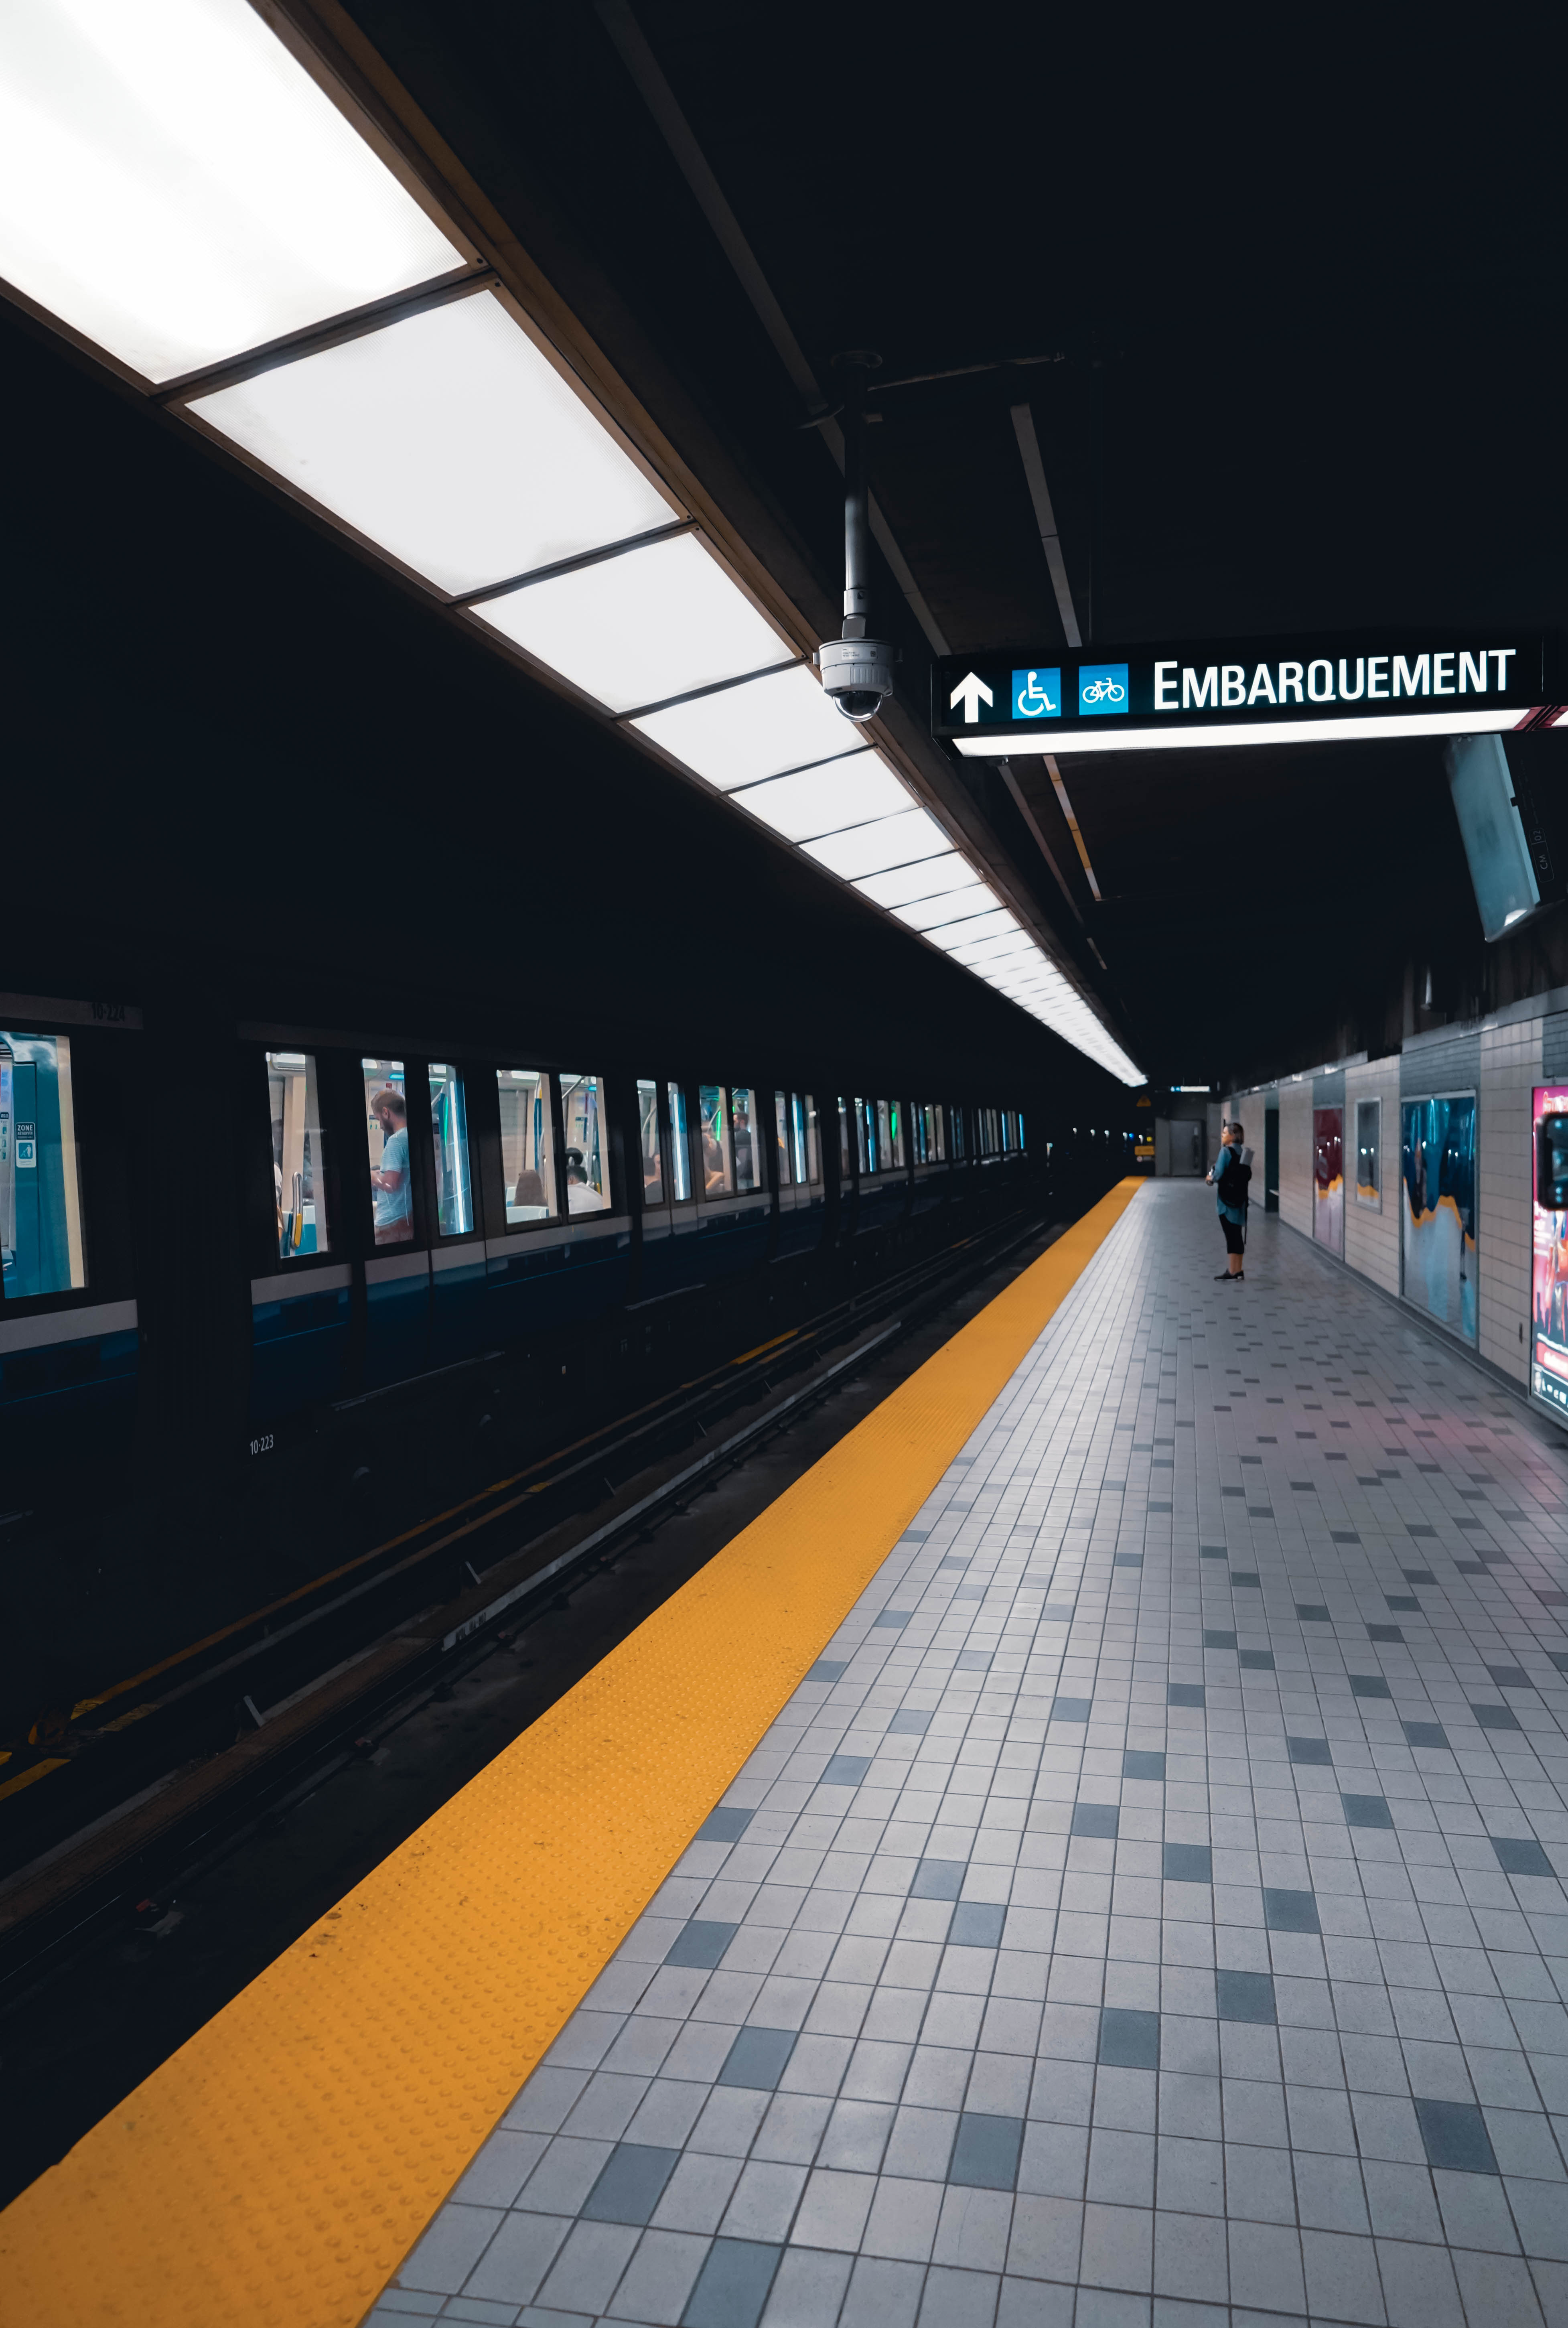
\includegraphics[width=\paperwidth,height=\paperheight]{src/Figures/Arriere_plan/Arriere_plan_Chap_3.jpg}
    }

% Rectangle
\AddToShipoutPictureBG*{
  \begin{tikzpicture}[remember picture,overlay]
    \node[fill=white, opacity=0.75, text width=\paperwidth, minimum height=7cm, anchor=north] 
    at ([yshift=-2cm]current page.north) {};
  \end{tikzpicture}
}

% Source
\AddToShipoutPictureFG*{
  \AtPageLowerRight{
    \raisebox{1cm}{
      \hspace{16cm}
      
\begin{tikzpicture}
        \node[fill=white, rounded corners=5pt, inner sep=5pt, align=center] {
          \tiny{Photographie~: \textcolor{blue}{Dylan Moinse (2022)}}
        };
      \end{tikzpicture}
    }
  }
}

    % ___________________________________________
    % Mini-sommaire
    \cleardoublepage
    \setcounter{tocdepth}{2}
    % Redéfinir le titre de la table des matières locale
    \renewcommand{\localcontentsname}{Table des matières du chapitre~3}
\localtableofcontents

% Réinitialiser numérotation section
\setcounter{section}{0}

    % ___________________________________________
    % Graphical abstract
    \newpage
\section*{Points clés du chapitre~3
    \label{chap3:graphical-abstract}
    }
    \markright{Préambule du chapitre}{}

\begin{figure}[h!]\vspace*{4pt}
        \caption*{}
        \label{graphical-abstract-chap3}
        \centerline{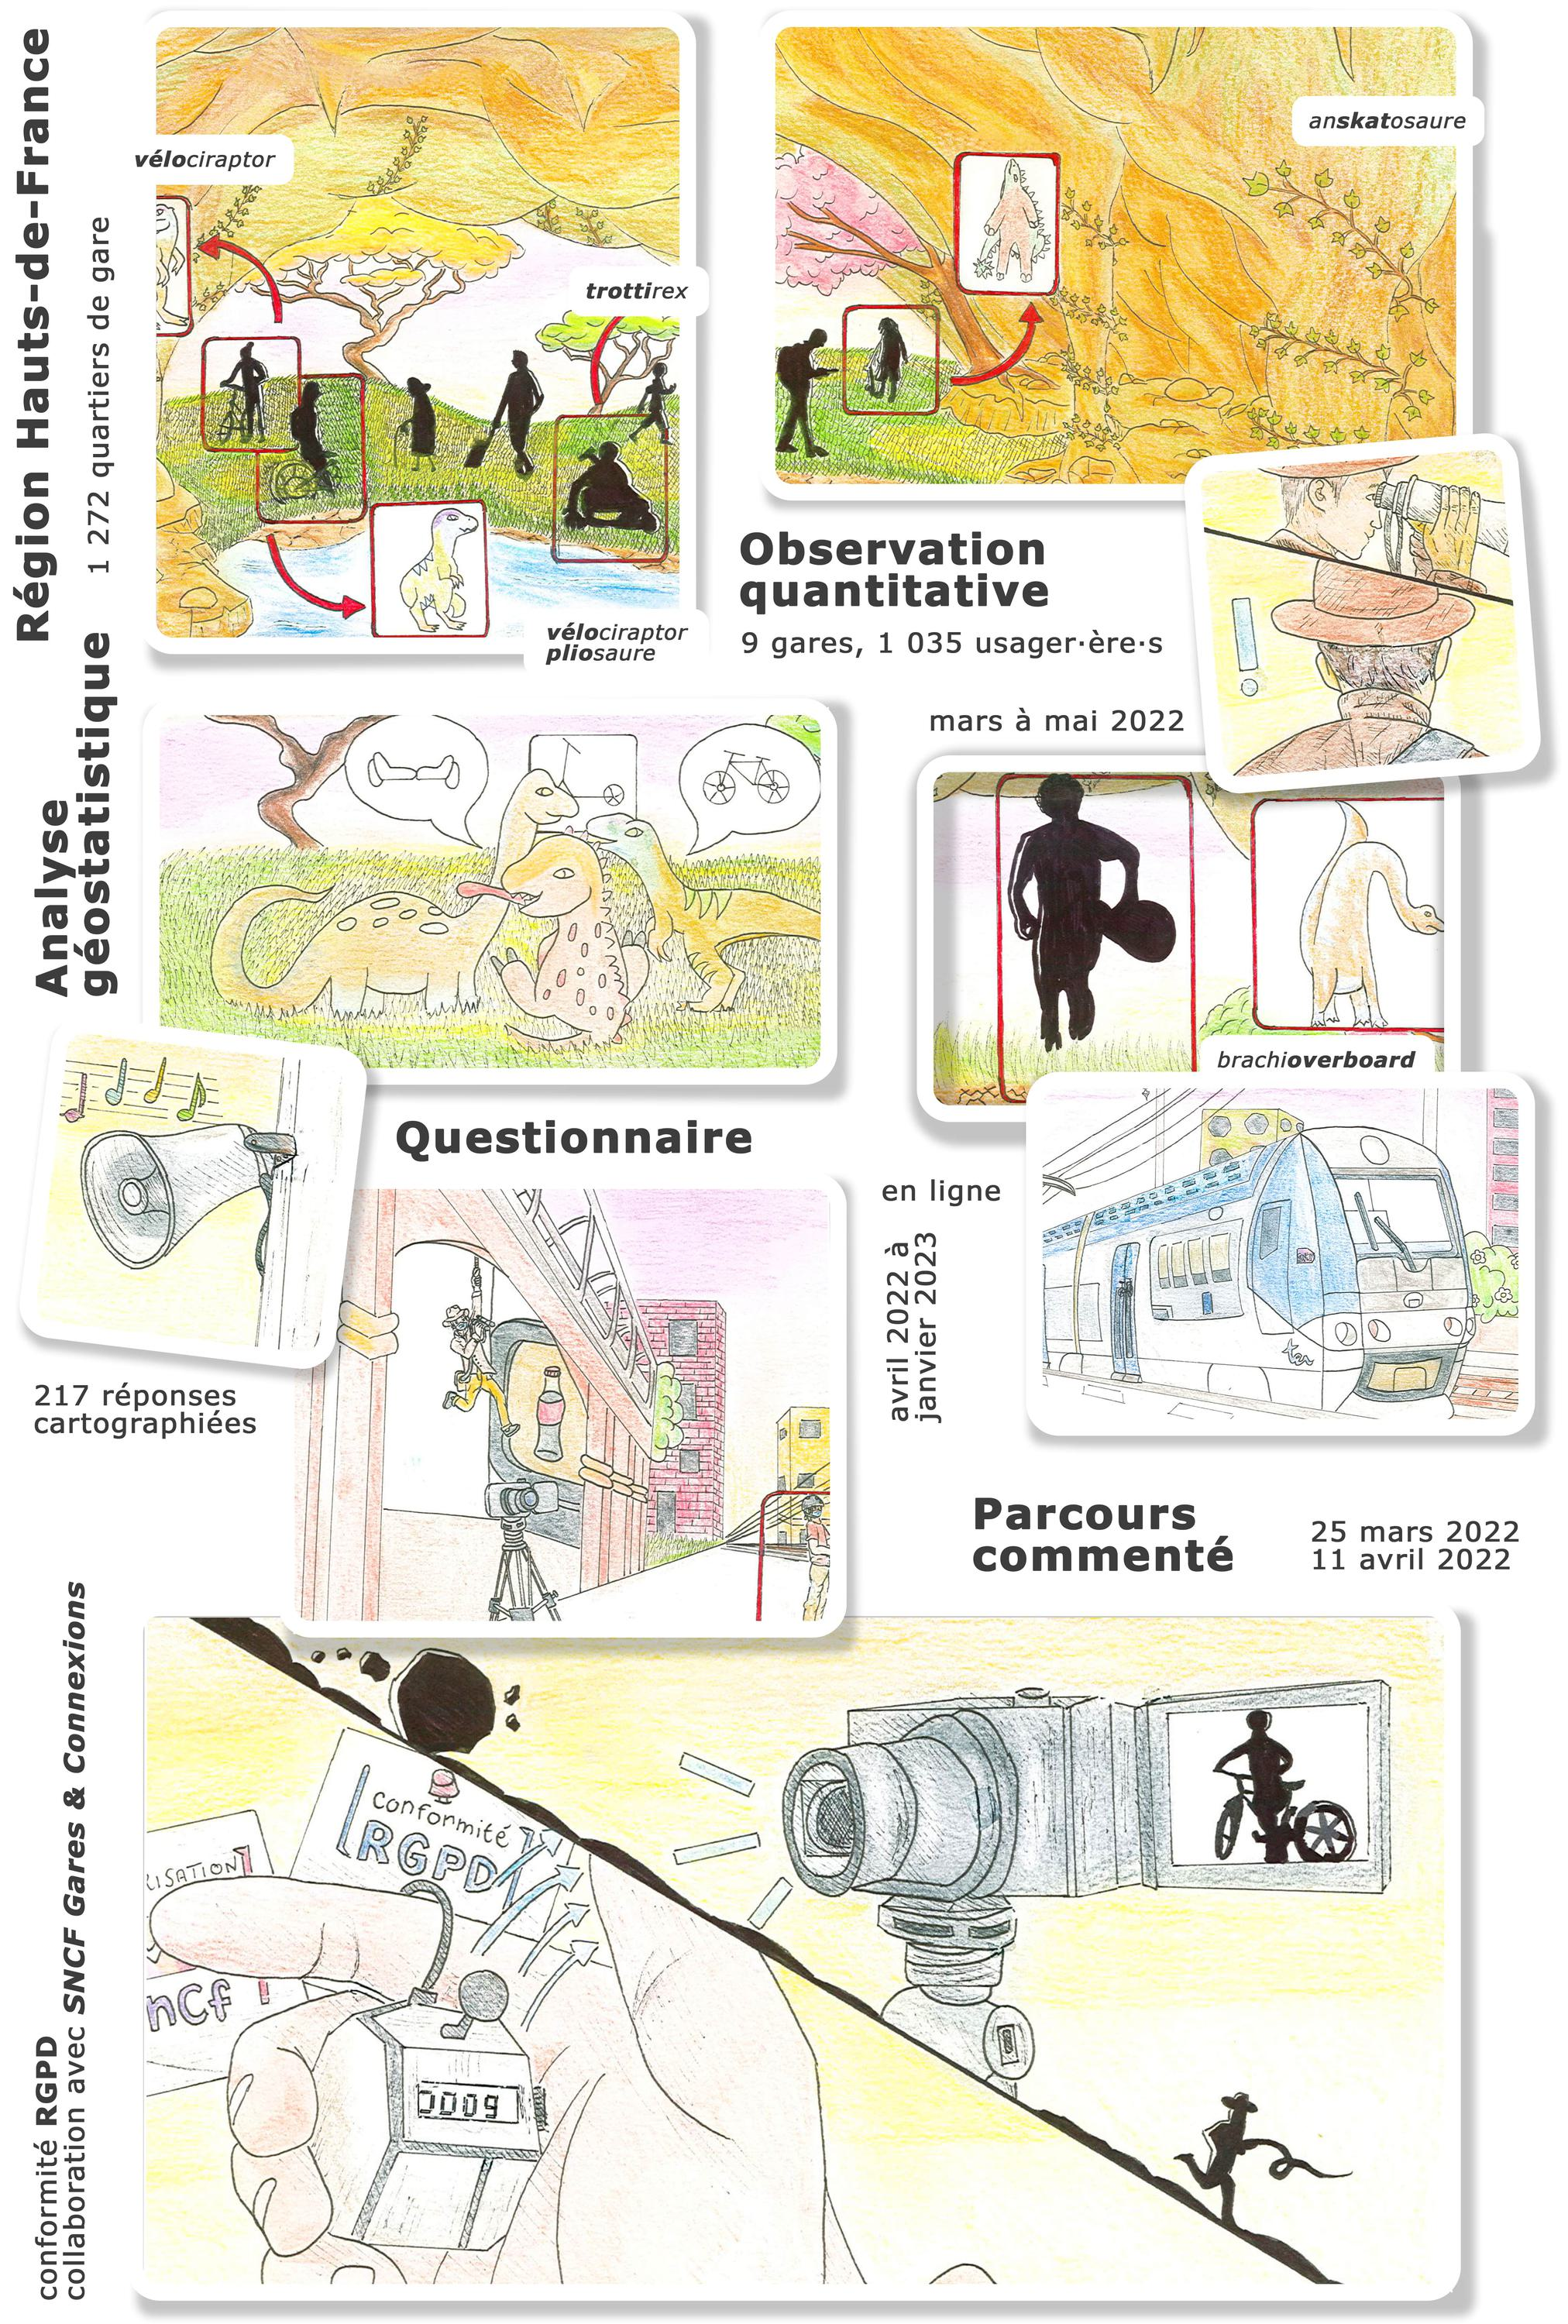
\includegraphics[width=1\columnwidth]{src/Figures/Graphical-abstract/FR_Graphical_abstract_chap3.jpg}}
        \vspace{5pt}
        \begin{flushright}\scriptsize{
        Source~: \textcolor{blue}{Morgan Moinse (2022)}
        }\end{flushright}
    \end{figure}

    % ___________________________________________
    % Préambule
    \newpage
    \begin{tcolorbox}[colback=white!5!white,
                      colframe=blue!75!blue,
                      title=
                      \bigskip
                      \center{\textbf{Préambule du chapitre~3}}
                      \\
                      \raggedright{\small{Chapitre composé de \pagedifference{chap3:titre}{part1:conclusion} pages, dont \pagedifference{chap3:bibliographie}{part1:conclusion} pages de bibliographie}}
                      \bigskip]
\Large{\textcolor{blue}{\textbf{Résumé~:}}}
    \\
    \small{
Ce chapitre présente la méthodologie développée pour enquêter sur les pratiques intermodales qui se déploient dans les quartiers de gare de la région des Hauts-de-France. En partant d'une contextualisation de notre étude de cas croisée à la description de nos recherches mixtes, nous avons cherché à concevoir une méthodologie basée sur une approche multidimensionnelle et multiscalaire. Structuré en cinq sections, le présent chapitre aborde successivement la définition du périmètre géographique, la projection spatiale des quartiers de gare ainsi que la mise en application d'une enquête croisant l'observation quantitative, l’administration d'un questionnaire et le parcours commenté.%%Rédigé%%
    \\
La première section établit les limites géographiques de l’étude et justifie le choix de la région Hauts-de-France comme cadre d’analyse (voir la \hyperref[chap3:region-hauts-de-france]{section~1}, page~\pageref{chap3:region-hauts-de-france}). Ce choix s’appuie sur son maillage ferroviaire dense et sa structure \textsl{a priori} polycentrique, bien qu’elle soit confrontée à des défis majeurs en matière de mobilité. Une attention particulière est portée à la posture réflexive du·de la chercheur·se et aux questions éthiques.%%Rédigé%%
    \\
Les quartiers de gare sont définis comme des unités spatiales théoriquement accessibles à pied ou à l'aide de la mobilité individuelle légère (voir la \hyperref[chap3:quartiers-gare]{section~2}, page~\pageref{chap3:quartiers-gare}). Une démarche spécifique, intégrant des critères spatiaux comme les distances acceptables et les caractéristiques de l’environnement urbain, est employée pour délimiter et cartographier ces zones d’influence. Cette approche permet d’examiner la configuration spatiale et fonctionnelle de ces espaces stratégiques grâce à des outils géostatistiques.%%Rédigé%%
    \\
Dans la troisième section, l’accent est mis sur l’observation quantitative des voyageur·se·s en gare, et plus particulièrement sur les usager·ère·s de la mobilité individuelle légère, souvent sous-représenté·e·s dans les enquêtes publiques (voir la \hyperref[chap3:observation-quantitative]{section~3}, page~\pageref{chap3:observation-quantitative}). Le protocole méthodologique, combinant comptage et observation ethnographique, est détaillé à travers des grilles d’observation appliquées dans neuf gares sélectionnées.%%Rédigé%%
    \\
La quatrième section traite de la conception et de l’administration d’un questionnaire destiné aux voyageur·se·s intermodaux·les (voir la \hyperref[chap3:questionnaire]{section~4}, page~\pageref{chap3:questionnaire}). Elle met en avant l’intérêt de cet outil pour collecter des données sur les pratiques de déplacement, les perceptions et les besoins exprimés. La structure du questionnaire, les étapes d’échantillonnage et la validation des réponses y sont détaillées, facilitant la mise en relation des déplacements déclarés avec les analyses géostatistiques et comportementales.%%Rédigé%%
    \\
Pour conclure, la cinquième section introduit l’approche des parcours commentés, une méthode qualitative menée \textsl{in situ}, permettant d’explorer les expériences des usager·ère·s en mouvement (voir la \hyperref[chap3:parcours-commente]{section~5}, page~\pageref{chap3:parcours-commente}). Elle vise à approfondir la compréhension des mécanismes de choix modal et des usages des infrastructures, sous l'angle de comptes rendus micro-géographiques.%%Rédigé%%
    }
    \tcblower
\Large{\textcolor{blue}{\textbf{Mots-clés~:}}}
    \\
    \small{
Analyse géostatistique~;
Hauts-de-France~;
Méthodes mixtes~;
Observation quantitative~;
Terrain de recherche~;
Parcours commentés~;
Questionnaire~;
Quartiers de gare
    }
    \end{tcolorbox}

    % ___________________________________________
    % 3.*.
    \newpage
    \needspace{1\baselineskip} % Réserve de l'espace
    \addcontentsline{toc}{section}{Introduction du chapitre~3}
    \sectionheader{Introduction du chapitre}
\section*{Introduction du chapitre~3
    \label{chap3:introduction}
    }
    \markright{Introduction du chapitre~3}{}

    % Citation
\begin{displayquote}
\Guillemets{[\dots] \textsl{par des processus créatifs (méthodes ad hoc) ou des synergies (entre méthodes déjà existantes), on parvient à affiner la qualité de l’observation, puis de l’analyse, selon le cas, d’une catégorie de comportements de déplacement quotidien ou de l’éventail des usages d’un réseau de transport. Les contributions témoignent de l’intérêt des chercheurs pour les questions de mobilité et de la grande créativité dont ils font preuve pour la saisir.} [\dots] \textsl{Pour le comprendre, l’analogie avec le microscope paraît assez parlante. Selon la focale qu’il choisit, l’image qu’un laborantin voit se former dans le microscope est à chaque fois différente. Il observe pourtant toujours la même réalité, mais à des échelles différentes ou, plus exactement, d’un point de vue différent. Ni l’une ni l’autre des images obtenues n’est plus vraie qu’une autre, mais elles rendent compte d’un regard différent sur la réalité.} [\dots] \textsl{Si la complémentarité des travaux de recherche quantitatifs et qualitatifs est louée de manière récurrente tel un idéal incantatoire, jusqu’à ce jour, peu de chercheurs la pratiquaient dans les faits.} [\dots] \textsl{Les innovations et hybridations méthodologiques renvoient de manière assez directe à la question des pratiques professionnelles des chercheurs. Nombreux sont, du reste, les articles à y faire référence explicitement. Ces innovations et hybridations sont le plus souvent réalisées en équipe, dans lesquelles chacune et chacun apporte ses pratiques, ses savoir-faire et ses compétences méthodologiques ou disciplinaires. Ce travail collectif, qui se reflète dans les contributions rassemblées ici, écrites pour la plupart par plusieurs auteurs, nécessite du temps et de la coordination pour partager les savoir-faire et les mettre en œuvre autour d’un dispositif opérationnalisable. Il nécessite également de l’audace et de la créativité pour pousser la porte de l’expérimentation et suffisamment de confiance, mais aussi d’humilité pour (re)connaître les valeurs et les limites de chaque méthode. Enfin, il suppose une capacité d’adaptation, de remise en question sous l’effet de stimulations multiples venues d’autres approches scientifiques, d’autres points de vue professionnels ou encore d’autres innovations venues des usages. Les innovations et hybridations méthodologiques apparaissent alors comme le reflet des capacités créatives des hommes, de leurs sociétés et de leurs territoires. C’est certainement dans ce travail créatif et fortement collaboratif que se nichent les innovations scientifiques de demain.}}

\textcolor{blue}{Joël} \textcolor{blue}{\textcite[12-14, 160]{meissonnier_connaissance_2020}}\index{Meissonnier, Joël|pagebf}\index{Vincent, Stéphanie|pagebf}\index{Rabaud, Mathieu|pagebf}\index{Kaufmann, Vincent|pagebf}. \textsl{Connaissance des mobilités~: hybridation des méthodes, diversification des sources}, Éditions du Cerema, Lyon, 176~p. ISBN~: \href{https://search.worldcat.org/fr/title/1236011015}{978-2-37180-423-4}
    \end{displayquote}

    % Introduction
\lettrine[lines=3, findent=8pt, nindent=0pt]{\lettrinefont L}{a} structuration de notre enquête repose sur l’observation des usages et l’explication des pratiques intermodales, avec une approche territoriale centrée sur la gare et son environnement, entendue comme l'interaction des dimensions environnementales, sociales et bâties dans un même système urbain, en référence à la notion d'\Guillemets{interconnexion des gares} \textcolor{blue}{\autocite[7]{moretti_interconnexion_1999}}\index{Moretti, Anna|pagebf}\index{Vacheret, Guy|pagebf}. Pour ce faire, notre méthodologie visant à étudier les gares, leur environnement et les usages qui s'y déploient privilégie une approche multidimensionnelle et multiscalaire. Cette démarche relationnelle articule trois niveaux d’observation~: (i) une logique relationnelle, axée sur la fonction de connexion des nœuds du réseau, (ii) une logique territoriale, portant sur les activités humaines polarisées et (iii) une logique d'usage, liant l'espace aux comportements des populations qui fréquent ces nœuds \textcolor{blue}{\autocites[9]{moretti_interconnexion_1999}[210-212]{menerault_gares_2001}}\index{Menerault, Philippe|pagebf}\index{Barré, Alain|pagebf}\index{Moretti, Anna|pagebf}\index{Vacheret, Guy|pagebf}. Notre ambition est ainsi de capturer le \Guillemets{système d’accessibilité territoriale} dans sa complexité, en intégrant l’\gls{accessibilité} \textsl{du} territoire et l’accessibilité \textsl{au} territoire, définies respectivement comme le potentiel spatial et social, et les interactions entre ces deux dimensions, structurées par la configuration de l'espace géographique et les caractéristiques des groupes sociaux \textcolor{blue}{\autocite[6]{richer_mesurer_2012}}\index{Richer, Cyprien|pagebf}\index{Palmier, Patrick|pagebf}. Nous avons alors mis à profit les atouts des approches quantitatives et qualitatives pour concevoir un cadre méthodologique intégré \textcolor{blue}{\autocite[]{bergman_advances_2008}}\index{Richer, Cyprien|pagebf}.%%Rédigé%%

    % Méthodes mixtes
Plutôt que de les opposer, les méthodes d’analyse des déplacements, qu’elles soient quantitatives ou qualitatives, gagneraient à être envisagées dans une logique de complémentarité \textcolor{blue}{\autocite[6]{klein_mobilites_2007}}\index{Klein, Olivier|pagebf}\index{Ortar, Nathalie|pagebf}\index{Pochet, Pascal|pagebf}. Un tel mode opératoire implique un partage disciplinaire davantage centré sur les objets d’étude. À cet égard, \textcolor{blue}{\textcite[4]{higgins_forty_2016}}\index{Higgins, Christopher~D.|pagebf}\index{Kanaroglou, Pavlos~S.|pagebf} soulignent tout l’intérêt d’un croisement entre les approches \Guillemets{normatives}, consistant à qualifier les types de \acrshort{TOD}, et les approches \Guillemets{positives} systématiques. C’est dans ce contexte que se justifie l’association de techniques méthodologiques variées que nous avons mise en œuvre, incluant l’exploitation de bases de données existantes conjuguée à des séances d’observation, à des enquêtes par questionnaire et à des entretiens \textsl{sur le terrain} \textcolor{blue}{\autocite[128]{dureau_lobservation_2014}}\index{Dureau, Françoise|pagebf}\index{Giroud, Matthieu|pagebf}\index{Lévy, Jean-Pierre|pagebf}. L’objectif de ces méthodes mixtes, d’un point de vue conceptuel, est de proposer une base exploratoire à partir de \textsl{l'action saisie} par l'intermédiaire de l'observation. Cette étape permet de concevoir et d'ajuster un questionnaire recueillant ce qui est \textsl{signifié}. Des réponses rapportées qui sont à leur tour interrogées au travers d'entretiens saisissant l'expérience telle qu'elle est \textsl{vécue et perçue} \textcolor{blue}{\autocite[215]{paugam_enquete_2012}}\index{Paugam, Serge|pagebf}.%%Rédigé%%

    % Description méthodes
Le croisement d’une enquête \Guillemets{sur-mesure}, intégrant une observation quantitative, un questionnaire et des parcours commentés destinés aux cyclo-voyageur·se·s, vise à fournir une perspective globale sur un sujet encore peu documenté par des données empiriques (pour rappel, voir le \hyperref[fig-introduction:methodes-hypotheses]{schéma~\ref{fig-introduction:methodes-hypotheses}}, au sein de l'\hyperref[introduction-generale:methodologie]{introduction générale}, page~\pageref{fig-introduction:methodes-hypotheses}). \textcolor{blue}{Joël} \textcolor{blue}{\textcite[24]{meissonnier_pour_2012}}\index{Meissonnier, Joël|pagebf}, autant que \textcolor{blue}{Karel} \textcolor{blue}{\textcite[291]{martens_bicycle_2004}}\index{Martens, Karel|pagebf} pour l'usage combiné du \gls{vélo} et du transport public, insistent sur l’importance de reconnaître les limites des enquêtes quantitatives classiques, à l'image de l’\acrfull{EMD}, lorsqu’il s’agit de rendre compte des dynamiques de mobilité quotidienne, et plus encore des chaînes de déplacement \textcolor{blue}{\autocite[10]{kieffer_chainage_2011}}\index{Kieffer, Lionel|pagebf}\index{Oliveau, Sébastien|pagebf}\index{Audard, Frédéric|pagebf}. Cela demande de repenser l'approche en enrichissant les bases de données actuelles grâce à des enquêtes de terrain adaptées aux exigences de notre problématique de recherche. Cette démarche s’appuie sur des travaux préexistants qui ont ouvert la voie et inspiré notre méthodologie. Par exemple, \textcolor{blue}{François de} \textcolor{blue}{\textcite[42]{singly_questionnaire_2016}}\index{Singly, François de|pagebf} souligne l’intérêt, en sciences sociales, de combiner le questionnaire, qui rend visibles les déterminants sociaux des trajectoires, avec les entretiens, qui éclairent sur le processus de construction individuelle de ces trajectoires. Ainsi, plusieurs études ont démontré l’intérêt de mobiliser une méthodologie mixte articulant observation directe, questionnaire et entretiens \Guillemets{mobiles} \textcolor{blue}{\autocites[258]{greene_toward_1989}[120]{bergeron_uncovering_2014}[3]{despres_replacer_2019}}\index{Greene, Jennifer~C.|pagebf}\index{Caracelli, Valerie~J.|pagebf}\index{Graham, Wendy~F.|pagebf}\index{Bergeron, Julie|pagebf}\index{Paquette, Sylvain|pagebf}\index{Poullaouec-Gonidec, Philippe|pagebf}\index{Desprès, Michel|pagebf}\index{Lord, Sébastien|pagebf}\index{Negron-Poblete, Paula|pagebf}.%%Rédigé%%

    % Annonce du plan 1
La première partie du présent chapitre porte sur la délimitation du terrain géographique, envisagée sous un prisme macroscopique (\hyperref[chap3:region-hauts-de-france]{section~1}, page~\pageref{chap3:region-hauts-de-france}). Cette démarche vise à justifier la pertinence d’une perspective régionale en présentant les enjeux de mobilité ainsi que les documents stratégiques établis par l’autorité administrative compétente (\hyperref[chap3:regard-privilegie-region-hdf]{sous-section~1.1}, page~\pageref{chap3:regard-privilegie-region-hdf}). Dans un second temps, un exercice d’auto-analyse sociologique sera mené afin d’objectiver notre positionnement vis-à-vis du terrain, compris à la fois comme sujet de recherche et contexte géographique (\hyperref[chap3:auto-analyse-sociologique]{sous-section~1.2}, page~\pageref{chap3:auto-analyse-sociologique}). La description du périmètre géographique dans lequel s’inscrit notre matériau empirique se conclura par notre mise en relation avec le gestionnaire principal de mobilité et par la mise en conformité de nos méthodes d’enquête avec les principes de l’éthique de la recherche (\hyperref[chap3:preparation-terrain-geographique]{sous-section~1.3}, page~\pageref{chap3:preparation-terrain-geographique}).%%Rédigé%%

    % Annonce du plan 2
Une fois le cadre géographique introduit, nous nous attacherons à détailler le processus de spatialisation des quartiers de gare, entendus comme unités spatiales accessibles à pied et en mobilité individuelle légère, dans une perspective microscopique (\hyperref[chap3:quartiers-gare]{section~2}, page~\pageref{chap3:quartiers-gare}). Nous définirons les règles méthodologiques permettant de cartographier ces aires d’influence, en nous basant sur les distances jugées acceptables et sur la typologie des gares dressée, telles qu’elles auront été déterminées grâce à notre enquête de terrain (\hyperref[chap3:quartiers-gare-distances]{sous-section~2.1}, page~\pageref{chap3:quartiers-gare-distances}). Une fois les tailles des quartiers de gare définies, notre attention se portera sur leurs formes et leurs contours, influencées par les caractéristiques de l’environnement bâti. Cette étape inclura une réflexion sur les méthodes employées pour générer et représenter ces formes (\hyperref[chap3:quartiers-gare-formes]{sous-section~2.2}, page~\pageref{chap3:quartiers-gare-formes}). Pour clore cette section, nous présenterons les principes d’extraction et de traitement des données géostatistiques que nous nous serons fixés. Nous exposerons les critères retenus pour exploiter les bases de données, en nous efforçant d'obtenir un degré de résolution élevé de l'information géographique (\hyperref[chap3:quartiers-gare-analyse-geostatistique]{sous-section~2.3}, page~\pageref{chap3:quartiers-gare-analyse-geostatistique}).%%Rédigé%%

    % Annonce du plan 3
La troisième section de notre chapitre méthodologique sera consacrée à la description de l’approche par observation quantitative des cyclo-voyageur·se·s, dans l’objectif de dresser un panorama général et d’évaluer les tendances actuelles, alors encore peu documentées (\hyperref[chap3:observation-quantitative]{section~3}, page~\pageref{chap3:observation-quantitative}). Premièrement, nous définirons ce qu’est une observation quantitative, en explicitant son adéquation avec certains de nos objectifs de recherche (\hyperref[chap3:observation-quantitative-outil-adapte]{sous-section~3.1}, page~\pageref{chap3:observation-quantitative-outil-adapte}). Ensuite, nous détaillerons le protocole méthodologique de notre démarche mêlant comptage et observation ethnographique. Nous présenterons à cette occasion la grille d’observation utilisée et les modalités de sa mise en application (\hyperref[chap3:methodologie-observation-quantitative]{sous-section~3.2}, page~\pageref{chap3:methodologie-observation-quantitative}). La section prend fin avec la contextualisation des neuf gares examinées dans le cadre de cette enquête, au sein de laquelle nous justifierons leur sélection (\hyperref[chap3:observation-quantitative-gares-examinees]{sous-section~3.3}, page~\pageref{chap3:observation-quantitative-gares-examinees}).%%Rédigé%%

    % Annonce du plan 4
À la suite de l’observation quantitative, nous introduirons le questionnaire s’adressant aux usager·ère·s (\hyperref[chap3:questionnaire]{section~4}, page~\pageref{chap3:questionnaire}). Nous appuierons la plus-value de cet outil méthodologique (\hyperref[chap3:apports-questionnaire-usagers]{sous-section~4.1}, page~\pageref{chap3:apports-questionnaire-usagers}). Nous détaillerons ensuite le processus d’administration du questionnaire, en présentant sa structure générale, le processus d’échantillonnage ainsi que la validation des réponses obtenues, dont les déplacements déclarés ont pu être projetés (\hyperref[chap3:administration-questionnaire-usagers]{sous-section~4.2}, page~\pageref{chap3:administration-questionnaire-usagers}).%%Rédigé%%

    % Annonce du plan 5
La troisième approche de notre enquête de terrain, qui sera exposée au fil de cette thèse, repose sur une première exploration des parcours commentés (\hyperref[chap3:parcours-commente]{section~5}, page~\pageref{chap3:parcours-commente}). Tout d'abord, nous resituerons cette méthode d’entretien \textsl{in situ}, en mettant l’accent sur ses différentes déclinaisons (\hyperref[chap3:parcours-commente-definition]{sous-section~5.1}, page~\pageref{chap3:parcours-commente-definition}). Ensuite, nous montrerons comment cette méthode a été adaptée à notre terrain d’enquête, au prisme des comptes rendus \Guillemets{micro-géographiques} générés (\hyperref[chap3:parcours-commente-administration-participants]{sous-section~5.2}, page~\pageref{chap3:parcours-commente-administration-participants}).%%Rédigé%%

    % Annonce du plan 6
Pour conclure, nous replacerons les diverses approches dans une vision d’ensemble, pour illustrer leur articulation et leur connexion avec nos hypothèses de recherche (\hyperref[chap3:conclusion]{conclusion du chapitre~3}, page~\pageref{chap3:conclusion}).%%Rédigé%%

     % ___________________________________________
    % 3.1.
    \newpage
    \needspace{1\baselineskip} % Réserve de l'espace
    \sectionheader{Mise en contexte de la région Hauts-de-France}
\section{Délimitation du terrain géographique défini par le périmètre de la région Hauts-de-France
    \label{chap3:region-hauts-de-france}
    }

    % Introduction
Entrer par le terrain nécessite avant tout de motiver le choix de ce périmètre et de le replacer dans son contexte pour en comprendre les caractéristiques locales et les enjeux territoriaux. Cette démarche implique également une introspection sur notre propre rapport, à la fois personnel et éthique, aux lieux explorés et aux personnes interrogées. Cette première section vise ainsi à délimiter le cadre géographique de notre recherche empirique, tout en explicitant les fondements de notre posture méthodologique. Une étude sous l'angle du \acrshort{TOD} révèle tout son intérêt lorsqu’elle s’inscrit dans une approche régionale, dans le souci d'établir une vision globale du développement régional \textcolor{blue}{\autocite[24]{lo_feudo_scenario_2014}}\index{Lo Feudo, Fausto|pagebf}\index{Menerault, Philippe|pagebf}\index{L'Hostis, Alain|pagebf}\index{Festa, Demetrio Carmine|pagebf}. Le transport public, et plus particulièrement le fer, constitue un levier structurant pour l'aménagement régional, perçu dans les Hauts-de-France comme un \Guillemets{capital spatial porteur de multiples opportunités} \textcolor{blue}{\autocite[147, 163]{baron_reseaux_2017}}\index{Baron, Nacima|pagebf}\index{Messulam, Pierre|pagebf}. Comme en témoignent les orientations définies par la \textcolor{blue}{\textcite[17]{region_hauts-de-france_planification_2024}}\index{Région Hauts-de-France@\textsl{Région Hauts-de-France}|pagebf}, dont l'ambition est de \Guillemets{\textsl{faire du réseau régional des transports l'épine dorsale de la mobilité en Hauts-de-France} [\dots] \textsl{s'appuyant prioritairement sur le réseau régional structurant (lignes ferroviaires et routières)} [\dots] [avec un système de] \textsl{rabattement vers ceux-ci par des modes pertinents}}.%%Rédigé%%

    % Annonce du plan
Premièrement, nous commencerons par expliquer et décrire la situation et les enjeux de la région Hauts-de-France, qui constitue le cadre géographique de cette recherche (voir la \hyperref[chap3:regard-privilegie-region-hdf]{section sur le regard privilégié sur la région Hauts-de-France}, page~\pageref{chap3:regard-privilegie-region-hdf}). Par le biais de cette exploration détaillée du territoire régional, nous aurons la possibilité de construire une posture d'objectivation scientifique appuyée sur une méthode d'\Guillemets{auto-analyse sociologique} (voir la \hyperref[chap3:auto-analyse-sociologique]{section sur la réflexivité sociologique}, page~\pageref{chap3:auto-analyse-sociologique}). Nous traiterons également des aspects éthiques de notre recherche empirique, en décrivant les actions entreprises pour assurer leur respect de ces principes dans nos interactions avec les acteur·rice·s locaux·les et avec les terrains investis (voir la \hyperref[chap3:preparation-terrain-geographique]{section sur la conformité à l’éthique de la recherche}, page~\pageref{chap3:preparation-terrain-geographique}).%%Rédigé%%

    % 3.1.1.
    \needspace{1\baselineskip} % Réserve de l'espace
\subsection{Recherche-action et territoires de l'action publique~: regard privilégié sur la région Hauts-de-France
    \label{chap3:regard-privilegie-region-hdf}
    }

    % Introduction
Dans le contexte français, et pour une majorité de chercheur·se·s en géographie, la région est souvent considérée comme l'unité territoriale fondamentale dans le fonctionnement du système économique globalisé \textcolor{blue}{\autocite[]{calthorpe_regional_2001}}\index{Calthorpe, Peter|pagebf}\index{Fulton, William|pagebf}. Cependant, cette conception soulève une question importante~: se réfère-t-on à une \textsl{région urbaine} ou \textsl{fonctionnelle}, au sens des flux quotidiens, ou à une \textsl{région politique}, inscrite dans des découpages administratifs~? Inscrit dans le programme de transition écologique et connectée \textsl{rev3} (\textsl{Troisième Révolution Industrielle})\footnote{
    Le XXI\textsuperscript{e} siècle est marqué par la \textsl{Troisième Révolution Industrielle}, en référence à l'ouvrage de l'économiste \textcolor{blue}{Jeremy} \textcolor{blue}{\textcite[338]{rifkin_troisieme_2012}}\index{Rifkin, Jeremy|pagebf}, dont l'un des cinq piliers repose sur l'émergence d'une économie numérique et électrique qui s'exprime en partie par le partage de transports connectés. Pour l'auteur, la \textsl{Troisième Révolution Industrielle} bouscule les manières de concevoir et de pratiquer la mobilité urbaine. C'est dans ce cadre que l'auteur a été sollicité pour imaginer une feuille de route pour la Région Hauts-de-France. L'acronnyme \textsl{rev3}, piloté par la Région et la \acrfull{CCI} Hauts-de-France, est l'appellation donnée à cette politique menée dans les Hauts-de-France qui propose des modèles de développement des territoires et de la mobilité à l'horizon 2050.
}, le présent projet doctoral pourrait légitimement être centré sur la région institutionnelle. Toutefois, d'autres arguments viennent étayer le choix assumé de nous concentrer sur la région administrative, comme développé dans la thèse de doctorat de \textcolor{blue}{Julia} \textcolor{blue}{\textcite[166]{frotey_acteurs_2021}}\index{Frotey, Julia|pagebf}\index{Deboudt, Philippe|pagebf}\index{Castex, Élodie|pagebf}\index{Frère, Séverine|pagebf} sur le développement de l'électromobilité dans les Hauts-de-France. Historiquement, la géographie s'est efforcée de s'éloigner des découpages politiques pour mieux appréhender la complexité du fonctionnement des espaces, en tenant compte des flux et des échanges qui les traversent \textcolor{blue}{\autocite[]{pumain_regionalisation_2016}}\index{Pumain, Denise|pagebf}. Cette prise de distance, particulièrement marquée après-guerre~–~\textcolor{blue}{\textcite[16-18]{menerault_reseaux_1991}}\index{Menerault, Philippe|pagebf}\index{Dupuy, Gabriel|pagebf} parlant d'\Guillemets{éclipse} dans ses travaux doctoraux~–~s'est atténuée à partir des années 1970, lorsque la géographie politique a retrouvé un intérêt pour les territoires, envisagés comme des formes d'organisation de l'espace liées à l'action publique.%%Rédigé%%

    % Géographie régionale
Plus largement, cette réflexion autour de l’échelle régionale institutionnelle s’inscrit dans le cadre de la géographie régionale. Elle trouve écho dans le long processus de décentralisation amorcé en France, ainsi que dans le contexte récent de fusion des régions. Comme le rappelle \textcolor{blue}{Nicole} \textcolor{blue}{\textcite[107]{girard_region_2004}}\index{Girard, Nicole|pagebf}, la géographie est \Guillemets{[\dots] \textsl{sans doute une des disciplines universitaires les plus \Guillemets{régionalées}, au sens où, depuis longtemps, son implantation régionale est affirmée} [\dots]}. En France, la notion de \Guillemets{région} s’associe désormais principalement au cadre politico-administratif, s’éloignant ainsi de la \Guillemets{région naturelle}, dans laquelle ont lieu les relations homme-milieu, chère à la géographie vidalienne et à l’École française de géographie \textcolor{blue}{\autocite[391]{mercier_entre_2001}}\index{Mercier, Guy|pagebf}. À cet égard, la région, en tant qu’entité politico-administrative et spatiale, s’impose progressivement tant aux citoyen·ne·s qu’aux chercheur·se·s comme une réalité incontournable \textcolor{blue}{\autocite[111]{girard_region_2004}}\index{Girard, Nicole|pagebf}. Pour ces raisons, cette thèse adopte l’échelle administrative de la région comme référentiel géographique, nous permettant de nous appuyer sur une échelle institutionnelle adaptée à notre sujet de recherche, positionnée au cœur de l’emboîtement des échelons, et d'accéder à des bases de données ouvertes, qu'il est parfois rare de trouver autrement.%%Rédigé%%

    % 3.1.1.1.
    \needspace{1\baselineskip} % Réserve de l'espace
\subsubsection*{Intérêt d'une approche régionale du \textsl{Transit-Oriented Development}
    \label{chap3:approche-regionale}
    }

    % TOD et train
\textcolor{blue}{Peter} \textcolor{blue}{\textcite[62, 67, 104]{calthorpe_next_1993}}\index{Calthorpe, Peter|pagebf} distingue fondamentalement deux échelles géographiques d'application du \acrshort{TOD}~: une première sur un plan interurbain ou régional et une seconde centrée sur le \Guillemets{quartier} (\textsl{neighborhood}), conférant une dimension multiscalaire à ce concept d’aménagement. Cette approche reflète l’influence du mouvement de la \textsl{Smart Growth}, qui valorise une planification orientée vers un développement régional de l’urbanisation \textcolor{blue}{\autocite[70]{dushina_tod_2015}}\index{Dushina, Anna|pagebf}\index{Paulhiac, Florence|pagebf}\index{Scherrer, Franck|pagebf}. La question de l’échelle géographique d’application du \acrshort{TOD} est déterminante. Et pour cause, limiter l’analyse à un quartier de gare isolé exclut la logique multiscalaire de connectivité à des échelles plus larges \textcolor{blue}{\autocite[273]{menerault_gares_2001}}\index{Menerault, Philippe|pagebf}\index{Barré, Alain|pagebf}. Une approche régionale inscrit ainsi le \acrshort{TOD} dans une perspective de planification polycentrique\footnote{
    Un large débat scientifique remet en question les vertus souvent attribuées aux systèmes urbains polycentriques pour réduire les flux de mobilité carbonés, en particulier les déplacements quotidiens longs. \textcolor{blue}{\textcite[515]{richardson_discourses_2000}}\index{Richardson, Tim|pagebf}\index{Jensen, Ole~B.|pagebf} parlent d'un \Guillemets{récit spatial} (\textsl{spatial narrative}) pour décrire les orientations des politiques de planification européennes en faveur de configurations territoriales polycentriques. Ces politiques promeuvent le polycentrisme, qui repose sur une organisation urbaine avec plusieurs centres ou pôles d'activité. Ce modèle est censé limiter les déplacements longue distance, généralement réalisés en voiture, en rapprochant les habitant·e·s de leurs lieux de travail, des services essentiels et des opportunités économiques. En outre, il permet une meilleure répartition des flux de mobilité et une optimisation des réseaux de transport grâce à la combinaison de réseaux radiaux et de ceintures inter-pôles. Ce modèle contribue également à une meilleure équité territoriale, en réduisant les disparités d'accès depuis les territoires périphériques. Cependant, des recherches empiriques, telles que celles d’\textcolor{blue}{Anne} \textcolor{blue}{\textcite[1~545]{aguilera_growth_2005}}\index{Aguiléra, Anne|pagebf} pour Paris, Lyon et Marseille~; ou de \textcolor{blue}{Florent} \textcolor{blue}{\textcite{le_nechet_modelling_2019}}\index{Le Néchet, Florent|pagebf} pour l'Île-de-France et la Ruhr, démontrent que les systèmes polycentriques, en dispersant les flux de mobilité, compliquent la planification des réseaux de \gls{transport en commun}, souvent moins efficace que dans un modèle monocentrique où les flux convergent vers un centre unique. Par ailleurs, la gouvernance de ces systèmes s'avère complexe, en raison des enjeux inter-territoriaux qu'ils impliquent. Enfin, le polycentrisme peut engendrer un effet rebond, favorisant des pratiques de navettage inter-pôles et, paradoxalement, une augmentation globale des déplacements.
}, plus cohérente dans le déploiement de systèmes alternatifs de mobilité, tels que le système ferroviaire pertinent dans le contexte européen \textcolor{blue}{\autocite[212]{bertolini_sustainable_2005}}\index{Bertolini, Luca|pagebf}\index{Le Clercq,~F.|pagebf}\index{Kapoen,~L.|pagebf}. Dans la pratique, le \acrshort{TOD} est effectivement interprété différemment selon les contextes géographiques. Aux États-Unis, les projets qui se revendiquent du \acrshort{TOD} et déployés dans les métropoles se concentrent sur des infrastructures \Guillemets{légères} comme le tramway ou les systèmes de \acrfull{BHNS}, tandis qu’en Europe, notamment en France, le système ferroviaire est plus adapté à une échelle régionale \textcolor{blue}{\autocite[95]{bonin_evaluation_2015}}\index{Bonin, Olivier|pagebf}\index{Tomasoni, Lorenza|pagebf}. Par exemple, \textcolor{blue}{Alexis} \textcolor{blue}{\textcite[132]{conesa_accessibility_2018}}\index{Conesa, Alexis|pagebf} illustre, dans le cas de l’ancienne région Nord-Pas-de-Calais, comment certaines lacunes d’accessibilité locale peuvent être atténuées en renforçant la connectivité de la gare au réseau, grâce à la portée régionale du \acrshort{TOD}.%%Rédigé%%

    % TOD et région urbaine
Le choix d’un terrain régional permet de replacer les gares dans une dynamique de développement urbain plus vaste. L’hypothèse centrale contenue dans les recherches régionales sur le \acrshort{TOD} repose sur une démarche visant à articuler les échelles spatiales et temporelles au sein du couple gare et quartier de gare \textcolor{blue}{\autocite[14]{menerault_gares_2001}}\index{Menerault, Philippe|pagebf}\index{Barré, Alain|pagebf}. Il est postulé que le niveau de développement d’une station est intrinsèquement lié à sa position dans le réseau \textcolor{blue}{\autocite[344]{bertolini_nodes_1996}}\index{Bertolini, Luca|pagebf}. Dans cette perspective, \textcolor{blue}{Florent} \textcolor{blue}{\textcite[5]{le_nechet_modelling_2019}}\index{Le Néchet, Florent|pagebf}, explorant l’articulation entre réseau et formes urbaines dans le cadre des \Guillemets{régions métropolitaines} (\textsl{Mega-City Regions}), a démontré que la coordination et la gestion des projets urbains devient plus efficiente lorsque les acteurs actifs dans ces structures institutionnelles sont impliqués, à la différence d'une somme d'initiatives locales éclatées. Ce raisonnement est partagé par \textcolor{blue}{\textcite[55, 111]{singh_measuring_2015}}\index{Singh, Yamini Jain|pagebf}\index{Maarseveen, Martin van|pagebf}\index{Zuidgeest, Mark|pagebf}\index{Flacke, Johannes|pagebf}, dans sa thèse de doctorat sur la mesure du \acrshort{TOD} à l'Université de Twente, qui plaide en faveur d’une analyse duale des échelles spatiales, afin d’intégrer de manière optimale les services de transport et les dynamiques urbaines.%%Rédigé%%

    % Compétences régions
En France, la région constitue un échelon approprié pour déployer une stratégie d'aménagement orientée vers les transports en commun, en raison de ses compétences diversifiées, consolidées par un cadre juridique en matière de transport et de planification. Elle a d'abord pour vertu de faire exister un territoire de projet en fédérant, dans un cadre de référence commun, des initiatives auparavant menées de manière séparée. Les contrats d’axe, par exemple, permettent de dépasser la logique de guichet qui a longtemps caractérisé les relations entre les régions et les communes \textcolor{blue}{\autocite[118]{bentayou_contrat_2015}}\index{Bentayou, Gilles|pagebf}\index{Perrin, Emmanuel|pagebf}\index{Richer, Cyprien|pagebf}. C'est depuis l’entrée en vigueur du premier instrument législatif positionnant la région au centre des politiques de transport, la \acrfull{LOTI}\footnote{
    À partir d'une première expérimentation sur la régionalisation du chemin de fer menée dans l'ancienne région Nord-Pas-de-Calais en 1978 \textcolor{blue}{\autocites[I-3]{chauvineau_regionalisation_2001}[424]{passavant-guion_financer_2016}}\index{Chauvineau, Jacques|pagebf}\index{Passavant-Guion, Lisa|pagebf}\index{Négrier, Emmanuel|pagebf}, la \acrfull{LOTI} du 30 décembre 1982, amorce un processus de décentralisation en instaurant une nouvelle répartition des compétences entre l'État et les collectivités locales. Cette loi ouvre la voie de la régionalisation des \Guillemets{liaisons ferroviaires d'intérêt régional}, par le biais du conventionnement entre les régions et la SNCF \textcolor{blue}{\autocite[4]{deimon_projets_2024}}\index{Deimon, Tristan Buteau|pagebf}. Le commencement de ce long processus, initié dès 1974 par les schémas régionaux de transport, aboutit au lancement du \acrfull{TER} en 1987. Pour autant, la décentralisation des services ferroviaires reste facultative \textcolor{blue}{\autocite{commission_nationale_du_debat_public_chronologie_nodate}}. À la suite de la promulgation de la \acrfull{LOADT} du 4 février 1995, reprise et modifiée dans la \acrfull{LOADDT} du 25 juin 1999, sept régions, dont le Nord-Pas-de-Calais, se portent candidates à partir de 1997 pour expérimenter la gestion du transport ferroviaire régional \textcolor{blue}{\autocite[132]{burlando_regionalisation_2004}}\index{Burlando, Claudia|pagebf}\index{Guihéry, Laurent|pagebf}.
} qui a posé le principe du partage des responsabilités entre l'État et les collectivités locales. Mais il s'agit surtout de la \acrfull{SRU} du 13 décembre 2000\footnote{
    La généralisation de la régionalisation ferroviaire est prévue en 2002, en vue des dispositions appliquées par la \acrfull{SRU} et de la publication du décret relatif au \Guillemets{transfert des compétences en matière de transport collectif d'intérêt régional} du 27 novembre 2001 \textcolor{blue}{\autocite[132]{burlando_regionalisation_2004}}\index{Burlando, Claudia|pagebf}\index{Guihéry, Laurent|pagebf}. La loi prévoit alors le développement d'une coopération entre la région et les autorités urbaines afin d'organiser l'intermodalité~: la création de comités de partenaires du transport public vise ainsi à améliorer la continuité entre le système ferroviaire et les systèmes de transport urbain. C'est dans ce cadre que l'échelon régional tend à s'affirmer comme autorité organisatrice \Guillemets{cheffe de file} \textcolor{blue}{\autocite[I-18]{chauvineau_regionalisation_2001}}\index{Chauvineau, Jacques|pagebf}.
}, qui consacre la région en tant qu'\Guillemets{organisatrice des transports collectifs d'intérêt général}, à l'exclusion de l'Île-de-France et de la Corse \textcolor{blue}{\autocite{commission_nationale_du_debat_public_chronologie_nodate}}\index{Commission nationale du débat public@\textsl{Commission nationale du débat public}|pagebf}. L'acte~III de la décentralisation se matérialise par la \acrfull{MAPTAM} du 27 janvier 2014 portant la \acrfull{NOTRe} du 7 août 2015\footnote{
    Avec la \acrfull{MAPTAM}, l'échelon régional est chargé de coordonner son action avec celle des autres autorités organisatrices de la mobilité tout en définissant des règles générales relatives à l'intermodalité entre les services publics de transport, dans le cadre du \acrfull{SRI} \textcolor{blue}{\autocite{gart_aom_nodate}}. Par ailleurs, la loi redessine les contours de certaines régions françaises, dont celles du Nord-Pas-de-Calais et de la Picardie, en les fusionnant. Ces changements constituent une opportunité pour les régions nouvellement fusionnées de repenser leur offre et leur politique de transport sur leur périmètre élargi \textcolor{blue}{\autocite{cerema_mobilite_2017}}. En parallèle, la loi \acrfull{NOTRe} renforce ce volet de transfert de compétences en créant un outil de planification à l'échelle de la région, le \acrfull{SRADDET}.
} qui consacre la région comme \Guillemets{cheffe de file de l'intermodalité et de la complémentarité entre les modes de transports} \textcolor{blue}{\autocite{gart_aom_nodate}}\index{GART@\textsl{GART}|pagebf}. Récemment, son cadre d'intervention a été renforcé grâce à la \acrfull{LOM} du 24 décembre 2019\footnote{
    Quarante ans après le texte fondamental d'organisation des services publics de transport (loi \acrshort{LOTI}), la \acrfull{LOM} cherche à appliquer une répartition entre les 1~200 autorités locales, appelées \acrfull{AOM}, et les 12 \acrshort{AOM} régionales chargées notamment du \acrshort{TER} et des car interurbains \textcolor{blue}{\autocite[29]{richer_quoi_2024}}\index{Richer, Cyprien|pagebf}\index{Pitout, Nicolas|pagebf}\index{Fabry, Alexandre|pagebf}. Dans le mouvement de décentralisation, la région demeure un acteur relativement jeune dont le poids politique ne cesse d'augmenter à mesure que les réformes territoriales lui confèrent de nouvelles compétences~: aujourd'hui, la région devient \Guillemets{un peu l'acteur à tout faire en matière de mobilité} \textcolor{blue}{\autocite[34]{richer_quoi_2024}}\index{Richer, Cyprien|pagebf}\index{Pitout, Nicolas|pagebf}\index{Fabry, Alexandre|pagebf}. Il en va que la \acrshort{LOM} promeut un \Guillemets{droit à la mobilité}, en référence au précédent \Guillemets{droit au transport} institué par la \acrshort{LOTI}, puisqu'elle vise à réduire \Guillemets{\textsl{la frontière, hier stricte, entre mobilité individuelle et transports collectifs}} \textcolor{blue}{\autocite[283]{izembard_loi_2020}}\index{Izembard, Arnaud|pagebf}. Cet extrait du projet de loi datant de février 2019 évoque alors la \Guillemets{\textsl{première opportunité [qui] est la profonde révolution de l'innovation et des pratiques en matière de mobilités. Partage, numérique, nouveaux modèles, transport à la demande, etc.~: on ne se déplace déjà plus aujourd'hui comme on le faisait hier.}} \textcolor{blue}{\autocite[2]{ministere_de_la_transition_ecologique_et_solidaire_orientation_2023}}.
} qui la rend responsable de la planification stratégique et de la coordination des politiques d'\gls{intermodalité} et d'aménagement du territoire, en tant que nouvelle \acrfull{AOM} \Guillemets{régionale} \textcolor{blue}{\autocites{barone_transports_2020}[174]{sajous_systeme_2020}}\index{Barone, Sylvain|pagebf}\index{Thébert, Mariane|pagebf}\index{Sajous, Patricia|pagebf}\index{Salze, Paul|pagebf}\index{Bailly-Hascoët, Valérie|pagebf}. Ainsi, la région, du haut de son approche intégrée, bénéficie d’une capacité décisionnelle considérable, de moyens d’investissement importants et d’une vision stratégique à long terme. Nous pouvons aller jusqu'à affirmer que, soutenues par un récit territorial, les politiques de transport portées à ce niveau politique participent à légitimer leur récente fusion \textcolor{blue}{\autocite[260, 575-577]{revelli_transports_2019}}\index{Revelli, Bruno|pagebf}\index{Wolff, Jean-Pierre|pagebf}.%%Rédigé%%

    % Choix des HdF et transition
Tel que cela est apparu au cours de cette section, le choix d’un périmètre géographique régional pour notre sujet de recherche, plutôt que des niveaux d'intervention plus circonscrits, se justifie par la volonté d’adopter une vision systémique des interactions entre les systèmes de mobilité et les dynamiques territoriales. Ce positionnement offre la possibilité d'examiner des espaces stratégiques associés à des corridors ferroviaires, au sens des \Guillemets{Corridors Urbains} \textcolor{blue}{\autocite[63]{liu_corridors_2016}}\index{Liu, Liu|pagebf}\index{Menerault, Philippe|pagebf}\index{L'Hostis, Alain|pagebf}, tout en couvrant une diversité de contextes urbains. Cette orientation s’explique également par la correspondance entre l’échelle régionale et les compétences en matière de planification des transports, qui nous permet d'intégrer les enjeux institutionnels et les leviers d’action des politiques publiques. Pourquoi alors ne pas privilégier une échelle plus locale~? Tout d’abord, comme nous l’exposerons dans la \hyperref[chap3:quartiers-gare]{section suivante sur la formalisation des quartiers de gare} (page~\pageref{chap3:quartiers-gare}), notre approche se veut multiscalaire. Nous nous concentrons sur les quartiers de gare en tant qu’unités spatiales, articulées avec les échelles des corridors et du réseau ferroviaire, et inscrites dans un cadre régional. Ensuite, des périmètres administratifs plus restreints tels que le département du Nord, la \acrfull{MEL}, l'Eurométropole Lille-Courtrai-Tournai\footnote{
    Créée en 2008, l'Eurométropole Lille-Courtrai-Tournai est un \acrfull{GECT} qui émane d'une collaboration transfrontière, d'ordre économique, culturel, social et environnemental, entre la France et la Belgique. Ce territoire regroupe 157 communes autour de Lille, Courtrai et Tournai, couvrant plus de 2,1 millions d'habitant·e·s.
} ou des bassins de vie comme l’Aire Urbaine de Lille et l'Aire Métropolitaine de Lille\footnote{
    En France, les \Guillemets{aires urbaines} constituent une catégorie statistique de l'Insee qui englobent les agglomérations urbaines et leur couronne périurbaine, établie sur la base des mobilités pendulaires. Ce zonage complète celui des \Guillemets{unités urbaines}, qui se concentrent quant à elles sur les agglomérations selon des critères morphologiques, à partir de la continuité du bâti. Une aire urbaine est ainsi composée d'un ensemble de communes contiguës, comprenant un pôle urbain d'au moins 1~500 emplois et une couronne périurbaine, où au moins 40~\% des résident·e·s travaillent dans le reste de l'aire urbaine \textcolor{blue}{\autocite{geoconfluences_aire_2024}}\index{Géoconfluences@\textsl{Géoconfluences}|pagebf}. Ce référentiel statistique, qui comptait 354 aires urbaines, incluait 12 \Guillemets{aires métropolitaines} regroupant plus de 500~000 habitant·e·s et 20~000 cadres des fonctions métropolitaines. Toutefois, il a été remplacé en 2020 par le zonage des \Guillemets{aires d'attraction des villes} \textcolor{blue}{\autocite{brutel_maillage_2011}}\index{Brutel, Chantal|pagebf}. Ce nouveau cadre recense 699 aires d'attraction, dont 14 qualifiées de \Guillemets{très grandes aires} et réunissant plus de 700~000 habitant·e·s. Ces dernières réunissent un pôle et une couronne, la couronne étant délimitée par un seuil minimal de 15~\% de la population résidente travaillant dans leur partie centrale \textcolor{blue}{\autocite{insee_aires_2021}}.
}, risqueraient d’occulter les interdépendances régionales essentielles dans notre démarche \acrshort{TOD}. La région Hauts-de-France, issue d’une récente fusion administrative, offre un laboratoire polycentrique et adapté pour étudier l'applicabilité d'un \acrshort{TOD} revisité. C’est dans ce contexte que nous allons introduire et décrire les Hauts-de-France afin de justifier, non plus le choix de ce périmètre, mais celui de ce terrain géographique.%%Rédigé%%

    % 3.1.1.2.
    \needspace{1\baselineskip} % Réserve de l'espace
\subsubsection*{Indicateurs synthétiques des Hauts-de-France
    \label{chap3:region-hdf-situation}
    }

    % Introduction
Après avoir exposé les enjeux épistémologiques liés à la précision du niveau d'observation et au périmètre retenu pour notre analyse, nous proposons une présentation générale de notre terrain géographique, afin d'en situer le cadre. En effet, bien que notre approche soit ancrée à l'échelle régionale, elle ne néglige pas les dynamiques extérieures aux limites administratives de la région. Notre attention reste ainsi portée sur le contexte national et international au sein duquel la région s'inscrit, permettant d'en appréhender les interactions et les interdépendances.%%Rédigé%%

    % Fusion
À la suite de la loi du 16 janvier 2015 relative à la délimitation des régions, aux élections régionales et départementales et modifiant le calendrier électoral, la région Nord-Pas-de-Calais Picardie, appelée Hauts-de-France, naît de la fusion des anciennes régions Nord-Pas-de-Calais et Picardie. La commune de Lille en devient le chef-lieu, où siège le conseil régional, par décret en Conseil d'État pris le 28 septembre 2016. Cette thèse s'insère dans le contexte de cette région nouvellement fusionnée, caractérisée, comme nous le verrons, par des organisations spatiales divergentes et parfois même contraires \textcolor{blue}{\autocite[170]{frotey_acteurs_2021}}\index{Frotey, Julia|pagebf}\index{Deboudt, Philippe|pagebf}\index{Castex, Élodie|pagebf}\index{Frère, Séverine|pagebf}. Mais un terrain qui présente également des défis communs, notamment ceux liés à l'impératif de transition écologique qui se traduit par la recherche d'une sobriété énergétique.%%Rédigé%%

    % Description générale et population
\textsl{Une force démographique mise en difficulté}. Situés au nord de la France, les Hauts-de-France s'étendent sur environ 32~000 kilomètres carrés et comptent 6~000~000 d'habitant·e·s, soit 9,2~\% de la population métropolitaine au dernier recensement de la population, réparti·e·s au sein de cinq départements~: l'Aisne, le Nord, l'Oise, le Pas-de-Calais et la Somme. Cela en fait la cinquième région la plus peuplée du pays, avec le département du Nord concentrant à lui seul près de la moitié de la population régionale, et se plaçant ainsi comme le département le plus peuplé de France. L'aire d'attraction de Lille, qui regroupe 1~520~000 d'habitant·e·s, occupe le quatrième rang national. La seconde aire d'attraction de la région est celle de Paris, sur le versant picard, avec une population de 513~000 habitant·e·s \textcolor{blue}{\autocite{leroux_region_2023}}\index{Leroux, Line|pagebf}\index{Tieng-Majcherczak, Sophie|pagebf}. Toutefois, la dynamique démographique régionale est en léger déclin. En dix ans, la population des Hauts-de-France est restée stable, contrastant avec une croissance démographique annuelle de 0,3~\% observée en moyenne en France métropolitaine. La région enregistre effectivement plus de départs que d'arrivées, et l'excédent des naissances sur les décès ne suffit plus à compenser un déficit migratoire qui reste le plus élevé du pays \textcolor{blue}{\autocite{insee_essentiel_2024}}\index{Insee@\textsl{Insee}|pagebf}. Dans l'ensemble, les communes de taille intermédiaire (de 500 à 9~999 habitant·e·s) accélèrent la croissance démographique régionale, sous l'effet de la périurbanisation \textcolor{blue}{\autocite{leroux_region_2023}}\index{Leroux, Line|pagebf}\index{Tieng-Majcherczak, Sophie|pagebf}. Sur le plan de la densité de population, la région se classe au deuxième rang des régions métropolitaines, avec près de 190 habitant·e·s par kilomètre carré~: en 2017, 89~\% de la population régionale vit sous l'influence des grands pôles urbains, une proportion supérieure de 6 points à la moyenne nationale \textcolor{blue}{\autocite{insee_plus_2020}}\index{Insee@\textsl{Insee}|pagebf}. Néanmoins, la région se caractérise par de forts contrastes territoriaux. Des zones très denses, notamment dans le Nord et, dans une moindre mesure, dans le Pas-de-Calais, côtoient des espaces peu ou très peu denses, souvent dans les départements de l'Aisne et de la Somme \textcolor{blue}{\autocite{ministere_de_la_culture_atlas_2023}}\index{Ministère de la Culture@\textsl{Ministère de la Culture}|pagebf}.%%Rédigé%%

    % Démographie : jeunesse, diplômes
\textsl{Une région jeune, mais marquée par un faible niveau d'éducation}. La région Hauts-de-France se distingue comme la deuxième région la plus jeune de France métropolitaine, avec un ratio de 72,8 personnes âgées de 65 ans ou plus pour 100 jeunes de moins de 20 ans, contre 86,3 au niveau national. Cette jeunesse démographique contraste néanmoins avec des indicateurs éducatifs moins favorables. En effet, 30,0~\% de la population régionale est peu ou pas diplômée, représentant la proportion la plus élevée parmi les régions métropolitaines. Parallèlement, seul·e·s 26,7~\% des résident·e·s sont titulaires d’un diplôme de l’enseignement supérieur, un taux significativement inférieur à la moyenne nationale \textcolor{blue}{\autocite{insee_essentiel_2024}}\index{Insee@\textsl{Insee}|pagebf}.%%Rédigé%%

    % Niveau de vie : PIB, chômage, pauvreté
\textsl{Une région faisant face à un seuil de pauvreté élevé}. Avec un \acrfull{PIB} de 186 milliards d’euros en 2022, les Hauts-de-France se classent comme la sixième région métropolitaine en termes de création de richesse. Pourtant, son \acrshort{PIB} par habitant·e y est le deuxième plus faible \textcolor{blue}{\autocite{insee_essentiel_2024}}\index{Insee@\textsl{Insee}|pagebf}. Le niveau de vie médian dans la région, qui s'élève à 21~420~\euro, est le plus bas des régions métropolitaines. Cette disparité est d'autant plus marquée dans le Pas-de-Calais, où le revenu médian atteint seulement 19~560~\euro, tandis que seul le département de l'Oise échappe à cette tendance, grâce à sa proximité avec l'Île-de-France \textcolor{blue}{\autocite{ministere_de_la_culture_atlas_2023}}\index{Ministère de la Culture@\textsl{Ministère de la Culture}|pagebf}. Le taux de pauvreté régional, qui s'élève quant à lui à 18,0~\%, dépasse la moyenne nationale de 2,7 points. Certaines communes, telles que Roubaix, illustrent cette précarité extrême, avec 46~\% de sa population vivant sous le seuil de pauvreté, le taux le plus élevé de France. Cette situation s’explique en partie par un marché du travail défavorable~: 9,1~\% des actif·ve·s dans la région sont au chômage, soit 1,8 point de plus que la moyenne nationale \textcolor{blue}{\autocite{insee_essentiel_2024}}\index{Insee@\textsl{Insee}|pagebf}. Le chômage est particulièrement élevé chez les jeunes populations et dans certains bassins industriels en reconversion.%%Rédigé%%

    % Economie
\textsl{Un carrefour européen, des terres entrepreneuriales et des territoires inégalement attractifs}. Avec 7,1~\% du \acrshort{PIB} national produit dans la région, les Hauts-de-France demeurent la troisième région française en termes d’attractivité pour les investissements internationaux. Ce territoire, riche d’un héritage industriel important, conserve son statut de pôle industriel et logistique majeur. L’économie régionale repose sur plusieurs secteurs stratégiques~: l’agroalimentaire, la métallurgie, le transport et le commerce. Parmi les piliers économiques figurent la construction ferroviaire et automobile, la fabrication de verre, ainsi que la culture céréalière, betteravière et de pommes de terre, tout en s’inscrivant dans une dynamique de tertiarisation des activités. Aujourd’hui, la part de la population ouvrière et agricole dans les Hauts-de-France reste significativement supérieure à la moyenne nationale, un constat valable pour tous les départements, à l’exception du Nord. À l’inverse, la proportion de cadres et de professions supérieures est nettement inférieure, particulièrement dans l’Aisne et le Pas-de-Calais. Par ailleurs, le port de Dunkerque, troisième port de France, joue un rôle significatif dans les échanges internationaux et renforce le poids économique de la région, tandis que le secteur touristique tend à se développer dans les littoraux ainsi que dans certaines zones naturelles et urbaines. La position géographique des Hauts-de-France constitue également un atout majeur. Sa dimension transfrontalière, au carrefour de Paris, Londres et Bruxelles, place la région au cœur des flux économiques et de transport en Europe du Nord, renforçant ainsi l’attractivité de son appareil productif. Cependant, malgré ces atouts, la région fait face à des disparités territoriales marquées. D’un côté, les anciens bassins miniers et industriels peinent à se reconvertir et souffrent d’un retard économique. De l’autre, des pôles urbains comme Lille, Amiens et Valenciennes parviennent à diversifier leurs activités économiques.%%Rédigé%%

    % Urbanisation
\textsl{Une région à la structure polycentrique}. La région Hauts-de-France se caractérise par une urbanisation dense, soutenue par un réseau de pôles clés et une trame de villes moyennes et petites. En premier lieu, la \acrshort{MEL} se caractérise par \Guillemets{une forme quadicentrique relativement équilibrée} en termes de formes urbaines \textcolor{blue}{\autocite[37]{mignot_formes_2007}}\index{Mignot, Dominique|pagebf}\index{Aguiléra, Anne|pagebf}\index{Bloy, Danièle|pagebf}\index{Caubel, David|pagebf}\index{Madre, Jean-Loup|pagebf}\index{Proulhac, Laurent|pagebf}\index{Vanco, Florian|pagebf}, bien que la \textsl{Capitale de la Flandre française} tende à s'imposer progressivement sous les effets d'une métropolisation engagée. En plus des principales agglomérations telles que Lille, Amiens, Arras, Calais et Dunkerque, la région est structurée par une \gls{conurbation} formant un arc industriel dense, témoignage de son passé minier. Cette \Guillemets{banane} \textcolor{blue}{\autocite[]{mission_bassin_minier_nord-pas-de-calais_portrait_nodate}}\index{Mission Bassin Minier Nord-Pas-de-Calais@\textsl{Mission Bassin Minier Nord-Pas-de-Calais}|pagebf} s’étend de Béthune à Valenciennes, en passant par Lens, Hénin-Beaumont et Douai. Bien que chacune de ces villes compte moins de 50~000 habitant·e·s, leur organisation en réseau urbain multipolaire dense regroupe une population avoisinant celle de la \acrshort{MEL}, soit près d’un million de résident·e·s. Une organisation urbaine comparable, bien que de moindre envergure, se retrouve dans la vallée de l’Oise, entre Creil et Compiègne. L’agglomération de Creil, en particulier, bénéficie de sa connexion à la ligne D du \acrfull{RER} francilien, et peut ainsi être considérée comme une extension de la banlieue parisienne. Cette situation illustre les tensions historiques liées à l’intégration de l’ancienne Picardie entre les pôles d’attraction lillois et parisien, conflits qui ont alimenté les débats autour du découpage des nouvelles régions \textcolor{blue}{\autocite[154]{plouvier_questionner_2023}}\index{Plouvier, Théophile|pagebf}\index{Le Blanc, Antoine|pagebf}. Enfin, les Hauts-de-France intègrent également des villes moyennes connectées qui jouent un rôle de pôles secondaires, telles que Beauvais, Boulogne-sur-Mer, Cambrai, Laon, Saint-Quentin et Soissons, renforçant ainsi le maillage urbain régional.%%Rédigé%%

    % Transition
L’agglomération lilloise apparaît dotée de la capacité à répercuter sa croissance aux territoires alentour grâce à un fort degré de polarisation. Elle occupe une position centrale dans un système régional polycentrique où les pôles secondaires agissent comme des relais de l’activité lilloise et francilienne, s’appuyant sur des relations transversales qui structurent le maillage territorial \textcolor{blue}{\autocite[43, 46]{adulm_metropolisation_2016}}\index{Cattan, Nadine|pagebf}\index{ADULM@\textsl{ADULM}|pagebf}. Les objectifs régionaux s’orientent alors vers une spécialisation fonctionnelle équilibrée du territoire en promouvant une logique qui se veut multifonctionnelle et multipolaire, dans le but de dépasser la consolidation du caractère monocentrique des métropoles \textcolor{blue}{\autocite[144]{lo_feudo_scenario_2014}}\index{Lo Feudo, Fausto|pagebf}\index{Menerault, Philippe|pagebf}\index{L'Hostis, Alain|pagebf}\index{Festa, Demetrio Carmine|pagebf}. L’importante dotation régionale en infrastructures ferroviaires constitue une ressource clé pour favoriser un fonctionnement territorial réellement multicentrique. Cependant, malgré la densité du maillage régional, les pratiques de mobilité demeurent fortement dépendantes de l’automobile. Ainsi, 77~\% des déplacements des actif·ve·s occupé·e·s sont réalisés en voiture individuelle, contre seulement 4~\% en transport en commun. Cette proportion s'élève même à 83~\% dans le Bassin Minier, pourtant bien pourvu en desserte ferroviaire \textcolor{blue}{\autocite{michel_voiture_2016}}\index{Michel, Marylise|pagebf}\index{Werquin, Benoît|pagebf}. Pour mieux saisir les raisons sous-jacentes à la dépendance automobile \textcolor{blue}{\autocites[74]{motte-baumvol_territoires_2014}[4]{gallez_dependance_2018}}\index{Motte-Baumvol, Benjamin|pagebf}\index{Belton-Chevallier, Leslie|pagebf}\index{Morel-Brochet, Annabelle|pagebf}\index{Gallez, Caroline|pagebf}, en dépit de la densité du réseau ferroviaire, nous allons approfondir les enjeux de la mobilité et de l’urbanisme dans la région Hauts-de-France, en lien étroit avec notre sujet de recherche.%%Rédigé%%

    % 3.1.1.3.
    \needspace{1\baselineskip} % Réserve de l'espace
\subsubsection*{Contexte géographique mis en perspective avec le sujet de recherche
    \label{chap3:region-hdf-intermodalite-tc}
    }

    % Portrait comportements mobilité France
La sélection d'un terrain géographique français se justifie d'abord par l'élan récent observé dans le développement de systèmes de mobilité alternative au sein du pays. Bien que la France reste largement marquée par l'usage de l'automobile dans la plupart de ses territoires~–~à l'exception de certaines communes centres situées au cœur des grandes agglomérations, telles que Paris, Lyon, Bordeaux ou Nantes~–, elle s'impose ces dernières années comme un acteur engagé dans la promotion du transport public et du vélo. Parmi certaines mesures récentes qui inspirent nombre de pays, citons le déploiement du Plan Vélo et marche 2023-2027~–~bien que celui-ci ait été temporairement suspendu par le gouvernement en octobre 2024~–~qui ambitionne de tripler la part des déplacements à vélo d'ici à 2030. Ce plan vise à développer une \Guillemets{véritable culture du vélo} en étendant considérablement le réseau cyclable national, à la charge des collectivités locales \textcolor{blue}{\autocite{ministere_de_la_transition_ecologique_et_de_la_cohesion_des_territoires_velo_2023}}\index{Ministère de la Transition Écologique et de la Cohésion des Territoires@\textsl{Ministère de la Transition Écologique et de la Cohésion des Territoires}|pagebf}. Parallèlement, la \acrfull{LOM} soutient l'intermodalité vélo et transport en commun, en augmentant le nombre d'emplacements dédiés au vélo à l'intérieur des trains et des cars, tout en généralisant l'installation d'abris sécurisés à proximité directe des principales gares. Enfin, des initiatives comme les \Guillemets{coronapistes}, faisant appel à l'\gls{urbanisme tactique}\footnote{
    L’\Guillemets{urbanisme tactique} constitue une modalité d’intervention basée sur des transformations matérielles temporaires, réversibles et peu coûteuses, dans le but d'induire des changements rapides dans les usages \textcolor{blue}{\autocite{lydon_tactical_2015}}\index{Lydon, Mike|pagebf}\index{Garcia, Anthony|pagebf}\index{Duany, Andres|pagebf}. À cet égard, au cours de la crise sanitaire de la COVID-19 en 2020, cette réflexion sur l’espace public a conduit les pouvoirs publics à concevoir des aménagements cyclables temporaires, appelés \Guillemets{coronapistes}, dont certains ont été pérennisés dans les territoires \textcolor{blue}{\autocite{ortar_cycling_2024}}\index{Ortar, Nathalie|pagebf}\index{Rérat, Patrick|pagebf}. Dans le prolongement du projet de recherche \textsl{Vélotactique}~–~à partir d'une étude comparative entre Bogotá, Lyon, Montpellier et Rennes, et prenant la forme d'un porte-folio~–, les chercheur·se·s \textcolor{blue}{\textcite[11]{chapelon_urbanisme_2023}}\index{Chapelon, Laurent|pagebf}\index{Depeau, Sandrine|pagebf}\index{Feildel, Benoît|pagebf}\index{Lammoglia, Adrien|pagebf}\index{Lucas, Maëlle|pagebf}\index{Ortar, Nathalie|pagebf}\index{Poisson, Adrien|pagebf} ont alors démontré que l'\Guillemets{urbanisme tactique cycliste}, se traduisant par l'aménagement de \Guillemets{coronapistes}, a favorisé une reconnaissance institutionnelle et infrastructurelle de la pratique cycliste. Cependant, la mise en œuvre rapide de ces aménagements a suscité de vives critiques, l'absence d'études préliminaires suffisantes sur leurs impacts sur la performance globale du système de mobilité ayant, par ailleurs, nécessité un temps de maturation, une fois l'effervescence médiatique dissipée \textcolor{blue}{\autocite[61]{thebert_public_2024}}\index{Thébert, Mariane|pagebf}\index{Eskenazi, Manon|pagebf}\index{Adam, Matthieu|pagebf}\index{Baudelle, Guy|pagebf}\index{Chapelon, Laurent|pagebf}\index{Lammoglia, Adrien|pagebf}\index{Lejoux, Patricia|pagebf}\index{Marrec, Sébastien|pagebf}\index{Poisson, Adrien|pagebf}\index{Zimmermann, Michäel|pagebf}.
}, témoignent également de cette dynamique, accélérée par ces aménagements temporaires amenés à disparaître ou au contraire à être pérennisés \textcolor{blue}{\autocite[11]{chapelon_urbanisme_2023}}\index{Chapelon, Laurent|pagebf}\index{Depeau, Sandrine|pagebf}\index{Feildel, Benoît|pagebf}\index{Lammoglia, Adrien|pagebf}\index{Lucas, Maëlle|pagebf}\index{Ortar, Nathalie|pagebf}\index{Poisson, Adrien|pagebf}. Malgré ces efforts affichés, les données montrent une réalité contrastée. Selon la dernière \acrfull{EMP}, la voiture reste le premier mode de déplacement, représentant 62,8~\% des déplacements quotidiens, suivie de la marche (23,7~\%), des transports en commun (9,1~\%), du vélo (2,7~\%) et d'autres modalités (1,7~\%). Parmi l'évolution de ces parts modales, et hormis l'automobile et les deux-roues motorisés, le vélo est le seul mode à stagner, voire à reculer dans les agglomérations de moins de 100~000 habitant·e·s. En revanche, si la marche et le transport public progressent dans l'ensemble des territoires, la part modale des transports en commun peine à suivre cette tendance dans les territoires ruraux. Pour autant, le vélo connaît une nette progression de son adoption s'agissant de la mobilité pendulaire, avec une hausse de 52~\% de son adoption entre 2019 et 2022, notamment grâce à l'essor du \textsl{vélotaf}\footnote{
    Le terme \Guillemets{vélotaf}, issu de la combinaison du mot \Guillemets{vélo} et de l'argot \Guillemets{taf}~–~qui fait référence au travail~–~désigne la pratique consistant à se rendre à son lieu de travail à vélo. Aujourd'hui, l'expression est largement empruntée dans les communautés cyclistes francophones, pour désigner et normaliser des habitudes de mobilité, mais aussi comme l'un des noyaux du militantisme en faveur du développement du vélo, au-delà des considérations liées au cyclo-tourisme.
} \textcolor{blue}{\autocites{ipsos_enquete_2023}{le_point_pratique_2023}}\index{IPSOS@\textsl{IPSOS}|pagebf}\index{Le Point@\textsl{Le Point}|pagebf}.%%Rédigé%%

    % Réseau ferroviaire régional
Qu'en est-il de la région Hauts-de-France~? Le réseau ferroviaire des Hauts-de-France est l'un des plus denses de France, représentant près de 10~\% du réseau ferré national avec environ 2~900 kilomètres de ligne \textcolor{blue}{\autocites[11]{region_hauts-de-france_planification_2024}[51]{ceser_hauts-de-france_mobilite_2021}}\index{Région Hauts-de-France@\textsl{Région Hauts-de-France}|pagebf}\index{CESER Hauts-de-France@\textsl{CESER Hauts-de-France}|pagebf}\index{Bally, Stéphane|pagebf}\index{Melcus, Alain|pagebf}. Ce maillage étendu comprend 363 gares et haltes, ainsi qu'une couverture de 74 lignes commerciales de type \acrshort{TER}\footnote{
    \textcolor{blue}{\textcite[468]{sncf_voyageurs_trains_nodate}}\index{SNCF Voyageurs@\textsl{SNCF Voyageurs}|pagebf} désigne les différentes lignes de \acrshort{TER} mises en service en fonction du type de service et de la vitesse commerciale du train. Les lignes dites \Guillemets{KRONO} (\(K\)) assurent des liaisons directes avec peu d'arrêts entre les pôles régionaux, dont 22 sont déployées dans la région, complétées par 3 lignes \Guillemets{KRONO+ GV} desservies en \acrfull{TERGV}. À cela s’ajoutent 12 lignes \Guillemets{CITI} (\(C\)) pour les trajets autour des villes et 32 lignes \Guillemets{PROXI} (\(P\)) pour les liaisons dites de proximité, ainsi que 5 lignes saisonnières.
} \textcolor{blue}{\autocite{sncf_reseau_hauts--france_2024}}\index{SNCF Réseau@\textsl{SNCF Réseau}|pagebf}. Ce réseau est enrichi par un maillage de \acrfull{LGV}, avec des tronçons traversant la région, reliant Paris à Lille et se prolongeant directement vers Bruxelles, Londres via le tunnel sous la Manche et d'autres destinations françaises et européennes.%%Rédigé%%

    % Historique ferroviaire régional
Historiquement, l’armature du réseau ferroviaire régional s’est progressivement constituée au cours du XIX\textsuperscript{e} siècle, avec l’installation d’infrastructures ferroviaires destinées à connecter les bassins de production. Par ailleurs, la politique régionale en matière de transport ferroviaire, caractérisée par un volontarisme marqué dès le milieu des années 1970, a également joué un rôle déterminant, en particulier dans l’ancienne région Nord-Pas-de-Calais. L'action publique, très précoce, a été renforcée par un tissu dense d'associations dédiées à la patrimonialisation du rail, comme le décrivent \textcolor{blue}{\textcite[146]{baron_reseaux_2017}}\index{Baron, Nacima|pagebf}\index{Messulam, Pierre|pagebf}, dans leur ouvrage \textsl{Réseaux ferrés et territoires~: La géographie humaine du chemin de fer. Un retour aux sources}, \Guillemets{\textsl{à l’instar des usines, des carreaux de mine, le rail est ici} [dans les Hauts-de-France] \textsl{un marqueur spatial d’une tradition industrielle et il symbolise l’identité historique d’un territoire et de communautés humaines}}. En tant qu'élément omniprésent dans les paysages et structurant de l'identité régionale, le réseau ferroviaire est perçu très tôt comme un levier pour \Guillemets{arrimer} les anciens bassins industriels à la locomotive économique lilloise, de \Guillemets{vertébrer} la côte d'Opale et de hiérarchiser les liaisons interurbaines. L'ancienne région Nord-Pas-de-Calais est ainsi la première à conventionner l'ensemble de ses dessertes \textcolor{blue}{\autocite[4]{deimon_projets_2024}}\index{Deimon, Tristan Buteau|pagebf}, sous la désignation de \Guillemets{Transport Collectif Régional} \textcolor{blue}{\autocite[152]{baron_reseaux_2017}}\index{Baron, Nacima|pagebf}\index{Messulam, Pierre|pagebf}.%%Rédigé%%

    % Usages du train
Malgré ces années très creuses pour le fer dans le pays, entre les années 1950 et 1990, le réseau ferré régional s'affiche comme moins vulnérable à la crise d'attractivité qui affecte le reste de la France \textcolor{blue}{\autocite[153]{baron_reseaux_2017}}\index{Baron, Nacima|pagebf}\index{Messulam, Pierre|pagebf}. Aujourd'hui, la densité du réseau ferroviaire régional permet à 96~\% de la population régionale d'être dans un rayon de 10 kilomètres autour d'un point d'arrêt ferroviaire \textcolor{blue}{\autocite[58]{ceser_hauts-de-france_mobilite_2021}}\index{CESER Hauts-de-France@\textsl{CESER Hauts-de-France}|pagebf}\index{Bally, Stéphane|pagebf}\index{Melcus, Alain|pagebf}, bien que les 15 gares régionales les plus importantes cumulent 55~\% de la fréquentation du réseau \textcolor{blue}{\autocite[58]{ceser_hauts-de-france_mobilite_2021}}\index{CESER Hauts-de-France@\textsl{CESER Hauts-de-France}|pagebf}\index{Bally, Stéphane|pagebf}\index{Melcus, Alain|pagebf}. Pourtant, ce tableau dépeignant une région bien équipée en infrastructures ferroviaires contraste avec les usages de mobilité observés qui témoignent d’un usage intensif de l’automobile. Finalement, la structure régionale telle qu'elle ressort de l'analyse de \textcolor{blue}{\textcite[15]{lhostis_transport_2006}}\index{L'Hostis, Alain|pagebf}\index{Baptiste, Hervé|pagebf} tend davantage à se référer à une logique centre-périphérie. En contraste avec l'organisation du réseau ferroviaire régional, se dessine un modèle monocentrique, structuré d'une part autour de Lille pour l'ancienne région Nord-Pas-de-Calais, et d'autre part autour de Paris pour l'ancienne région Picardie.%%Rédigé%%

    % Portrait comportements mobilité HdF
Aujourd’hui, 77~\% des actif·ve·s occupé·e·s de la région Hauts-de-France se rendent à leur lieu de travail en voiture, une proportion exacerbée pour les résident·e·s vivant sous l’influence directe des agglomérations parisienne, lilloise ou amiénoise \textcolor{blue}{\autocite[52]{ceser_hauts-de-france_mobilite_2021}}\index{CESER Hauts-de-France@\textsl{CESER Hauts-de-France}|pagebf}\index{Bally, Stéphane|pagebf}\index{Melcus, Alain|pagebf}. Par exemple, 90~\% des flux d'échange entre la \acrshort{MEL} et les territoires voisins sont réalisés en voiture particulière \textcolor{blue}{\autocite[171]{region_hauts-de-france_sraddet_2024}}\index{Région Hauts-de-France@\textsl{Région Hauts-de-France}|pagebf}. À l'échelle régionale, cela représente plus de 10~400~000 de déplacements quotidiens effectués en voiture individuelle dans la région, dont 5~200~000 de ces flux se caractérisant par des distances spatiales inférieures à 5 kilomètres, avec un taux d'occupation de 1,1 par véhicule \textcolor{blue}{\autocite[171]{region_hauts-de-france_sraddet_2024}}\index{Région Hauts-de-France@\textsl{Région Hauts-de-France}|pagebf}. Cependant, seulement 150~000 des déplacements motorisés sont potentiellement transférables vers le train ou le car, quel que soit le niveau d’offre au sein du territoire régional, soulignant que la solution monomodale du train ne suffit pas à elle seule \textcolor{blue}{\autocite[7-8]{observatoire_des_territoires_se_2019}}\index{Observatoire Régional des Transports Hauts-de-France@\textsl{Observatoire Régional des Transports Hauts-de-France}|pagebf}. Ce constat appelle à envisager des alternatives intermodales et à repenser l’organisation territoriale. De plus, l’usage de l’automobile dans la région continue de croître. Entre 2006 et 2016, le nombre de conducteur·rice·s quotidien·ne·s a augmenté de 29~000, malgré une diminution d’environ 20~000 actif·ve·s occupé·e·s sur la même période \textcolor{blue}{\autocite[58]{ceser_hauts-de-france_mobilite_2021}}\index{CESER Hauts-de-France@\textsl{CESER Hauts-de-France}|pagebf}\index{Bally, Stéphane|pagebf}\index{Melcus, Alain|pagebf}. Dans le même temps, la part modale des transports en commun a légèrement progressé, atteignant 11~\% dans le Nord et 10~\% dans l’Oise, mais seulement 5~\% dans le Pas-de-Calais, malgré une bonne connectivité ferroviaire \textcolor{blue}{\autocite[58]{ceser_hauts-de-france_mobilite_2021}}\index{CESER Hauts-de-France@\textsl{CESER Hauts-de-France}|pagebf}\index{Bally, Stéphane|pagebf}\index{Melcus, Alain|pagebf}.%%Rédigé%%

    % Pratique et infrastructure cyclable
La pratique du vélo demeure marginale dans la région Hauts-de-France, représentant seulement 2,2~\% de l’ensemble des déplacements. Cette proportion varie selon les départements, allant de 1,1~\% dans l’Oise à 2,7~\% dans le Nord \textcolor{blue}{\autocite{insee_documentation_2023}}\index{Insee@\textsl{Insee}|pagebf}. Selon les données issues de la dernière \acrshort{EMP}, la taille urbaine joue également un rôle dans ces variations. Les \Guillemets{grands centres urbains} affichent une part modale de 3~\%, comparativement à 2~\% dans les \Guillemets{centres urbains intermédiaires} et les \Guillemets{petites villes}, et à moins de 1~\% dans les \Guillemets{ceintures urbaines} et les \Guillemets{bourgs ruraux} \textcolor{blue}{\autocite{velo__territoires_atlas_2023}}\index{Vélo \& Territoires@\textsl{Vélo \& Territoires}|pagebf}. Pour autant, l'évolution de l'usage combiné du vélo semble positive, d'après une étude menée par la \textcolor{blue}{\textcite[44]{region_hauts-de-france_planification_2024}}\index{Région Hauts-de-France@\textsl{Région Hauts-de-France}|pagebf}, indiquant que l'intermodalité impliquant le vélo a connu une augmentation de 140~\%, soit une croissance deux fois supérieure à celle observée pour l'intermodalité voiture et transports en commun. À cet égard, la région dispose d'un réseau cyclable long de plus de 3~107 kilomètres en 2022, loin des 66~000 kilomètres de routes dans le périmètre administratif. Ces aménagements dédiés se composent principalement de véloroutes s'étendant sur 1~562 kilomètres et réalisées à 22~\% à ce jour~–~conformément aux objectifs fixés dans son Plan Vélo 2024-2028~–~dont 57~\% en site propre, soit 861 kilomètres de pistes cyclables. De plus, l'infrastructure cyclable est complétée par 773 kilomètres de voies longue distance \textsl{EuroVelo}, réalisées à 88~\% et 772 kilomètres d'itinéraires nationaux, réalisés à 64~\% \textcolor{blue}{\autocite{velo__territoires_atlas_2023}}\index{Vélo \& Territoires@\textsl{Vélo \& Territoires}|pagebf}. En comparaison, la France entière comptait, la même année, plus de 76~500 kilomètres d'aménagements cyclables, incluant 37~000 kilomètres de pistes cyclables, 23~000 kilomètres de voies vertes et 15~000 kilomètres de bandes cyclables \textcolor{blue}{\autocite{geovelo_pistes_2024}}\index{Geovelo@\textsl{Geovelo}|pagebf}.%%Rédigé%%

    % Tissu associatif
En dépit d'une situation modale et infrastructurelle peu encourageante, la région bénéficie d’un tissu associatif dynamique, avec des organisations telles que le collectif \textsl{Vel'Hauts-de-France}\footnote{
    Créé en 2016, le collectif \textsl{Vel'Hauts-de-France} rassemble 11 associations locales engagées dans la promotion de l'usage quotidien du vélo à l'échelle régionale. Avec plus de 4~800 adhérent·e·s réparti·e·s dans 229 communes des Hauts-de-France, ce collectif joue un rôle central dans le paysage cyclable régional \textcolor{blue}{\autocite{velhauts-de-france_collectif_2023}}\index{Vel'Hauts-de-France@\textsl{Vel'Hauts-de-France}|pagebf}. Parmi ses membres, l’association \acrfull{ADAV} figure comme un acteur majeur. \textsl{Vel'Hauts-de-France} s’impose ainsi comme un interlocuteur privilégié des instances régionales, ayant notamment contribué à l’élaboration du \acrfull{SR3V} en 2018.
} et l’association \acrfull{ADAV}\footnote{
    L'association \acrfull{ADAV}, fondée en 1982, œuvre activement pour la promotion de la mobilité cyclable dans la région Hauts-de-France. Reconnue comme une référence dans la défense des droits des cyclistes, elle a principalement élargi son champ d’action à partir des années 2000~: c’est à cette période qu’elle adopte un rôle consultatif auprès des collectivités locales, tout en renforçant son influence par le biais de partenariats locaux et nationaux \textcolor{blue}{\autocite{adav_qui_2016}}.
}, bien intégrés dans les processus décisionnels locaux. Ces associations collaborent également avec des structures nationales, à l'image de la \acrfull{FUB}\footnote{
    La \acrfull{FUB}, active depuis 1980, coordonne les retours d'expérience entre ses 540 associations membres et accompagne les collectivités territoriales dans la mise en œuvre de projets cyclables \textcolor{blue}{\autocite{fub_nos_nodate}}. Parmi les initiatives phares portées par la fédération figure le \textsl{Baromètre des villes cyclables}, dont nous exploiterons les données dans la \hyperref[chap4:source-barometre-fub]{section dédiée aux disparités dans les pratiques de mobilité des cyclo-voyageur·se·s} (page~\pageref{chap4:source-barometre-fub}) du \hyperref[chap4:titre]{chapitre~4} (page~\pageref{chap4:titre}).
}, de \textsl{Vélo \& Territoires}\footnote{
    Fondée en 1999 sous le nom de \Guillemets{Départements \& Régions Cyclables} et renommée \textsl{Vélo \& Territoires} en 2018, cette association se consacre à la mise en réseau des collectivités territoriales, quelle que soit leur taille, dans le but de promouvoir, d'orienter et de suivre les politiques nationales en faveur du développement du vélo. Elle assure un rôle de plaidoyer et de représentation auprès des pouvoirs publics, rassemblant 238 adhérent·e·s, principalement des \acrshort{EPCI}, des régions et des départements \textcolor{blue}{\autocite{velo__territoires_presentation_2024}}. Par ailleurs, l’association gère un observatoire national dédié à la fréquentation cyclable, dans le but de suivre les dynamiques cyclables.
} et du \acrfull{CVTCM}\footnote{
    Le \acrfull{CVTCM} constitue une association française qui rassemble des acteurs institutionnels et associatifs mobilisés en faveur du développement de la marche et du vélo. Ses missions principales consistent à mutualiser les échanges entre les collectivités territoriales, à former et à informer, tout en jouant un rôle de plaidoyer auprès des pouvoirs publics. Le Club participe activement à la conception et à la mise en œuvre des Plans Vélo nationaux et régionaux \textcolor{blue}{\autocite{club_des_villes_et_territoires_cyclables_et_marchables_club_2024}}.
}. Notons que ces deux dernières associations nationales ont fusionné en janvier 2025 pour former le \textsl{Réseau vélo et marche} \textcolor{blue}{\autocite{club_des_villes_et_territoires_cyclables_et_marchables_club_2024}}\index{Club des villes et territoires cyclables et marchables@\textsl{Club des villes et territoires cyclables et marchables}|pagebf}.%%Rédigé%%

    % Services vélo
En parallèle de l’usage individuel du vélo, plusieurs territoires des Hauts-de-France disposent d’une offre \acrshort{VLS}. En 2024, 5 périmètres de communes bénéficient de ces services de mobilité~: 20 communes autour de Lille avec 260 stations, 5 communes autour de Calais avec 41 stations, la ville d’Amiens équipée de 25 stations, 5 communes autour de Soissons disposant de 15 stations, et la ville de Laon dotée de 11 stations \textcolor{blue}{\autocite[41]{region_hauts-de-france_plan_2023}}\index{Région Hauts-de-France@\textsl{Région Hauts-de-France}|pagebf}. Le système \Marque{V'Lille}, inauguré en 2011, constitue une composante majeure de la politique cyclable dans la métropole lilloise, en étant doté de 2~600 \acrshort{VLS}. Il a enregistré une augmentation de fréquentation de 20~\% au cours des 10 dernières années \textcolor{blue}{\autocite[1]{metropole_europeenne_de_lille_vlille_2021}}\index{Métropole Européenne de Lille@\textsl{Métropole Européenne de Lille}|pagebf}. Avec un noyau de 15~700 abonné·e·s annuel·le·s et de 302~000 client·e·s occasionnel·le·s en 2023, le service enregistre une moyenne de 9~700 locations par jour de semaine \textcolor{blue}{\autocite{berges_plus_2023}}\index{Bergès, Sébastien|pagebf}. Cela correspond à un taux d’utilisation de 4 locations par vélo et par jour, un chiffre qui grimpe à 6 utilisations quotidiennes à Lille, mais qui tombe à 0,5 à Roubaix et à Tourcoing. Par ailleurs, 44 communes de la \acrshort{MEL} proposent un service de \acrshort{VFF} à assistance électrique, tandis que 20 de ces communes offrent également un service de \acrshort{TEFF}, principalement opéré par \Marque{Lime}, qui gère une flotte d’environ 2~000 véhicules. De même, dans le Valenciennois, incluant les communes d’Anzin, Beuvrages, Bruay, Famars, Raismes et Saint-Saulve, la start-up locale \Marque{Urban Labs Technology} met à disposition 200 \acrshort{TEFF} sous la marque \Marque{Jerico}. Ces solutions, lilloises comme valenciennoises, de location en libre-service sans station fonctionnent néanmoins en \textsl{semi-floating}~: les vélos et les trottinettes partagés doivent être déposés dans des emplacements de stationnement virtuels, pour autant physiquement matérialisés. La \acrshort{MEL} compte ainsi 1~350 de ces aires, dont 190 dans la commune lilloise.%%Rédigé%%

    % 3.1.1.4.
    \needspace{1\baselineskip} % Réserve de l'espace
\subsubsection*{Orientations régionales en matière de politiques intégrées
    \label{chap3:region-hdf-politiques}
    }

    % SRADDET HdF
Le \acrfull{SRADDET} de la région Hauts-de-France, adopté en 2020 et révisé en 2024, constitue l'instrument stratégique fixant les objectifs et les règles générales applicables aux documents d'urbanisme intercommunaux. Concernant les mobilités, ce schéma définit avec précision les ambitions de la Région à moyen et long termes en matière d'intermodalité, de développement des transports de personnes, de logistique, d'aménagement des infrastructures et itinéraires d'intérêt régional, ainsi que sa stratégie aéroportuaire pour certains aérodromes \textcolor{blue}{\autocite[1]{cerema_sraddet_2024}}\index{Cerema@\textsl{Cerema}|pagebf}. Ce document stratégique s’articule autour de trois ambitions majeures à l’horizon 2050~: (i) \Guillemets{une ouverture maîtrisée pour une région connectée}, (ii) \Guillemets{une multipolarité renforcée en faveur d’un développement équilibré} et (iii) \Guillemets{un quotidien repensé, axé sur de nouvelles proximités et une qualité de vie améliorée} \textcolor{blue}{\autocite[7]{region_hauts-de-france_sraddet_2024}}\index{Région Hauts-de-France@\textsl{Région Hauts-de-France}|pagebf}. Ces orientations se traduisent notamment par des trajectoires chiffrées visant à porter la part modale des transports en commun entre 10~\% et 12~\% \textcolor{blue}{\autocite[169]{region_hauts-de-france_sraddet_2024}}\index{Région Hauts-de-France@\textsl{Région Hauts-de-France}|pagebf}.%%Rédigé%%

    % PRI et PRIT HdF
De plus, ce schéma tient lieu de la \acrfull{PRI} et de la \acrfull{PRIT}. Ces deux plans rappellent la prédominance actuelle de la voiture particulière comme mode principal de déplacement dans la région, mais aussi en tant que mode de rabattement à destination des gares. Cette pratique intermodale associée à l'usage de l'automobile est particulièrement marquée dans le versant sud de la région, où 35~\% des voyageur·se·s accèdent aux gares en tant que conducteur·rice·s, contre 24~\% dans le versant nord. Cependant, cette situation suscite un débat important~: si une limitation de l’accès automobile aux gares pourrait encourager les mobilités actives, elle risquerait également de détourner certain·e·s usager·ère·s actuel·le·s et potentiel·le·s du train qui se tourneraient vers l’usage exclusif de la voiture. À cet égard, les deux plans ne remettent pas réellement en cause l'hégémonie de la voiture en connexion avec les pôles d'échange, mais appellent plutôt à apporter des solutions face aux \Guillemets{\textsl{difficultés de stationnement à proximité des gares}}, auxquelles 82~\% des conducteur·rice·s sont confronté·e·s \textcolor{blue}{\autocite[46]{region_hauts-de-france_planification_2024}}\index{Région Hauts-de-France@\textsl{Région Hauts-de-France}|pagebf}. Parallèlement, le \acrshort{PRI} promeut le développement de la marche et du vélo au prisme de l'intermodalité. Pour ce dernier mode de déplacement, il prévoit l’installation d’abris vélos sécurisés à proximité des gares, mais sans accorder une attention particulière au potentiel de développement de cette perspective intermodale. L’accent est plutôt mis sur l’objectif de \Guillemets{\textsl{soulager la contrainte du transport de vélos dans les rames voyageurs}} en proposant une approche dite \Guillemets{à la néerlandaise}, associant vélo au départ, \gls{déplacement} en \acrshort{TER}, et vélo à l’arrivée. Toutefois, ce cadre demeure peu détaillé quant aux leviers d’action spécifiques nécessaires pour développer ce dernier segment, pourtant particulièrement stratégique dans la chaîne de mobilité \textcolor{blue}{\autocite[37]{region_hauts-de-france_planification_2024}}\index{Région Hauts-de-France@\textsl{Région Hauts-de-France}|pagebf}.%%Rédigé%%

    % SR3V HdF
Un autre document régional spécifiquement dédié au développement des infrastructures cyclables est le \acrfull{SR3V}, élaboré en articulation avec le Schéma national des véloroutes. Depuis 2016, la région Hauts-de-France s’est dotée de ce schéma, dont la version la plus récente remonte à 2020. Ce cadre stratégique a permis à la région de fixer des objectifs en matière de création d’itinéraires cyclables à l’échelle européenne, nationale et régionale. Désormais intégré au \acrshort{SRADDET} sous l’appellation \acrfull{SRV}, ce document confère à la région le rôle de garant de sa mise en œuvre et de la coordination entre les acteurs impliqués. Dans le prolongement de ses efforts pour encourager l’usage du vélo, et dans le cadre de l’objectif national visant à porter la part modale du vélo de 3~\% à 12~\% d’ici à 2030, le plan régional s’articule autour de neuf grandes orientations \textcolor{blue}{\autocite[10]{region_hauts-de-france_plan_2023}}\index{Région Hauts-de-France@\textsl{Région Hauts-de-France}|pagebf}~: (i) développer les infrastructures cyclables~; (ii) positionner le vélo comme un maillon essentiel de la chaîne de déplacement dans une logique intermodale~; (iii) bâtir des partenariats avec les associations~; (iv) promouvoir l’écomobilité scolaire, notamment auprès des lycéen·ne·s~; (v) valoriser le vélo comme créateur de richesses à travers le développement du vélotourisme~; (vi) structurer une filière économique liée au vélo et soutenir l’entrepreneuriat cyclable~; (vii) renforcer les connexions cyclables transfrontalières~; (viii) inciter les agent·e·s des collectivités à intégrer le vélo dans leurs pratiques quotidiennes~; et (ix) soutenir et diffuser la culture vélo, en renforçant les volets liés à la santé et au sport.%%Rédigé%%

    % CPER HdF
Au-delà des orientations principales définies par les documents stratégiques régionaux, abordons brièvement le \acrfull{CPER}, dispositif contractuel établi entre l'État et la Région, qui encadre le financement de \Guillemets{projets structurants} en lien avec l'aménagement du territoire et la mobilité. À ce propos, le volet Mobilités 2023-2027 du \acrshort{CPER} Hauts-de-France fixe parmi ses priorités le développement des véloroutes inscrites aux schémas national et régional. Le financement accordé doit premièrement garantir la continuité des itinéraires cyclables et en améliorer le confort, à l'aide d'une enveloppe budgétaire dédiée de 10~000~000 d’euros \textcolor{blue}{\autocite[87]{region_hauts-de-france_projet_2023}}\index{Région Hauts-de-France@\textsl{Région Hauts-de-France}|pagebf}. La programmation des investissements pour cette période repose sur les travaux du Comité Technique Véloroutes, organe de suivi du \acrshort{CPER} piloté par la Région. Ce comité associe les services techniques de l’État ainsi que des collectivités territoriales telles que les Départements, la \acrshort{MEL} et la \acrfull{CA} d’Amiens Métropole \textcolor{blue}{\autocite[88]{region_hauts-de-france_projet_2023}}\index{Région Hauts-de-France@\textsl{Région Hauts-de-France}|pagebf}.%%Rédigé%%

    % Anciens SRCAE NPDC et Picardie
Bien que le \acrfull{SRCAE} soit désormais caduc, ayant été remplacé par le \acrshort{SRADDET}, il nous paraît toutefois opportun de nous attarder sur ce point pour en retirer des observations utiles. Ces schémas, adoptés respectivement pour les anciennes régions Nord-Pas-de-Calais et Picardie, fixaient des ambitions aux horizons 2020 et 2050 en matière d'adaptation au changement climatique. Le \acrshort{SRCAE} du Nord-Pas-de-Calais, par exemple, visait une augmentation de 50~\% de la part modale des transports en commun pour atteindre 11~\% d’ici à 2020. Cet objectif supposait la mise en place de conditions favorables au développement de l’offre de transports collectifs, de l’intermodalité, de la marche et du vélo \textcolor{blue}{\autocite[176, 178]{region_nord-pas-de-calais_schema_2012}}\index{Région Nord-Pas-de-Calais@\textsl{Région Nord-Pas-de-Calais}|pagebf}. En ce qui concerne le schéma picard, bien que les objectifs chiffrés ne soient pas explicitement définis, il s’agissait également d’accroître la part modale des transports collectifs grâce à la promotion de l’offre de transport public et du vélo \textcolor{blue}{\autocite[35]{region_picardie_schema_2012}}\index{Région Picardie@\textsl{Région Picardie}|pagebf}. En parallèle, les deux anciennes régions soulignent l'intérêt stratégique d'une densification autour des nœuds de transport en commun. Ainsi, le Nord-Pas-de-Calais préconisait que le \acrfull{SDUC} intercommunal se focalise sur les zones accessibles à moins de quinze minutes à pied des gares \textcolor{blue}{\autocite[144]{region_nord-pas-de-calais_schema_2012}}\index{Région Nord-Pas-de-Calais@\textsl{Région Nord-Pas-de-Calais}|pagebf}, tandis que la Picardie envisageait que le \acrfull{PTU}, à la compétence de l'\acrshort{AOT}, intègre des stratégies de densification urbaine à moins de cinq minutes à pied des gares \textcolor{blue}{\autocite[12]{region_picardie_schema_2012}}\index{Région Picardie@\textsl{Région Picardie}|pagebf}.

    % Evaluation des stratégies de la région (SRCAE) + Transition
C'est en 2017 que les deux \acrshort{SRCAE} ont fait l’objet d’une évaluation, menée conjointement par l’État, le Conseil régional des Hauts-de-France et l’\acrfull{ADEME}, en vue de l’élaboration du premier \acrshort{SRADDET}. Le recul pris sur les objectifs à atteindre a alors révélé que la part modale des transports en commun dans les deux anciennes régions atteignait 6,5~\%, traduisant une augmentation de 72~\% du trafic par rapport à 1990, avec une croissance annuelle moyenne de 2,4~\%. Cependant, une diminution annuelle a été observée les dernières années \textcolor{blue}{\autocite[164]{region_hauts-de-france_evaluation_2017}}\index{Région Hauts-de-France@\textsl{Région Hauts-de-France}|pagebf}. C’est dans ce contexte à la fois spatial et temporel que s’inscrit notre thèse. Certainement de manière interdépendante avec cette recherche empirique, notre réflexion engage également un rapport subjectif et interpersonnel au terrain géographique. En effet, notre posture de chercheur·se enraciné·e dans ces territoires, envisagés en tant qu’espaces supports d'affects, suscite l'exigence d’un exercice de réflexivité. Dans la prochaine sous-section, nous introduisons un travail réflexif visant à identifier les biais potentiels liés à notre position de chercheur·se, dans la mesure où, nous le verrons plus tard, nous serons amenés à construire et à employer des méthodes mêlant des approches \Guillemets{quantitatives} et \Guillemets{qualitatives}. Cet effort de mise à distance critique tend à objectiver davantage notre pensée en prenant du recul sur les influences que pourraient exercer nos expériences personnelles et nos impressions ainsi que nos relations au terrain étudié.%%Rédigé%%

    % 3.1.3.
    \needspace{1\baselineskip} % Réserve de l'espace
\subsection{Procédés d'objectivation ou l'\Guillemets{auto-analyse sociologique}
    \label{chap3:auto-analyse-sociologique}
    }

    % Introduction
La réflexivité sociologique, en tant qu’approche critique de l'auto-analyse, constitue un pilier méthodologique pour appréhender l’impact des positions sociales et des expériences personnelles sur le processus de production scientifique. L'enjeu est non seulement d'identifier, mais aussi d'atténuer les biais susceptibles d’influencer la collecte, le traitement et l'interprétation des données. Cet exercice d'introspection va au-delà de la simple reconnaissance des biais, pour devenir un outil analytique permettant de transformer les subjectivités et les positionnements individuels en ressources pour une compréhension enrichie des phénomènes étudiés. L'auto-analyse sociologique invite ainsi à explorer le rapport personnel au terrain matérialisé par le sujet de recherche et le contexte géographique, à expliciter les engagements et les trajectoires individuelles, et à réfléchir aux implications méthodologiques et épistémologiques de cette posture critique.%%Rédigé%%

    % 3.1.3.1.
    \needspace{1\baselineskip} % Réserve de l'espace
\subsubsection*{Apports de la réflexivité sociologique
    \label{chap3:theorie-auto-analyse-sociologique}
    }
    
    % Définition 1
La démarche d'\Guillemets{auto-analyse sociologique}~est un outil de réflexion et d'analyse par laquelle le·la chercheur·se tente d'objectiver sa trajectoire sociale au miroir des structures sociales. Cette entreprise vise principalement à prendre conscience des éventuels biais méthodologiques propres à chaque recherche. Comme le démontre le sociologue structuraliste français \textcolor{blue}{Pierre} \textcolor{blue}{\textcite[162]{bourdieu_esquisse_2004}}\index{Bourdieu, Pierre|pagebf}, la réflexivité sociologique exige d'analyser sa propre position dans le champ social pour comprendre à la fois les conditions de production de la connaissance, ses mécanismes d'objectivation, ainsi que les circonstances de réception de ses travaux. Dans son ouvrage original, l'auteur de renom s'est livré à une lecture critique de son propre parcours et des influences sociales qui ont façonné sa pensée et sa carrière, tout en mettant en garde contre les effets pervers d'une reconstruction autobiographique et rétrospective illusoire de soi. Le principal enjeu de cet essai, véritable gage d'\Guillemets{honnêteté intellectuelle}~\textcolor{blue}{\autocite[3]{roza_p_2006}}\index{Roza, Stéphanie|pagebf}, se situe ainsi dans l'interrogation fondamentale liée à la réflexivité en sociologie, cette question ayant, à nos yeux, un certain écho en géographie s'agissant de notre rapport individuel et collectif au monde social. Pour reprendre les propos de \textcolor{blue}{Florian} \textcolor{blue}{\textcite[71]{opillard_we_2018}}\index{Opillard, Florian|pagebf}\index{Musset, Alain|pagebf}\index{Ghorra-Gobin, Cynthia|pagebf}, dans sa thèse de doctorat en géographie sur les mobilisations urbaines contre les effets des politiques néolibérales à San Francisco et à Valparaíso, \Guillemets{\textsl{Tout comme n’importe quel acteur·es du monde social, le·la chercheur·e est pris·e dans le monde social, et la réflexivité ne peut faire l’économie d’une analyse de cette positionnalité du discours produit dans le monde universitaire, et dans la pratique du terrain. Sans cette réflexivité, le risque est d’alimenter l’idée selon laquelle le·la chercheur·e produit des savoirs autonomes, a-contextuels, et, surtout, a-politiques}}.%%Rédigé%%

    % Définition 2
L'auto-analyse sociologique se présente dès lors comme le procédé par lequel le·la scientifique, dans une démarche introspective, examine sa position par rapport à son objet d'étude. Cette démarche vise à discerner et à atténuer les biais sociologiques, psychologiques, voire culturels susceptibles de s'infiltrer dans sa démarche de recherche. Il convient de reconnaître que l'idéal de neutralité scientifique, qu'il soit de nature analytique ou axiologique, en ce qui constitue la supposée absence de jugements de valeur dans la recherche, demeure en soi illusoire. Néanmoins, l'impératif d'auto-objectivation, bien qu'imparfait, s'avère précieux pour mettre en lumière les inclinaisons et les présuppositions du·de la chercheur·se vis-à-vis de ses prénotions ou préjugés. Ainsi que le souligne le sociologue français \textcolor{blue}{Bernard} \textcolor{blue}{\textcite[4]{lahire_risquer_1996}}\index{Lahire, Bernard|pagebf}, il existe trois catégories principales de surinterprétations qui viennent altérer la rigueur des recherches~: (i) celles qui émanent des écarts interprétatifs par rapport aux contextes analysés, (ii) celles produites par le décalage non objectivé, non maîtrisé et non corrigé entre la situation du·de la chercheur·se face aux matériaux étudiés et la situation des enquêté·e·s, et (iii) celles résultant de l'excès de preuves mobilisées pour asseoir la validité du cadre théorique adopté, ainsi que des stratégies rédactionnelles employées. En définitive, notre position sociale et l'ensemble des attributs constitutifs de nos identités s'immiscent dans nos pratiques de recherche, mais elles peuvent être objectivées et transformées en outils d'analyse plutôt qu'en sources de biais \textcolor{blue}{\autocite[7]{scarfo_ghellab_lauto-socio-analyse_2015}}\index{Scarfò Ghellab, Grazia|pagebf}.%%Rédigé%%

    % Observation
Ce besoin de réflexivité est d'autant plus crucial lors de la mise en place d'une enquête impliquant la participation, directe ou indirecte, du·de la chercheur·se, à l'instar de l'observation directe qui, nous le verrons dans la section suivante, est mobilisée dans le cadre de nos recherches doctorales. L'observation directe se révèle particulièrement pertinente dans le cadre d'une \Guillemets{ethnographie réflexive}~chère à \textcolor{blue}{Jean} \textcolor{blue}{\textcite[33]{peneff_mesure_1995}}\index{Peneff, Jean|pagebf} qui vise à convaincre du bien-fondé de la méthode appliquée. Une telle réflexivité est une condition \textsl{sine qua non} de la scientificité de la recherche, en ce qu'elle permet de contextualiser les données recueillies \textcolor{blue}{\autocite[106]{chevalier_lobservation_2018}}\index{Chevalier, Françoise|pagebf}\index{Stenger, Sébastien|pagebf}. L'élucidation du rapport au terrain, par le biais, par exemple, d'un journal de bord, peut alors fournir des clés de compréhension de son terrain d'étude \textcolor{blue}{\autocite[]{revillard_observation_2018}}\index{Revillard, Anne|pagebf}. Il convient également de reconnaître que la recherche embrasse une dimension d'engagement plus large que la seule sphère méthodologique \textcolor{blue}{\autocite[70]{opillard_we_2018}}\index{Opillard, Florian|pagebf}. Il apparaît ainsi peu réaliste de souscrire au postulat selon lequel il existerait une recherche objective, de la même manière que des chercheur·se·s impartiaux·les \textcolor{blue}{\autocite[]{pincon_grande_2011}}\index{Pinçon, Michel|pagebf}\index{Pinçon-Charlot, Monique|pagebf}.%%Rédigé%%

    % 3.1.3.2.
    \needspace{1\baselineskip} % Réserve de l'espace
\subsubsection*{Rapport personnel à l'objet et au terrain d'étude
    \label{chap3:application-auto-analyse-sociologique}
    }

    % Auto-analyse personnelle mobilité 1
\Guillemets{\textsl{Nous savions que la géographie nous entre dans le cœur par les pieds, qu'un pays ne s'apprend pas dans les livres, qu'une ville est écrite dans les rues.}}  (\textcolor{blue}{\textcite{perrault_jhabite_1965}}\index{Perrault, Pierre|pagebf}, cité par \textcolor{blue}{\textcite[181]{ducharme_ville_2021}}\index{Dumarche, Olivier|pagebf}). L'adoption d'une approche dans laquelle la subjectivité du·de la chercheur·se est non seulement admise, mais aussi intégrée de façon productive dans le cadre de la démarche de recherche, s'avère indispensable. J'ai ainsi entrepris un travail d'auto-réflexion visant à conduire une auto-analyse sociologique, également désignée sous le terme de \Guillemets{savoir situé}. Il convient d'abord de m'interroger sur ma propre relation au sujet de recherche et à l'objet d'étude, afin d'apporter un éclairage aux lecteur·rice·s quant à mon positionnement. Faut-il mentionner que je suis un usager régulier du vélo pour des activités quotidiennes, telles que les déplacements vers le campus. Par ailleurs, je combine fréquemment mon vélo personnel avec le \acrfull{TER} pour des visites familiales et sociales. Au cours de ce projet de recherche, j'ai aussi expérimenté l'utilisation de la \acrfull{TEP} pour de courts parcours ou en complément du métro ou du \acrfull{TGV}. De surcroît, je pratique régulièrement le métro et la marche, ce qui confère à mon profil une dimension multimodale, alternant les modes de déplacement pour atteindre des destinations similaires.%%Rédigé%%

    % Auto-analyse personnelle mobilité 2
Il est néanmoins essentiel de préciser que cette inclination pour les modes de déplacement non motorisés est un phénomène relativement récent dans ma trajectoire. Cette sensibilité accrue à la marche, au vélo et aux transports en commun s'est développée parallèlement à ma mobilité géographique, d'abord à Douai puis à Lille, où j'ai poursuivi mes études supérieures. Étant plus jeune, j'ai grandi dans un foyer non motorisé et résidant dans un territoire isolé, où l'accès en voiture était quasi indispensable. J'ai alors été habitué à marcher sur de longs itinéraires, et de manière progressivement autonome, avant que ma famille ait ensuite accès à la propriété d'une voiture. Dès lors, ma dépendance à l'automobile s'est grandement renforcée, en participant moi-même à la demande, même pour des voyages de très courte distance. Peut-on alors affirmer que j'ai été immergé dans une diversité de pratiques de mobilité au cours de mes différentes socialisations, influençant indubitablement ma perception et l'interprétation des données empiriques recueillies et analysées dans le cadre de cette recherche. Cette question s'avère centrale pour comprendre la manière dont mes expériences personnelles façonnent ma lecture des phénomènes étudiés.%%Rédigé%%

    % Auto-analyse personnelle territoire
D'un point de vue géographique, il convient de clarifier mon rapport avec l'espace étudié, en raison de mon expérience personnelle avec les territoires concernés. Il me paraît effectivement indispensable de mentionner que je suis non seulement originaire, mais aussi résident actuel, de la région faisant l'objet de cette étude, une situation qui imprègne inévitablement cette recherche d'influences intersubjectives à expliciter. Ayant vécu mon enfance dans des territoires dits \Guillemets{rurbains}~du Pas-de-Calais, puis dans une ville de taille moyenne de ce département, mon parcours m'a ensuite conduit à m'établir dans une autre commune du Bassin Minier. Finalement, j'ai élu domicile dans la métropole lilloise, dans le Nord, où je réside depuis sept ans dans sa commune centrale. Il faut de plus souligner que mon lieu de domicile se situe dans un quartier urbain de la capitale régionale, ce qui représente un biais non négligeable à prendre en considération. Cette position géographique influence inévitablement ma perception, forgée par ma formation d'urbaniste, notamment en ce qui concerne la facilité d'accès aux modes de déplacement actifs ou collectifs dans un territoire bénéficiant d'une excellente desserte en transports en commun et doté d'espaces publics aménagés adéquatement. Mon expérience personnelle, à savoir notamment une mobilité quotidienne ancrée au sein d'un centre urbain dense tel que Lille, confère à ma perspective une coloration particulière. Le récit donné à ces recherches différerait probablement si mon vécu ne s'était pas basé dans un tel contexte urbain, ni même dans les territoires dans lesquels j'ai été immergé dès ma naissance. Cette proximité avec le terrain de recherche, caractérisée par mon environnement quotidien, peut à la fois enrichir ma compréhension des enjeux locaux, mais peut également influencer mes perspectives et hypothèses.%%Rédigé%%

    % Auto-analyse personnelle engagements
En considération finale, il apparaît impératif de prendre en compte le rôle de l'engagement personnel dans le cadre des recherches entreprises. À titre personnel, mes habitudes de mobilité, rythmées par l'usage fréquent de la marche, du vélo et des transports ferroviaires, entrent en résonance avec mon intérêt pour un meilleur partage des espaces publics. Dans cette perspective, je me dois d'énoncer ma participation à diverses initiatives de nature militante, visant à promouvoir un aménagement urbain favorable au vélo au sein de l'agglomération lilloise. Bien que n'étant pas intégralement impliqué, ma position n'est pas celle de la neutralité face aux efforts déployés par diverses associations militant pour l'essor du vélo à l'échelle locale et régionale. De plus, mon expérience personnelle en tant que livreur de repas à domicile, en parallèle de mes études, a induit une évolution dans ma perception du vélo, en glissant d'un un outil récréatif, puis progressivement utilitaire, à un mode de déplacement professionnel au cours d'une année. L'appartenance temporaire à une communauté de livreur·se·s a participé à l'incorporation de certaines valeurs propres à la \Guillemets{culture du vélo}, qui se développe comme une identité de groupe parmi les livreur·se·s de repas à domicile \textcolor{blue}{\autocite[10]{jan_livrer_2018}}\index{Jan, Arthur|pagebf}. Cet engagement personnel en lien avec l'urbanisme et la mobilité, bien que modéré, confère à nos recherches une dimension d'engagement qui mérite d'être explicitement reconnue, afin d'assurer une démarche réflexive et critique tout au long du processus de recherche.%%Rédigé%%

    % Conclusion et transition
Ces réflexions personnelles apparaissent fondamentales pour la compréhension de notre démarche de recherche. Mon vécu, marqué par des pratiques de mobilité variées et une immersion profonde dans le tissu urbain et social de la région étudiée, imprègne incontestablement ma perspective et mon approche de l'urbanisme et de la mobilité. Cette trajectoire personnelle, enrichie par un engagement militant, offre une toile de fond à notre argumentation. L'importance de l'auto-réflexivité nous conduit naturellement vers une autre considération cruciale~: l'éthique de la recherche. Alors que nous avons exploré comment nos expériences et nos engagements personnels façonnent notre compréhension et notre interprétation des phénomènes urbains, nous proposons d'examiner les principes éthiques qui sous-tendent notre démarche scientifique. Dans la section suivante, nous aborderons donc les problématiques éthiques liées à notre cheminement méthodologique, en mettant l'accent sur nos responsabilités face à la gestion d'un plan de données personnelles et sensibles.%%Rédigé%%

    % 3.1.4.
    \needspace{1\baselineskip} % Réserve de l'espace
\subsection{Entrée sur le terrain et conformité à l'éthique de la recherche
    \label{chap3:preparation-terrain-geographique}
    }

    % Introduction
La phase d'entrée sur le terrain et la mise en conformité éthique de la recherche constituent des étapes décisives dans toute enquête scientifique rythmée par les interactions avec les acteur·rice·s et les espaces étudiés. Ce processus ne se limite pas à une simple planification logistique~: il engage également une réflexion sur les responsabilités du·de la chercheur·se envers les institutions partenaires, les participant·e·s et l'environnement. Le respect des cadres légaux s’inscrit ici comme une condition pour garantir la qualité et l’intégrité de la recherche. Par ailleurs, le contexte environnemental actuel invite à interroger les pratiques de terrain, notamment en ce qui concerne l’empreinte carbone des déplacements. Dans cette optique, cette section détaille les démarches entreprises pour collaborer avec \textsl{SNCF Gares \& Connexions}, les mesures adoptées pour assurer la conformité éthique, et les choix méthodologiques visant à réduire l'impact environnemental de notre recherche.%%Rédigé%%

    % 3.1.4.1.
    \needspace{1\baselineskip} % Réserve de l'espace
\subsubsection*{Mise en relation avec le gestionnaire de mobilité \textsl{SNCF Gares \& Connexions}
    \label{chap3:accord-sncf}
    }

    % Enjeux
L'entrée sur le terrain a été initiée avec une demande formelle d'autorisation d'accès au périmètre défini et adressée à \textsl{SNCF Gares \& Connexions}, le principal gestionnaire des gares françaises. Cette étape de mise en collaboration avec la filiale de \textsl{SNCF Réseau} s'est révélée essentielle pour garantir une collecte de données à la fois fiable et conforme aux exigences légales et éthiques. En effet, la méthodologie adoptée pour nos recherches doctorales s'est matérialisée par le déploiement d'outils d'enquête spécifiquement conçus pour les environnements de gare, des lieux d'échange stratégiques et surveillés.%%Rédigé%%

    % Crédibilité et risques
La participation sur le terrain, en accord avec \textsl{SNCF Gares \& Connexions}, a non seulement facilité l'accès sécurisé à ces espaces, mais a également permis une immersion approfondie dans les dynamiques quotidiennes des gares. La mise en œuvre de la méthode de recherche et l'interaction avec les usager·ère·s dans ces espaces fréquentés ont été cruciales pour saisir les réalités concrètes de la mobilité intermodale. De plus, cette démarche a permis de minimiser les risques auxquels les chercheur·se·s peuvent être exposé·e·s dans des environnements aussi dynamiques et parfois imprévisibles.%%Rédigé%%

    % Demande d'autorisation
Notre démarche nous a conduit·e·s à entrer en contact avec la Direction Régionale des Gares Hauts-de-France et Normandie, le 22 novembre 2021. Un premier entretien a eu lieu le 3 février 2022, suivi d'échanges réguliers et constructifs, qui ont mené à l'approbation de notre protocole méthodologique ajusté aux normes réglementaires qui prévalent au sein des gares françaises. Par la suite, la validation du dispositif délivrée par les Directions des Gares Nord-Pas-de-Calais et Picardie le 4 mars 2022 a permis la formulation et à la signature de documents normatifs, dénommés \acrfull{ICP}\footnote{
Selon l'article V du Décret n°2008-244 du 7 mars 2008, l'\acrshort{ICP} correspond à un document visant à délimiter préalablement le secteur d’intervention de l’entreprise extérieure, lors de l’exécution de l’opération, ainsi qu’à définir les installations et les matériels mis à disposition de l’établissement \textcolor{blue}{\autocite{legifrance_section_2008}}\index{Légifrance@\textsl{Légifrance}|pagebf}.
}. Dans le cadre de notre enquête, deux \acrshort{ICP} ont été élaborées, couvrant les anciennes régions Nord-Pas-de-Calais et Picardie. Ces documents spécifient les règles à respecter, les quais inclus dans notre observation, ainsi que les emplacements destinés à l'installation de matériel.%%Rédigé%%

    % 3.1.4.2.
    \needspace{1\baselineskip} % Réserve de l'espace
\subsubsection*{Enjeux liés à la conduite d'une recherche responsable
    \label{chap3:rgpd}
    }
    
    % Enjeux
L'alignement de notre approche méthodologique avec les directives du \acrfull{RGPD} et les principes éthiques représente un axe essentiel de notre investigation. Notre sujet de recherche, envisagé sous l'angle de l'expérience des usager·ère·s, implique en effet le traitement de données à caractère personnel à finalité de recherche scientifique\footnote{
D'après la \acrfull{CNIL}, les \Guillemets{données personnelles}~se définissent comme les informations se rapportant à une personne physique identifiable, directement ou indirectement. Il y a des données directement identifiantes telles que le nom, l'adresse postale ou la voix du·de la participant·e, ainsi que des données indirectement identifiantes, comme le numéro de téléphone ou le croisement d'informations. À noter que les données anonymisées de manière irréversible ne relèvent pas du champ d'application du \acrshort{RGPD}, tandis que les données pseudonymisées, c'est-à-dire celles dissociées de la personne concernée, mais pouvant être réidentifiées à l'aide d'informations complémentaires, sont soumises à cette réglementation. Selon leur nature sensible, les données à caractère personnel peuvent faire l'objet de mesures spécifiques visant à protéger la vie privée des individus. Il s'agit, par exemple, de \Guillemets{données sensibles} comme les informations ethniques ou sexuelles, ou des études portant sur des personnes vulnérables ou au sujet de la santé.
}. Dans le domaine des \acrfull{SHS}, l'adhésion aux principes du \acrshort{RGPD} dans les travaux de recherche présente plusieurs intérêts majeurs, notamment en matière de consentement éclairé des participant·e·s, de traitement sécurisé des informations personnelles, de prévention d'usage inapproprié des données recueillies, ainsi que d'amélioration de la fiabilité et de l'intégrité des recherches menées \textcolor{blue}{\autocite[465]{cotton_using_2010}}\index{Cotton, Debby~R.~E.|pagebf}\index{Stokes, Alison|pagebf}\index{Cotton, Peter~A.|pagebf}.%%Rédigé%%

    % DPO
Dans cette perspective, nous avons entrepris une démarche visant à garantir la conformité de notre recherche avec le \acrshort{RGPD}, en étroite collaboration avec les \acrfull{DPO}, ou \textsl{Data Protection Officers}, de l'Université Gustave Eiffel. Notre protocole de recherche, impliquant l'usage d'enregistrements vidéographiques, abordé dans la \hyperref[chap3:observation-quantitative]{sous-section méthodologique sur l'observation quantitative} (page~\pageref{chap3:observation-quantitative}), ainsi que dans la \hyperref[chap3:parcours-commente]{sous-section se rapportant aux parcours commentés} (page~\pageref{chap3:parcours-commente}), et l'acquisition d'informations personnelles par le biais d'un questionnaire décrit dans la \hyperref[chap3:questionnaire]{sous-section décrivant l'enquête par questionnaire} (page~\pageref{chap3:questionnaire}), nous confronte au traitement de données à caractère personnel et sensible. Ces dernières sont soumises au cadre juridique de la protection des données personnelles, en vertu du Règlement (UE) 2016/679 du Parlement européen et du Conseil daté du 27 avril 2016 \textcolor{blue}{\autocite[]{cnil_reglement_2018}}\index{CNIL@\textsl{CNIL}|pagebf}. Afin d'assurer une collecte, un traitement et un stockage adéquats des données recueillies, un document spécifique à chacune de ces approches a donc été élaboré en amont.%%Rédigé%%

    % Formulaire
Dans le cadre de cette démarche, les différents formulaires, élaborés de concert avec l'institution, se conforment aux cinq principes fondamentaux fixés par la loi n° 78-17 du 6 janvier 1978, relative à l'informatique, aux fichiers et aux libertés, amendée en 2019 et désignée sous le nom de \textsl{Loi Informatique et Libertés} \textcolor{blue}{\autocite[16]{inshs_sciences_2021}}\index{InSHS@\textsl{InSHS}|pagebf}~:
\begin{customitemize}
    \item Le principe de \textsl{finalité} stipule que les données doivent être recueillies dans un but déterminé et légitime. Nous nous sommes ainsi engagé·e·s à ne pas traiter ces données de manière incompatible avec leur but originel. En conséquence, les informations collectées sont strictement réservées à des recherches axées sur la mobilité~;
    \item Le principe de \textsl{pertinence} implique une minimisation de la collecte de données. Notre méthodologie se limite donc à l'acquisition des données essentiellement nécessaires à l'atteinte de notre objectif. À cet égard, nous avons défini et justifié chaque variable recherchée au sein de nos diverses démarches~;
    \item Le troisième principe s'attache à garantir une \textsl{durée limitée} de conservation des données sous une forme permettant l'identification des sujets. Nous nous sommes engagé·e·s à effacer ou anonymiser les données collectées dans un délai de cinq ans suivant l'investigation~;
    \item Le principe de \textsl{sécurité} exige que le·la responsable du traitement assure la confidentialité des données en fonction des risques identifiés. Nous avons pris des mesures organisationnelles pour prévenir l'accès non autorisé à notre base de données et des dispositions techniques pour sécuriser nos systèmes informatiques. Cela inclut la protection des locaux, sous surveillance, où sont stockées les données, qui n'en sortent pas, ainsi qu'une gestion stricte des autorisations et des droits d'accès aux systèmes et aux opérations de traitement en ligne~;
    \item Le dernier principe concerne les \textsl{droits des personnes}. Nous nous sommes assuré·e·s de recueillir les données avec le consentement éclairé des individus concernés, les informant préalablement de la nature de la méthode, de la finalité de la recherche, des destinataires des données et de leurs droits. En effet, les participant·e·s disposent du droit d'accès à leurs données, de demande d'une copie, de rectification et de rétractation.
\end{customitemize}%%Rédigé%%

    % Charte environnement 1
En adéquation avec la volonté d'initier ou de poursuivre la transformation des pratiques professionnelles dans le secteur de la recherche, dans le but de diminuer notre empreinte environnementale, nous avons aspiré à privilégier l'adoption de pratiques de mobilité peu émettrices lors de nos déplacements vers les terrains d'étude. Conscient·e·s de l'impact environnemental de nos déplacements en tant que chercheur·se·s, nous avons alors pris l'initiative de nous rendre sur les sites étudiés exclusivement à l'aide des transports en commun et du vélo. Dans cette optique, mentionnons l'ambition du collectif \textsl{Labos 1point5}, qui souhaite évaluer l'empreinte carbone de la recherche publique en France, tout en documentant et en accompagnant la transition écologique au sein des laboratoires. Ledit collectif a ainsi développé un outil destiné aux laboratoires, leur permettant de mesurer leur bilan carbone. Citons aussi le rapport d'étude récent publié par \textcolor{blue}{\textcite[11]{labos_1point5_objectifs_2023}}\index{Labos 1point5@\textsl{Labos 1point5}|pagebf}, lequel porte sur les trajectoires et les stratégies de réduction du \acrfull{GES} au sein des institutions de l'\acrfull{ESR}. Cette étude met en lumière qu'une part prépondérante des émissions liées aux déplacements professionnels des chercheur·se·s est attribuable aux voyages en avion, mais qu'il ne faut pas pour autant négliger la variété de motifs de ces déplacements professionnels, allant de participations à des conférences, à des missions d'enseignement, des réunions de projet ou encore à des études de terrain.%%Rédigé%%

    % Charte environnement 2
C'est également dans le souci de réduire collectivement notre impact environnemental en tant que personnel de l'université que notre laboratoire s'est engagé, en juin 2023, à diminuer ses effets sur l'environnement, notamment en élaborant une \textsl{Charte d'engagement pour la réduction des impacts environnementaux des activités de recherche}. Dans cette première édition du document, la thématique des déplacements professionnels constitue le principal axe d'action, stipulant entre autres que \Guillemets{[tout] \textsl{déplacement de courte distance se fait en transport en commun (et pas en voiture) si la destination est desservie}}. Bien que cette charte ait été appliquée postérieurement à notre exploration du terrain, notre choix de limiter autant que possible l'usage de l'automobile, tant dans nos activités personnelles que professionnelles, contribue non seulement à notre propre prise de conscience des défis environnementaux auxquels fait face la recherche, mais nous permet également de mieux appréhender les enjeux rencontrés par les voyageur·se·s lorsqu'iels se rendent dans les gares étudiées, que ce soit à pied, à vélo ou en utilisant les transports en commun.%%Rédigé%%

    % Transition
La section précédente s'est attachée à démontrer de quelle manière notre propre rapport au terrain géographique et à notre objet d'étude peuvent influencer notre perception et l'analyse du sujet de recherche qui en découle. C'était également l'occasion de décrire le processus de mise en conformité de notre étude avec les principes éthiques, une démarche fondamentale pour garantir la rigueur et l'intégrité de notre investigation. Cette auto-analyse sociologique, couplée à une réflexion sur l'éthique de la recherche, a permis de poser des bases nécessaires à une conduite responsable et professionnelle de notre travail de recherche. Nous nous orientons désormais vers une description détaillée de la méthodologie mise en œuvre pour notre enquête. Les sous-parties suivantes mettront en exergue les dispositifs méthodologiques déployés pour la collecte, l'analyse et l'interprétation des données, illustrant ainsi la façon dont notre cadre théorique et notre problématique de recherche se matérialisent dans cette étude empirique.%%Rédigé%%

     % ___________________________________________
    % 3.2.
    \newpage
    \needspace{1\baselineskip} % Réserve de l'espace
    \sectionheader{Cartographie des quartiers de gare de la région}
\section{Spatialisation des unités de quartier de gare accessible
    \label{chap3:quartiers-gare}
    }

    % Introduction
Les interactions entre le tissu urbain et le déploiement des chaînes modales reliant transport public et mobilité individuelle légère sont explorées ici sous l’angle des référents spatiaux associés au \Guillemets{système-gare}, appréhendés à travers les \Guillemets{quartiers de gare} emboîtés à différents schémas et échelles \textcolor{blue}{\autocite[14]{menerault_gares_2001}}\index{Menerault, Philippe|pagebf}\index{Barré, Alain|pagebf}. Définir et délimiter ce qu’est un quartier de gare, dans le contexte de son insertion urbaine, constitue un jalon méthodologique dans cette recherche. Les gares, à la fois \Guillemets{nœuds de jonction} et \Guillemets{espaces-seuils} \textcolor{blue}{\autocite[40]{serviant_gare_2015}}\index{Serviant, Océane|pagebf}, demandent une attention particulière pour tracer les contours de leur emprise spatiale en lien avec notre sujet de recherche. Les périmètres fixés servent de fondement à la construction de nos études empiriques. C'est pourquoi, dans cette section, nous nous attachons à revenir sur les paramètres influant sur la taille et la forme des quartiers de gare ainsi que sur la nature des données mobilisées \textcolor{blue}{\autocite[383]{forsch_metrochrones_2023}}\index{Forsch, Axel|pagebf}\index{Haunert, Jan-Henrik|pagebf}.%%Rédigé%%

    % Annonce du plan
Dans un premier temps, notre analyse va porter sur l'aire d'attractivité des gares dans le contexte géographique étudié, en élaborant une typologie des quartiers de gare que nous serons en mesure de générer spatialement une fois leur rayon d’influence déterminé, sur la base des résultats obtenus à partir du questionnaire (voir la \hyperref[chap3:quartiers-gare-distances]{section consacrée aux rayons d’action des quartiers de gare}, page~\pageref{chap3:quartiers-gare-distances}). De manière concomitante à la question de leur taille, nous allons nous intéresser à la silhouette de ces quartiers de gare, en prenant en compte les effets de \gls{coupure urbaine} présents sur les territoires, tout en conduisant une réflexion sur les modalités de leurs configurations et de leur représentation cartographique (voir la \hyperref[chap3:quartiers-gare-formes]{section sur la morphologie et les contours des quartiers de gare}, page~\pageref{chap3:quartiers-gare-formes}). À titre de dernier point, nous abordons la stratégie de récolte des informations géospatiales pour ces espaces, en nous concentrant sur des données désagrégées et en appliquant des méthodes d’estimation, capables d'agréger finement les données à l’échelle des quatre types de quartiers de gare définis (voir la \hyperref[chap3:quartiers-gare-analyse-geostatistique]{section sur l'analyse géostatistique des quartiers de gare}, page~\pageref{chap3:quartiers-gare-analyse-geostatistique}).%%Rédigé%%

    % 3.2.1.
    \needspace{1\baselineskip} % Réserve de l'espace
\subsection{Détermination du rayon d'action des quartiers de gare
    \label{chap3:quartiers-gare-distances}
    }

    % Introduction
Le premier enjeu guidant la question de la spatialisation du réseau des quartiers de gare dans la région se concentre sur leur taille. Par \Guillemets{quartiers de gare}, nous désignons ici deux configurations de territoires~: celles accessibles à pied (\(P\)) et celles accessibles en cycle (\(C\)). Ces aires se déclinent de plus en fonction de leur type de desserte. Nous retrouvons les quartiers de gare piétons et cyclables autour des pôles d’échange multimodal, des gares \acrshort{TGV} et des arrêts de \acrshort{TER}. Par ailleurs, afin de prévenir des superpositions exagérées, particulièrement dans les zones où les distances inter-stations sont réduites, nous avons défini un rayonnement théorique maximal pour les quartiers de gare, à l'aide d'un diagramme de tessellation géométrique qui vient confiner chaque zone d'influence au sein d’une cellule qui lui est spécifiquement associée.%%Rédigé%%

    % 3.2.1.1.
    \needspace{1\baselineskip} % Réserve de l'espace
\subsubsection*{Des aires d'influence accessibles à pied et en cycle
    \label{chap3:quartiers-gare-taille}
    }

    % Quartiers piétons et cyclables
Tout au long de ce travail doctoral, nous nous proposons de comparer deux types de quartiers de gare, définis en fonction du mode de déplacement privilégié. En nous appuyant sur les notions d’\Guillemets{aire primaire} et d’\Guillemets{aire secondaire} des quartiers \acrshort{TOD}, telles que qualifiées par \textcolor{blue}{Peter} \textcolor{blue}{\textcite[60]{calthorpe_next_1993}}\index{Calthorpe, Peter|pagebf}, nous réinterprétons ces périmètres pour y intégrer, d’une part, la mobilité individuelle légère au cœur de nos problématiques de recherche, et d’autre part, pour les mettre en perspective avec la marche, qui demeure le mode d’accès complémentaire par excellence au transport public. Cette approche aboutit à la définition de deux catégories spécifiques~: les quartiers de gare accessibles à pied et les quartiers de gare accessibles en cycle.%%Rédigé%%

    % Distances spatiales et temporelles acceptables
Pour déterminer la taille des quartiers de gare, nous avons opté pour une exploitation des données issues d’un questionnaire distribué aux usager·ère·s, dans le but d’analyser leur rapport aux distances spatio-temporelles. Notre démarche repose ainsi sur une approche centrée sur l’usage, considérant que l’échelle géographique pertinente des aires d’influence des gares est directement liée à l’acceptabilité sociale des usager·ère·s. Cette acceptabilité découle, à son tour, des pratiques de mobilité observées. L’exercice consiste à identifier la portée effective de la mobilité individuelle légère, en tant que mode de transfert, dans le contexte des Hauts-de-France, afin de définir des quartiers de gare dont la taille est ajustée en fonction des réalités territoriales et des pratiques existantes. Pour ce faire, nous nous sommes appuyé·e·s sur un seuil communément retenu pour mesurer la distance jugée socialement acceptable, en ce qui concerne les étapes de \gls{rabattement} et \gls{diffusion} en connexion avec les réseaux de transport en commun \textcolor{blue}{\autocite[5]{li_exploring_2021}}\index{Li, Wenxiang|pagebf}\index{Chen, Shawen|pagebf}\index{Dong, Jieshuang|pagebf}\index{Wu, Jingxian|pagebf}~: le 85\textsuperscript{e} centile de la distribution cumulative des distances parcourues \textcolor{blue}{\autocite[982]{lee_bicycle-based_2016}}\index{Lee, Jaeyeong|pagebf}\index{Choi, Keechoo|pagebf}\index{Leem, Yountaik|pagebf}\footnote{
    L'analyse de la littérature scientifique semble s'accorder sur le seuil d'acceptabilité sociale des distances, situant ce critère au 75\textsuperscript{e} centile pour la marche et au 85\textsuperscript{e} centile pour les véhicules non motorisés et motorisés. Selon \textcolor{blue}{\textcite[5]{zuo_determining_2018}}\index{Zuo, Ting|pagebf}\index{Wei, Hang|pagebf}\index{Rohne, Andrew|pagebf}, les distances de transfert jusqu'aux arrêts de transport en commun jugées acceptables par les usager·ère·s correspondent à ce seuil en ce qui concerne l'usage intermodal du vélo. \textcolor{blue}{\textcite[982]{lee_bicycle-based_2016}}\index{Lee, Jaeyeong|pagebf}\index{Choi, Keechoo|pagebf}\index{Leem, Yountaik|pagebf} avancent que l'influence des nœuds de transport en commun pour les cyclistes doit être considérée à partir du 85\textsuperscript{e} centile des distances observées, arguant que les comportements à vélo se situent plus près de la voiture que de la marche, traditionnellement évaluée au 75\textsuperscript{e} centile. Comme exposé dans la \hyperref[chap2:distances-premiers-derniers-km]{section consacrée aux distances} (page~\pageref{chap2:distances-premiers-derniers-km}) du \hyperref[chap2:titre]{chapitre~2} (page~\pageref{chap2:titre}), de nombreuses études sur le \acrshort{M-TOD} se réfèrent à ce seuil pour calibrer leurs analyses \textcolor{blue}{\autocites[4]{hu_examining_2022}[3~491]{li_exploring_2017}[64]{ma_understanding_2018}[62]{rabaud_quand_2022}}\index{Hu, Songhua|pagebf}\index{Chen, Mingyang|pagebf}\index{Jiang, Yuan|pagebf}\index{Sun, Wei|pagebf}\index{Xiong, Chenfeng|pagebf}\index{Li, Wei|pagebf}\index{Joh, Kenneth|pagebf}\index{Ma, Xinwei|pagebf}\index{Ji, Yanjie|pagebf}\index{Yang, Mingyuan|pagebf}\index{Jin, Yuchuan|pagebf}\index{Tan, Xu|pagebf}\index{Rabaud, Mathieu|pagebf}\index{Richer, Cyprien|pagebf}.
}. Cette méthodologie permet de calibrer les dimensions des quartiers de gare sur des critères empiriques fondés sur les pratiques et les perceptions des usager·ère·s, assurant ainsi une meilleure correspondance entre les aires définies et les usages effectifs. Cette approche sera notamment détaillée dans la \hyperref[chap5:aire-cyclable-micromobilite]{section sur la mesure de l'aire cyclable acceptable aux abords des nœuds de transport en commun} (page~\pageref{chap5:aire-cyclable-micromobilite}) du \hyperref[chap5:titre]{chapitre~5} (page~\pageref{chap5:titre}).%%Rédigé%%

    % Transition
Ce travail, axé sur le rapport individuel aux distances et retranscrit spatialement sous forme d’aires d’influence des gares, adopte une double dimension, à la fois spatiale, par le biais de mesures kilométriques, et temporelle. Cependant, afin de définir des périmètres géographiques aussi pertinents que possible, une démarche parallèle a été mise en œuvre. Celle-ci consiste à analyser les distances jugées acceptables pour les différents systèmes de transport en commun présents dans la région\footnote{
    Il s'agit d'une typologie \textsl{a priori}, conçue pour confronter les résultats de l'investigation à venir. Toutefois, nous avons veillé à ce qu'elle ne prédétermine pas excessivement les conclusions ultérieures.
}, en distinguant notamment le \acrshort{TGV} du \acrshort{TER}, et en prenant en compte les cas spécifiques du métro et du tramway. L’intérêt de cette approche réside dans la capacité à générer des quartiers de gare adaptés aux particularités locales, tout en évitant un effet de lissage qui uniformiserait l’ensemble du réseau, lequel reste très hétérogène en termes de niveau de service offert. En ce sens, la sous-section suivante détaille notre méthodologie visant à intégrer la notion de \textsl{hub} dans la spatialisation des quartiers de gare.%%Rédigé%%

    % 3.2.1.2.
    \needspace{1\baselineskip} % Réserve de l'espace
\subsubsection*{Des périmètres de pôles d'échange multimodaux
    \label{chap3:quartiers-gare-multimodaux}
    }

    % Différenciation des quartiers de gare selon le type de desserte
Si la première distinction établie entre les quartiers de gare repose sur la portée des modes de déplacement, c’est-à-dire celle des périmètres accessibles à pied de ceux accessibles à vélo et en \gls{micro-mobilité}, nous avons également pris soin de différencier les aires d’influence des divers systèmes de transport en commun. Cette démarche vise à affiner la précision de la délimitation de ces quartiers de gare, dans la mesure où les distances d’accès au réseau \acrshort{TGV} tendent à être plus étendues que celles des réseaux ferroviaires conventionnels. Dans leur article scientifique intitulé \foreignlanguage{english}{\textsl{Influence areas of railway stations: how can we explain their geographic forms?}}, \textcolor{blue}{\textcite[5-6]{hasiak_influence_2016}}\index{Hasiak, Sophie|pagebf}\index{Bodard, Géraldine|pagebf} s'interrogent sur les facteurs venant influer sur les formes géographiques des quartiers de gare périurbains des Hauts-de-France. Les auteur·rice·s en concluent que leur surface s'étend à mesure que la fréquence du rail, la capacité du \acrshort{P+R} et la distance aux autres gares augmentent. Dès lors, la plupart des systèmes de transport ferroviaire conventionnels, tels que le \acrshort{TER}, desservent des distances plus courtes, avec des zones d’influence limitées, généralement circonscrites à un territoire régional ou départemental. À l’inverse, le \acrshort{TGV} étend considérablement les aires d’influence des gares qu’ils desservent. Ces dernières deviennent de véritables \textsl{hubs} régionaux, nationaux, voire internationaux, attirant des flux de voyageur·se·s sur des distances beaucoup plus importantes. En tenant compte de ces différences, la méthodologie permet d’affiner les contours des quartiers de gare en fonction de la portée effective des systèmes de transport concernés.%%Rédigé%%

    % Multimodal Hubs
Par ailleurs, cette approche intègre une ambition supplémentaire~: la prise en compte des gares qui, au-delà du simple point d'arrêt ferroviaire, bénéficient d’une connectivité renforcée grâce à des réseaux de transport en commun urbain sur rail, tels que le métro et le tramway. Ces infrastructures complémentaires tendent à améliorer l’accessibilité et l’attractivité de ces gares, justifiant une analyse différenciée de leurs aires d’influence. Conscient·e·s qu’il n’existe pas de méthode standardisée pour générer des isochrones multimodales \textcolor{blue}{\autocite[5]{krismer_enhancing_2017}}\index{Krismer, Nikolaus|pagebf}, nous avons recueilli et exploité les données issues du format \acrfull{GTFS} des différents réseaux de transport en commun de la région, à l’exception des réseaux de bus. Ce choix a été motivé par des considérations de performance algorithmique, l’intégration des réseaux de bus risquant de ralentir considérablement les calculs. Notre analyse d’accessibilité multimodale repose sur le temps de parcours, en adoptant une approche de propagation temporelle (\textsl{time propagation method}). Soit un algorithme qui propage les temps de parcours à partir d’un point de départ pour déterminer les zones atteignables dans un intervalle de temps donné\footnote{
    La méthode de propagation temporelle sert à déterminer les zones accessibles depuis un point donné en un certain temps, à partir d'une perspective multimodale. À partir d'un point de départ appelé \Guillemets{source}, les divers temps de parcours sont calculés, en fonction des contraintes de chaque mode de déplacement, tels les horaires, la fréquence ou encore la vitesse. La modélisation du budget temps imparti prend également en compte les moments de rupture de charge comme les temps de correspondance et d'attente. De cette manière, l'approche de propagation temporelle fournit des aires d'influence adaptées aux conditions réelles.
} (voir la \hyperref[fig-chap3:carte-calcul-multimodal-hubs-euraflandres]{carte~\ref{fig-chap3:carte-calcul-multimodal-hubs-euraflandres}}, page~\pageref{fig-chap3:carte-calcul-multimodal-hubs-euraflandres}).%%Rédigé%%

    % Figure Calcul des Multimodal Hubs
    \begin{carte}[h!]\vspace*{4pt}
        \caption{Méthode de délimitation géographique des pôles d'échange multimodal, à travers l'exemple d'\textsl{Euraflandres}.}
        \label{fig-chap3:carte-calcul-multimodal-hubs-euraflandres}
        \centerline{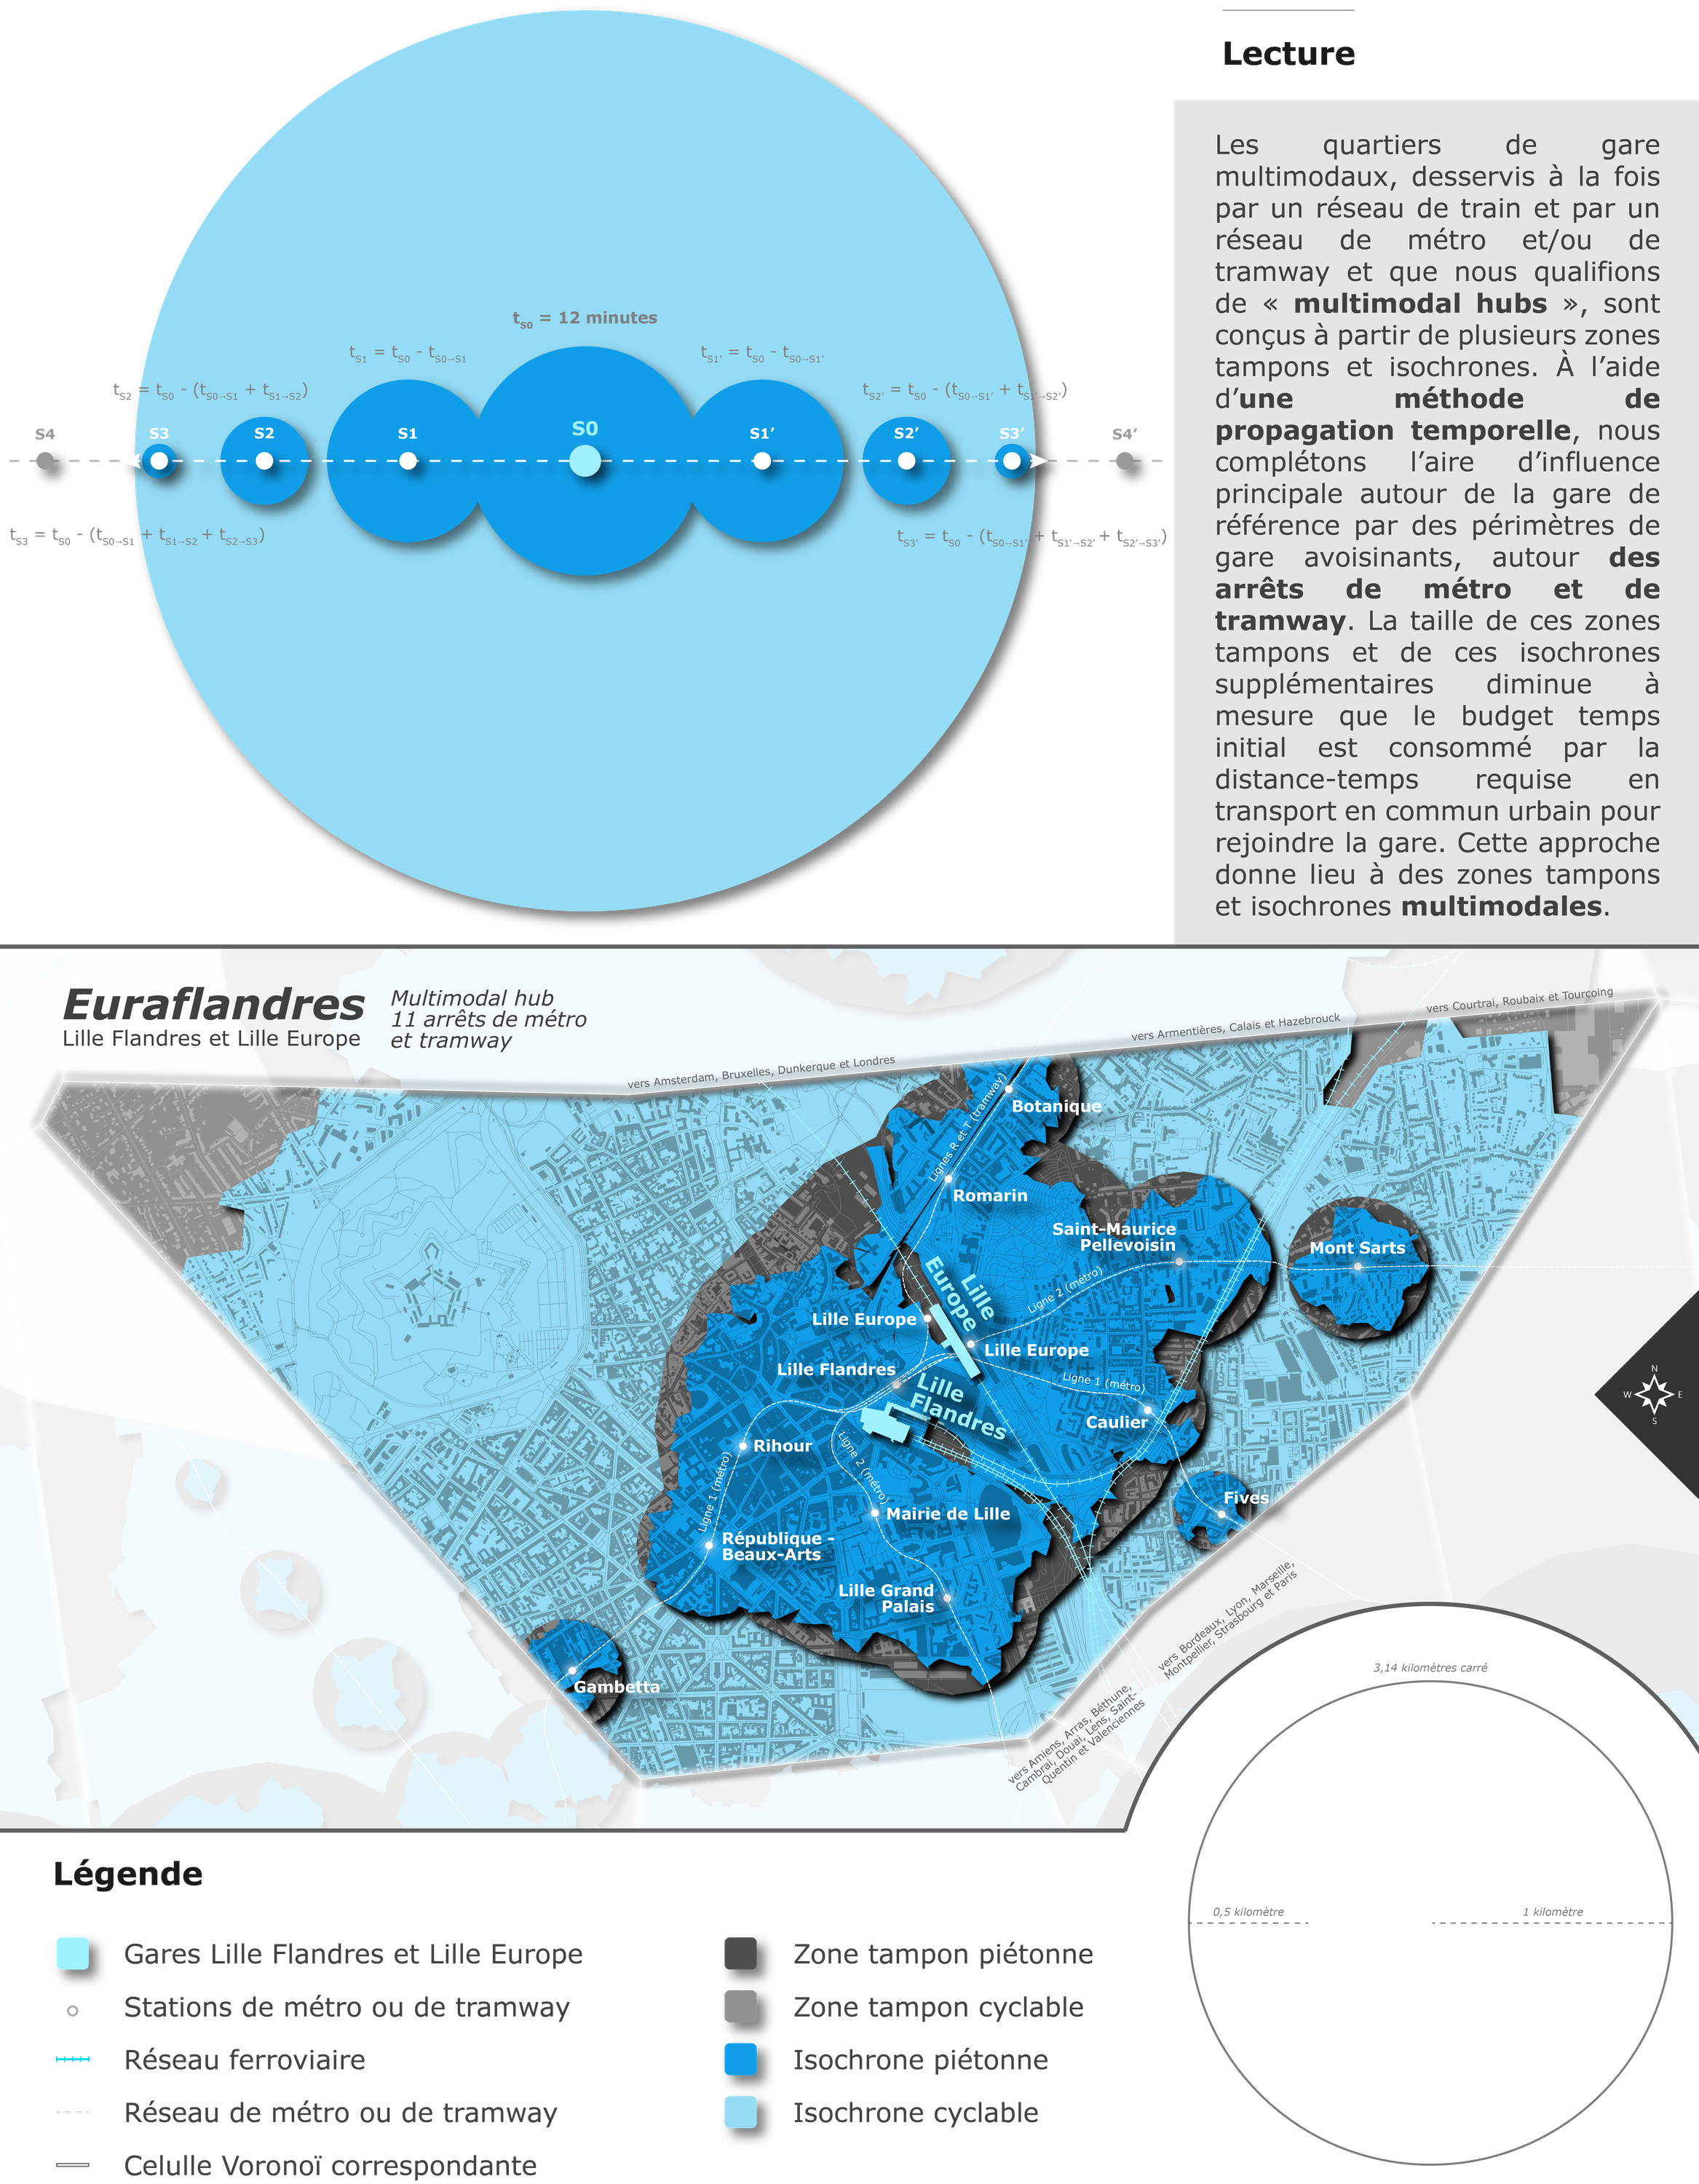
\includegraphics[width=1\columnwidth]{src/Figures/Chap-3/FR_Carte_Euraflandres.png}}
        \vspace{5pt}
        \begin{flushright}\scriptsize{
        Jeux de données~: \textcolor{blue}{\textcite{openstreetmap_openstreetmap_2023}} et \acrshort{GTFS} de la \textcolor{blue}{\textcite{sncf_reseau_2024}}\index{SNCF@\textsl{SNCF}|pagebf}
        \\
        Auteur~: \textcolor{blue}{Dylan Moinse (2024)}
        }\end{flushright}
    \end{carte}

    % OTP
Pour mettre en œuvre cette approche, nous avons utilisé l’outil de génération d’isochrones multimodales du projet \textsl{open-source} \Marque{OpenTripPlanner} (OTP). Ce support permet de calculer des zones accessibles à partir d’un point donné en tenant compte de différents modes de déplacement ainsi que des combinaisons possibles entre ces modes \textcolor{blue}{\autocite[15]{krismer_enhancing_2017}}\index{Krismer, Nikolaus|pagebf}, autant de paramètres qu'il est possible d'ajuster. En mobilisant le module \Guillemets{\textsl{OTP Analyst}}, nous avons pu générer des isochrones représentant les quartiers de gare basés sur leurs connexions multimodales. Au total, 5 gares de la région ont vu leurs aires d’influence étendues à l’ensemble de l'approche multimodale, en raison de leur proximité immédiate avec des stations de métro ou de tramway~: \textsl{Euraflandres}\footnote{
    Nous définissons le pôle \textsl{Euraflandres} à partir d'une fusion entre les gares Lille Flandres et Lille Europe (voir la \hyperref[chap3:observation-quantitative-gares-examinees]{sous-section sur les gares examinées}, page~\pageref{chap3:observation-quantitative-gares-examinees}).
}, Lille CHR, Roubaix, Tourcoing et Valenciennes. Ces pôles d’échange multimodaux ont été désignés sous le terme de \Guillemets{pôles d'échange multimodal} (\textsl{multimodal hubs}). En parallèle, 13 autres gares appartiennent à une seconde catégorie, associée à une desserte en \acrshort{TGV}, tandis qu’une troisième catégorie regroupe un total de 300 gares exclusivement desservies par le \acrshort{TER}.%%Rédigé%%

    % Transition
Compte tenu du nombre important de nœuds que nous étudions au sein du réseau ferroviaire régional, une préoccupation légitime s'élève quant à notre démarche visant à étendre les quartiers de gare à pied comme à vélo et en micro-mobilité~: celle d'une redondance territoriale dans les analyses spatiales, résultant d'une imbrication exagérée des quartiers de gare, notamment dans certaines agglomérations caractérisées par une densité élevée de gares. Face à ce constat, nous proposons de conjuguer la définition des quartiers de gare~–~en modulant leur taille selon le mode de transfert et le type de desserte ferroviaire~–~avec une partition en motifs polygonaux servant à circonscrire chaque quartier de gare.%%Rédigé%%

    % 3.2.1.3.
    \needspace{1\baselineskip} % Réserve de l'espace
\subsubsection*{Délimitation par juxtaposition des quartiers de gare
    \label{chap3:quartiers-gare-voronoi}
    }

    % Superposition
Une dernière préoccupation concernant la problématique de la taille des quartiers de gare réside dans la question de la superposition des aires d'influence ainsi représentées. Si, dans le cas d’un système ferroviaire, la distance inter-station est généralement importante, l’extension des quartiers de gare entreprise par le biais de l’intégration de la mobilité individuelle légère soulève légitimement la question d’une surabondance d’aires superposées. Ce problème ne se limite pas tant à une simple question d'esthétique ou de lisibilité cartographique, mais concerne également le risque de répétition analytique excessive des mêmes configurations territoriales. À titre d’illustration, l’aire d’influence \Guillemets{secondaire} de la gare de La Madeleine, sans bornage, englobe en son sein les gares Lille Flandres et Lille Europe, ce qui fausse grandement les scores de la gare périphérique.%%Rédigé%%

    % Diagramme de Voronoi
Dans la mesure où nous supposons que les utilisateur·rice·s de la mobilité individuelle légère, entrant ou sortant d'une gare, cherchent à emprunter le chemin le plus court \textcolor{blue}{\autocite[116]{heran_distances_2009}}\index{Héran, Frédéric|pagebf}, nous avons opté pour une partition du réseau ferroviaire régional afin de définir les espaces théoriquement les plus proches, d'un point de vue géométrique, de chaque station. Ce découpage, basé sur un plan euclidien, permet de modéliser et de visualiser la couverture théorique maximale de chaque aire d'influence, représentée par une cellule issue d’un diagramme standard de Voronoï \textcolor{blue}{\autocite[479]{mota_method_2014}}\index{Mota, Diego Rosa|pagebf}\index{Takano, Marise|pagebf}\index{Taco, Pastor Willy Gonzales|pagebf}. Cette approche consistant à éviter toute forme de superposition revient à considérer que chaque cellule correspond à un espace dans lequel tous les points sont plus proches de la gare associée qu’à toute autre gare, et ce, indépendamment de la hiérarchie du réseau ferroviaire \textcolor{blue}{\autocite[429]{lebedeva_increasing_2018}}\index{Lebedeva, Olga|pagebf}\index{Kripak, Marina|pagebf}\index{Gozbenko, Valeriy|pagebf}.%%Rédigé%%

    % Transition
Pour représenter le périmètre géographique des 318 gares composant le réseau ferroviaire des Hauts-de-France, notre analyse s’est d’abord focalisée sur la détermination de la taille des différentes aires de chalandise. Cette démarche a consisté à distinguer, dans un premier temps, les quartiers de gare limités à la portée acceptable de la marche combinée, de ceux élargis par l’usage du vélo et de la micro-mobilité. Par la suite, une différenciation a été opérée entre les gares connectées au réseau \acrshort{TER}, celles reliées au réseau \acrshort{TGV}, et les pôles d'échange multimodal. Enfin, un confinement du rayonnement maximal de chaque nœud de transport en commun a été établi, de sorte à le délimiter au sein de frontières. La spatialisation des quatre types de quartier de gare au sein du réseau régional peut être visualisée sur la \hyperref[fig-chap5:aires-influence]{carte~\ref{fig-chap5:aires-influence}} (page~\pageref{fig-chap5:aires-influence}) du \hyperref[chap5:titre]{chapitre~5} (page~\pageref{chap5:titre}). Une fois les tailles définies et intégrées dans le protocole méthodologique, notre attention se porte désormais sur la morphologie que prennent ces quartiers de gare, et notamment aux formes qu'ils peuvent adopter et aux manières de les représenter.%%Rédigé%%

    % 3.2.2.
    \needspace{1\baselineskip} % Réserve de l'espace
\subsection{Morphologie et contours des quartiers de gare
    \label{chap3:quartiers-gare-formes}
    }

    % Introduction
La question de la forme des quartiers de gare semble, à notre connaissance, bien moins explorée dans la littérature scientifique et technique. Cela peut s'expliquer par la complexité qu’elle revêt, tant au niveau des structures territoriales que des considérations techniques, nécessitant une maîtrise avancée des outils permettant de générer divers types d’aires d’influence. Si le sujet des zones tampons, de leurs limitations, ainsi que de l’intérêt d’adopter des isochrones, voire de les combiner pour en tirer une synergie intéressante, est relativement bien documenté, la discussion autour de leur rendu et de leur représentation reste encore critique. C’est dans cette sous-section que nous définissons deux formes de quartier de gare~–~les zones tampons (\(B\)) et les courbes isochrones (\(I\))~–~qui viennent s’ajouter à la réflexion sur la taille de leurs périmètres (\(P\) et \(B\)). Pour autant, leur visualisation demeure un enjeu central. Pour cette raison, nous avons choisi d’approfondir la réflexion sur les différentes manières de représenter ces quartiers, dans le but de développer une démarche méthodologique permettant de concevoir nos propres zones tampons et isochrones. Ce cheminement de pensée cartographique s’appuyant sur une combinaison de techniques informatiques et visuelles.%%Rédigé%%

    % 3.2.2.1.
    \needspace{1\baselineskip} % Réserve de l'espace
\subsubsection*{Intégration des effets de coupure urbaine
    \label{chap3:quartiers-gare-isochrones-buffers}
    }

    % Buffers
Encore aujourd’hui, la majorité des études, qu’elles soient académiques ou opérationnelles, s’appuient sur l'exploitation de disques théoriques (\textsl{buffers}) pour représenter les aires de chalandise des stations de transport en commun. Ces zones tampons se traduisent par des cercles tracés à une distance fixe, qu’elle soit spatiale ou temporelle, autour des nœuds de transport, et ce, sans considération des réseaux ou des obstacles géographiques environnants. Cette méthode présente l’avantage d’être simple à produire et facile à interpréter, puisqu’elle ne nécessite ni données complexes ni calculs avancés. Elle offre également une grande polyvalence, pouvant être appliquée à différents types d’infrastructures, même au-delà des enjeux strictement liés à la mobilité. Cependant, cette technique de production des quartiers de gare se heurte à des limitations majeures. En s’appuyant sur une représentation des distances à vol d’oiseau, sur un plan euclidien, elle ignore les réseaux de transport ainsi que les contraintes géographiques de l'environnement physique. Par conséquent, les zones tampons ne traduisent pas l’accessibilité réelle des infrastructures. Une telle simplification peut conduire à des conclusions inexactes, particulièrement dans des contextes où la configuration des réseaux et des territoires joue un rôle déterminant dans la définition des quartiers de gare.%%Rédigé%%

    % Effets de coupure urbaine
La problématique du redressement des distances à vol d’oiseau pour obtenir des distances réelles n’est pas seulement technique. Elle impose une réflexion sur les effets de coupure urbaine, ainsi qu’une interrogation sur l’origine des détours, impliquant ainsi une analyse de la configuration du réseau viaire, de son maillage et de sa hiérarchisation \textcolor{blue}{\autocite[119]{heran_distances_2009}}\index{Héran, Frédéric|pagebf}. Une coupure urbaine se définit comme une emprise perturbant les relations entre les populations environnantes. Cette emprise peut être d’origine naturelle ou artificielle, bâtie ou non bâtie. L’effet de coupure urbaine se manifeste par des emprises linéaires ou surfaciques, engendrant des perturbations d’ordre physique ou psychologique \textcolor{blue}{\autocite[4]{heran_zones_2009}}\index{Héran, Frédéric|pagebf}\index{Pouillaude, Laurence|pagebf}. Parmi les effets de coupure urbaine les plus emblématiques figurent les autoroutes ou les formes urbaines, ainsi que les fleuves ou les montagnes. Paradoxalement, les infrastructures ferroviaires elles-mêmes peuvent contribuer à ces effets de coupure. Le rapport de recherche-action franco-allemand \textsl{Bahn.Ville 2} illustre cette problématique en montrant comment les voies ferrées participent dans la production de coupures urbaines, renforçant ainsi une \gls{perception} négative, voire une invisibilité, du rail dans l’espace urbain \textcolor{blue}{\autocite[20]{lhostis_concevoir_2009}}\index{L'Hostis, Alain|pagebf}\index{Alexandre, Elsa|pagebf}\index{Appert, Manuel|pagebf}\index{Araud-Ruyant, Catherine|pagebf}\index{Basty, Marius|pagebf}\index{Biau, Géraldine|pagebf}\index{Bozzani-Franc, Sandra|pagebf}\index{Boutantin, Gratienne|pagebf}\index{Constantin, Chantal|pagebf}\index{Coralli, Monica|pagebf}\index{Durousset, Marie-Jeanne|pagebf}\index{Fradier, Christophe|pagebf}\index{Gabion, Cyrille|pagebf}\index{Leysens, Thomas|pagebf}\index{Mermoud, Françoise|pagebf}\index{Olny, Xavier|pagebf}\index{Perrin, Emmanuel|pagebf}\index{Robert, Jean|pagebf}\index{Simand, Noémie|pagebf}\index{Stransky, Vaclav|pagebf}\index{Soulas, Claude|pagebf}\index{Verdier, Anne-Marie|pagebf}\index{Vulturescu, Bogdan|pagebf}. Dès lors, la coupure urbaine constitue un élément important pour comprendre les interactions entre le système ferroviaire et les territoires.%%Rédigé%%

    % Isochrones
C’est dans cette optique que les isochrones sont fréquemment considérées comme une représentation plus réaliste des zones accessibles. Contrairement aux zones tampons, elles délimitent les espaces atteignables dans un temps donné, à partir ou à destination d’une gare, tout en intégrant les infrastructures et les modes de déplacement. En prenant en compte le réseau de voiries ainsi que les spécificités des différents modes de déplacement~–~principalement leur rayon d'action, leur vitesse et les zones qu'ils sont habilités à traverser~–, les isochrones offrent une représentation plus fidèle de l’accessibilité. Par sa capacité à refléter les dynamiques spatiales réelles, la modélisation d'isochrones constitue un outil d'évaluation précise des zones effectivement accessibles. Les premières occurrences dans le champ de la géographie datent du début du XX\textsuperscript{e} siècle, à l'image des \Guillemets{lignes isochrones}, dessinées par \textcolor{blue}{Joseph} \textcolor{blue}{\textcite[311-314]{letaconnoux_note_1907}}\index{Letaconnoux, Joseph|pagebf}, sur l'évolution de l'accessibilité en Bretagne depuis le XVIII\textsuperscript{e} siècle. Dans le domaine de l'urbanisme, généralement piétonnes, les isochrones trouvent leurs premiers usages dans les travaux de \textcolor{blue}{Jane} \textcolor{blue}{\textcite[179-182]{jacobs_death_1961}}\index{Jacobs, Jane|pagebf} qui a introduit le concept de \Guillemets{bassins d'usage} (\textsl{pools of use}) pour désigner les zones situées à distance de marche d'un emplacement urbain spécifique, en fonction du temps de parcours \textcolor{blue}{\autocite[3]{dovey_isochrone_2017}}\index{Dovey, Kim|pagebf}\index{Woodcock, Ian|pagebf}\index{Pike, Lucinda|pagebf}. À titre d’exemple, la \acrfull{MEL}, anciennement \acrfull{LMCU}, a cartographié, en 2000, des \acrfull{ZAP} et des \acrfull{ZAV} autour de ses stations de transport en commun lourd. Ces courbes isochrones ont été conçues pour identifier les lieux stratégiques de développement métropolitain \textcolor{blue}{\autocite[9]{heran_zones_2009}}\index{Héran, Frédéric|pagebf}\index{Pouillaude, Laurence|pagebf}.%%Rédigé%%
    
    % Isodistances
Dans une logique similaire visant à dépasser l’idée des distances à vol d’oiseau définies par les zones tampons, se trouvent les courbes d’isodistance, souvent confondues avec les isochrones. Pourtant, une distinction fondamentale existe~: les isodistances désignent les zones regroupant tous les points situés à une distance spatiale réelle, mesurée sur un réseau, à partir d’un point de référence tel qu’une station de transport en commun. Tiré du grec \textsl{isos} (égal) et \textsl{khronos} (temps), le terme isochrone se différencie de l’isodistance, qui renvoie à une zone définie par une distance spatiale réelle, déformée par le réseau, mais indépendante des vitesses ou des temps de parcours. L’isodistance illustre ainsi une zone de chalandise isométrique, contrairement à l’isochrone, qui repose sur une distance temporelle. Cette confusion fréquente peut s’expliquer par la prédominance des études d’accessibilité piétonne autour des gares. Ces études supposent souvent que les vitesses relativement homogènes des piéton·ne·s entraînent une superposition des courbes isochrones et des courbes d’isodistance \textcolor{blue}{\autocite[9]{heran_zones_2009}}\index{Héran, Frédéric|pagebf}. Cependant, dans le cas de la mobilité cyclable, ces similarités tendent à s’effacer. Les vitesses bien plus variables de la mobilité individuelle légère, influencées par la hiérarchie viaire, la qualité des aménagements ou encore des facteurs individuels comme le type de véhicule ou les compétences des cyclistes, soulignent le besoin de différencier clairement ces notions.%%Rédigé%%

    % Combinaison isochrones et buffers
Durant le déroulement de nos travaux de thèse, nous avons privilégié l’utilisation conjointe des zones tampons, des isodistances et des isochrones. Leur combinaison dans l’analyse spatiale fournit une perspective intégrée sur l’accessibilité. En superposant les isodistances ou les isochrones et les zones tampons, il devient possible de mesurer les différentiels d’accessibilité, c’est-à-dire l’écart entre l’accessibilité réelle et l’accessibilité théorique. Cette confrontation permet en outre de calculer le taux de desserte qui exprime le rapport entre l’aire réellement accessible et l’aire atteignable en ligne droite \textcolor{blue}{\autocite[13]{heran_zones_2009}}\index{Héran, Frédéric|pagebf}. Le diagnostic cartographique de ces différentes représentations de quartiers de gare permet d’identifier de manière systématique les obstacles rencontrés par les voyageur·se·s.%%Rédigé%%

    % Transition
Une fois le débat sur les apports des isochrones dépassé~–~une étape nécessaire, mais qui semble, d’après nos observations, de plus en plus admise et couramment intégrée dans diverses productions~–~se pose la question de leur représentation. Bien que les avantages des isochrones, notamment pour intégrer les obstacles physiques présents dans les territoires, soient largement reconnus dans les pratiques de recherche, il apparaît que leur rendu varie considérablement et manque souvent de transparence quant aux paramètres mobilisés. Cette opacité peut s'expliquer par le fait que la plupart d'entre elles sont générées à l’aide de plates-formes limitant la maîtrise des paramètres de modélisation. Face à ce constat, nous avons entrepris de développer nos propres quartiers de gare à l’aide d’un script sur-mesure, nous offrant ainsi la possibilité de définir des délimitations géographiques adaptées à nos objectifs de recherche.%%Rédigé%%

    % 3.2.2.2.
    \needspace{1\baselineskip} % Réserve de l'espace
\subsubsection*{Réflexion à propos de la représentation cartographique des quartiers de gare
    \label{chap3:quartiers-gare-python}
    }

% Fabrique des aires d'influence : Python (précision géographique)
Une réflexion approfondie s’impose pour établir les stratégies de représentation cartographique des zones d’accessibilité, telles que les zones tampons et les isochrones, en adéquation avec les objectifs de cette recherche doctorale. Cette démarche ne relève pas uniquement de considérations esthétiques ou de communication, mais vise également à assurer une maîtrise, tant sur le fond que sur la forme, des bases d’analyse géographique mobilisées tout au long de ce travail. Il convient, en premier lieu, de clarifier les concepts abordés, notamment en identifiant les paramètres qui influencent la configuration des représentations et les interprétations analytiques qui en découlent. Face à la diversité des outils disponibles pour la génération des zones tampons et des isochrones, nous avons opté pour la poursuite de notre analyse à l’aide du langage de programmation \textsl{Python}. Ce choix repose non seulement sur la richesse des bibliothèques proposées par cet environnement, mais également sur la transparence offerte par l’outil en source ouverte (\textsl{open source}) qui autorise une maîtrise totale des paramètres définis\footnote{
    \textsl{Python} est un langage généraliste et applicable à de larges domaines qui devient de plus en plus populaire auprès des \textsl{data scientists} \textcolor{blue}{\autocite[19]{velt_python_2020}}\index{Velt, Amandine|pagebf}. En plus de sa documentation très fournie, \textsl{Python} dispose d'une interface graphique pour l'analyse des données et du partage des analyses~: les \textsl{notebooks Jupyter}. Un \textsl{notebook} est un document exécutable dont les résultats sont intégrés dans le document, en plus d'éléments de texte ou d'équations mathématiques. Dès lors, l'outil \textsl{Jupyter Notebook} et l'usage de \textsl{Python}, accompagnés de bibliothèques utiles telles que \textsl{Pandas} et \textsl{GeoPandas}, ont été généralisés dans nos analyses afin d'assurer une plus grande transparence et une meilleure gestion du travail en équipe \textcolor{blue}{\autocite[55, 137]{velt_python_2020}}\index{Velt, Amandine|pagebf}.
}.%%Rédigé%%

    % Isochrone depuis et vers
Un premier paramètre qui vient interroger la fabrique géographique des aires d’influence des gares réside dans le sens des flux. À première vue, il pourrait sembler intuitif de considérer que, quelle que soit la direction du flux~–~qu’il s’agisse d'un trajet en rabattement vers la gare ou en diffusion depuis celle-ci~–, le quartier de gare conserverait une taille et une forme similaires. Cependant, cette hypothèse tend à négliger deux dimensions~: la connectivité routière, particulièrement déterminante pour le vélo et la micro-mobilité, qui sont régis par les contraintes du code de la route, ainsi que la temporalité. En effet, une isochrone orientée vers ou depuis une gare ne possède pas nécessairement la même validité selon des facteurs tels que l’amplitude horaire des lignes ou les directions desservies. S'agissant de notre matériau empirique, nous avons choisi de considérer que, par défaut, les zones tampons et les isochrones atemporelles sont conçues pour analyser les aires accessibles en direction de la gare, et non dans l’autre sens, comme cela est souvent le cas. Ce choix s'explique par la primauté de la logique de pré-acheminement, qui est privilégiée dans la mesure où le vélo, lorsqu'il est utilisé en connexion avec les gares, y est bien plus sollicité qu'en post-acheminement.%%Rédigé%%

    % Surface VS voirie VS bâti VS POIs
La problématique de la représentation cartographique des isochrones, qu’il s’agisse de leur dimension analytique ou de leur fonction communicative, se pose également en termes de choix des éléments structurants à mettre en avant. Faut-il privilégier une représentation visuelle de la surface accessible ou non accessible~? Ou bien serait-il plus pertinent de mettre en exergue la voirie, qui matérialise les connexions servant de base au calcul de l’isochrone~? Une autre possibilité consisterait à mettre l'accent sur le bâti ou les \acrfull{POIs}, qui incarnent, en définitive, les destinations que les individus cherchent à atteindre. Ces choix cartographiques ne sont pas neutres, car ils orientent la lecture et l’interprétation des données tout en influençant la manière dont les résultats sont communiqués aux divers publics concernés.%%Rédigé%%

    % Isochrone voirie
La représentation basée sur la voirie reflète directement les trajets réalisables au sein d’un réseau piétonnier ou cyclable défini. Ce mode de visualisation prétend offrir une approche plus réaliste en prenant en compte les contraintes physiques des déplacements, tout en étant particulièrement adaptée à la navigation et aux repères cartographiques\footnote{
    L'\acrfull{API} la plus connue pour la création d’isochrones basées sur la voirie est certainement celle développée par \textcolor{blue}{\textcite{graphhopper_visualization_2018}}.
}. Cependant, une telle représentation peut également engendrer une certaine complexité visuelle, rendant l’interprétation plus difficile pour certain·e·s utilisateur·rice·s. Au-delà des simples polygones, celle-ci propose une représentation détaillée des segments de voies accessibles, directement visualisables dans un navigateur. À titre illustratif, nous avons appliqué cette méthode, avec notre propre code, pour représenter, en projection plane et en modèle volumétrique, l’isochrone accessible en mobilité individuelle légère à destination de la gare d’Amiens. Cette représentation repose sur la voirie directement accessible aux cyclistes (voir la \hyperref[fig-chap3:isochrone-amiens-voirie]{carte~\ref{fig-chap3:isochrone-amiens-voirie}}, page~\pageref{fig-chap3:isochrone-amiens-voirie})\footnote{
    Cette analyse cartographique a été améliorée grâce à l’utilisation de la transparence des couleurs, qui met en relief les matrices de flux. L’efficacité de cette technique combinée à un fond sombre réside dans l’optimisation de la \Guillemets{saillance visuelle}~–~cette notion fait référence à l’adéquation entre le phénomène représenté, les variables visuelles utilisées et leur perception par l’observateur·rice~–~des éléments représentés et des informations transmises, tout en facilitant la perception des géométries complexes. Cette approche garantit une lisibilité accrue, comme le démontre \textcolor{blue}{Françoise} \textcolor{blue}{\textcite[226]{bahoken_contribution_2016}}\index{Bahoken, Françoise|pagebf}, dans sa thèse de doctorat, sur la base d'une cartographie d’une matrice de flux.
}.%%Rédigé%%

    % Carte Isochrone Amiens voirie
    \begin{carte}[h!]\vspace*{4pt}
        \caption{Représentation cartographique du réseau viaire atteignable à vélo et en micro-mobilité vers la gare d'Amiens, construite à partir d'une isochrone.}
        \label{fig-chap3:isochrone-amiens-voirie}
        \centerline{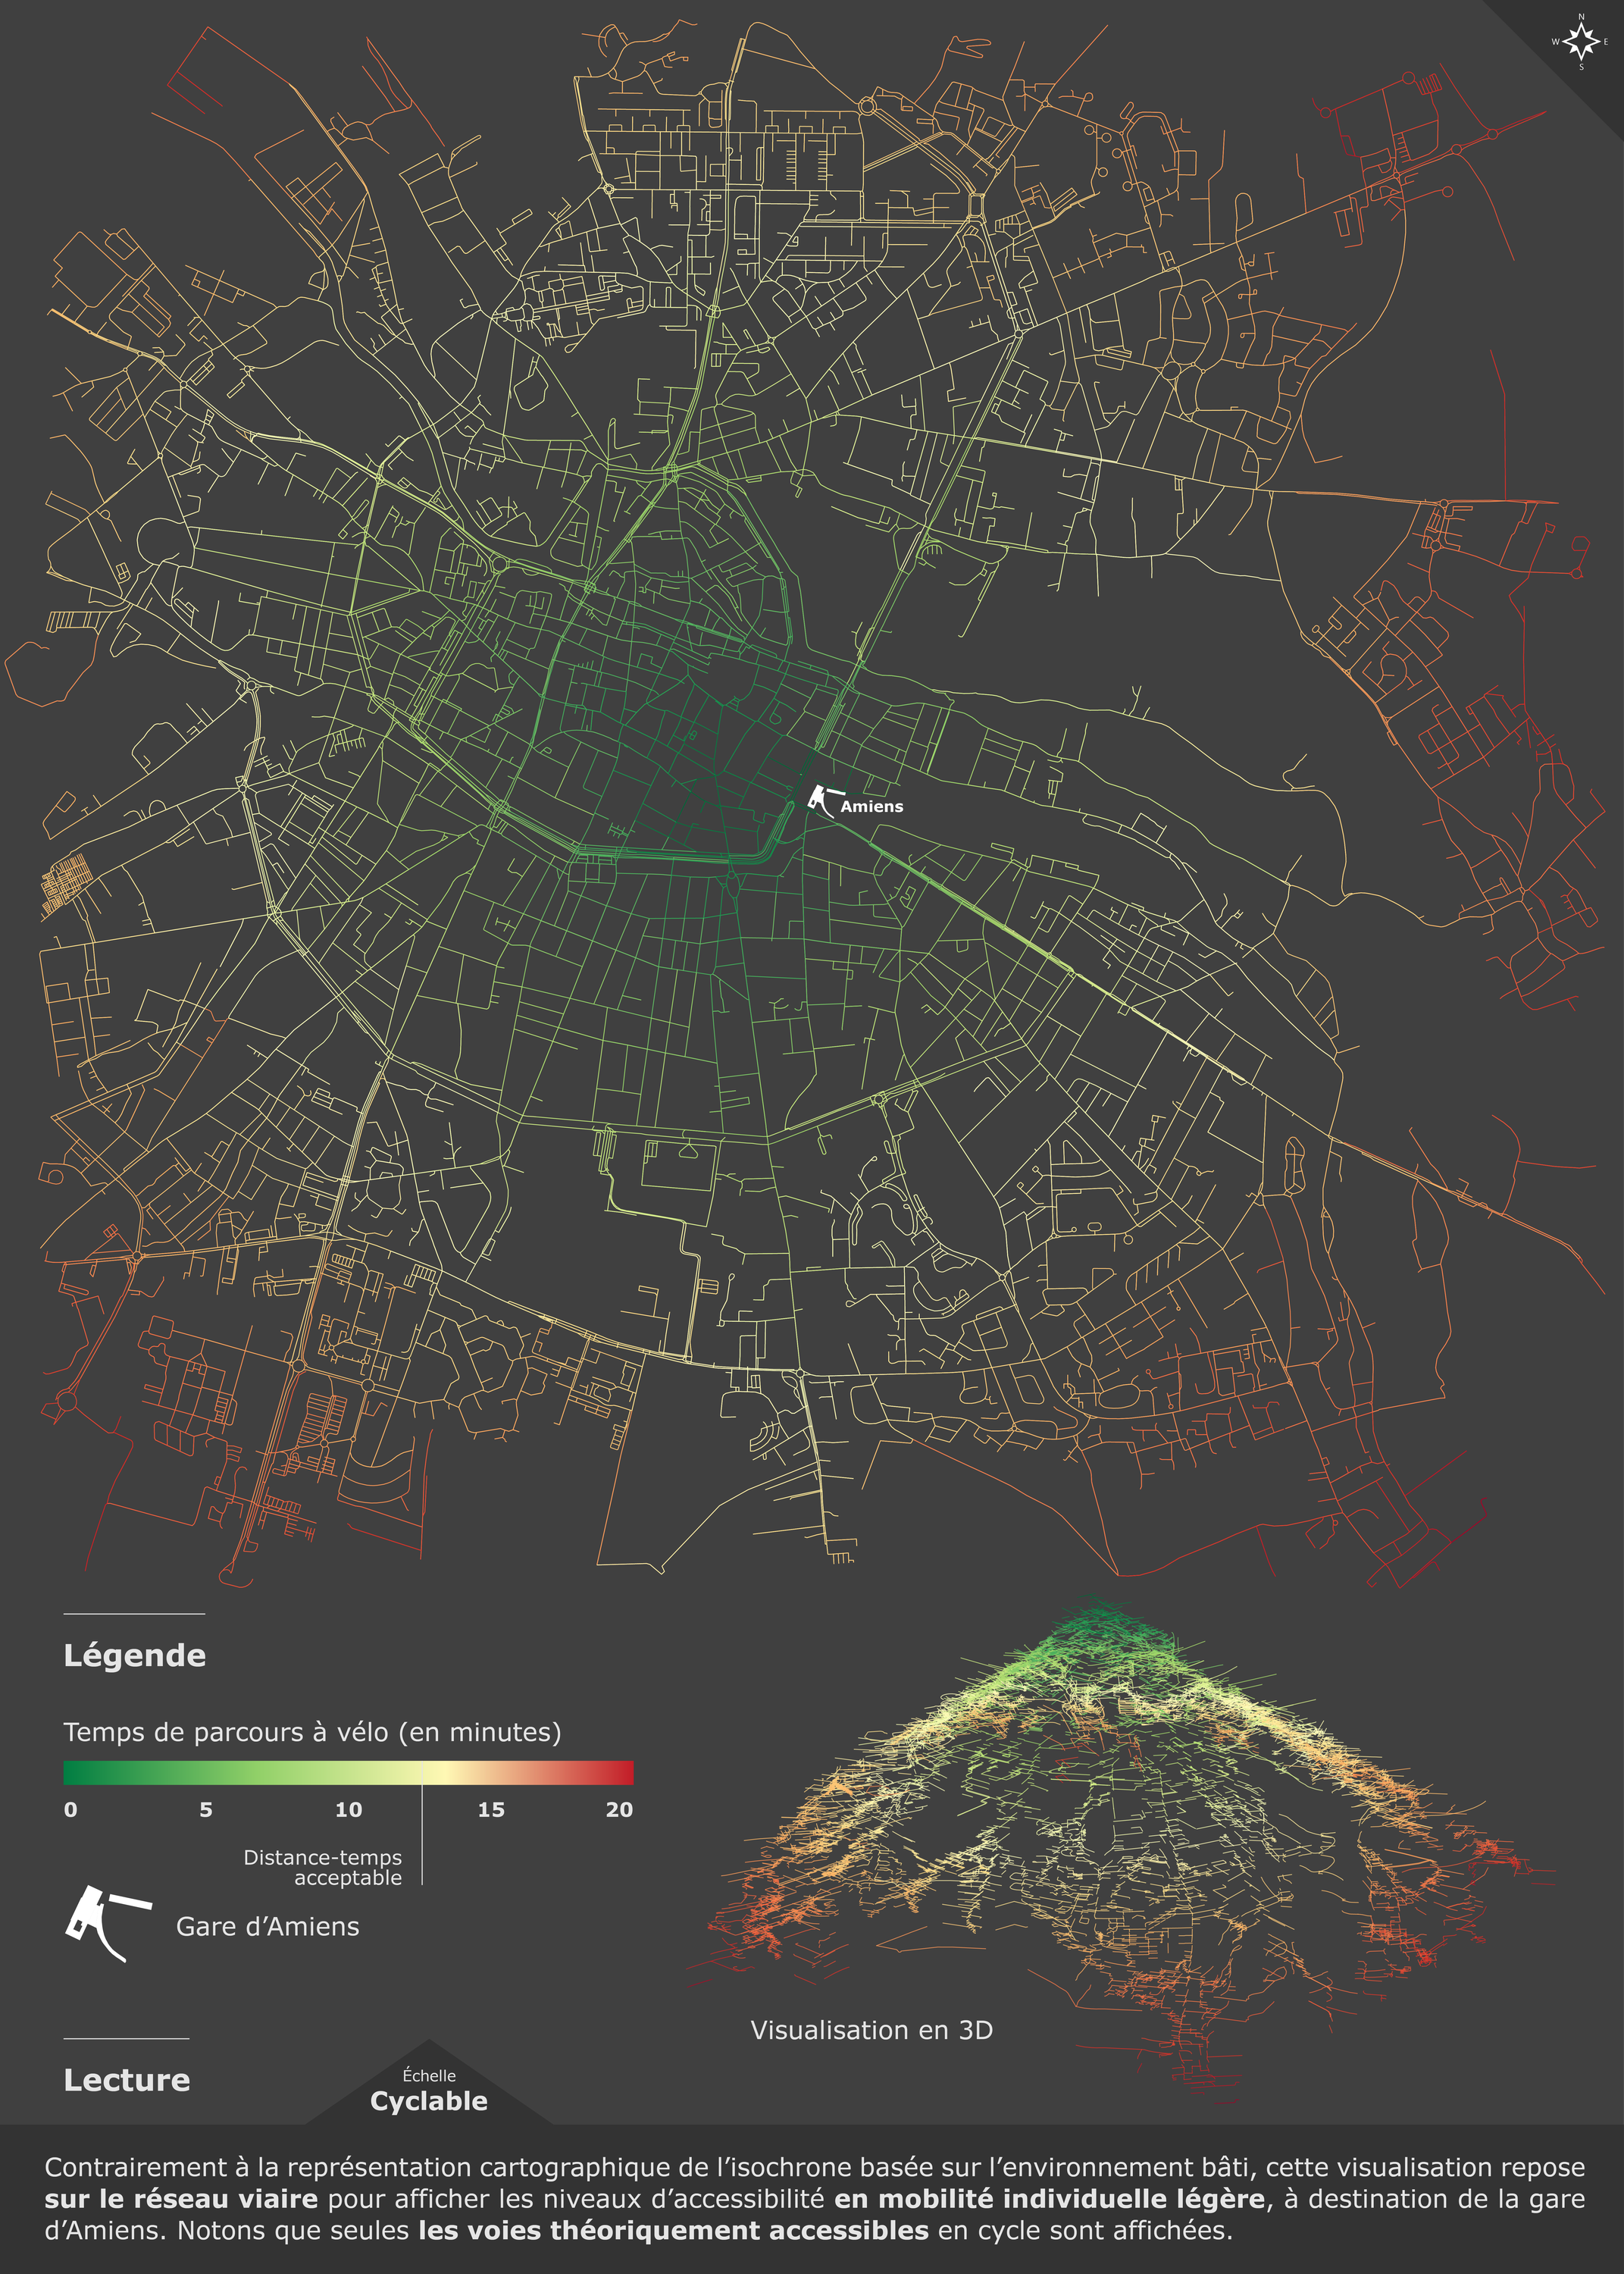
\includegraphics[width=1\columnwidth]{src/Figures/Chap-3/FR_Carte_Isochrone_Amiens_Voirie.png}}
        \vspace{5pt}
        \begin{flushright}\scriptsize{
        Jeux de données~: \textcolor{blue}{\textcite{openstreetmap_openstreetmap_2023}} et \acrshort{GTFS} de la \textcolor{blue}{\textcite{sncf_reseau_2024}}\index{SNCF@\textsl{SNCF}|pagebf}
        \\
        Auteur~: \textcolor{blue}{Dylan Moinse (2024)}
        }\end{flushright}
    \end{carte}

    % Isochrone bâti
En ce qui concerne la représentation basée sur le bâti ou les \acrshort{POIs} accessibles dans le temps imparti, elle présente l’avantage de mieux répondre aux besoins des utilisateur·rice·s en orientant le regard vers les lieux où les individus interagissent directement, tels que les logements, les lieux de travail, les commerces ou encore les équipements publics (voir la \hyperref[fig-chap3:isochrone-amiens-bati]{carte~\ref{fig-chap3:isochrone-amiens-bati}}, page~\pageref{fig-chap3:isochrone-amiens-bati}). Cette approche est particulièrement pertinente pour des analyses centrées sur des services spécifiques, en fournissant une réponse immédiate et pratique à la question de l'accessibilité aux services. Cependant, cette forme de représentation visuelle présente certaines limites. Elle exclut les zones non bâties, qui expriment pourtant un besoin en matière d'accessibilité, comme les espaces verts ou d’autres espaces ouverts ayant une valeur fonctionnelle ou sociale. De plus, elle ne permet pas de mettre en évidence la connectivité globale de la zone.%%Rédigé%%

    % Carte Isochrone Amiens bâti
    \begin{carte}[h!]\vspace*{4pt}
        \caption{Représentation cartographique du bâti atteignable à vélo et en micro-mobilité vers la gare d'Amiens, construite à partir d'une isochrone.}
        \label{fig-chap3:isochrone-amiens-bati}
        \centerline{\includegraphics[width=1\columnwidth]{src/Figures/Chap-3/FR_Carte_Isochrone_Amiens_Bati.png}}
        \vspace{5pt}
        \begin{flushright}\scriptsize{
        Jeux de données~: \textcolor{blue}{\textcite{openstreetmap_openstreetmap_2023}} et \acrshort{GTFS} de la \textcolor{blue}{\textcite{sncf_reseau_2024}}\index{SNCF@\textsl{SNCF}|pagebf}
        \\
        Auteur~: \textcolor{blue}{Dylan Moinse (2024)}
        }\end{flushright}
    \end{carte}

    % Avantages et inconvénients types d'isochrones
Sur un mode comparatif, nous pouvons établir que les isochrones, traditionnellement représentées sous forme de surfaces accessibles, offrent l’avantage d’une grande clarté visuelle, requièrent généralement un volume limité de données géographiques et sont adaptées à des analyses globales. Contrairement à la représentation par la voirie, bien que plus précise, qui s’adresse davantage à des usages spécifiques tels que la navigation, moins pertinents dans le cadre de notre problématique de recherche. Finalement, les représentations fondées sur l’environnement bâti ou sur les équipements et services accessibles dans un territoire ont le mérite de proposer une orientation davantage centrée sur le·la voyageur·se. Elles se prêtent bien aux analyses urbanistiques, notamment au sujet des formes urbaines et de l’accessibilité aux services ciblés. Toutefois, ce type de représentation cartographique est plus exigeant en termes de données et implique des coûts de \gls{cartographie} plus élevés.%%Rédigé%%

    % Isochrone finale : jeu sur les arêtes
Dans cette perspective, nous avons choisi de croiser les formes de représentation cartographique auxquelles nous nous sommes essayé·e·s, en nous appuyant sur la production d’isochrones hybrides~: surfaciques, certes, mais dont la forme dépend en premier lieu du réseau viaire tout en étant influencée par la présence du bâti environnant (voir la \hyperref[fig-chap3:isochrone-amiens-finale]{carte~\ref{fig-chap3:isochrone-amiens-finale}}, page~\pageref{fig-chap3:isochrone-amiens-finale}). L'adoption de cette technique nous a permis de produire des représentations cartographiques aux contours nettement plus précis que les approximations souvent observées dans les productions traditionnelles d’isochrones. Dans cette démarche, nous nous sommes appuyé·e·s sur la méthode novatrice développée par le développeur logiciel et chercheur \textcolor{blue}{Kuan} \textcolor{blue}{\textcite{butts_better_2017}}\index{Butts, Kuan|pagebf}, reposant sur l’outil \textsl{OSMnx}, disponible en langage de programmation \textsl{Python}, et spécifiquement conçu pour modéliser les réseaux viaires \textcolor{blue}{\autocite[132]{boeing_osmnx_2017}}\index{Boeing, Geoff|pagebf}. Cette approche s’inscrit dans l’esprit d’une carte d’isochrones construite sur la base de la voirie (\textsl{lines}), en adoptant une logique de graphes de réseaux (\textsl{edges}), tout en intégrant une zone tampon linéaire autour de chaque voie et de chaque intersection accessible (\textsl{buffers}). Ce procédé permet dès lors d’incorporer les éléments urbains adjacents au réseau viaire \textcolor{blue}{\autocite[135]{boeing_osmnx_2017}}\index{Boeing, Geoff|pagebf}, sans les mobiliser dans la représentation comme dans la \hyperref[fig-chap3:isochrone-amiens-bati]{carte~\ref{fig-chap3:isochrone-amiens-bati}} (page~\pageref{fig-chap3:isochrone-amiens-bati}.%%Rédigé%%

    % Carte Isochrone finale adoptée Amiens
    \begin{carte}[h!]\vspace*{4pt}
        \caption{Représentation cartographique de l'isochrone accessible à vélo et en micro-mobilité vers la gare d'Amiens, en superposition avec le réseau viaire.}
        \label{fig-chap3:isochrone-amiens-finale}
        \centerline{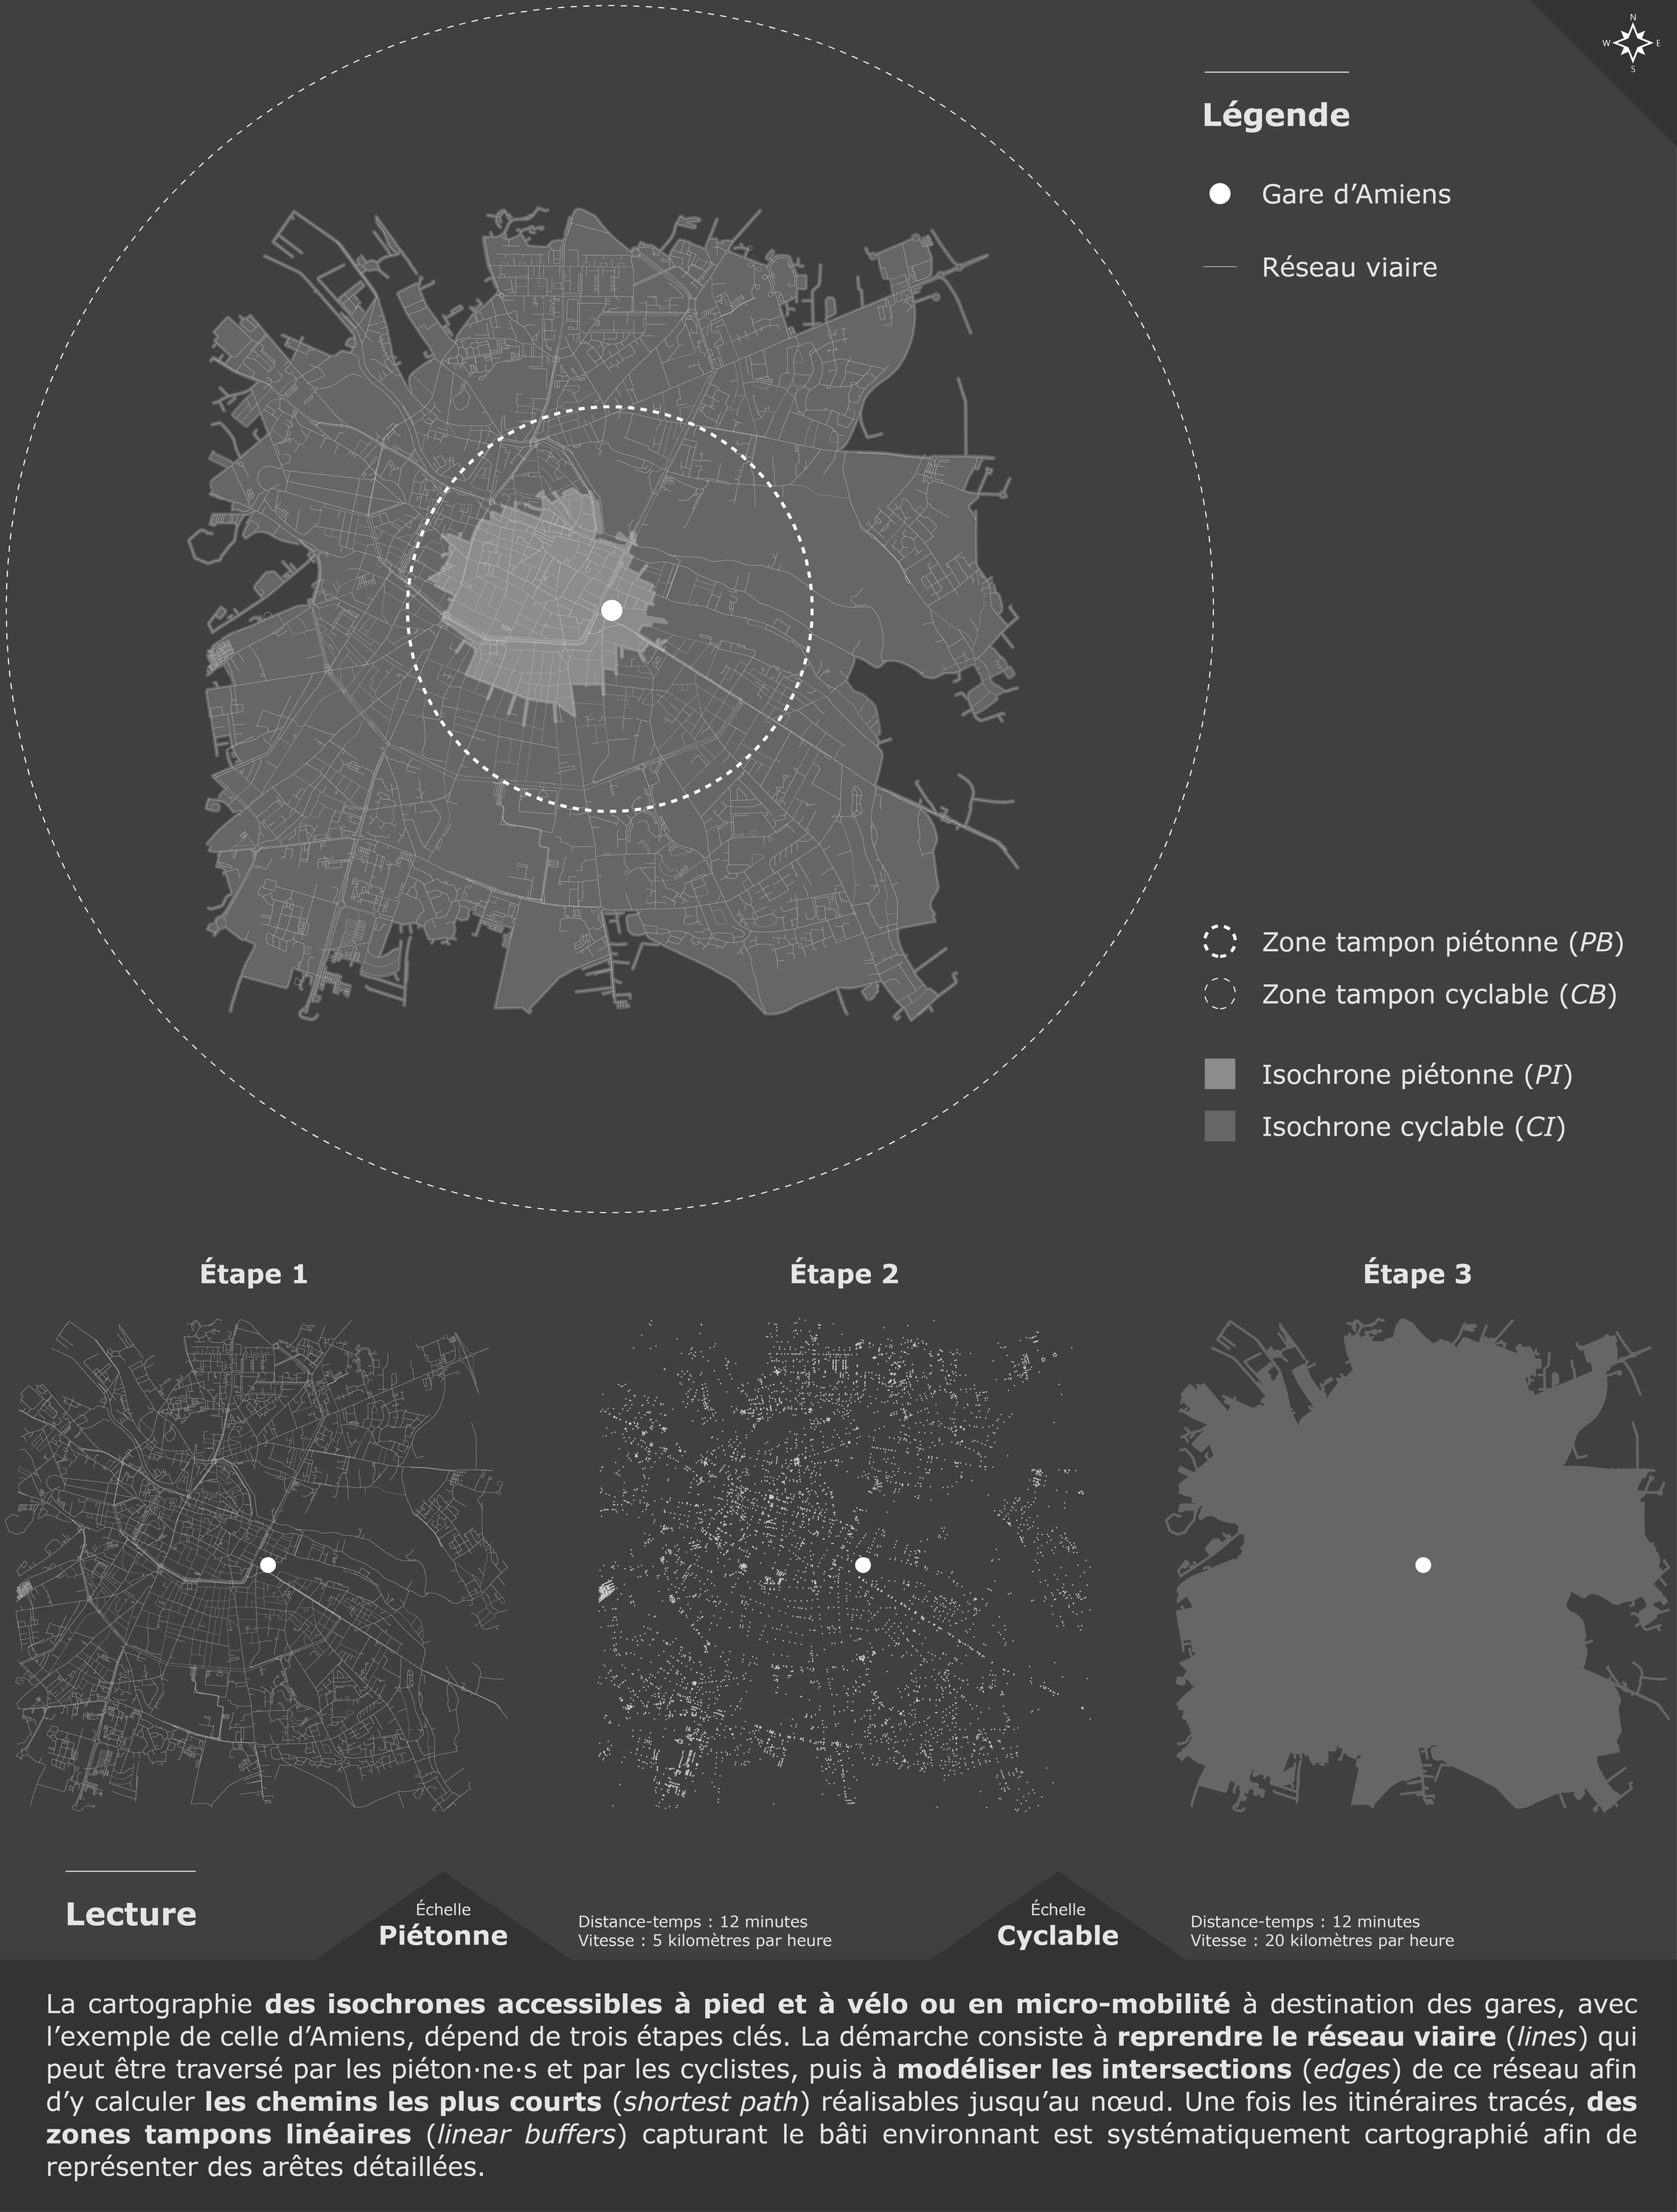
\includegraphics[width=1\columnwidth]{src/Figures/Chap-3/FR_Carte_Isochrones_Buffers_Amiens.png}}
        \vspace{5pt}
        \begin{flushright}\scriptsize{
        Jeux de données~: \textcolor{blue}{\textcite{openstreetmap_openstreetmap_2023}} et \acrshort{GTFS} de la \textcolor{blue}{\textcite{sncf_reseau_2024}}\index{SNCF@\textsl{SNCF}|pagebf}
        \\
        Auteur~: \textcolor{blue}{Dylan Moinse (2024)}
        }\end{flushright}
    \end{carte}

    % Zones accessibles/non accessibles et transition
De nombreux questionnements ont orienté, et pourraient encore orienter, cette sous-section, qui s’attache avant tout à une réflexion globale sur la morphologie des isochrones générées. Par exemple, nous aurions pu également discuter de la hiérarchisation visuelle entre le \textsl{visible} et l’\textsl{invisible}. Si l’objectif est de valoriser les zones accessibles, ne serait-il pas plus pertinent de colorer ou de masquer les zones non accessibles~? Cela permettrait non seulement de recentrer l’attention sur les espaces accessibles, mais également de libérer visuellement l’espace cartographique pour intégrer des figurés et des éléments complémentaires, sans que ceux-ci soient visuellement perturbés par l’isochrone. Comme le souligne \textcolor{blue}{Jacques} \textcolor{blue}{\textcite[5]{levy_tournant_1999}}\index{Lévy, Jacques|pagebf}~–~dans son ouvrage central \textsl{Le tournant géographique. Penser l'espace pour lire le monde}~–, le processus de délimitation et de différenciation participe à la formation des espaces géographiques. Ce principe, que nous avons brièvement exploré ici, nous conduit désormais à expliciter les techniques de collecte et d’analyse géographiques mobilisées une fois les quartiers de gare~–~en tant que périmètres géographiques privilégiés de notre terrain d'étude~–~définis.%%Rédigé%%

    % 3.2.3.
    \needspace{1\baselineskip} % Réserve de l'espace
\subsection{Analyse géostatistique des quartiers de gare cartographiés
    \label{chap3:quartiers-gare-analyse-geostatistique}
    }

    % Introduction
L'effort consacré à la production géographique de quartiers de gare aux tailles et aux formes variables serait dépourvu de sens si les données qui y sont intégrées étaient agrégées à des échelles trop larges, comme celle de la commune. Se cantonner à de tels périmètres administratifs ne permettrait ni de refléter l’individualité de chaque quartier de gare, ni de saisir les distinctions entre leurs différents types ou les variations internes à chacun d’eux. En soulevant cette problématique, nous avons établi comme règle méthodologique de nous restreindre à des bases de données désagrégées, sous forme de vecteurs ponctuels, linéaires ou polygonaux, indépendants des grilles ou des frontières administratives. Pour autant, en raison de la rareté des données ouvertes disponibles, malgré une position avantageuse de la France grâce à une centralisation volontariste des jeux de données, il demeure parfois nécessaire de recourir à des données agrégées, pour des impératifs d'anonymisation par exemple. Ainsi, dans un second temps, nous proposons une méthode d’estimation des valeurs fondée sur des données agrégées à l’échelle de grilles régulières. Cette approche permet de contourner les limitations tout en conservant une précision analytique suffisante pour les besoins de notre recherche.%%Rédigé%%

    % 3.2.3.1.
    \needspace{1\baselineskip} % Réserve de l'espace
\subsubsection*{Des données spatiales désagrégées
    \label{chap3:quartiers-gare-donnees-desagregees}
    }

    % Données géocodées désagrégées sans limites administratives
L’étude des quartiers de gare délimités dans la région repose intégralement sur l’exploitation de données géographiques désagrégées. Cette approche méthodologique a pour objectif de garantir une robustesse analytique, tout en offrant une granularité suffisante pour explorer les dynamiques locales spécifiques à ces espaces stratégiques. Les données géographiques désagrégées se distinguent alors par leur haut niveau de détail et leur indépendance par rapport aux découpages administratifs ou aux périmètres prédéfinis. Elles se déclinent sous plusieurs formes~: des points, représentant la localisation exacte d’équipements~; ou des polygones détaillés, illustrant des emprises au sol par exemple.

    % Sources de données
Contrairement aux données agrégées, généralement collectées à des échelles larges, les données désagrégées permettent d’analyser les territoires à une échelle micro-locale, voire ultra-locale. L'intérêt d'adopter une lecture détaillée des quartiers de gare, indépendante des limites communales 
\textcolor{blue}{\autocite[7]{moretti_interconnexion_1999}}\index{Moretti, Anna|pagebf}\index{Vacheret, Guy|pagebf}, revêt une importance majeure. Les données mobilisées dans notre étude proviennent de diverses sources officielles, combinées pour constituer un ensemble cohérent et exploitable dans un outil \acrfull{SIG} ou sous forme de code informatique permettant de produire des éléments graphiques utilisables dans un contexte géographique. Dans notre cas, le \Guillemets{géocodage} renvoie à des codes écrits en \textsl{Python}. Ces sources incluent notamment des données ouvertes, des bases socio-économiques désagrégées, ainsi que des bases cadastrales. Ce croisement de données garantit une représentation fine et contextualisée des quartiers de gare, adaptée aux exigences analytiques et méthodologiques de cette recherche.%%Rédigé%%

    % Avantages et transition
Alors que les quartiers de gare, loin d’être homogènes, présentent des micro-dynamiques souvent imperceptibles à des échelles plus larges, une analyse désagrégée permet de mettre en évidence ces disparités territoriales. Ces données permettent également de modéliser les interactions spatiales et fonctionnelles avec une grande précision. Cette granularité évite les biais induits par des découpages territoriaux et favorise l’exploration de logiques spatiales fondées sur les usages. Les quartiers de gare, en constante évolution, tirent également profit des données désagrégées pour assurer un suivi précis et temporel de ces transformations. Néanmoins, ces bases de données désagrégées restent relativement peu répandues et sont parfois affectées par des limitations liées à la qualité de leur traitement. Face à ces contraintes, il a été nécessaire d’assouplir la méthodologie en exploitant, lorsque cela s’imposait, des grilles de données géographiques infracommunales et géométriques, indépendantes des limites administratives, des projets urbains ou des zones d’étude.%%Rédigé%%

    % 3.2.3.2.
    \needspace{1\baselineskip} % Réserve de l'espace
\subsubsection*{Intégration des grilles de données géographiques faiblement agrégées
    \label{chap3:quartiers-gare-calcul-carreaux}
    }

    % Grilles de données
Certaines grilles de données, bien qu’indispensables à cette recherche, ne sont malheureusement pas désagrégées. Dans cette optique, nous avons choisi de nous appuyer sur des bases de données exprimées au travers de grilles standardisées\footnote{
    Les grilles de données se déclinent en plusieurs types, différenciés par leur géométrie et leur échelle. Parmi les plus courantes, on trouve les grilles carroyées régulières rectangulaires ou carrées, fréquemment utilisées pour les bases de données démographiques et climatiques, ainsi que les grilles hexagonales (\textsl{hexbins}, H3), caractérisées par des cellules en forme d’hexagones, offrant une couverture territoriale plus homogène grâce à leurs bords équidistants. En revanche, cette recherche exclut l’utilisation de grilles irrégulières, telles que les grilles administratives ou géodésiques, ou encore les images \textsl{raster}.
}. Nous pouvons évoquer le cas d'une base de données de la population française~: le recensement de la population qui, pour des raisons d’anonymisation, utilisent des données carroyées à une résolution de 200 mètres par 200 mètres au niveau de détail le plus fin \textcolor{blue}{\autocite{insee_grille_2021}}\index{Insee@\textsl{Insee}|pagebf}.%%Rédigé%%

    % Méthode de calcul - grilles de données
Afin de réduire les approximations liées à l'application des grilles, nous avons intégré une méthode de calcul permettant d’en affiner la précision et de garantir leur pertinence dans le cadre de notre étude. Nous nous sommes appuyé·e·s sur un \textsl{ModelBuilder}\footnote{
    Un \textsl{ModelBuilder} est un outil visuel destiné à la conception, l’automatisation et l’exécution de chaînes de traitements géospatiaux. Il s’apparente à un langage de programmation graphique, dans lequel l’utilisateur·rice assemble des outils et des processus sous forme de diagrammes, afin de créer des \textsl{workflows} reproductibles, adaptables et modifiables. Cette approche facilite la standardisation des analyses et permet de rationaliser les opérations complexes tout en assurant leur traçabilité.
} produit sur \Marque{ArcGIS Pro} et développé notamment dans le cadre du projet de recherche SOFT~–~un rapport sur la modélisation à base de géométrie fractale construit de concert entre les laboratoires \acrfull{ThéMA}, le \acrfull{LVMT} et l'\acrfull{ITE} d'Efficacity~–~portant sur la sobriété énergétique par les formes urbaines et le transport \textcolor{blue}{\autocite[123]{bonin_projet_2020}}\index{Bonin, Olivier|pagebf}\index{Bonneau, Patricia|pagebf}\index{Clerc, Milan|pagebf}\index{Cousin, Julie|pagebf}\index{Frankhauser, Pierre|pagebf}\index{Gouvello, Bernard de|pagebf}\index{Haffner, Maud|pagebf}\index{Lehmann, Xavier|pagebf}\index{Pioli, Rémi|pagebf}\index{Poirel, Maylis|pagebf}\index{Stransky, Vaclav|pagebf}\index{Thébert, Mariane|pagebf}, qui propose un modèle automatisé spécifiquement conçu pour le calcul des aires de chalandise autour des commerces. Ce modèle génère des zones tampons tout en ajustant les calculs en fonction des surfaces des carreaux inclus, qu’ils soient partiellement ou entièrement contenus dans ces zones. En pratique, certains carreaux peuvent n’avoir qu’une fraction de leur surface à l’intérieur de la zone tampon. La méthode proposée consiste alors à estimer une valeur ajustée pour chaque carreau, afin de refléter au mieux la réalité de l’aire de chalandise, en tenant compte de la proportion effective de surface incluse. En suivant cette démarche, nous avons adapté et systématisé cette méthodologie au sein de nos propres scripts (voir la \hyperref[fig-chap3:methode-calcul-grilles-geographiques]{carte~\ref{fig-chap3:methode-calcul-grilles-geographiques}}, page~\pageref{fig-chap3:methode-calcul-grilles-geographiques}). Cette adaptation, appliquée de manière automatisée aux zones tampons et aux isochrones générées, permet d’ajuster les calculs dès qu’une grille de données est utilisée.%%Rédigé%%

    % Carte méthode calcul Cerema
    \begin{carte}[h!]\vspace*{4pt}
        \caption{Automatisation d'une méthode d'ajustement géospatial pour l'estimation des valeurs d'une grille régulière.}
        \label{fig-chap3:methode-calcul-grilles-geographiques}
        \centerline{\includegraphics[width=1\columnwidth]{src/Figures/Chap-3/FR_Methode_calcul_grilles_geographiques.png}}
        \vspace{5pt}
        \begin{flushright}\scriptsize{
        Jeux de données~: \textcolor{blue}{\textcite{openstreetmap_openstreetmap_2023}} et \acrshort{GTFS} de la \textcolor{blue}{\textcite{sncf_reseau_2024}}\index{SNCF@\textsl{SNCF}|pagebf}
        \\
        Auteur~: \textcolor{blue}{Dylan Moinse (2024)}
        }\end{flushright}
    \end{carte}

    % Transition
La délimitation de notre cadre géographique multi-échelle, avec un espace d'étude centré sur les 318 gares et quartiers de gare de la région Hauts-de-France, constitue une base solide pour mener certaines analyses géospatiales en mobilisant les ressources existantes en données ouvertes. Toutefois, la spécificité de notre sujet de recherche exige également la collecte de matériaux empiriques, précis et actualisés. Ainsi, les sections suivantes de ce chapitre présentent les trois types d’enquêtes de terrain que nous avons menées dans le cadre de cette investigation~:
    \begin{customitemize}
\item Dans un premier axe, la conduite d'observations quantitatives nous permet de dresser un panorama global sur la quantité (proportions~: \textsl{combien~?}), le cadre temporel (variations temporelles~: \textsl{quand~?}), le profil des cyclo-voyageur·se·s (population cible~: \textsl{qui~?}) et leurs équipements (véhicules, ressources et gestuelle~: \textsl{avec quoi~?}), à partir des données recueillies dans neuf gares représentatives de la région~;
\item Dans un deuxième axe, nous explorons, par le biais d'un questionnaire semi-directif à destination des voyageur·se·s, le déploiement des pratiques intermodales sous l’angle de leurs caractéristiques (habitudes de déplacement~: \textsl{quoi et comment~?}) et de la localisation des parcours (itinéraires~: \textsl{où~?})~;
\item Dans un troisième axe, nous mobilisons des entretiens en co-immersion pour approfondir les motivations et les expériences vécues de ces usager·ère·s intermodaux·les (ressenti~: \textsl{pourquoi~?}).
    \end{customitemize}%%Rédigé%%

     % ___________________________________________
    % 3.3.
    \newpage
    \needspace{1\baselineskip} % Réserve de l'espace
    \sectionheader{Description de l'observation quantitative en gare}
\section{Observation quantitative des cyclo-voyageur·se·s en vue de saisir l’émergence des pratiques intermodales
    \label{chap3:observation-quantitative}
    }

    % Introduction
Face aux défis d'accès au terrain spécifique, à savoir les espaces publics et ses usager·ère·s, la stratégie méthodologique adoptée pour capturer un spectre plus large de voyageur·se·s intermodaux·les se matérialise par l'emploi de l'\Guillemets{observation quantitative}. Cette approche se situe à l'interface de l'observation qualitative, qualifiée d'ethnographique, et du dénombrement réalisé directement sur le terrain. L'observation quantitative s'impose par sa capacité à fournir des données précises, essentielles pour une analyse approfondie des pratiques intermodales. Par le biais d'une identification objective des occurrences et de l'élaboration d'une grille d'observation, cette technique vise à saisir un échantillon représentatif de l'objet d'étude. L'objectif est de mener à bien une enquête qui s'efforce d'être représentative des comportements intermodaux observés dans les gares.%%Rédigé%%

    % Annonce du plan
La section consacrée à la mise en œuvre de l’enquête par observation directe est structurée en trois parties principales. Elle débute par une présentation des apports théoriques et des objectifs de recherche définis en cohérence avec notre problématique (voir la \hyperref[chap3:observation-quantitative-outil-adapte]{section dédiée à la présentation de l’outil de collecte}, page~\pageref{chap3:observation-quantitative-outil-adapte}). Cette introduction théorique permet de clarifier le rôle de l’observation directe comme méthode adaptée à l’étude des pratiques intermodales. Dans un second temps, la méthodologie mise en œuvre pour l’observation quantitative en gare est détaillée. Nous y décrivons le protocole suivi, incluant la conception de la grille d’analyse, les critères d’observation, ainsi que le cadre d’intervention adopté (voir la \hyperref[chap3:methodologie-observation-quantitative]{section sur la mise en application de l’observation quantitative des cyclo-voyageur·se·s}, page~\pageref{chap3:methodologie-observation-quantitative}). Cette approche méthodologique garantit la robustesse des données collectées et leur adéquation avec les objectifs de l’enquête. Enfin, nous proposons une contextualisation des neuf gares étudiées, afin de justifier l’intérêt stratégique de chacune d’elles dans le cadre de notre enquête de terrain (voir la \hyperref[chap3:observation-quantitative-gares-examinees]{section consacrée à la contextualisation des gares examinées}, page~\pageref{chap3:observation-quantitative-gares-examinees}).%%Rédigé%%

    % 3.3.1.
    \needspace{1\baselineskip} % Réserve de l'espace
\subsection{Un outil de collecte adapté à la complexité de l’objet d’étude et mêlant comptage et observation ethnographique
    \label{chap3:observation-quantitative-outil-adapte}
    }
    
    % Définition 1
Dans le cadre de cette recherche doctorale, nous abordons la complexité liée à l'accès aux données concernant l'utilisation de la mobilité individuelle légère émergente, telle que la trottinette électrique, en veillant à recueillir un échantillon d'usager·ère·s représentatif. Pour ce faire, la première démarche de collecte des données retenue est celle de l'observation quantitative. Cette méthode est marquée par un caractère rationalisant et objectivant, appuyée par une logique de quantification des phénomènes sociaux. L'approche adoptée s'inscrit ainsi dans le renouvellement de l'enquête par observation directe, enrichie par l'application de techniques de vidéographie \textcolor{blue}{\autocite[43]{filion_compter_2011}}\index{Filion, Normand|pagebf}. L’enregistrement vidéographique réinvente alors la manière de produire l'enquête par observation directe, en dissociant plus clairement le temps de l’observation liminaire de celui du codage, levant ainsi certaines résistances attachées aux circonstances du terrain \textcolor{blue}{\autocite[100]{cochoy_mort_2013}}\index{Cochoy, Franck|pagebf}\index{Calvignac, Cédric|pagebf}.%%Rédigé%%

    % 3.3.1.1.
    \needspace{1\baselineskip} % Réserve de l'espace
\subsubsection*{Enjeux théoriques de l'observation directe en sciences sociales
    \label{chap3:enjeux-observation}
    }

    % Définition observation
L'observation directe est abordée dans cette recherche doctorale en tant que technique de collecte de données consistant en la surveillance et l'enregistrement scrupuleux des comportements, actions, événements ou situations, tels qu'ils se manifestent dans leur environnement, avec ou sans intervention ou interaction de la part du·de la chercheur·se. Cette stratégie d'enquête implique une immersion de l'observateur·trice dans le milieu étudié, permettant ainsi une appréhension immédiate des phénomènes sociaux à l'étude \textcolor{blue}{\autocite[15]{revillard_observation_2018}}\index{Revillard, Anne|pagebf}. L'enquêteur·rice se positionne en tant que témoin privilégié des multiples usages, qu'ils soient anticipés ou inattendus, de l'espace concerné. Cette démarche vise à déchiffrer qui utilise un espace donné, à quel moment, de quelle manière et son fonctionnement \textcolor{blue}{\autocite[15]{revillard_observation_2018}}\index{Revillard, Anne|pagebf}.%%Rédigé%%
    
    % Limites autres méthodes
L'observation directe est appréhendée comme une méthode privilégiée pour mieux saisir, \textsl{a priori}, la réalité des pratiques sociales. Elle se distingue par sa capacité à surmonter les insuffisances des autres méthodes en sciences sociales, en offrant un accès direct à des comportements qui pourraient échapper à d'autres formes d'investigation. En effet, l'observation directe se présente comme un outil ayant la capacité de se détacher de la dépendance aux récits subjectifs des individus et évitant ainsi les écueils liés à la sélectivité ou à la reconstruction de la réalité par ces dernier·ère·s. Cette méthode permet d'observer et de saisir des comportements dépassant les discours pré-construits et orientés vers un autocontrôle de la représentation de soi, qui s'avèrent complexes à verbaliser ou au contraire qui sont volontairement dissimulés \textcolor{blue}{\autocite[26]{arborio_observation_2007}}\index{Arborio, Anne-Marie|pagebf}. Par son application, l'observation directe se révèle donc être un instrument d'analyse, capable de capturer l'essence des interactions sociales dans leur forme non filtrée.%%Rédigé%%

    % Inductive
Contrairement aux enquêtes verbales, qui interviennent \textsl{a posteriori} et tendent à privilégier de manière asymétrique l'expression des individus, l'observation directe offre une approche qui permet au terrain lui-même de \Guillemets{s'exprimer}~\textcolor{blue}{\autocite[101]{cochoy_mort_2013}}\index{Cochoy, Franck|pagebf}\index{Calvignac, Cédric|pagebf}. Cette méthode revêt un intérêt particulier puisqu'elle s'inscrit dans une démarche inductive qui tente de remonter depuis les faits jusqu'à des lois générales \textcolor{blue}{\autocite[28]{arborio_observation_2007}}\index{Arborio, Anne-Marie|pagebf}. Dans cette perspective, la formulation des questions de recherche ne précède pas l'investigation, mais en découle, suivant ainsi les principes de la \textsl{Grounded Theory}, qualifiée de \textsl{Théorie ancrée} ou \textsl{enracinée} \textcolor{blue}{\autocite[144]{joannides_grounded_2008}}\index{Joannidès, Vassili|pagebf}\index{Berland, Nicolas|pagebf}. Cette approche suggère la construction de l'objet d'étude et des cadres d'analyse à partir des données empiriques collectées. Cette méthode présente un double avantage, comme souligné par \textcolor{blue}{\textcite[101]{cochoy_mort_2013}}\index{Cochoy, Franck|pagebf}\index{Calvignac, Cédric|pagebf}. D'une part, elle évite d'imposer au terrain des interrogations qui ne sont pas intrinsèquement les siennes, contournant ainsi l'un des écueils majeurs des enquêtes par questionnaire. D'autre part, elle prévient le risque d'omettre des aspects essentiels qui, bien que présents sur le terrain, pourraient être négligés dans un cadre d'enquête plus rigide et moins ouvert à l'exploration spontanée.%%Rédigé%%

    % Sociologie visuelle
La sociologie visuelle invite dès lors le·la chercheur·se à \Guillemets{penser aussi avec les yeux} \textcolor{blue}{\autocite[14]{maresca_photographie_1996}}\index{Maresca, Sylvain|pagebf}. Sur le terrain, l'observateur·rice se trouve immergé·e dans un environnement dans lequel iel est à la fois observateur·rice et observé·e. Pour cette raison et selon les recommandations de \textcolor{blue}{Jean} \textcolor{blue}{\textcite[126]{peneff_mesure_1995}}\index{Peneff, Jean|pagebf}, il est préférable de ne pas s'enfermer dans un cadre méthodologique rigide et préétabli pour la conduite d'une observation directe. En effet, l'emploi de la \Guillemets{grille d'observation}~est considéré comme peu adapté pour l'approche proposée, car il tend à imposer un schéma restrictif à la recherche. À la place, ces auteur·rice·s préconisent l'utilisation d'une liste ouverte de questions. S'alignant sur la démarche des sciences naturelles, cette approche implique davantage un processus d'expérimentation, incluant des tâtonnements, des essais et des erreurs. L'observation directe, abordée comme un instrument fondamental pour examiner les divers aspects de la vie dans l'\gls{espace public} conformément à l'intitulé de l'ouvrage publié par les urbanistes \textcolor{blue}{\textcite[19]{gehl_vie_2019}}\index{Gehl, Jan|pagebf}\index{Svarre, Birgitte|pagebf}, invite alors à s'interroger sur plusieurs dimensions liées aux espaces publics~:
    \begin{customitemize}
\item \textsl{Combien~?}~: se référant au dénombrement quantitatif, visant à évaluer la fréquentation d'un lieu~;
\item \textsl{Qui~?}~: s'attachant à la catégorisation des individus observés~;
\item \textsl{Où~?}~: portant sur les emplacements spécifiques et les lieux fréquentés par les personnes~;
\item \textsl{Quoi~?}~: concernant les activités exercées et les pratiques sociales observées~;
\item \textsl{Combien de temps~?}~: s'intéressant à la durée pendant laquelle les activités sont exercées~;
\item \textsl{Avec quoi~?}~: se rapportant aux accessoires et aux objets utilisés par les personnes.
    \end{customitemize}%%Rédigé%%

    % Statut et degré de participation
L'observation directe est envisagée comme une méthode de collecte de données dotée de deux formes principales, telles que définies par \textcolor{blue}{Anne} \textcolor{blue}{\textcite[17, 21]{revillard_observation_2018}}\index{Revillard, Anne|pagebf}. En plus de couvrir un éventail de questionnements, l'observation exige de l'enquêteur·rice une définition claire de son statut et de son rôle. Premièrement, le·la chercheur·se peut choisir d'informer les personnes observées de son investigation (\Guillemets{à découvert}) ou, au contraire, de dissimuler sa qualité d'observateur·rice (\Guillemets{incognito}, \Guillemets{masquée}~ou \Guillemets{à couvert}). Deuxièmement, il lui faut déterminer son degré de participation et les modalités de celle-ci. L'enquêteur·rice peut opter pour une posture d'observation externe (\Guillemets{non-participante}) ou s'impliquer activement dans les activités observées, en adoptant un rôle existant au sein du contexte étudié (\Guillemets{participante}).%%Rédigé%%

    % Types d'observation
Par ailleurs, \textcolor{blue}{\textcite[16-19]{corbille_espace_2020}}\index{Corbillé, Marie-Aude|pagebf}\index{Huet, Marine|pagebf}\index{Ansart, Cédric|pagebf} apportent une distinction complémentaire entre l'observation \Guillemets{flottante}~ou \Guillemets{diffuse}~et l'observation \Guillemets{analytique}~ou \Guillemets{focalisée}. L'observation flottante se caractérise par une attention non focalisée sur un élément précis, permettant ainsi à l'observateur·rice de capter des éléments émergents. À l'inverse, l'observation focalisée se concentre sur un aspect spécifique ou un objet prédéterminé, généralement en s'appuyant sur une grille d'observation préétablie. Toutefois, il est important de noter que la pratique de l'observation directe ne se conforme pas toujours strictement à ces catégories. Les chercheur·se·s se retrouvent souvent dans des situations intermédiaires, où le rôle et le degré de participation peuvent évoluer au fil de l'enquête. Cette flexibilité permet de passer de la non-participation à la participation, ou d'un statut transparent à un statut masqué avec les acteur·rice·s du terrain. De même, une observation initialement flottante peut se transformer en une observation focalisée une fois l'objet d'étude clairement identifié, cette approche étant même souvent recommandée pour conduire une enquête.%%Rédigé%%

    % Transition
L'observation directe se manifeste à travers une diversité de techniques d'enquête, comme énoncé par les architectes et urbanistes danois·es \textcolor{blue}{\textcite[101-118]{gehl_vie_2019}}\index{Gehl, Jan|pagebf}\index{Svarre, Birgitte|pagebf}. Sans vouloir prétendre à proposer une liste exhaustive, les types d'observation les plus fréquemment employés sont les suivants. Parmi ceux-ci, le dénombrement s'avère particulièrement pertinent pour notre sujet de recherche~:
    \begin{customitemize}
\item La \textsl{cartographie comportementale} consiste à enregistrer les emplacements et les mouvements des individus dans un espace donné, à l'aide de cartes ou de schémas, dans le but de donner à voir la façon dont les personnes utilisent et interagissent avec leur environnement~;
\item Le \textsl{traçage} implique de suivre les mouvements ou les déplacements de personnes ou d'objets dans un espace donné, souvent pour comprendre les schémas de mobilité ou d'utilisation de l'espace~;
\item Le \textsl{pistage} consiste à suivre les traces ou les indices laissés par des personnes ou des animaux pour étudier leurs comportements ou leurs déplacements~;
\item La \textsl{recherche de traces} implique l'identification et l'analyse de traces physiques laissées par les individus dans un environnement, permettant de déduire des comportements ou des habitudes~;
\item La \textsl{promenade d'essai} consiste à se déplacer dans un espace ou un environnement spécifique en étant accompagné·e d'un·e guide ou d'un·e participant·e local·e~;
\item La \textsl{photographie} permet de capturer des images de personnes, de lieux ou d'événements, servant comme un enregistrement visuel~;
\item Le \textsl{journal de bord} est un enregistrement narratif et détaillé des observations, des réflexions et des expériences du·de la chercheur·se sur le terrain~;
\item \textsl{Le dénombrement} exige de compter le nombre de personnes, d'objets ou d'événements dans un lieu donné pour obtenir des données quantitatives sur la fréquentation, l'utilisation de l'espace ou des ressources.
    \end{customitemize}%%Rédigé%%

    % 3.3.1.2.
    \needspace{1\baselineskip} % Réserve de l'espace
\subsubsection*{Photographie et portrait chiffrés des cyclo-voyageur·se·s rendus possibles par l'observation quantitative
    \label{chap3:enjeux-observation-quantitative}
    }
    
    % Introduction
Au regard d'une telle approche, nous nous référons aux recommandations du sociologue français \textcolor{blue}{Jean} \textcolor{blue}{\textcite[126]{peneff_mesure_1995}}\index{Peneff, Jean|pagebf}, selon lesquelles l’observation directe devrait, autant que possible, se concrétiser sous la forme de comptage. Bien que la mise en œuvre de l’observation directe échappe souvent à un protocole rigide à l'image de celui observé dans d'autres disciplines telles que les sciences naturelles, la géographie ou la psychologie, \textcolor{blue}{Anne-Marie} \textcolor{blue}{\textcite[26]{arborio_observation_2007}}\index{Arborio, Anne-Marie|pagebf} suggère d'envisager une observation dite \Guillemets{armée}. Cette dernière se caractérise par l'incorporation d'outils visuels et le décompte d'éléments observables, ce qui confère à l'\Guillemets{observation quantitative}~une capacité accrue à mieux comprendre les phénomènes sociaux, comme le soulignent \textcolor{blue}{\textcite[100]{cochoy_mort_2013}}\index{Cochoy, Franck|pagebf}\index{Calvignac, Cédric|pagebf}. En mettant à profit les avantages de l'observation ethnographique avec ceux du dénombrement, l’observation quantitative se révèle être un instrument d'analyse efficace~: il s'agit d'un dispositif méthodologique qui applique une grille d’observation semblable aux caractéristiques formelles d’un questionnaire, mais dont les questions sont posées directement à l'action en cours, plutôt que sur le récit rétrospectif d'une pratique ordinaire \textcolor{blue}{\autocite[100]{cochoy_mort_2013}}\index{Cochoy, Franck|pagebf}\index{Calvignac, Cédric|pagebf}.%%Rédigé%%

    % Hybridation
L'observation quantitative permet de dépasser la dichotomie entre l'ethnographie située et les tendances globales en mobilisant des statistiques situées, focalisées sur une même scène \textcolor{blue}{\autocite[102]{cochoy_mort_2013}}\index{Cochoy, Franck|pagebf}\index{Calvignac, Cédric|pagebf}. Cette approche permet un échantillonnage qui combine la finesse des observations ethnographiques et la montée en généralité propre à l’agrégation statistique. En répétant ces observations autant de fois que nécessaire et en comptabilisant les occurrences des différentes variables, cette méthode d'enquête est en mesure de faire surgir des régularités ou des singularités et de révéler des associations. Ainsi, cette méthode de recherche offre la possibilité de dépasser la distinction entre les perspectives microsociologiques et macrosociologiques, la première, objet de critiques pour ses difficultés à s'extraire de la particularité d'une interaction limitée dans le temps et l'espace, la seconde dont la représentativité de l'échantillon se fait souvent au détriment de la richesse des interactions et des détails propres aux populations étudiées \textcolor{blue}{\autocite[102]{cochoy_mort_2013}}\index{Cochoy, Franck|pagebf}\index{Calvignac, Cédric|pagebf}.%%Rédigé%%

    % Intérêt 1
Nombreux sont les apports de l'enquête par observation quantitative, en réponse aux lacunes souvent attribuées aux méthodologies conventionnelles, telles que l'observation ethnographique, le comptage ou l'entretien directif se rapprochant du questionnaire. \textcolor{blue}{\textcite[19]{cochoy_bicycles_2019}}\index{Cochoy, Franck|pagebf}\index{Hagberg, Johan|pagebf}\index{Normark, Daniel|pagebf}\index{Ducourant, Hélène|pagebf}\index{Holmberg, Ulrika|pagebf}\index{Calvignac, Cédric|pagebf} soulignent les avantages comparés de l'observation quantitative, en particulier face aux contraintes techniques importantes du dénombrement, comme le comptage automatique dans le champ de la mobilité. Cette dernière approche, bien que massive dans la collecte de données, se limite à quelques variables et est contrainte par des barrières d'ordre spatial et temporel, nécessitant des périodes d'exploitation prolongées dans de multiples lieux. Ajoutons que le comptage automatique requiert, nous concernant, l'autorisation des autorités gérant les espaces concernés, une démarche qui nous a paru difficile à obtenir dans les stations de transport en commun. Plus largement, \textcolor{blue}{\textcite[465]{cotton_using_2010}}\index{Cotton, Debby~R.~E.|pagebf}\index{Stokes, Alison|pagebf}\index{Cotton, Peter~A.|pagebf} mettent en évidence quatre risques associés aux méthodes \textsl{post hoc} fréquemment utilisées en géographie~:
\begin{enumerate}
    \item \textsl{La sélectivité}~: les participant·e·s tendent à ne rapporter que les aspects de leur expérience qu'ils jugent pertinents pour la recherche~;
    \item \textsl{Les limites de la mémoire}~: les répondant·e·s peuvent ne pas se souvenir précisément des détails de leur expérience, avec une tendance à se focaliser sur des événements plus récents~;
    \item \textsl{La rationalisation post hoc}~: les participant·e·s peuvent construire, consciemment ou non, une explication rationnelle de leurs actions après l'événement, plutôt que de restituer fidèlement ce qui s'est réellement produit~;
    \item \textsl{La stéréotypisation}~: dans certaines circonstances, les réponses des participant·e·s peuvent être influencées par l'exagération de traits plutôt que par une restitution exacte des faits.
\end{enumerate}%%Rédigé%%

    % Intérêt 2
L'adoption de la méthode d'enquête par observation quantitative dans cette recherche doctorale se justifie par une multitude d'avantages qu'offre cet outil de collecte de données. Premièrement, cette approche se distingue par sa capacité à recueillir un volume considérable de données relatives aux comportements des utilisateur·rice·s. Cette caractéristique rend l'observation quantitative particulièrement pertinente pour l'étude de sous-populations et pour l'analyse de terrains d'étude complexes qui pourraient autrement s'avérer difficiles d'accès. Elle permet une catégorisation des données qui vise à refléter une réalité sociale telle qu'elle est perçue dans le cadre de l'enquête. Les données recueillies par cette méthode sont généralement considérées comme étant plus fiables, en grande partie en raison de leur capacité à réduire les biais subjectifs fréquemment associés aux discours et aux représentations des individus. Un autre atout de l'observation quantitative réside dans la comparabilité des données collectées dans divers contextes géographiques et temporels, qui permet non seulement une reproduction et une réutilisation de la méthode dans différents cadres d'étude, mais aussi une analyse transversale et comparative des phénomènes observés. En outre, cette approche est particulièrement efficace pour identifier des tendances et des habitudes de mobilité. L'objectif principal de cette méthode est donc d'acquérir un volume de données suffisant pour caractériser avec précision les comportements spécifiques et le profil des voyageur·se·s intermodaux·les. Cette démarche est essentielle pour concevoir un modèle de \acrfull{B-TOD} adapté à notre étude de cas.%%Rédigé%%

    % Critères de l'observation quantitative
Pour que l'observation puisse être qualifiée de \Guillemets{quantitative}, celle-ci doit répondre à six critères, avec un effet cumulatif, spécifiés par \textcolor{blue}{Normand} \textcolor{blue}{\textcite[42-44]{filion_compter_2011}}\index{Filion, Normand|pagebf}~:
\begin{enumerate}
    \item \textsl{Maximisation} et \textsl{fiabilité}~: l'observation quantitative se caractérise par la recherche de massification, traduisant la collecte de données en une démarche de grand nombre, générant un volume considérable de données. Selon les \Guillemets{dispositifs sociotechniques}~observés et la classification en catégories analytiques, cette accumulation atteint un seuil de saturation propice à conférer une fiabilité accrue aux résultats et aux interprétations qui en découlent~;
    \item \textsl{Statistique descriptive}~: l'ampleur des données recueillies permet leur traitement au moyen de méthodes statistiques descriptives~;
    \item \textsl{Technologie d'enregistrement visuel}~: la collecte et l'analyse des données sont garanties par l'utilisation de technologies numériques, telles que la photographie ou la vidéographie. Ces outils, accessibles à faible coût, assurent une forme de pérennité de l'objet social observé, permettant son archivage~;
    \item \textsl{Désynchronisation du rapport au terrain}~: l'emploi de l'enregistrement visuel libère le·la chercheur·se des contraintes d'immédiateté. Ce procédé transporte l'observation hors du terrain, \Guillemets{chez soi}, facilitant ainsi la réitération des comptages et un rapport plus distancié avec l'objet d'étude~;
    \item \textsl{Réversibilité temporelle}~: la désarticulation à l'immédiateté de l'observation offre la possibilité d'une analyse rétrospective. Le ralentissement et l'étirement temporel permis par les technologies visuelles autorisent un examen approfondi du terrain, y compris sous l'angle de questionnements apparus \textsl{a posteriori}~;
    \item \textsl{Logique probatoire}~: au-delà de la possibilité de recompter et de contre-vérifier les observations, ces données peuvent être soumises à des tiers. Ces regards alimentent ou infléchissent l'interprétation initiale, introduisant ainsi une dimension collaborative et vérificative dans l'analyse.
\end{enumerate}%%Rédigé%%

    % Vidéo
L'observation quantitative s'affirme comme un instrument privilégié de collecte de données, à la fois non participatif et transparent \textcolor{blue}{\autocite[248]{paugam_enquete_2012}}\index{Paugam, Serge|pagebf}. Cette méthode vise une systématisation accrue de l'étude, reposant sur la compilation d'un volume important de données statistiques, associé à l'utilisation d'outils d'enregistrement visuel \textcolor{blue}{\autocite[42, 44]{filion_compter_2011}}\index{Filion, Normand|pagebf}. À cet effet, l’intégration de l’enregistrement vidéo, bien qu’elle puisse paraître en rupture avec les cadres traditionnels de l’ethnographie, offre des possibilités méthodologiques nouvelles. Elle permet d’archiver les mouvements de foule, de réaliser des compilations d’arrêt sur images, de revoir les enregistrements de manière itérative et de capturer avec précision les pratiques \textsl{dans l’instant}, tout en autorisant un traitement ultérieur des données \textcolor{blue}{\autocite[131]{meyer_elements_2013}}\index{Meyer, Michaël|pagebf}. Ainsi, l’usage de l’enregistrement vidéographique, en dissociant le moment initial de l’observation de celui du codage, fournit les moyens nécessaires pour surmonter les contraintes inhérentes à une approche par observation directe \textcolor{blue}{\autocite[130]{peneff_mesure_1995}}\index{Peneff, Jean|pagebf}.%%Rédigé%%

    % 3.3.1.3.
    \needspace{1\baselineskip} % Réserve de l'espace
\subsubsection*{Objectifs de recherche
    \label{chap3:objectifs-observation-quantitative}
    }
    
    % Objectifs
La mise en œuvre de l'observation quantitative dans le cadre de cette recherche doctorale s'articule autour de plusieurs objectifs de recherche. Cette méthode d'enquête se calque sur le \Guillemets{comptage de courte durée spécifique à un projet} (\textsl{short duration project-specific}), qui constitue l'un des trois principux types de comptage des piéton·ne·s et des cyclistes, selon \textcolor{blue}{\textcite[4-20]{johnstone_collecting_2017}}\index{Johnstone, Dylan|pagebf}\index{Nordback, Krista|pagebf}\index{Lowry, Michael~B.|pagebf}. Cette approche empirique est ainsi conçue pour approfondir la connaissance du profil des voyageur·se·s intermodaux·les recourant à la mobilité individuelle légère et pour examiner leurs pratiques intermodales en vue de discerner des tendances sous-jacentes. Plus précisément, les objectifs se déclinent de la manière suivante.%%Rédigé%%

    % Objectif 1
Le premier objectif vise à quantifier de manière détaillée les parts modales de chaque forme de combinaison modale impliquant l'usage du vélo ou de la micro-mobilité, dans le souci de compléter les enquêtes de mobilité existantes dont l'effort de catégorisation échappe à ces détails. De cette manière, l'intérêt est de démontrer la pertinence d'une reconsidération du concept de \acrfull{TOD} à la lumière de la mobilité individuelle légère (voir l'\hyperref[annexes:observation-modes]{annexe~\ref{annexes:observation-modes}}, page~\pageref{annexes:observation-modes}). Partant du postulat selon lequel les pratiques intermodales interrogées sont généralement invisibilisées dans les enquêtes publiques, la mise en place d'une observation quantitative nous permet de resituer cet objet d'étude, tout en embrassant une diversité de territoires, qu'ils soient urbains, périurbains ou peu denses.%%Rédigé%%

    % Objectif 2
Le deuxième objectif consiste à déterminer les profils démographiques des usager·ère·s observés en fonction des diverses combinaisons modales et des stations de transport en commun fréquentées (voir les \hyperref[annexes:observation-genre-age-separes]{annexes~\ref{annexes:observation-genre-age-separes}} et~\ref{annexes:observation-genre-age-croises}, pages~\pageref{annexes:observation-genre-age-separes} et~\pageref{annexes:observation-genre-age-croises}). Cette démarche vise à comprendre les dynamiques socio-démographiques sous-tendant les choix de mobilité intermodale. Elle permet alors de capter la diversité des usager·ère·s et de leurs pratiques de mobilité, offrant ainsi une image complète de l'écosystème de la mobilité intermodale.%%Rédigé%%

    % Objectif 3
Enfin, un dernier objectif est de justifier l'attention portée non seulement au vélo, mais également à d'autres modes de déplacement tels que la trottinette électrique, dont l'utilisation a connu une expansion qu'il convient de mesurer. En ce sens, cette méthode est particulièrement adaptée pour suivre l'évolution rapide des tendances de mobilité, notamment face à l'émergence de nouvelles formes de mobilité comme l'irruption de nouveaux types de vélos, comme le \acrfull{VAE}, le vélo pliant à assistance électrique, le vélo-cargo ou encore le vélopartage et de la trottinette électrique.%%Rédigé%%

    % Transition
Afin d'atteindre les objectifs énoncés, nous avons élaboré un protocole méthodologique destiné à mettre en application l'observation quantitative dans le cadre de notre étude de cas portant sur la région Hauts-de-France. Ce protocole vise à assurer la collecte systématique et structurée de données au sein de différentes gares, choisies stratégiquement pour leur pertinence et leur représentativité dans le contexte de la mobilité intermodale.%%Rédigé%%

    % 3.3.2.
    \needspace{1\baselineskip} % Réserve de l'espace
\subsection{Protocole méthodologique de l’observation quantitative dans neuf gares de la région Hauts-de-France
    \label{chap3:methodologie-observation-quantitative}
    }

    % Introduction
L’observation directe, bien qu’elle soit difficile à soumettre à un protocole strict, doit faire l’objet d’une explicitation du travail d’enquête dans ses différentes étapes \textcolor{blue}{\autocite[26]{arborio_observation_2007}}\index{Arborio, Anne-Marie|pagebf}. Nous avons fait le choix de réaliser une observation quantitative dite à découvert et non-participante, le choix de ce statut et de ce degré de participation ayant plusieurs avantages, en reprenant le tableau synthétique produit par \textcolor{blue}{Pierre} \textcolor{blue}{\textcite[29]{fournier_observation_2010}}\index{Fournier, Pierre|pagebf}~: l'observation à découvert nous permet de mieux accéder à des informations par questions, de prendre des notes et des enregistrements et d'accéder à une plus grande variété de situations observables. Ceci donne lieu à un compte rendu d’observation avec un plan des lieux ou à une carte de déambulation, à une description des séquences d’activité typiques, à un récit d’une scène observée à partir du journal de terrain, à des extraits de conversations entendues en situation, à des schémas explicatifs, à un organigramme, à des portraits, à des photographies, \textsl{etc}. \textcolor{blue}{\autocite[29]{revillard_observation_2018}}\index{Revillard, Anne|pagebf}.%%Rédigé%%

    % 3.3.2.1.
    \needspace{1\baselineskip} % Réserve de l'espace
\subsubsection*{Détermination de la grille d'observation
    \label{chap3:grille-observation-quantitative}
    }

    % Introduction
L'approche adoptée pour l'observation quantitative s'appuie sur un cadre d'analyse fondé sur des variables liées à la mobilité et à la socio-démographie des personnes. Cette grille intègre divers modes de déplacement relevant de ce que nous définissons sous le terme de mobilité individuelle légère, ainsi que des variables telles que le \gls{genre} et la catégorie d'âge apparents des individus observés. Notre protocole méthodologique, conçu avec une flexibilité et une capacité d'évolution, permet des adaptations selon les objectifs de recherche établis et les résultats préliminaires. En effet, la construction des variables catégorielles utilisées dans cette méthode a été anticipée et validée dès les premières phases de l'observation sur le terrain. Cette démarche a débuté par une phase d'observation flottante, suivie d'une période d'expérimentation. Les tests initiaux se sont déroulés dans les gares de Lille Flandres et Lille CHR, où un dénombrement total de 4~924 individus a été réalisé. C'est au cours de cette phase expérimentale que la nécessité de recourir à la vidéographie s'est avérée cruciale pour faciliter la collecte et le traitement des données d'observation.%%Rédigé%%

    % Cadre d'analyse
Un système de codes a été mis en place pour chaque passager·ère observé·e. Ce traitement statistique se compose d'une série de codes détaillés, permettant une caractérisation précise des individus selon plusieurs critères~: (i) le mode de déplacement emporté à bord du transport public, (ii) le genre et (iii) la catégorie d'âge déterminés (voir le \hyperref[table-chap3:code-observation-quantitative]{tableau~\ref{table-chap3:code-observation-quantitative}}, page~\pageref{table-chap3:code-observation-quantitative}). Ainsi, chaque usager·ère observé·e est décrit·e par une combinaison de codes représentant ces trois dimensions. De cette manière, la série normalisée prend la forme suivante~: $CM\_CG\_CA$. À titre d'exemple, une passagère utilisant un vélo pliant et étant catégorisée comme adulte serait codifiée $VP\_F\_3$ dans notre système de codification (voir l'\hyperref[fig-chap3:application-grille-observation-quantitative]{illustration~\ref{fig-chap3:application-grille-observation-quantitative}}, page~\pageref{fig-chap3:application-grille-observation-quantitative}).%%Rédigé%%

        % Tableau Grille de variables
% Grille de variables
%%Rédigé%%
        \begin{table}[h!]
    \centering
    \renewcommand{\arraystretch}{1.5}
    \resizebox{\columnwidth}{!}{
    \begin{tabular}{p{0.6\columnwidth}p{0.35\columnwidth}}
        % \hline
    \rule{0pt}{15pt} \small{\textcolor{blue}{\textbf{Variables catégorielles}}} & \small{\textcolor{blue}{\textbf{Modalités}}}\\
        \hline
    \multicolumn{2}{l}{\textcolor{blue}{\textbf{Mode de déplacement embarqué} (\(CM\))}}\\
    \small{\textsl{Nul}} & \small{\(P\)}\\
        \hdashline
    \small{Vélo classique} & \small{\(VC\)}\\
    \small{Vélo à assistance électrique} & \small{\(VAE\)}\\
    \small{Vélo pliant} & \small{\(VP\)}\\
    \small{Vélo pliant à assistance électrique} & \small{\(VPE\)}\\
    \small{Vélo cargo} & \small{\(VG\)}\\
    \small{Trottinette mécanique} & \small{\(TM\)}\\
    \small{Trottinette électrique} & \small{\(TEP\)}\\
    \small{Skateboard} & \small{\(SD\)}\\
    \small{Rollers} & \small{\(RL\)}\\
    \small{Monoroue} & \small{\(MN\)}\\
    \small{Hoverboard} & \small{\(HD\)}\\
    \small{Gyropode} & \small{\(GD\)}\\
    \small{Autre} & \small{\(A\)}\\
        \hdashline
    \small{\textsl{Non défini}} & \small{\(ND_{CM}\)}\\
    \hline
    \multicolumn{2}{l}{\textcolor{blue}{\textbf{Genre apparent} (\(CG\))}}\\
    \small{Femme} & \small{\(F\)}\\
    \small{Homme} & \small{\(H\)}\\
        \hdashline
    \small{\textsl{Non défini}} & \(ND_{CG}\)\\
    \hline
    \multicolumn{2}{l}{\textcolor{blue}{\textbf{Catégorie d'âge apparente} (\(CA\))}}\\
    \small{Enfant} & \small{\(1\)}\\
    \small{Jeune adulte} & \small{\(2\)}\\
    \small{Adulte} & \small{\(3\)}\\
    \small{Personne âgée} & \small{\(4\)}\\
        \hdashline
    \small{\textsl{Non définie}} & \small{\(ND_{CA}\)}\\        
        \hline
  \end{tabular}}
    \caption{Grille d'observation quantitative prenant appui sur une série de codes.}
    \label{table-chap3:code-observation-quantitative}
    \vspace{5pt}
    \begin{flushleft}\scriptsize{
    \textcolor{blue}{Lecture~:} les véhicules emportés par les usager·ère·s ont été codés afin de faciliter l'exploitation des données observées.
    }\end{flushleft}
    \begin{flushright}\scriptsize{
    Auteur~: \textcolor{blue}{Dylan Moinse (2022)}
    }\end{flushright}
  \end{table}%%Rédigé%%

    % Figure codage Dunkerque
    \begin{figure}[h!]\vspace*{4pt}
        \caption{Exploitation de la grille d'observation à partir d'une séquence vidéographique enregistrée à la gare de Dunkerque, le 19 mai 2022.}
        \label{fig-chap3:application-grille-observation-quantitative}
        \centerline{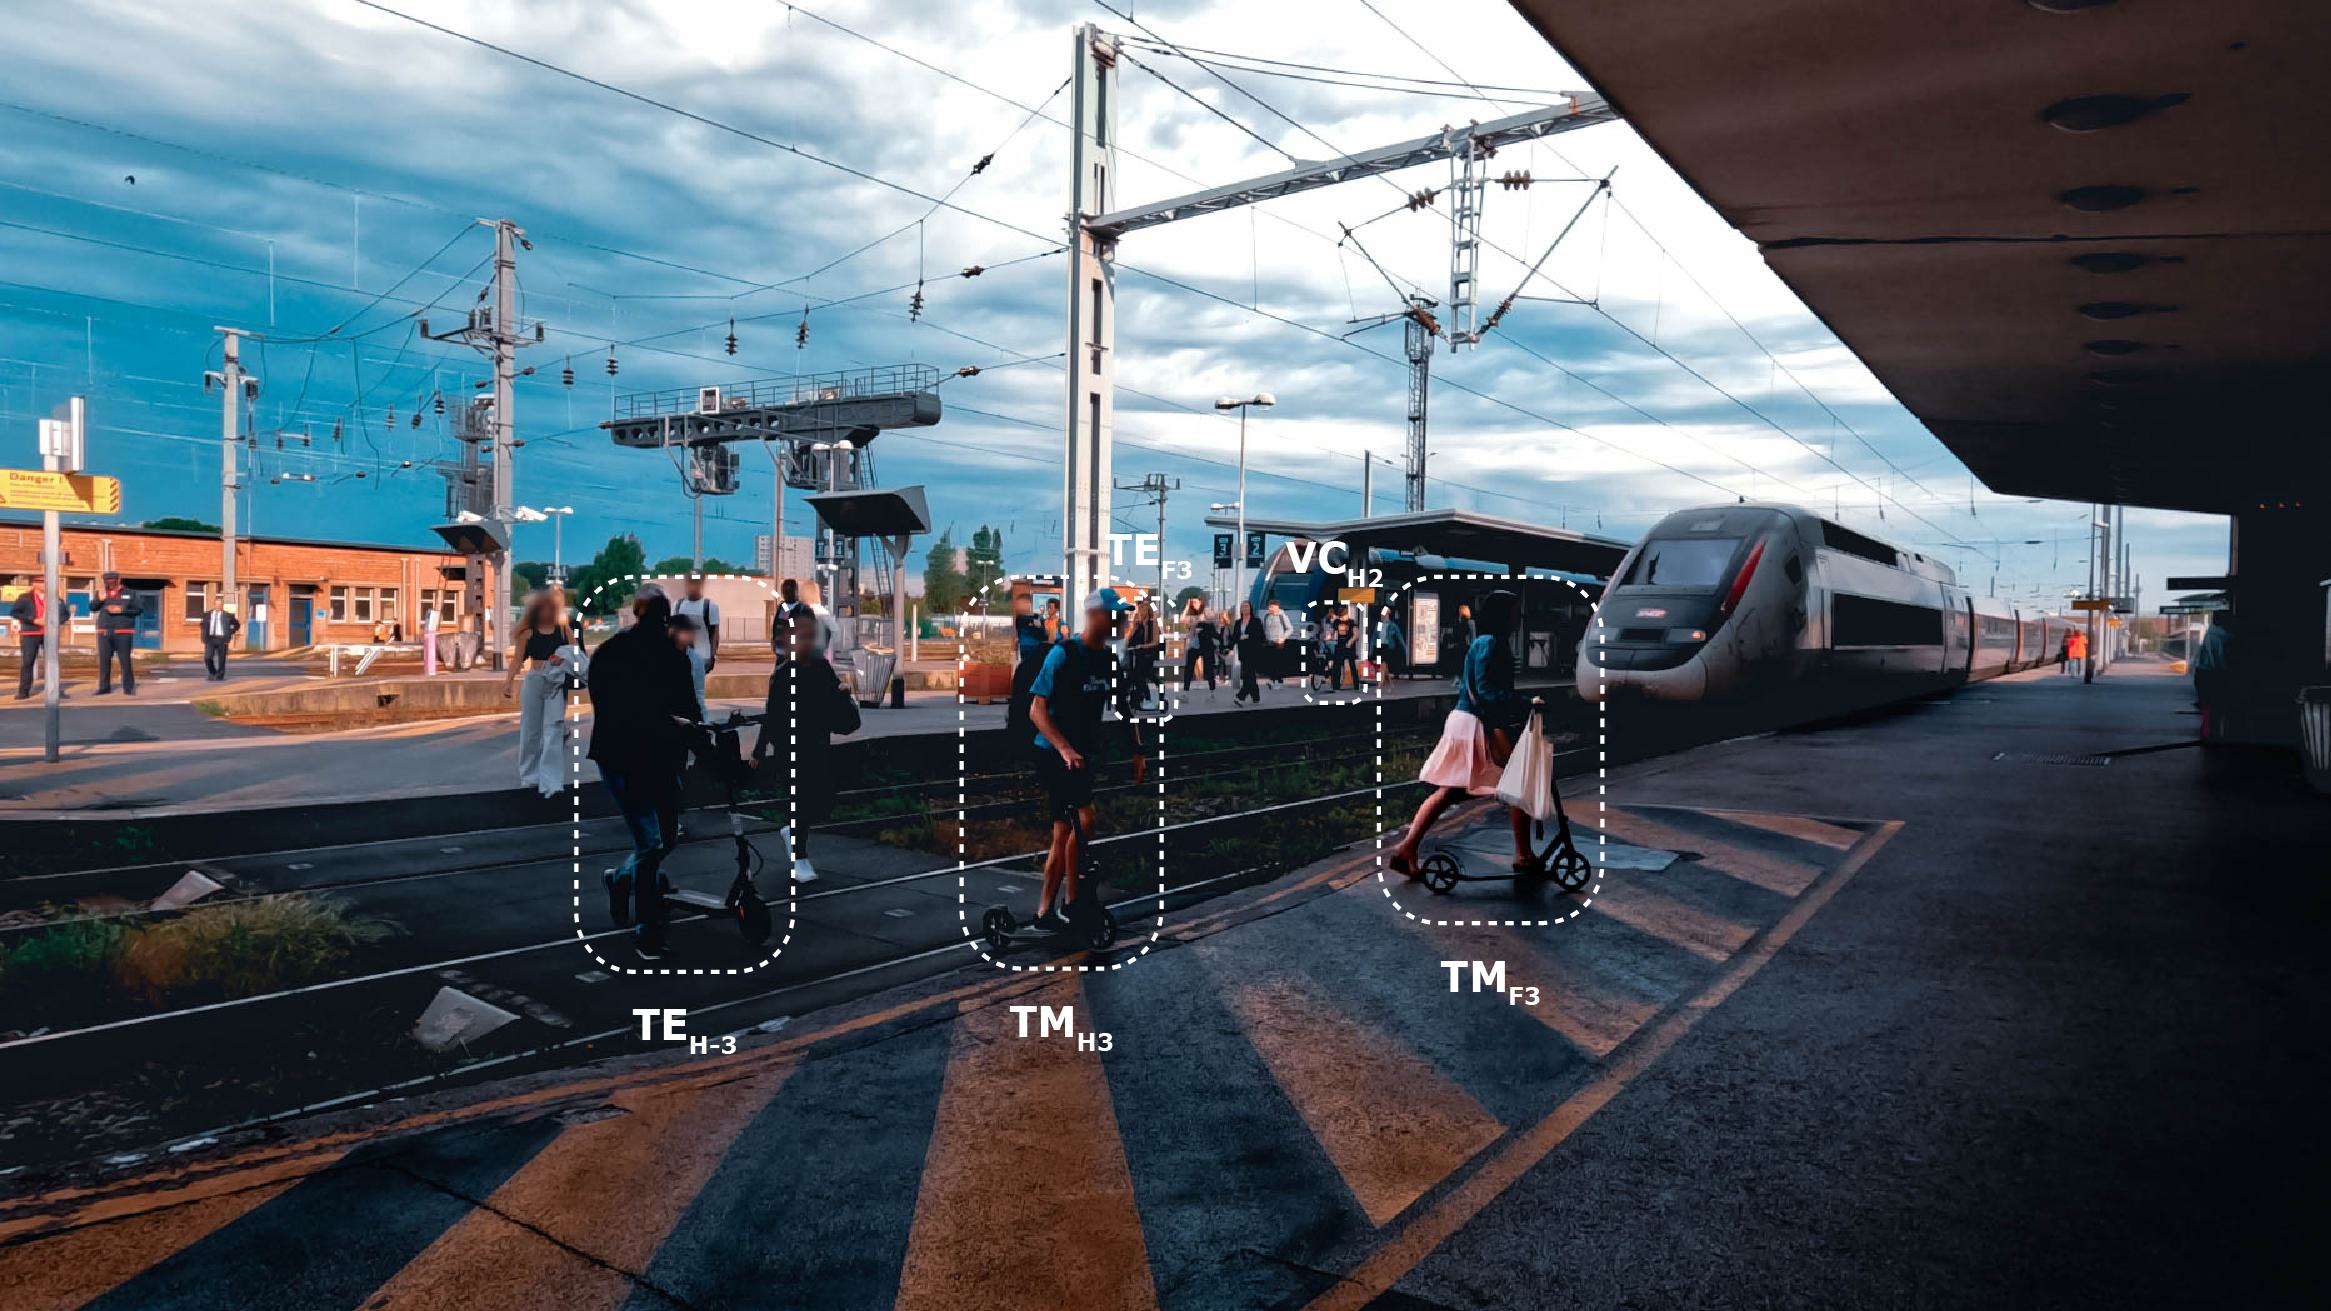
\includegraphics[width=1\columnwidth]{src/Figures/Chap-3/FR_Observation_Codes_Gare_Dunkerque.jpg}}
        \vspace{5pt}
        \begin{flushright}\scriptsize{
        Auteur~: \textcolor{blue}{Dylan Moinse (2022)}
        %\\
        %Réalisation avec la caméra \Marque{HERO10}~et sur \Marque{Photoshop}
        }\end{flushright}
    \end{figure}
    
    % Inspirations
En empruntant la technique de l’observation quantitative, notre recherche s'inspire de travaux antérieurs sur la répartition genrée de l'usage du vélo à partir d'observations sur le terrain \textcolor{blue}{\autocite[]{raibaud_femmes_2020}}\index{Raibaud, Yves|pagebf} et sur des déplacements impliquant l'utilisation conjointe du vélo et des transports en commun \textcolor{blue}{\autocites[192]{sherwin_practices_2011}[27]{la_paix_puello_modelling_2015}}\index{Sherwin, Henrietta|pagebf}\index{Parkhurst, Graham|pagebf}\index{Robbins, Derek|pagebf}\index{Walker, Ian|pagebf}\index{La Paix Puello, Lissy|pagebf}\index{Geurs, Karst~T.|pagebf}, tout en réinterprétant cette approche sous l'angle de l'intermodalité. L'\Guillemets{observiaire}~prenant la forme d'une caméra fixe et mis en place par \textcolor{blue}{\textcite[99]{cochoy_mort_2013}}\index{Cochoy, Franck|pagebf}\index{Calvignac, Cédric|pagebf} a grandement inspiré le choix de cette approche par observation directe, dans la mesure où ces dernier·ère·s ont pu faire valoir des résultats innovants en lien avec une \Guillemets{pratique ordinaire}~telle que la question de l'équipement des vélos \textcolor{blue}{\autocite[8]{cochoy_bicycles_2019}}\index{Cochoy, Franck|pagebf}\index{Hagberg, Johan|pagebf}\index{Normark, Daniel|pagebf}\index{Ducourant, Hélène|pagebf}\index{Holmberg, Ulrika|pagebf}\index{Calvignac, Cédric|pagebf}. C'est à ce titre que notre observation quantitative prend appui sur leur grille d'observation qui tente d'estimer diverses caractéristiques, tant socio-démographiques, physiques, techniques que socio-géographiques~: nous avons notamment repris certaines variables telles que le genre et l'âge et le type de vélo.%%Rédigé%%

    % Transition
La description de notre enquête par observation directe, ayant d'ores et déjà exposé l'échelle d'analyse objectale, qui concerne la catégorisation des variables examinées, s'apprête désormais à explorer les deux autres dimensions qui caractérisent l'observation quantitative. La section suivante se consacrera à détailler les modalités d'application de l'approche à partir de ses aspects spatiaux (découpage) et temporels (séquençage).%%Rédigé%%

    % 3.3.2.2.
    \needspace{1\baselineskip} % Réserve de l'espace
\subsubsection*{Mise en application de l'observation quantitative
    \label{chap3:application-observation-quantitative}
    }

    % Quais
Cette enquête par observation a été mise en œuvre sur les quais de gares ferroviaires préalablement sélectionnées. Cette démarche a pour objectif d'appréhender les flux de voyageur·se·s se dirigeant vers la gare (phénomène de rabattement) ainsi que ceux émanant de celle-ci (phénomène de diffusion). La décision de concentrer l'observation sur les quais est le résultat de la recherche d'un équilibre entre le respect des impératifs de sécurité en vigueur dans les gares, en minimisant l'impact de notre présence sur les flux de voyageur·se·s, tout en s'assurant de couvrir la totalité de ces flux. Cette approche s'est avérée d'autant plus pertinente au regard des conclusions d'un rapport d'étude produit par \textcolor{blue}{\textcite[13]{enov_enquete_2021}}\index{Enov@\textsl{Enov}|pagebf}, lequel indique que la grande majorité des cyclo-voyageur·se·s ont pour habitude d'embarquer leur véhicule à bord des trains. En conséquence, l'observation réalisée sur les quais s'est révélée être un moyen efficace pour capturer une proportion significative de voyageur·se·s intermodaux·les (voir le \hyperref[table-chap3:application-observation-quantitative-gares-examinees]{tableau~\ref{table-chap3:application-observation-quantitative-gares-examinees}}, page~\pageref{table-chap3:application-observation-quantitative-gares-examinees}).%%Rédigé%%

    % Tableau Gares étudiées
% Tableau Gares étudiées
%%Rédigé%%
  \begin{table}[h!]
    \centering
    \renewcommand{\arraystretch}{1.5}
    \resizebox{\columnwidth}{!}{
    \begin{tabular}{p{0.28\columnwidth}p{0.2\columnwidth}p{0.2\columnwidth}p{0.20\columnwidth}p{0.12\columnwidth}}
      % \hline
      \rule{0pt}{15pt} \small{\textcolor{blue}{\textbf{Gare ou halte}}} & \small{\textcolor{blue}{\textbf{Période (2022)}}} & \small{\textcolor{blue}{\textbf{Comptage*}}} & \small{\textcolor{blue}{\textbf{Trains}}} & \small{\textcolor{blue}{\textbf{Flux}}}\\
      \hline
    \multicolumn{5}{l}{\textbf{Gares de pôles régionaux}}\\
\small{Lille Flandres (\(G_1\))} & \small{5 et 7 avril} & \small{\textbf{5~836} (4,8~\%)} & \small{40 \acrshort{TGV} et \acrshort{TER}} & \small{21~992~946}\\
\small{Dunkerque (\(G_2\))} & \small{17 et 19 mai} & \small{\textbf{2~221} (21,2~\%)} & \small{28 \acrshort{TERGV} et \acrshort{TER}} & \small{1~905~250}\\
\small{Béthune (\(G_3\))} & \small{26 et 28 avril} & \small{\textbf{1~281} (14,6~\%)} & \small{13 \acrshort{TGV} et \acrshort{TER}} & \small{1~601~485}\\
\small{Armentières (\(G_4\))} & \small{3 et 5 mai} & \small{\textbf{2~324} (49,9~\%)} & \small{31 TER} & \small{850~773}\\
      \hdashline
\multicolumn{5}{l}{\textbf{Gare à rayonnement francilien}}\\
\small{Creil (\(G_5\))} & \small{7 et 9 juin} & \small{\textbf{2~159} (7,5~\%)} & \small{28 \acrshort{TER} et \acrshort{RER}} & \small{5~224~702}\\
      \hdashline
    \multicolumn{5}{l}{\textbf{Gares de rabattement sur les pôles régionaux}}\\
\small{Lille CHR (\(G_6\))} & \small{12 et 14 avril} & \small{\textbf{1~025} (59,9~\%)} & \small{42 \acrshort{TER}} & \small{312~323}\\
\small{Lesquin (\(G_7\))} & \small{19 et 21 avril} & \small{\textbf{309} (40,0~\%)} & \small{27 \acrshort{TER}} & \small{141~025}\\
\small{Le Poirier Université (\(G_8\))} & \small{10 et 12 mai} & \small{\textbf{280} (60,6~\%)} & \small{43 \acrshort{TER}} & \small{84~268}\\
\small{Vis-à-Marles (\(G_9\))} & \small{31 mai et 2 juin} & \small{\textbf{3} (3,2~\%)} & \small{2 \acrshort{TER}} & \small{17~063}\\
      \hdashline
    \multicolumn{5}{l}{\textbf{Échantillon complet}}\\
\multicolumn{2}{l}{\small{Neuf gares (18 jours, du 5 avril au 2 juin)}} & \small{\textbf{15~438} (8,5~\%)} & \small{254 trains} & \small{33~341~579}\\
      \hline
    \end{tabular}}
    \caption{Aperçu des neuf gares de la région Hauts-de-France formant le cadre géographique de l'observation quantitative.}
    \label{table-chap3:application-observation-quantitative-gares-examinees}
    \vspace{5pt}
        \begin{flushleft}\scriptsize
        \textcolor{blue}{Note~:} le comptage se réfère à l'échantillon récolté pour chacune des gares. Les proportions représentent quant à elles la part de voyageur·se·s observé·e·s par rapport à leur fréquentation quotidienne en 2022.
        \\
        \textcolor{blue}{Lecture~:} parmi les neuf gares ayant fait l'objet de séances d'observation quantitative au cours d'un mardi et d'un jeudi, nous avons pu capturer environ 8,5~\% des flux quotidiens.
        \end{flushleft}
        \begin{flushright}\scriptsize
        Jeux de données~: \textsl{SNCF Open Data} \textcolor{blue}{\autocite{sncf_frequentation_2024}}
        \\
        Auteur~: \textcolor{blue}{Dylan Moinse (2023)}
        \end{flushright}
        \end{table}%%Rédigé%%

    % Horaires et jours
Dans une enquête par observation, nous alternons des \Guillemets{séances d’observation} et des moments de réflexion et d’écriture sur ce qui a été observé qu'il convient de décrire \textcolor{blue}{\autocite[15]{revillard_observation_2018}}\index{Revillard, Anne|pagebf}. Dans le cadre de notre observation quantitative, les séances d'observation se sont déroulées les mardis et jeudis, sur une période de mars à mai 2022, en excluant les vacances pédagogiques, et ce, entre 07h00 et 10h00 puis entre 16h30 et 19h00. Ce cadrage temporel, appelé séquençage, a été défini dans le but de coïncider avec les pics d'affluence habituellement identifiés et qui correspondent principalement aux déplacements pendulaires, conformément aux recommandations de collecte des flux de cyclistes dans un territoire donné émises par \textcolor{blue}{\textcite[20]{johnstone_collecting_2017}}\index{Johnstone, Dylan|pagebf}\index{Nordback, Krista|pagebf}\index{Lowry, Michael~B.|pagebf}. Cette démarche s'appuie sur les conclusions de diverses études sur la fréquentation des \acrshort{TER}, mettant en évidence une prédominance de voyageur·se·s sur ces plages horaires. La temporalité générale des séances conduites se base également sur les travaux de \textcolor{blue}{\textcite[20]{johnstone_collecting_2017}}\index{Johnstone, Dylan|pagebf}\index{Nordback, Krista|pagebf}\index{Lowry, Michael~B.|pagebf}, qui préconisent alors de concentrer les séances d'observation auprès des cyclistes durant les périodes allant de mai à septembre, hors vacances scolaires et en semaine, en couvrant idéalement les tranches d'horaires s'étendant de 07h00 à 09h00, de 11h00 à 13h00 et de 16h00 à 18h00.%%Rédigé%%

    % Temporalité
Les séances d'observation se sont généralement déroulées durant une vingtaine de minutes chacune. Pour chaque \acrshort{TGV} ou \acrshort{TER} faisant l'objet de notre enquête, notre arrivée sur le quai s'effectuait une vingtaine de minutes avant son départ prévu, permettant ainsi de saisir l'ensemble des voyageur·se·s attendant ou montant dans le train (rabattement). Suite à l'arrivée du train, notre attention se portait sur les voyageur·se·s descendant du mode collectif (diffusion), jusqu'au départ de celui-ci en sens inverse et l'absence de tout usager·ère sur le quai. Cette technique d'observation justifie à nouveau le recours à la vidéographie, nécessitant un double visionnage de chaque séquence vidéo pour distinguer les flux entrants et sortants, les deux groupes de voyageur·se·s se côtoyant durant les périodes d'arrêt du train.%%Rédigé%%

    % ___________________________________________
    % Encadré exemple séance d'observation
    \begin{tcolorbox}[colback=white!5!white,
                      colframe=blue!75!blue, 
                      title=
                      \bigskip
                      \center{Illustration d'une séance d'observation quantitative}
                      \bigskip]
\normalsize{\textbf{Exemple du \acrshort{TER} reliant les gares de Lille Flandres, de Saint-Quentin et d'Amiens~:}}
    \\\\
\small{À titre d'illustration, notre première séance d'observation s'est déroulée en gare Lille Flandres, le mardi 5 avril 2022. Cette séquence s'est concentrée sur le même \acrshort{TER} arrivant à 07h07 et repartant pour 07h23 depuis la voie 2. Il s'agit alors d'un train qui suit la ligne K44 en provenance d'Amiens pour 05h50 et desservant principalement les gares d'Arras et de Douai. Et ensuite la ligne K40 en direction de la gare de Saint-Quentin en desservant principalement les gares de Douai et de Cambrai, pour une arrivée prévue à 09h14.}
    \\\\
\small{Après un entretien bref avec le chef de gare, nous avons procédé à l'installation du matériel à 06h50, en vue d'un enregistrement vidéographique débutant à 07h02. En raison de la complexité et de l'intensité des flux en gare Lille Flandres, le positionnement optimal de l'appareil d'enregistrement et de l'affichage a nécessité un temps supplémentaire imprévu afin de repérer un emplacement stratégique. À ce stade, la voie 2 étant encore vide, nous avons pu commencer à enregistrer les usager·ère·s se rendant sur le quai. À 07h09, le \acrshort{TER} ciblé arrive à quai, avec un retard de deux minutes. L'enregistrement se poursuit alors pour capter les voyageur·se·s de la ligne K44 débarquant de ce train. La séance s'achève à 07h27, après le départ du train de la ligne K40, et une fois le quai vidé de ses usager·ère·s.}
    \\\\
\small{Cette observation de 20 minutes a alors permis d'observer les pratiques de mobilité tant sur la ligne K44 en direction de Lille depuis Amiens (05h50 - 07h07) que sur la ligne K40 en direction de Saint-Quentin depuis Lille. Durant cette séance, diverses observations qualitatives ont été documentées dans notre journal de bord : un·e usager·ère circulant en \acrfull{TEP} et rappelé·e à l'ordre, le dénombrement de quatre voyageur·se·s à pied équipé·e·s de casques de vélo, un·e autre avec un casque de moto, ainsi qu'une tendance des voyageur·se·s accompagné·e·s d'un vélo classique à sortir en dernier du \acrshort{TER}, contrairement à celleux équipé·e·s d'un vélo pliant ou d'une \acrshort{TEP}. En conclusion de cette séance d'observation, une fiche dédiée a été remplie pour renseigner les conditions météorologiques, qualifiées de nuageuses avec une température de 12°C, et le retard de deux minutes observé à l'arrivée du train de la ligne K44.}
    \end{tcolorbox}

    % Météo et perturbations
En outre, la dimension temporelle de notre étude a été enrichie par une contextualisation des séances d'observation en fonction des conditions météorologiques et des aléas du système de transport. Chaque session a été systématiquement accompagnée d'informations relatives à la météo, celle-ci exerçant une influence notable sur l'usage de la mobilité individuelle légère, comme établi dans la \hyperref[chap2:impacts-meteo-saisons]{section dédiée aux effets des variations météorologiques} (page~\pageref{chap2:impacts-meteo-saisons}) dans le cadre du \hyperref[chap2:titre]{chapitre~2} (page~\pageref{chap2:titre}). Enfin, les perturbations affectant le réseau ferroviaire ont été renseignées lors de chaque séance d'observation, incluant la nature de la perturbation, le motif annoncé et la durée des retards éventuels.%%Rédigé%%

    % Figure caméra Lille Flandres
    \begin{figure}[h!]\vspace*{4pt}
        \caption{Déploiement de l'équipement sur les quais de la gare Lille Flandres désignée pour l'observation quantitative, le 5 avril 2022.}
        \label{fig-chap3:materiel-observation-quantitative}
        \centerline{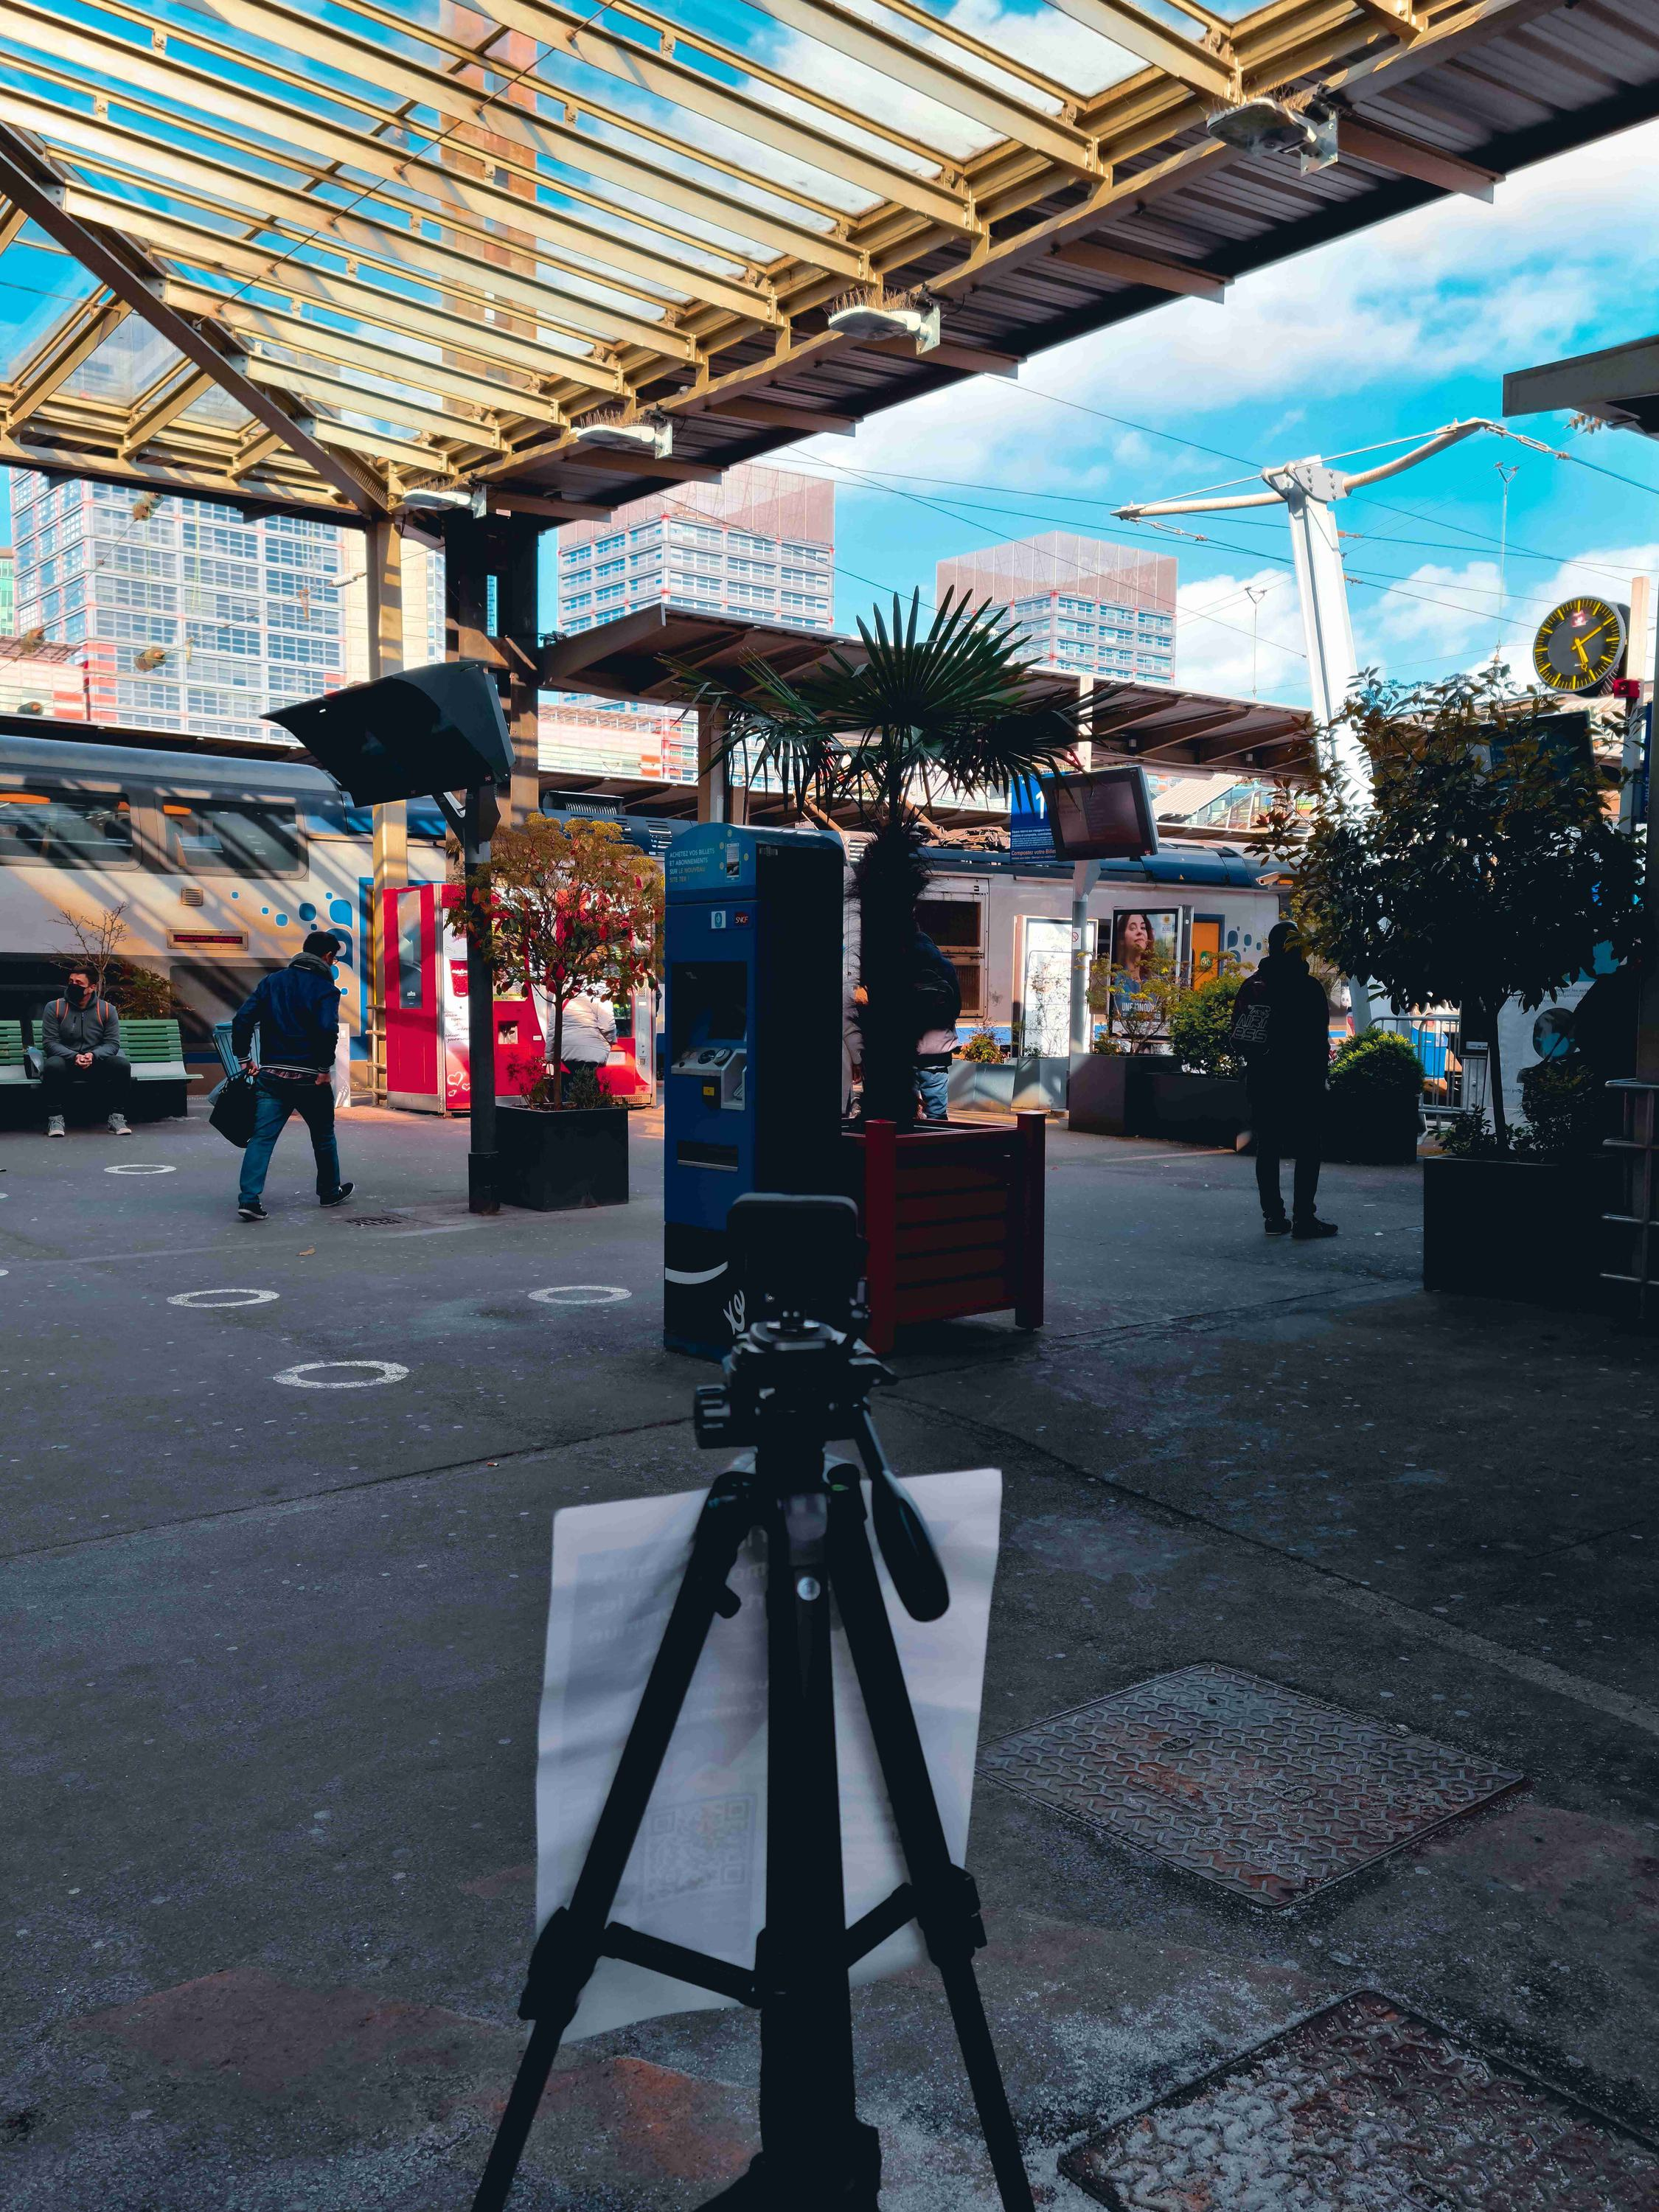
\includegraphics[width=0.5\columnwidth]{src/Figures/Chap-3/FR_Observation_Camera_Lille_Flandres.jpg}}
        \vspace{5pt}
        \begin{flushright}\scriptsize{
        Auteur~: \textcolor{blue}{Dylan Moinse (2022)}
        }\end{flushright}
    \end{figure}

    % Matériel
Dans le cadre de notre collaboration avec \textsl{SNCF Gares \& Connexions}, nous avons alors suivi un protocole méthodologique précisément défini. L'équipement choisi pour cette méthode d'enquête est la caméra d'action \textsl{HERO10} de la marque \Marque{GoPro}\footnote{
Cet instrument portable, monté sur un trépied, se prête idéalement à l'immersion dans l'environnement des quais de gare, fournissant des enregistrements d'une qualité ultra haute définition avec une résolution de 4K.}, disposée sur les quais des gares (voir l'\hyperref[fig-chap3:materiel-observation-quantitative]{illustration~\ref{fig-chap3:materiel-observation-quantitative}}, page~\pageref{fig-chap3:materiel-observation-quantitative}). La mise en œuvre de cette méthode s'est systématiquement effectuée sous la supervision de deux intervenant·e·s, dont le responsable du projet, vêtu·e·s d'un gilet officiel \Guillemets{SNCF Gares \& Connexions}\footnote{
L'adoption d'un gilet distinctif, à l'initiative du gestionnaire des gares, a contribué à accroître notre crédibilité auprès de voyageur·se·s légitimement intrigué·e·s par notre présence et par le matériel mobilisé. Toutefois, cette même tenue a également été à l'origine de quelques situations imprévues, voire de moments d'inconfort. En effet, certain·e·s usager·ère·s s'attendaient à interagir avec le personnel compétent. Cette confusion a particulièrement été ressentie durant les périodes de perturbation du réseau ferroviaire, nous exposant à des situations potentiellement délicates. Notons que, si le port de ce gilet s'est avéré obligatoire dans certaines gares, il a été dans d'autres cas explicitement refusé par les responsables de gare. Ces dernier·ère·s ont préféré imposer le gilet orange, norme réglementaire sur les sites en travaux.
}. Conformément aux exigences du \acrshort{RGPD}, telles qu'énoncées dans les documents transmis aux \acrshort{DPO}, notre démarche a été accompagnée de l'installation d'un panneau d'information, visible à l'entrée et à la sortie des quais. Cette affiche apporte notamment aux voyageur·se·s les informations suivantes~:
    \begin{customitemize}
\item L'objectif de l'enquête~;
\item Le caractère exclusivement scientifique de la démarche~;
\item L'utilisation de techniques vidéographiques et la possibilité pour les individus de ne pas être filmés en se positionnant derrière la caméra, stratégiquement placée au centre du quai~;
\item Les coordonnées du responsable de traitement des données~;
\item La durée de conservation des données, prévue jusqu'en 2026~;
\item La base juridique du traitement des données et le droit d'introduire une réclamation à la \acrshort{CNIL}.
    \end{customitemize}%%Rédigé%%

    % Transition
Notre propos se poursuit par une présentation générale des neuf gares ayant servi de cadre spatial à nos séances d'observation quantitative.%%Rédigé%%

    % 3.3.3.
    \needspace{1\baselineskip} % Réserve de l'espace
\subsection{Choix des gares pour les séances d'observation
    \label{chap3:observation-quantitative-gares-examinees}
    }

    % Introduction
La sélection des gares de la région Hauts-de-France ayant fait l’objet d’une enquête par observation quantitative se fonde sur des considérations territoriales eu égard au potentiel de développement de la mobilité individuelle légère en articulation avec le système ferroviaire. En accord avec les recommandations de \textsl{SNCF Gares \& Connexions} s’agissant du nombre de gares interrogées, nous avons choisi d’étudier au total neuf gares qui nous semblent refléter certaines dynamiques représentatives de la région analysée.%%Rédigé%%

    % Carte de situation gares examinées
    \begin{carte}[h!]%\vspace*{4pt}
        \caption{Carte de situation de la région Hauts-de-France et des neuf gares examinées.}
        \label{fig-chap3:gares-examinees}
        \centerline{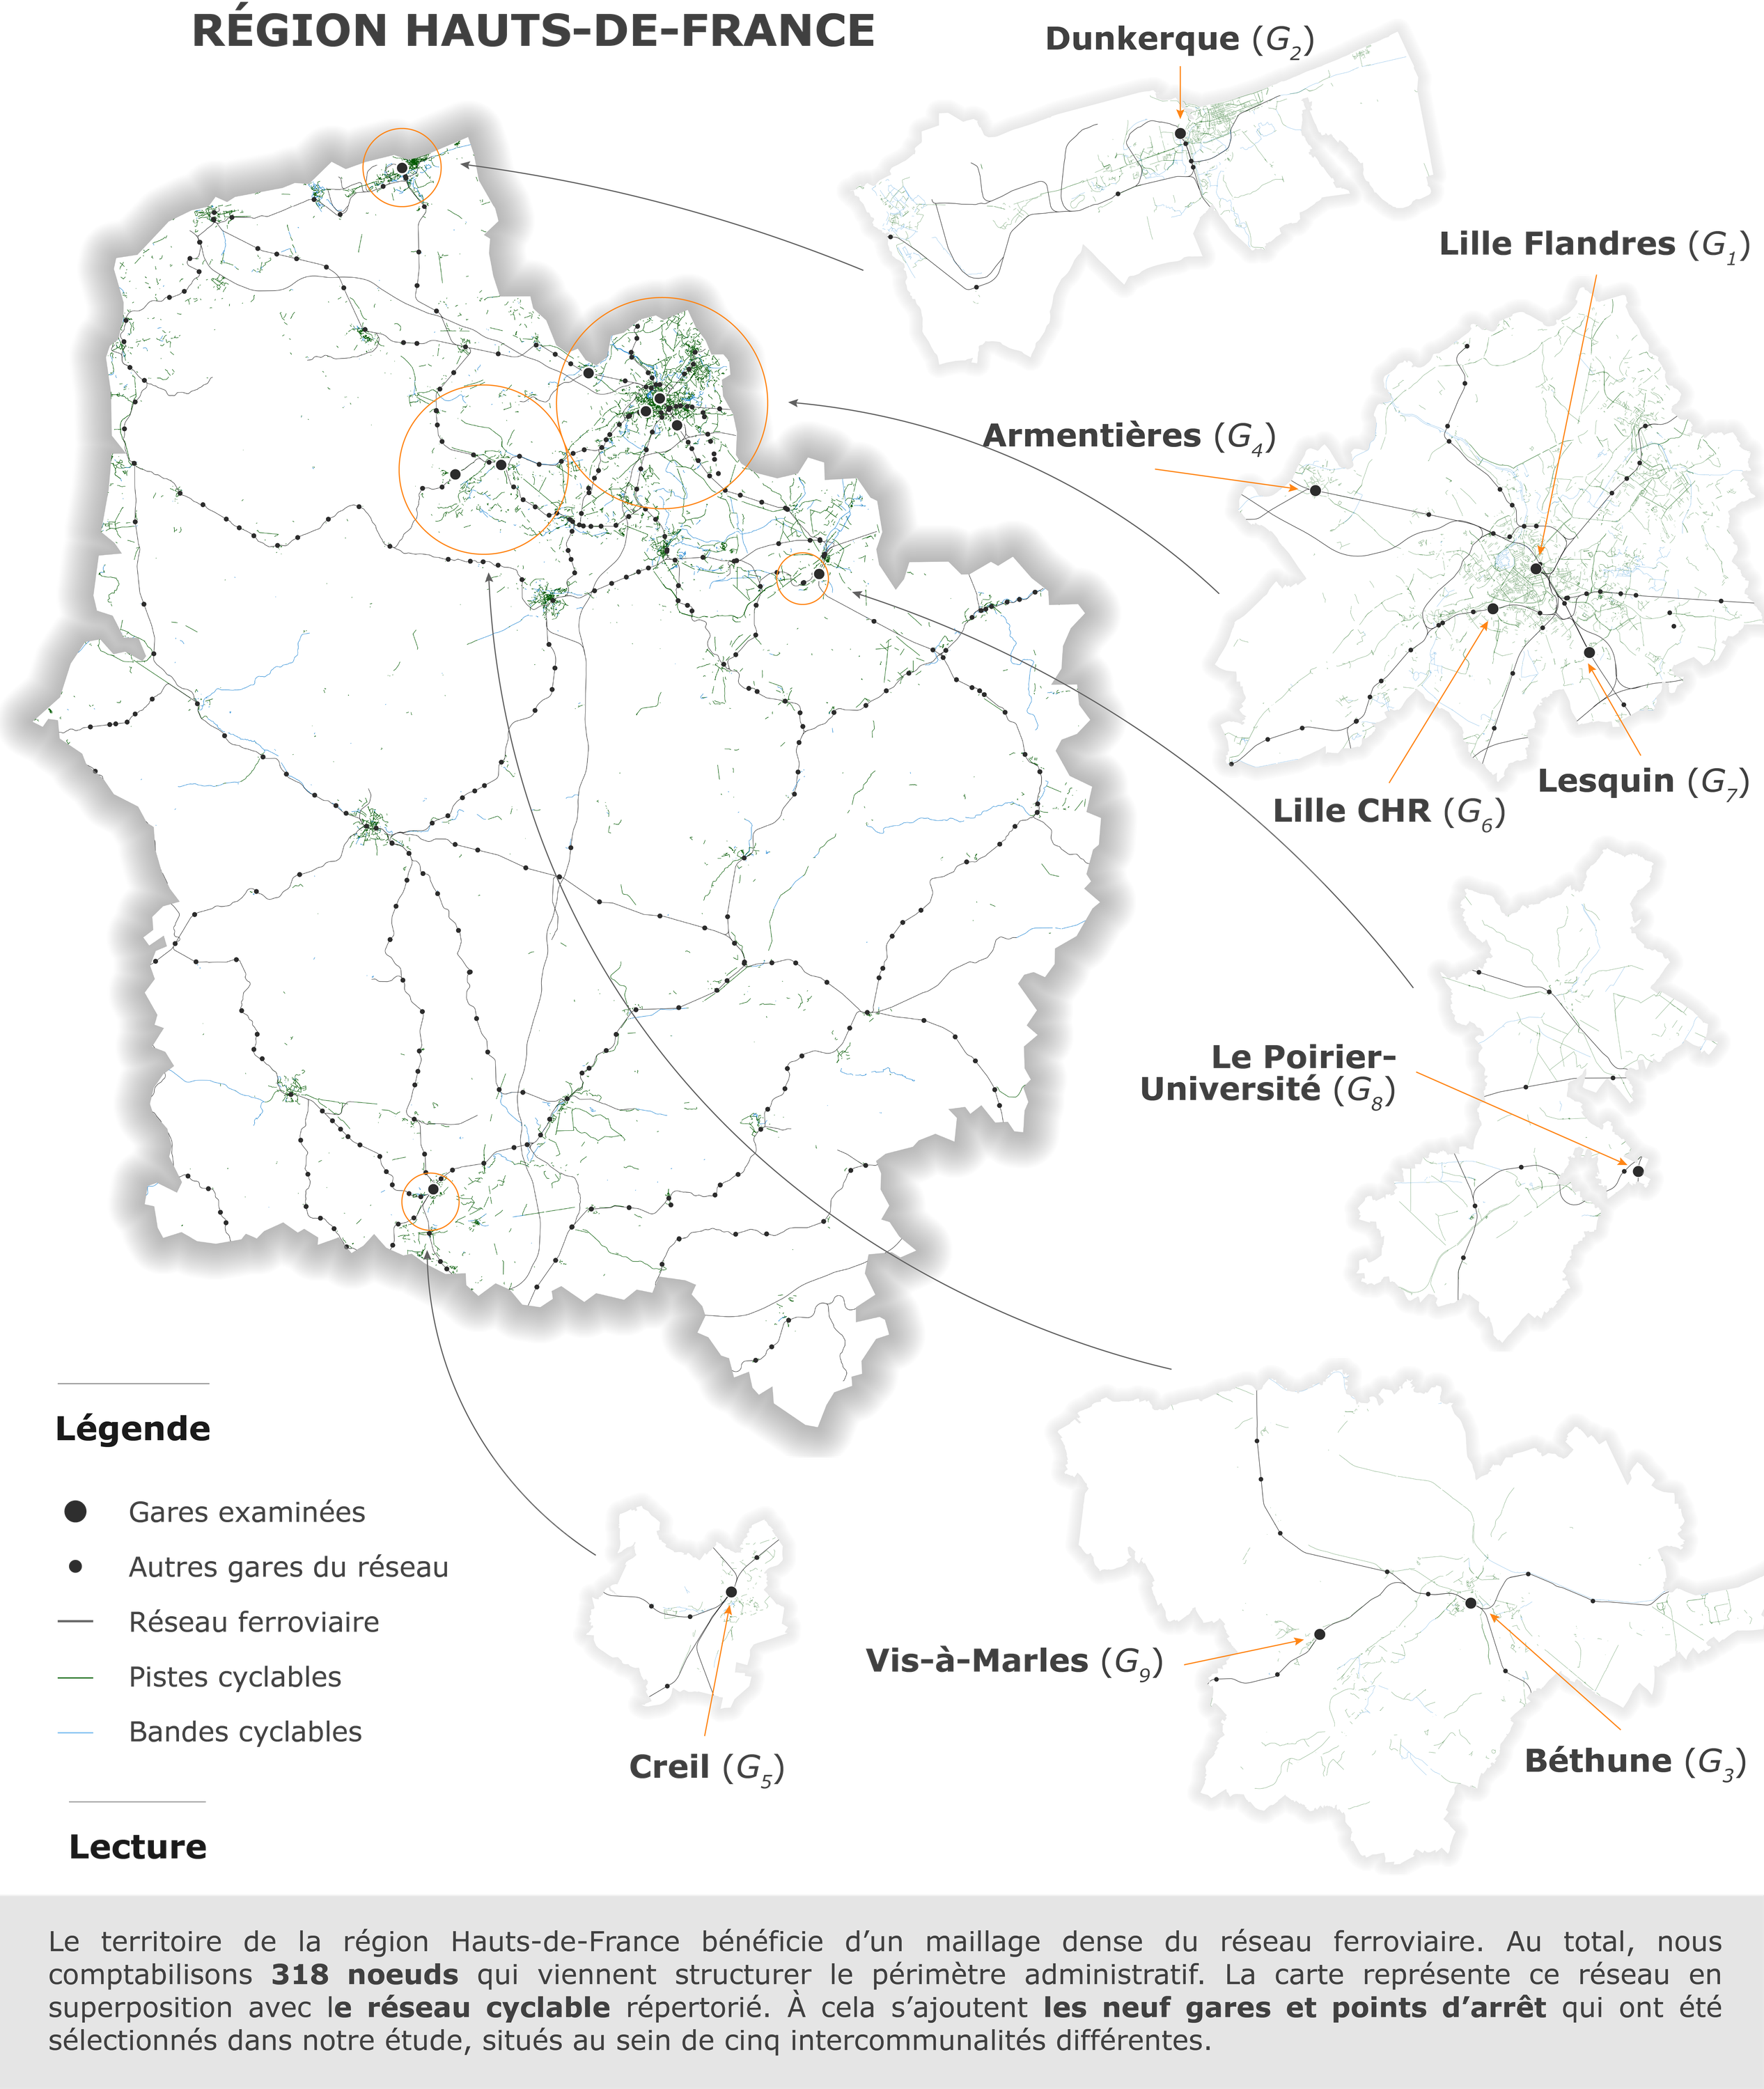
\includegraphics[width=1\columnwidth]{src/Figures/Chap-3/FR_Carte_situation_gares_examinees.png}}
        \vspace{5pt}
        \begin{flushright}\scriptsize{
        Jeux de données~: \textcolor{blue}{\textcite{openstreetmap_openstreetmap_2023}} et \acrshort{GTFS} de la \textcolor{blue}{\textcite{sncf_reseau_2024}}\index{SNCF@\textsl{SNCF}|pagebf}
        \\
        Auteur~: \textcolor{blue}{Dylan Moinse (2024)}
        }\end{flushright}
    \end{carte}

    % Gares examinées
La sélection des neuf gares étudiées au sein de la région Hauts-de-France repose sur une approche prenant en considération les enjeux territoriaux spécifiques liés au potentiel de développement de la mobilité individuelle légère dans leur environnement immédiat. Ce choix s’appuie sur la classification des gares de l’ancienne région Picardie \textcolor{blue}{\autocite[2-4]{cete_nord_picardie_profils_2011}}\index{CETE@\textsl{CETE}|pagebf}\index{DREAL@\textsl{DREAL}|pagebf}, ce qui a permis d’enrichir notre analyse territoriale. Notre première approche mobilise neuf terrains d’étude répartis comme suit~: les gares de Lille Flandres (\(G_1\)), Dunkerque (\(G_2\)), Béthune (\(G_3\)) et Armentières (\(G_4\)), identifiées comme des \Guillemets{gares de pôles régionaux}~; la gare de Creil (\(G_5\)), classée comme une \Guillemets{gare à rayonnement francilien}~; et enfin, les haltes de Lille CHR (\(G_6\)), Lesquin (\(G_7\)), Le Poirier Université (\(G_8\)) et Vis-à-Marles (\(G_9\)), considérées comme des \Guillemets{gares de rabattement sur les pôles régionaux} (voir la \hyperref[fig-chap3:gares-examinees]{carte~\ref{fig-chap3:gares-examinees}}, page~\pageref{fig-chap3:gares-examinees}).%%Rédigé%%

    % 3.3.3.1.
    \needspace{1\baselineskip} % Réserve de l'espace
\subsubsection*{Gare Lille Flandres~: d'un espace nodal central à un pôle multimodal et international
    \label{chap3:application-observation-quantitative-lille-flandres}
    }

    % Carte Lille Flandres (G1)
        \begin{carte}[h!]\vspace*{4pt}
        \caption{Monographie de la gare Lille Flandres.}
        \label{fig-chap3:monographie-lille-flandres}
        \centerline{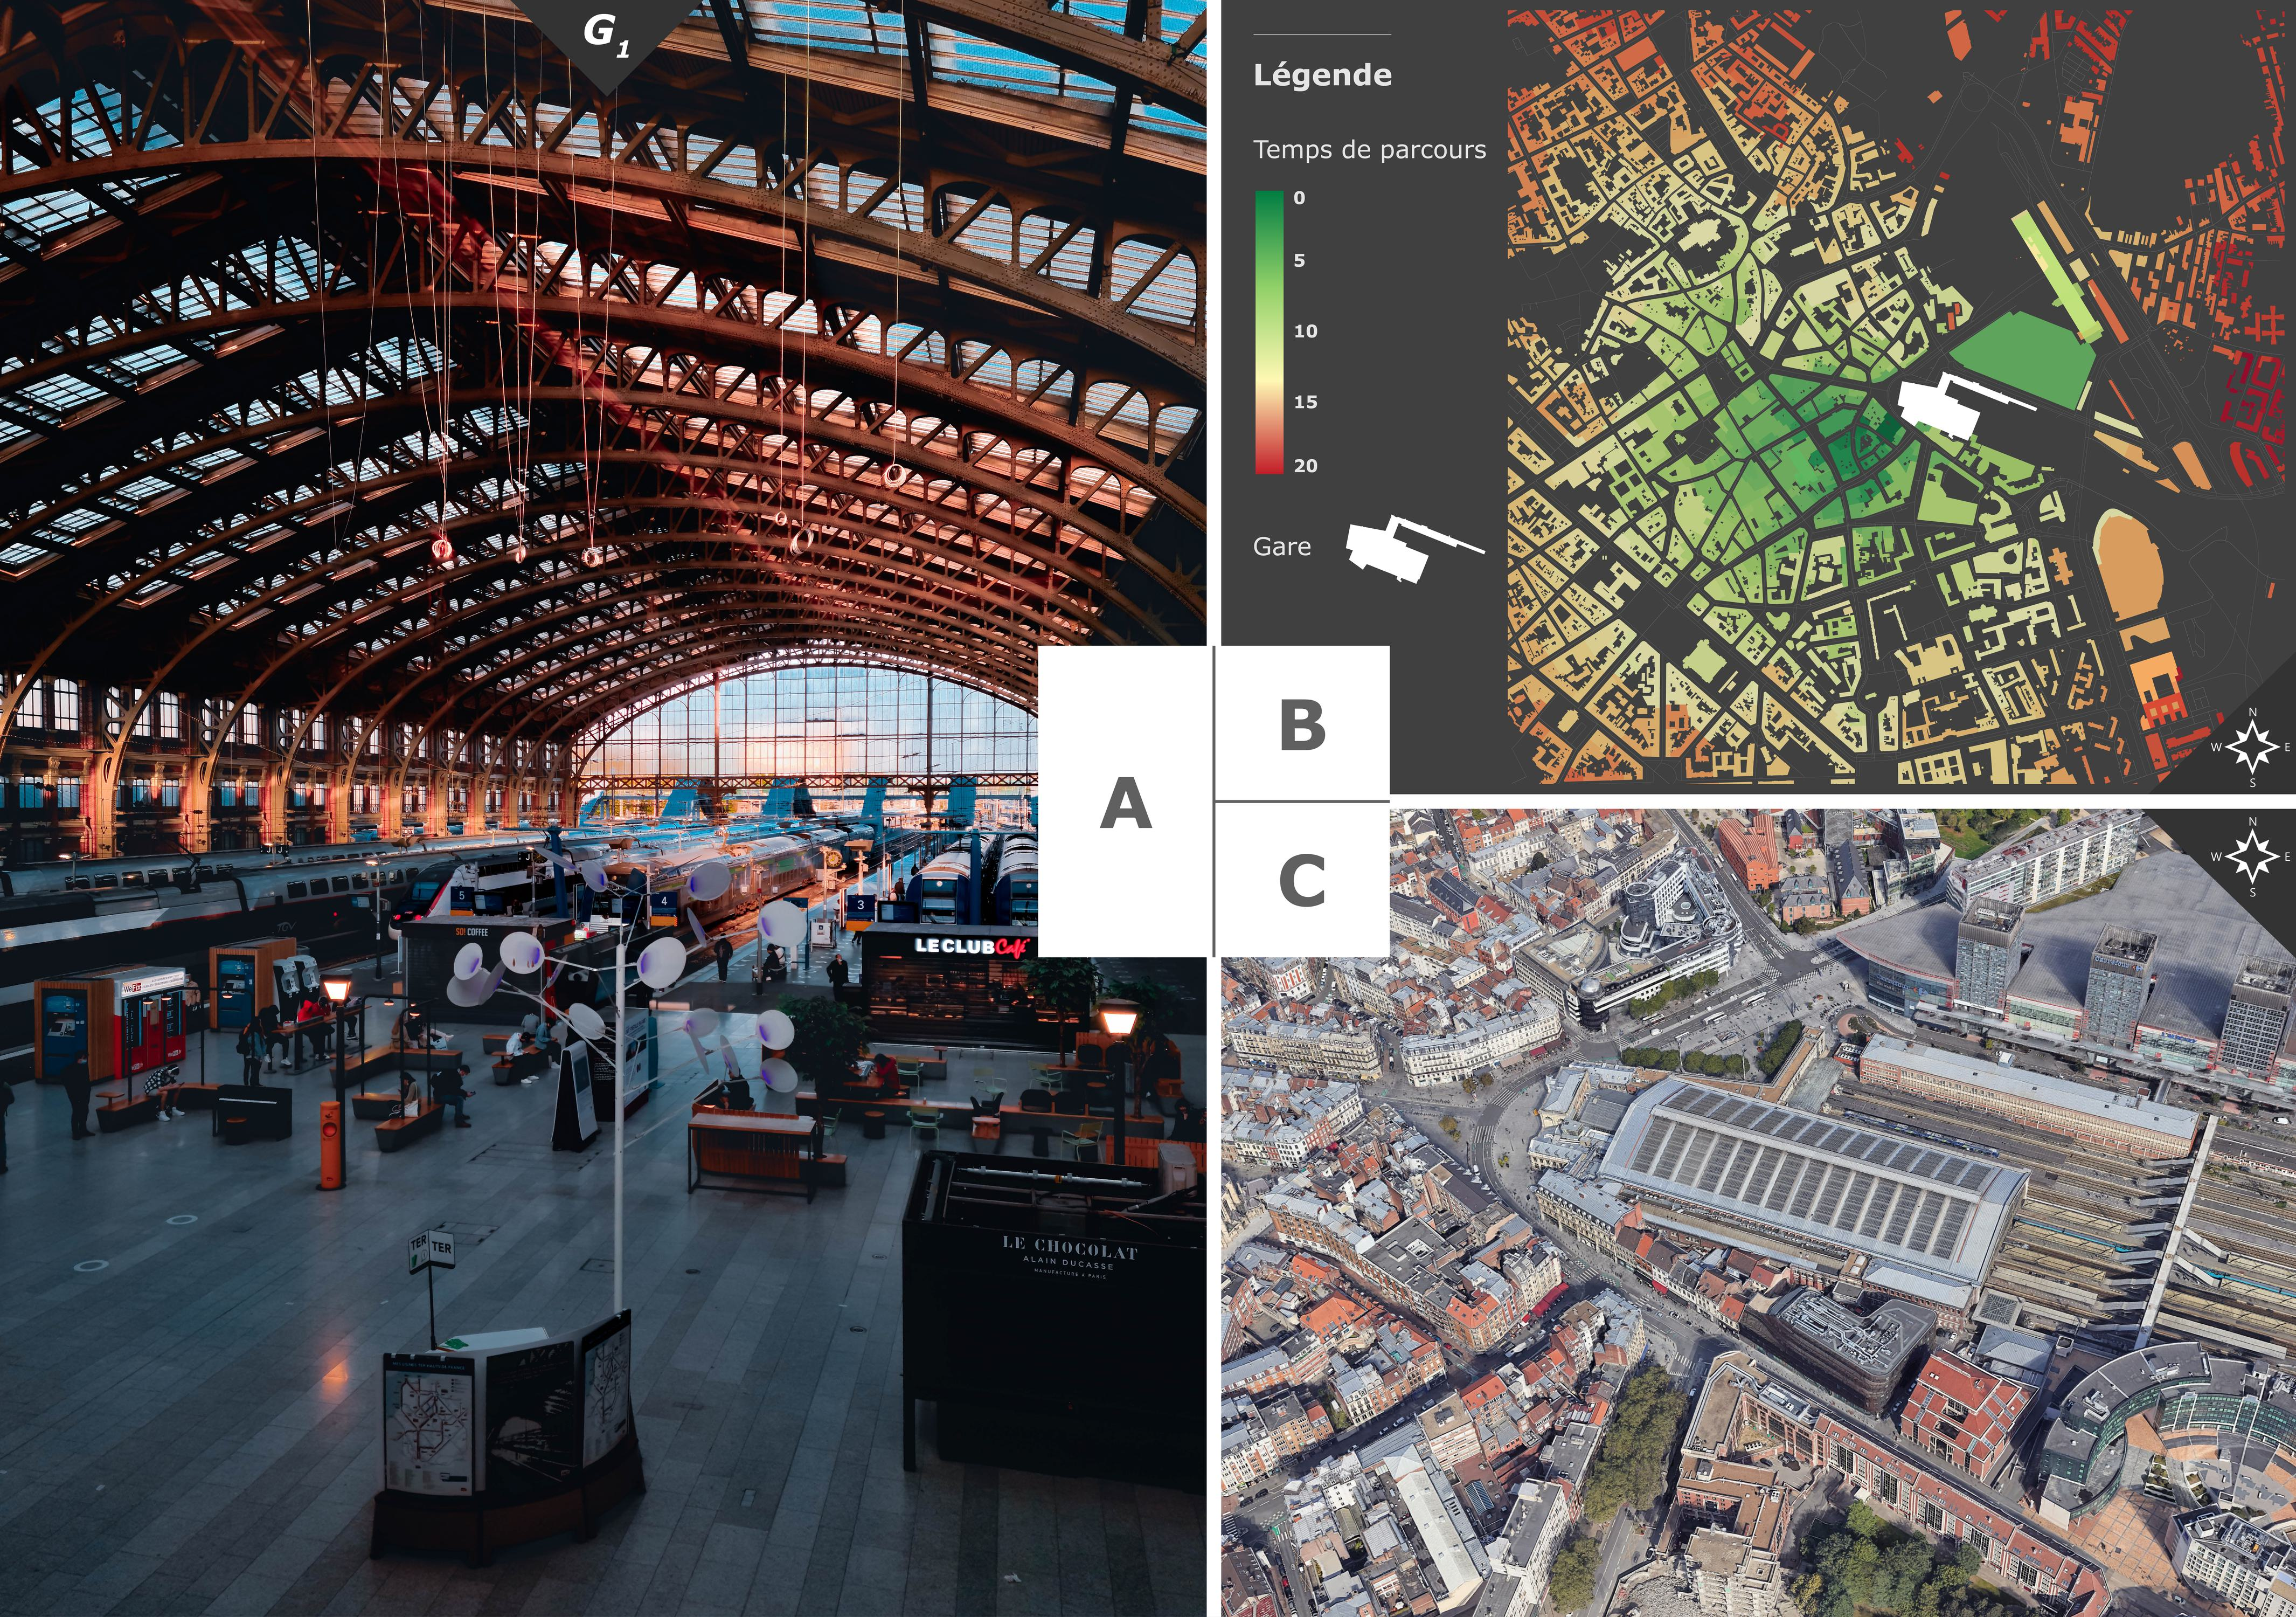
\includegraphics[height=.35\pageheight]{src/Figures/Chap-3/FR_Gare_Lille_Flandres}}
        \vspace{5pt}
        \begin{flushright}\scriptsize{
        Photographie (A)~: \textcolor{blue}{Dylan Moinse (2022)}
        \\
        Auteur (B)~: \textcolor{blue}{Dylan Moinse (2024)} avec les données issues d'\textcolor{blue}{\textcite{openstreetmap_openstreetmap_2023}}
        \\
      Jeux de données (C)~: données satellitaires issues de \textcolor{blue}{\textcite{google_earth_google_2023}}
      }\end{flushright}
      \end{carte}

    % Gare Lille Flandres (G1) (partie 1)
La gare Lille Flandres (\(G_1\)) concentre une part majeure du trafic ferroviaire régional\footnote{
    Avec un flux total de 24~118~203 voyageur·se·s en 2023, elle figure parmi les gares françaises les plus fréquentées, occupant la 15\textsuperscript{e} position au niveau national, et se hisse à la 2\textsuperscript{e} place hors Île-de-France, derrière Lyon Part-Dieu, selon les données du registre de fréquentation en gare publiées par la \textcolor{blue}{\textcite{sncf_frequentation_2024}}.
}, notamment lié aux navettes professionnelles à destination ou en connexion avec la capitale régionale \textcolor{blue}{\autocite[12]{hasiak_estimation_2018}}\index{Hasiak, Fabrice|pagebf}\index{Verdier, Laurent|pagebf}. La gare Lille Flandres est structurée en étoile ferroviaire, avec une configuration en cul-de-sac, et accueille des réseaux \acrshort{TER} et \acrshort{TGV}, principalement en provenance de Paris (voir la \hyperref[fig-chap3:monographie-lille-flandres]{carte~\ref{fig-chap3:monographie-lille-flandres}}, page~\pageref{fig-chap3:monographie-lille-flandres}). En nous référant à la typologie des pôles d'échange multimodaux établie dans le \acrshort{SRADDET} de la \textcolor{blue}{\textcite[81]{region_hauts-de-france_sraddet_2024}}\index{Région Hauts-de-France@\textsl{Région Hauts-de-France}|pagebf}, il s'agit d'un \Guillemets{pôle d'échange multimodal régional}. Elle est également desservie par deux lignes de métro, deux lignes de tramway, ainsi qu'un réseau dense de \acrshort{BHNS}\footnote{
    La configuration en cul-de-sac de la gare patrimoniale Lille Flandres est néanmoins appelée à évoluer. En effet, dans le cadre du projet de \acrfull{SERM} lillois, une nouvelle annexe souterraine est prévue entre les gares Lille Flandres et Lille Europe, permettant ainsi des traversées diamétrales par la capitale des Flandres \textcolor{blue}{\textcite{metropole_europeenne_de_lille_construisons_nodate}}. Parallèlement, le \acrfull{SDIT}, approuvé en 2019, prévoit la création d'une nouvelle ligne de tramway qui viendra directement desservir les deux gares lilloises, renforçant ainsi leur rôle stratégique au sein du réseau de mobilité métropolitain \textcolor{blue}{\textcite{metropole_europeenne_de_lille_service_2023}}.
}. De plus, la dynamique cyclable observée dans l’hypercentre lillois complète ce tableau~: le vélo qui tend à se démocratiser dans l'hypercentre bénéficie d’une infrastructure cyclable représentant 3,5~\% du réseau viaire, contre 2,5~\% à l’échelle nationale \textcolor{blue}{\autocite[103]{cordier_parts_2021}}\index{Cordier, Bruno|pagebf}. À l’échelle de la gare, la place accordée à la mobilité individuelle légère se manifeste notamment par l’inauguration, en 2019, d’une vélostation offrant plus de 500 places. Cet équipement est spécifiquement destiné aux abonné·e·s de la \textsl{SNCF} et du réseau \textsl{Ilévia} \textcolor{blue}{\autocite[]{adav_velostation_nodate}}\index{ADAV@\textsl{ADAV}|pagebf}.%%Rédigé%%

    % Figure Euraflandres avant-après
    \begin{figure}[h!]\vspace*{4pt}
        \caption{Vues aériennes du quartier d'\textsl{Euraflandres} réaménagé entre 2017 et 2019.}
        \label{fig-chap3:euraflandres-avant-apres}
        \centerline{\includegraphics[width=1\columnwidth]{src/Figures/Chap-3/FR_Euraflandres_avant_apres.png}}
        \vspace{5pt}
        \begin{flushright}\scriptsize{
        Jeux de données~: données satellitaires issues de \textcolor{blue}{\textcite{ign_remonter_2025}}\index{IGN@\textsl{IGN}|pagebf}
        }\end{flushright}
    \end{figure}

    % Gare Lille Flandres (G1) (partie 2)
Sa situation stratégique est renforcée par la proximité immédiate de la gare Lille Europe, située à moins de 500 mètres à pied, formant ainsi un véritable \Guillemets{orchestre des gares}\footnote{
    La distance à vol d'oiseau entre les deux gares est de 501 mètres, d'après la plate-forme \textsl{Géoportail} (\url{https://www.geoportail.gouv.fr/}) de l'\acrfull{IGN}. \textcolor{blue}{Nils} \textcolor{blue}{\textcite[415-416]{le_bot_quel_2019}}\index{Le Bot, Nils|pagebf} considère que les gares Lille Flandres et Lille Europe fonctionnent ainsi de concert, en étant finalement séparées (ou reliées) au centre commercial Euralille. Il s'agit d'un exemple remarquable de coopération gare-gare, cette configuration pouvant être qualifiée de \Guillemets{pôle Flandres}, qui incarne l'évolution \Guillemets{ultime} de la variable d'expansion des gares métropolitaines, au-delà de la seule échelle des bâtiments voyageur·se·s. L'expression \Guillemets{orchestre de gares} décrit alors un espace nodal où plusieurs gares, de par leur proximité géographique et la complémentarité de leurs offres, fonctionnent de manière coopérative, parfois au point de former un véritable \Guillemets{quartier-gare}, comme illustré par les deux gares lilloises.
} \textcolor{blue}{\autocite[415-416]{le_bot_quel_2019}}\index{Le Bot, Nils|pagebf}. Cette configuration aux \Guillemets{allures internationales} \textcolor{blue}{\autocite[334]{bertolini_nodes_1996}}\index{Bertolini, Luca|pagebf}, abordée dans la thèse de \textcolor{blue}{Nils} \textcolor{blue}{\textcite[415-416]{le_bot_quel_2019}}\index{Le Bot, Nils|pagebf} sous l'angle d'un \Guillemets{tandem} de gares métropolitaines, s'inscrit dans un projet urbain plus large, comprenant la piétonisation de la place des Buisses et la valorisation de la place François Mitterrand, aujourd'hui regroupées sous l'appellation \textsl{Euraflandres} (voir l'\hyperref[fig-chap3:euraflandres-avant-apres]{illustration~\ref{fig-chap3:euraflandres-avant-apres}}, page~\pageref{fig-chap3:euraflandres-avant-apres}). Ces requalifications urbaines se référant au programme \textsl{Euralille 3000} et porté par la \acrfull{SPL} Euralille\footnote{
    La \acrshort{SPL} Euralille occupe un rôle central dans la coordination et le développement du quartier d’affaires (\acrshort{CBD}) Euralille. Depuis les premières esquisses du projet d’aménagement en 1991, la \acrshort{SPL} a supervisé les différentes phases de développement \textcolor{blue}{\autocite[]{hayer_fabriquer_2005}}\index{Hayer, Dominique|pagebf}, à savoir~: \textsl{Euralille~I}, comprenant les secteurs \Guillemets{Central}, \Guillemets{Saint-Maurice} et \Guillemets{Chaude Rivière})~; \textsl{Euralille II}~; et plus récemment \textsl{Euralille III}, intégrant notamment la \acrfull{ZAC} \Guillemets{Porte de Valenciennes}. L’introduction de l’appellation \textsl{Euraflandres} apparaît pour la première fois dans le cadre du \acrshort{SCoT}, élaboré par la \acrfull{MEL} et mis en vigueur en 2017. Cette dénomination vise à caractériser les liens fonctionnels et spatiaux entre les pôles d’échange des gares Lille Flandres et Lille Europe et le quartier d’affaires Euralille \textcolor{blue}{\autocite[71]{adulm_rapport_2017}}.
}, vise à renforcer la connexion entre les pôles d'échange de Lille Flandres et Lille Europe et le quartier d'affaires Euralille \textcolor{blue}{\autocite[71]{adulm_rapport_2017}}\index{ADULM@\textsl{ADULM}|pagebf}. Cet ensemble incarne l’ambition de la métropole de se positionner comme une Eurocité, puis une Eurométropole, grâce à son intégration dans le schéma de desserte du \acrshort{TGV} nord-européen \textcolor{blue}{\autocite[155]{baron_reseaux_2017}}\index{Baron, Nacima|pagebf}\index{Messulam, Pierre|pagebf}, renforçant le processus de métropolisation et l'attractivité économique de la capitale régionale, sans que cela ait toutefois d'\Guillemets{effets structurants} automatiques \textcolor{blue}{\autocite[238]{offner__1993}}\index{Offner, Jean-Marc|pagebf} dans les territoires voisins \textcolor{blue}{\autocite[109]{chen_wider_2012}}\index{Chen, Chia-Lin|pagebf}\index{Hall, Peter|pagebf}. Cette configuration territoriale \Guillemets{hybride} constitue une vitrine de l'agglomération et de la région \textcolor{blue}{\autocite[2]{heddebaut_city-hubs_2018}}\index{Heddebaut, Odile|pagebf}\index{Di Ciommo, Floridea|pagebf}, conférant à cette transformation urbaine la qualité d'un quartier \acrshort{TOD}, selon \textcolor{blue}{\textcite[5]{heddebaut_city-hubs_2018}}\index{Heddebaut, Odile|pagebf}\index{Di Ciommo, Floridea|pagebf}.%%Rédigé%%

    % 3.3.3.2.
    \needspace{1\baselineskip} % Réserve de l'espace
\subsubsection*{Gares de Dunkerque et de Béthune~: pôles d'échange régionaux structurants
    \label{chap3:application-observation-quantitative-dunkerque-bethune}
    }

    % Carte Dunkerque (G2)
        \begin{carte}[h!]\vspace*{4pt}
        \caption{Monographie de la gare de Dunkerque.}
        \label{fig-chap3:monographie-dunkerque}
        \centerline{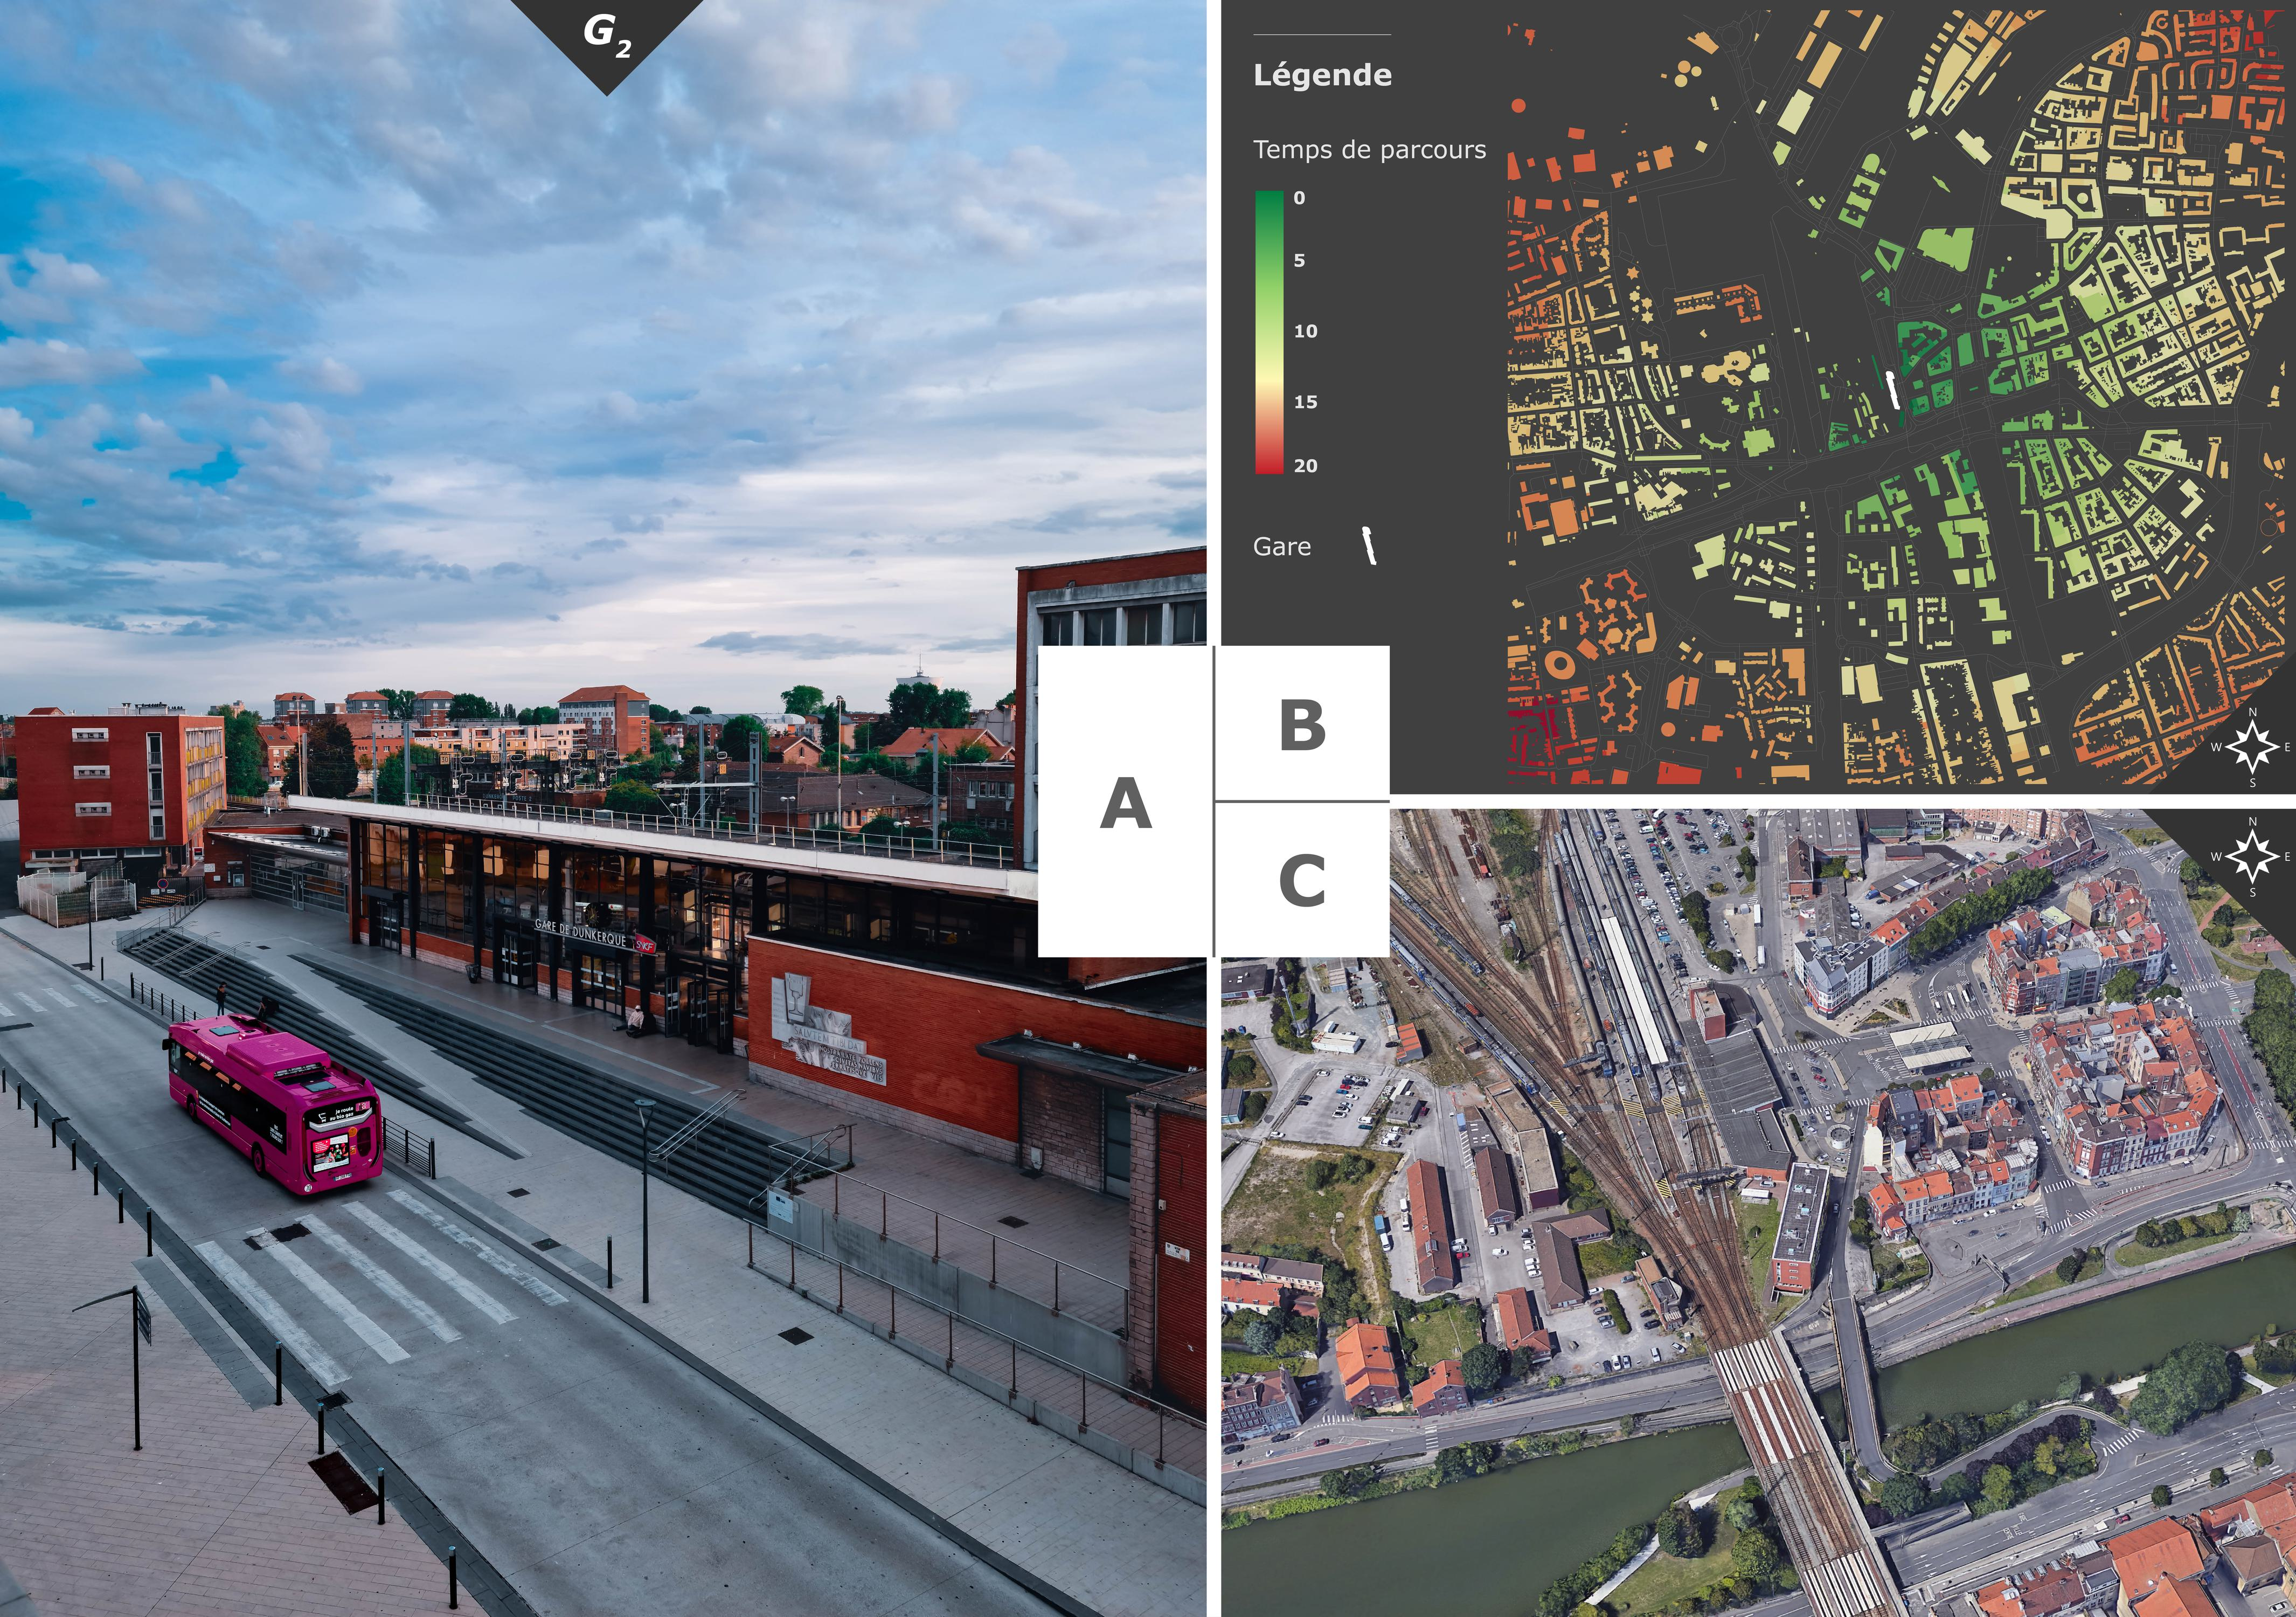
\includegraphics[height=.35\pageheight]{src/Figures/Chap-3/FR_Gare_Dunkerque.jpg}}
        \vspace{5pt}
        \begin{flushright}\scriptsize{
        Photographie (A)~: \textcolor{blue}{Dylan Moinse (2022)}
        \\
        Auteur (B)~: \textcolor{blue}{Dylan Moinse (2024)} avec les données issues d'\textcolor{blue}{\textcite{openstreetmap_openstreetmap_2023}}
        \\
      Jeux de données (C)~: données satellitaires issues de \textcolor{blue}{\textcite{google_earth_google_2023}}
      }\end{flushright}
      \end{carte}

    % Gare Dunkerque (G2)
Parcourue par 2~042~446 voyageur·se·s en 2023 \textcolor{blue}{\autocite{sncf_frequentation_2024}}\index{SNCF@\textsl{SNCF}|pagebf}, la gare de Dunkerque (\(G_2\)) a été sélectionnée pour son rayonnement régional, à la fois pour ses flux ferroviaires et pour son attractivité économique et résidentielle (voir la \hyperref[fig-chap3:monographie-dunkerque]{carte~\ref{fig-chap3:monographie-dunkerque}}, page~\pageref{fig-chap3:monographie-dunkerque}). En nous référant à la typologie des pôles d'échange multimodaux établie dans le \acrshort{SRADDET} de la \textcolor{blue}{\textcite[81]{region_hauts-de-france_sraddet_2024}}\index{Région Hauts-de-France@\textsl{Région Hauts-de-France}|pagebf}, il s'agit d'un \Guillemets{pôle d'échange multimodal régional}. Classée à la 40\textsuperscript{e} position des gares françaises les plus agréables selon le \textsl{Baromètre de satisfaction client en gare} conduit annuellement par \textcolor{blue}{\textcite{sncf_gares__connexions_barometre_2023}}\index{SNCF Gares \& Connexions@\textsl{SNCF Gares \& Connexions}|pagebf}\footnote{
    Cette étude annuelle, menée sur deux périodes distinctes au cours de l’année, évalue la satisfaction des usager·ère·s en gare en s’appuyant sur sept critères de notation désignés comme les \Guillemets{promesses de service}~: (i) la qualité et la clarté des informations en gare, (ii) la fluidité des déplacements, (iii) la propreté et la sûreté des espaces, (iv) le confort des zones d’attente, (v) la présence ainsi que la qualité des commerces et des services disponibles, (vi) la qualité architecturale des bâtiments-voyageur·se·s et la richesse des animations proposées, et enfin (vii) les initiatives en faveur de la mobilité durable \textcolor{blue}{\autocite{sncf_gares__connexions_barometre_2023}}.
}, la cité de Jean Bart jouit de la gare jugée la plus confortable de la région. La gare est connectée à plusieurs réseaux, dont le \acrshort{TER}, le \acrshort{TGV} en provenance de Paris et le réseau \acrshort{TERGV}\footnote{
    Le \acrfull{TERGV} est un train à grande vitesse géré par les autorités régionales, accessible avec un billet de train régional moyennant un supplément tarifaire, sans réservation ni attribution de place. Ce système domestique représente une première en France, porté par des politiques régionales. Les premières lignes, lancées en 2000, ont permis de relier Lille à Dunkerque, Calais~–~Fréthun et Boulogne-Ville en seulement trente minutes. Devant son succès, la fréquence des services a été augmentée dès l’année suivante. En 2003, une nouvelle ligne \acrshort{TERGV} reliant Lille et Arras a été inaugurée, suivie en 2010 par une extension vers les gares du littoral, notamment Étaples~–~Le Touquet et Rang-du-Fliers~–~Verton~–~Berck. La dernière extension du réseau, réalisée en 2020, permet de desservir la ville d'Amiens via la liaison existante entre Lille et Arras. Depuis 2019, le réseau \acrshort{TERGV} est structuré en trois lignes principales regroupées sous l’appellation \Guillemets{Krono+ GV}.
} en direction de la gare Lille Europe, depuis 2000, et d'Amiens via Arras, depuis 2020 \textcolor{blue}{\autocite[85-86]{bourdin_major_2024}}\index{Bourdin, Alain|pagebf}. Dunkerque bénéficie ainsi d'une rare ligne diamétrale dont Lille n'est pas le terminus. Pour reprendre l'expression de \textcolor{blue}{\textcite[102-103]{chen_wider_2012}}\index{Chen, Chia-Lin|pagebf}\index{Hall, Peter|pagebf}, le développement du \acrshort{TGV} et du \acrshort{TERGV} dans la région a favorisé un \Guillemets{rétrécissement de l'espace-temps} (\textsl{effects of time-space shrinkages}), notamment en faveur de Calais et de Dunkerque. Depuis que l'agglomération est accessible à moins de 30 minutes de Lille, le changement de donne permis par l'arrivée de la grande vitesse a contribué à l'émergence de flux pendulaires symétriques, où certains résident·e·s lillois·e·s se rendent quotidiennement dans les zones d'emploi du Dunkerquois, et réciproquement \textcolor{blue}{\autocite[4]{deroo_deplacements_2008}}\index{Deroo, Éric|pagebf}\index{Smuerzinski, Emmanuelle|pagebf}. Le choix de Dunkerque comme étude de cas est également motivé par la gratuité totale des transports urbains, mise en place par la \acrfull{CUD}, sur son réseau \acrshort{BHNS}. Comprenant 18 lignes de bus conventionnelles, dont 6 lignes \textsl{Chronos}, l'agglomération a été le plus grand laboratoire de la gratuité du transport public entre septembre 2018 et décembre 2023. Cette mesure fait actuellement l'objet de discussions quant à son impact sur la pratique de la marche et du vélo, des débats qui s'inscrivent dans la problématique de notre recherche sur l'usage intermodal de la mobilité individuelle légère\footnote{
    À titre d’exemple, une première étude scientifique sur l’expérience dunkerquoise menée entre 2018 et 2019 indique que 7~\% des utilisateur·rice·s du bus gratuit utilisent moins souvent le vélo, tandis que 11~\% l’utilisent toujours autant et 2~\% davantage. Ces chiffres traduisent un report modal du vélo vers le bus estimé à 11~\% \textcolor{blue}{\autocite[25]{javary_gratuite_2020}}\index{Javary, Claire-Marine|pagebf}\index{Huré, Maxime|pagebf}. Au travers d'un scénario basé sur la simulation multi-agents \textsl{MATSim}, \textcolor{blue}{\textcite[10]{kilani_multimodal_2022}}\index{Kilani, Moez|pagebf}\index{Diop, Ngagne|pagebf}\index{Wolf, Daniel de|pagebf} ont démontré qu'une politique régionale de gratuité, sans condition, des transports en commun dans l'ancien Nord-Pas-de-Calais pourrait entraîner une baisse de 17,5~\% de l’usage du vélo comme effet direct.
} \textcolor{blue}{\autocites[25]{javary_gratuite_2020}[10]{kilani_multimodal_2022}}\index{Javary, Claire-Marine|pagebf}\index{Huré, Maxime|pagebf}\index{Kilani, Moez|pagebf}\index{Diop, Ngagne|pagebf}\index{Wolf, Daniel de|pagebf}. Le quartier de gare immédiat de Dunkerque bénéficie également de nombreux projets de requalification. Parmi les réalisations majeures, citons la création d'un parc à vélo sécurisé sur le parvis, offrant 100 places, la construction d'une passerelle reliant la gare à des réserves foncières en mutation ainsi que l'aménagement d'un pôle loisirs. Nous pouvons de plus évoquer la valorisation des espaces publics en ville, se traduisant par un meilleur partage des voies routières et par la piétonisation des places principales.%%Rédigé%%

    % Carte Béthune (G3)
        \begin{carte}[h!]\vspace*{4pt}
        \caption{Monographie de la gare de Béthune.}
        \label{fig-chap3:monographie-bethune}
        \centerline{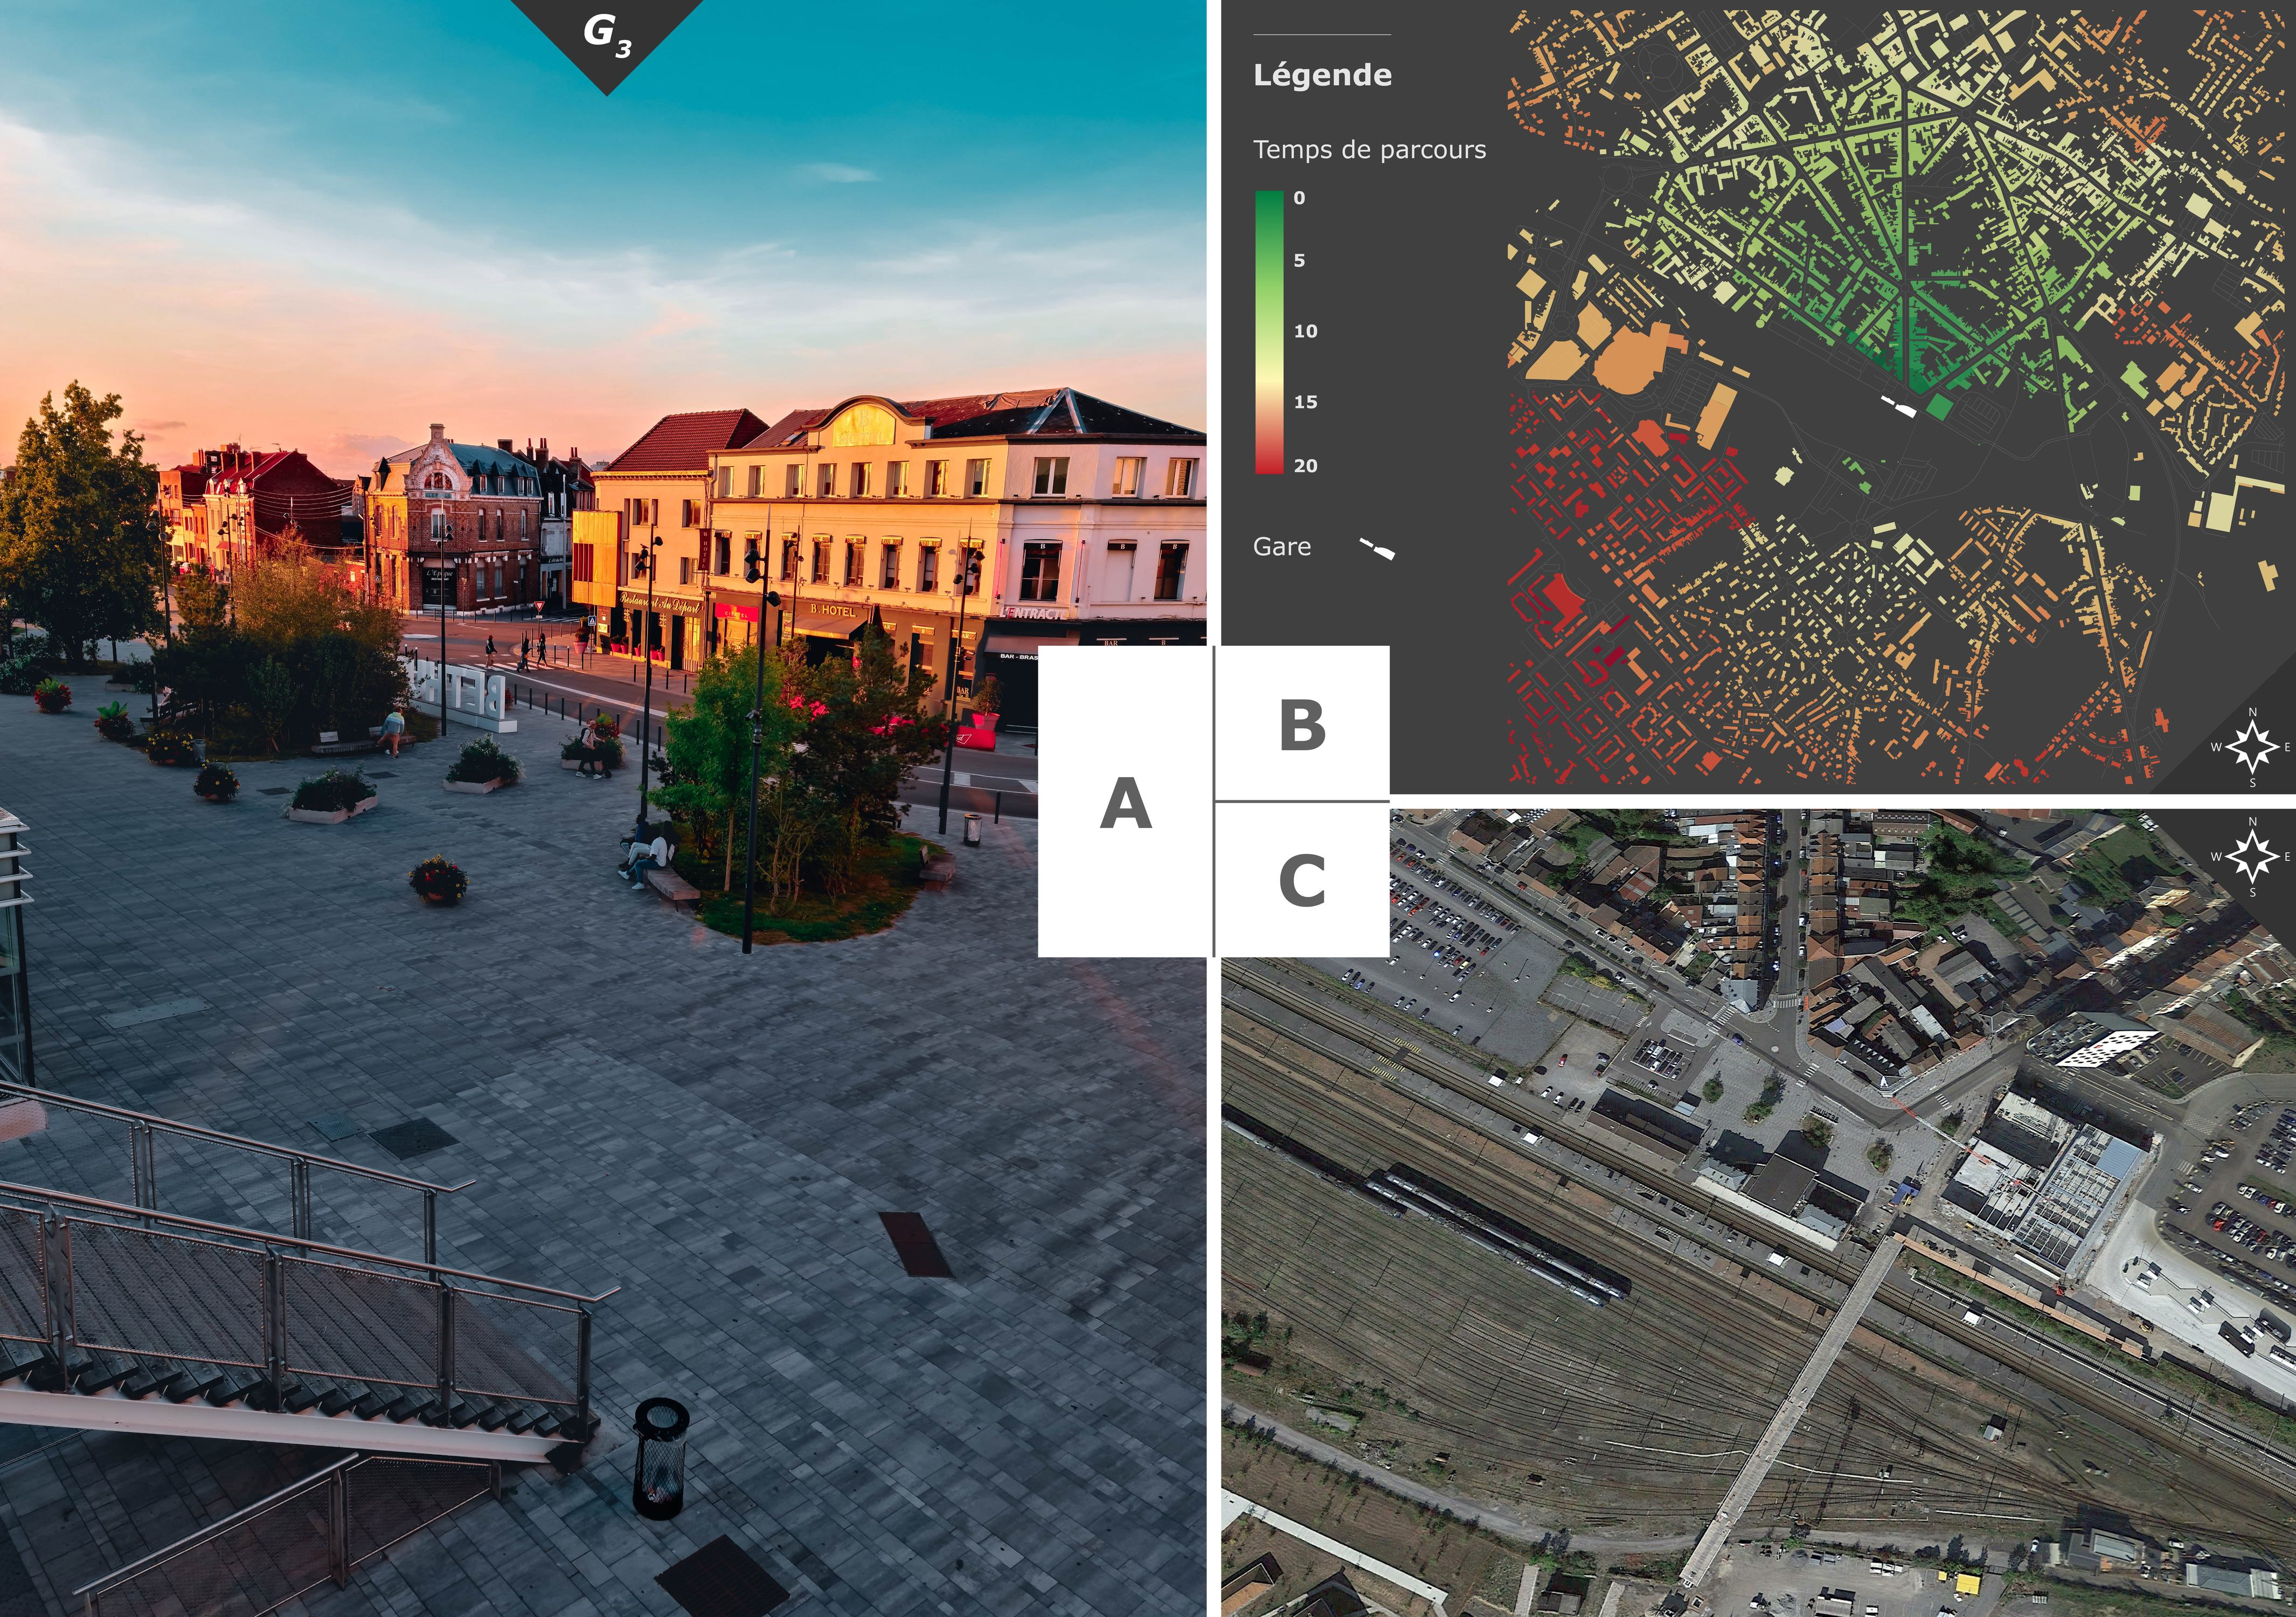
\includegraphics[height=.35\pageheight]{src/Figures/Chap-3/FR_Gare_Bethune.jpg}}
        \vspace{5pt}
        \begin{flushright}\scriptsize{
        Photographie (A)~: \textcolor{blue}{Dylan Moinse (2022)}
        \\
        Auteur (B)~: \textcolor{blue}{Dylan Moinse (2024)} avec les données issues d'\textcolor{blue}{\textcite{openstreetmap_openstreetmap_2023}}
        \\
      Jeux de données (C)~: données satellitaires issues de \textcolor{blue}{\textcite{google_earth_google_2023}}
      }\end{flushright}
      \end{carte}

    % Gare de Béthune (G3)
Avec 1~690~091 voyageur·se·s en 2023 \textcolor{blue}{\autocite{sncf_frequentation_2024}}\index{SNCF@\textsl{SNCF}|pagebf}, la gare de Béthune (\(G_3\)) est un nœud polarisant dans la région, en étant desservie par les réseaux \acrshort{TGV}, sur l'axe reliant Paris à Dunkerque, et \acrshort{TER} (voir la \hyperref[fig-chap3:monographie-bethune]{carte~\ref{fig-chap3:monographie-bethune}}, page~\pageref{fig-chap3:monographie-bethune}). En nous référant à la typologie des pôles d'échange multimodaux établie dans le \acrshort{SRADDET} de la \textcolor{blue}{\textcite[81]{region_hauts-de-france_sraddet_2024}}\index{Région Hauts-de-France@\textsl{Région Hauts-de-France}|pagebf}, il s'agit d'un \Guillemets{pôle d'échange multimodal régional}. Située au cœur du Bassin Minier, deuxième pôle urbain des Hauts-de-France, elle s'insère dans une conurbation dense confrontée à certains enjeux de mobilité. La commune de Béthune fait face à une dépendance automobile marquée. Selon le rapport d'étude produit par la \textcolor{blue}{\textcite[12, 15, 19]{fnaut_deplacements_2022}}\index{Fnaut@\textsl{Fnaut}|pagebf}, 85~\% des déplacements pendulaires des résident·e·s sont effectués en voiture particulière, contre seulement 2~\% à vélo (loin des 8~\% prévus par le \acrshort{PDU} local). En matière d'usage de l'automobile, du transport public ou de la marche, elle figure systématiquement parmi les dernières des 47 plus grandes villes françaises, avec par exemple 4~\% des déplacements réalisés en transport en commun. Tout comme Lens et Douai, Béthune affiche une relation atypique entre sa densité urbaine et la part modale de la voiture, en dépit de la courbe de corrélation inverse très nette que suivent les autres territoires du pays \textcolor{blue}{\autocite[45]{fnaut_deplacements_2022}}\index{Fnaut@\textsl{Fnaut}|pagebf}. Pour répondre à ces défis, plusieurs trajectoires ont marqué le paysage récent des politiques de mobilité du territoire. En premier lieu, le déploiement expérimental d'un système de \acrshort{VFF}, avec l'entreprise \Marque{Bik'air}, à partir de juin 2021, opération qui s'est achevée en décembre 2023. La seconde mesure prend la forme d'une subvention pour l'achat de cycles~: le \textsl{Pass' Mobilité}, mis en place dès 2019, offre une réduction de 200~\euro~pour l'acquisition d'un \acrshort{VAE} et de 50~\euro~pour un vélo classique ou une \acrshort{TEP}, une expérimentation qui a été reconduite pour l'année 2025. La gare de Béthune a également bénéficié d'une transformation majeure de son quartier, amorcée avec la création de la \acrfull{ZAC} du Pôle Gare en 2010. Ce projet urbain a donné lieu à la valorisation de son parvis, au déménagement du pôle bus~–~abritant un nouveau système de \acrshort{BHNS}\footnote{
    À noter qu'à partir de janvier 2026, le réseau \textsl{Tadao} sera rendu intégralement gratuit, devenant ainsi le plus grand réseau gratuit du pays.
}, initialement prévu pour accueillir le tramway~–~à l'installation de deux abris vélo sécurisés et à la réhabilitation de la passerelle. Mais également à l'implantation d'un cinéma en annexe de la gare, à l'aménagement de l'écoquartier de l'Horlogerie sur l'ancienne friche Testut, intégrant logements, bureaux et structures sociales, avec une livraison prévue en 2024. Enfin, le projet \textsl{Station B}, en cours, prévoit la création d'espaces de bureaux. Dans un contexte de forte demande de logements et de croissance démographique parmi les plus élevées des villes de la région \textcolor{blue}{\autocite[32]{fnau_urbanisme_2008}}\index{Fnau@\textsl{Fnau}|pagebf}\index{Direction générale de l'urbanisme, de l'habitat et de la construction@\textsl{Direction générale de l'urbanisme, de l'habitat et de la construction}|pagebf}, ces interventions reflètent les ambitions locales de promouvoir une politique de \Guillemets{recyclage foncier}, en réinvestissant les friches industrielles \textcolor{blue}{\autocite[38]{artois_mobilites_rapport_2024}}\index{Artois Mobilités@\textsl{Artois Mobilités}|pagebf}\index{AULA@\textsl{AULA}|pagebf}.%%Rédigé%%

    % 3.3.3.3.
    \needspace{1\baselineskip} % Réserve de l'espace
\subsubsection*{Gares d'Armentières et de Creil~: portes d'entrée stratégique des métropoles francilienne et lilloise
    \label{chap3:application-observation-quantitative-armentieres-creil}
    }

    % Carte Armentières (G4)
        \begin{carte}[h!]\vspace*{4pt}
        \caption{Monographie de la gare d'Armentières.}
        \label{fig-chap3:monographie-armentieres}
        \centerline{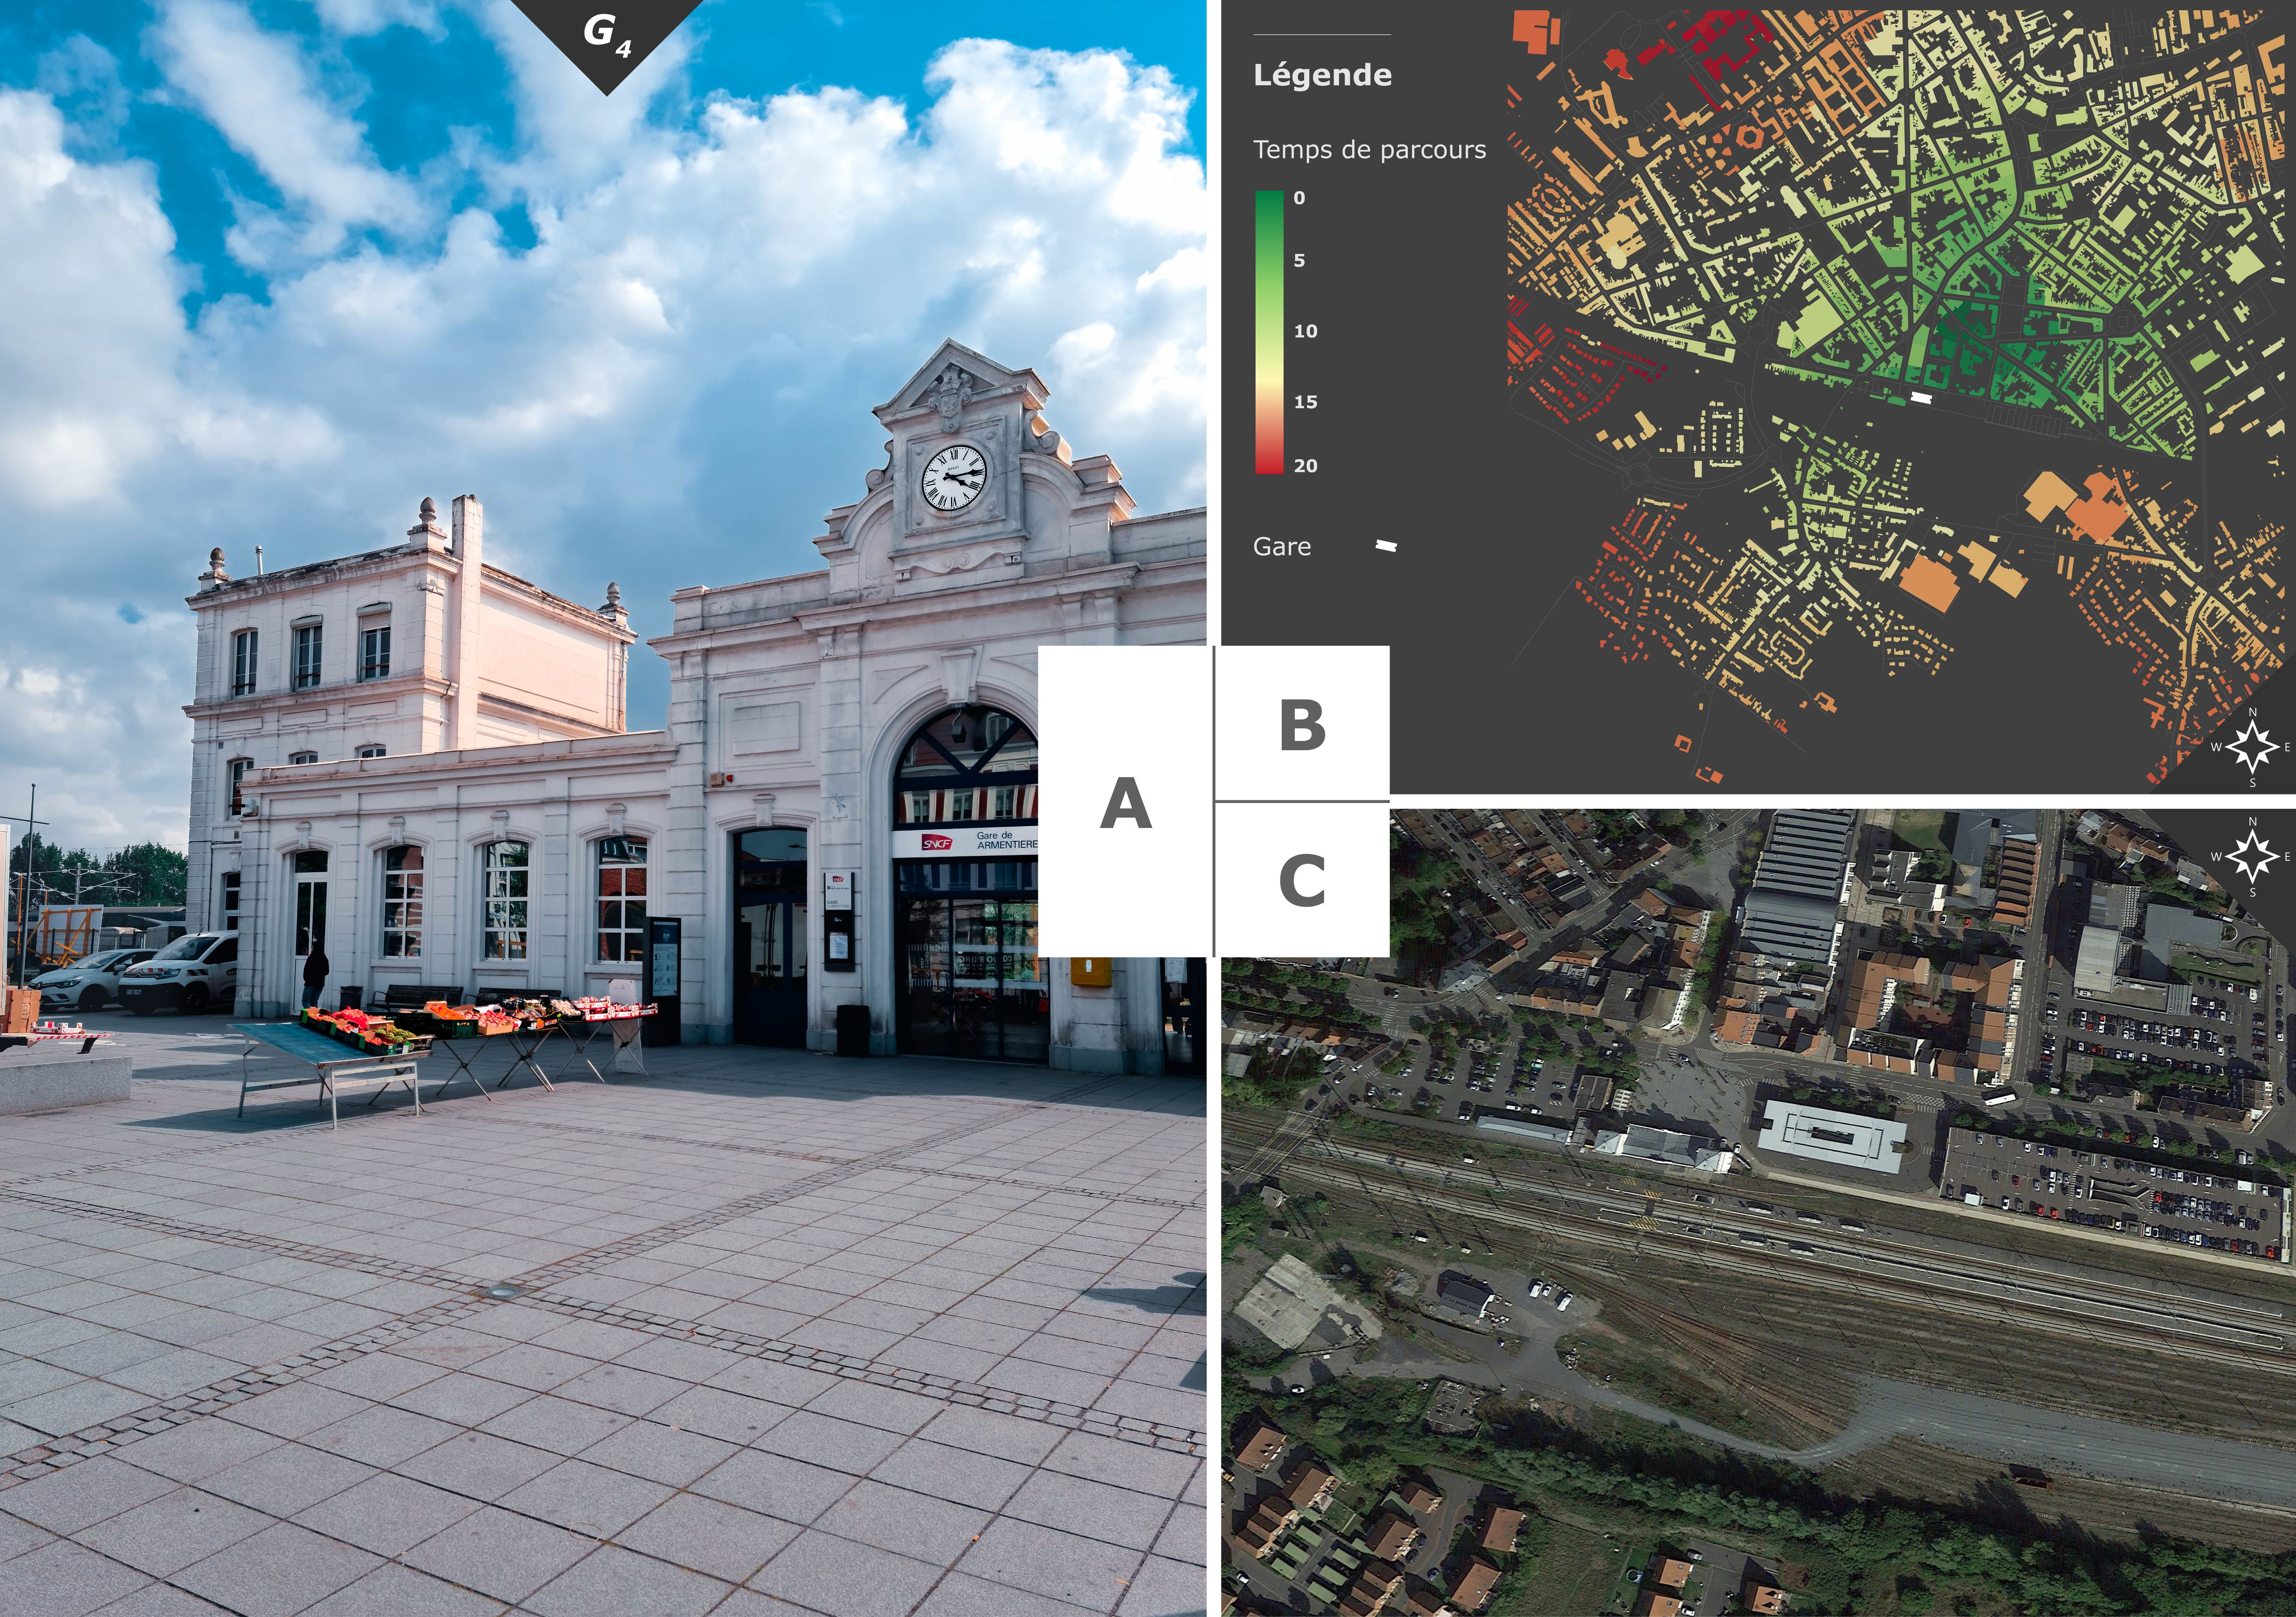
\includegraphics[height=.35\pageheight]{src/Figures/Chap-3/FR_Gare_Armentieres.jpg}}
        \vspace{5pt}
        \begin{flushright}\scriptsize{
        Photographie (A)~: \textcolor{blue}{Dylan Moinse (2022)}
        \\
        Auteur (B)~: \textcolor{blue}{Dylan Moinse (2024)} avec les données issues d'\textcolor{blue}{\textcite{openstreetmap_openstreetmap_2023}}
        \\
      Jeux de données (C)~: données satellitaires issues de \textcolor{blue}{\textcite{google_earth_google_2023}}
      }\end{flushright}
      \end{carte}

    % Gare Armentières (G4)
Deuxième gare du réseau \acrshort{TER} en termes de fréquentation au sein de l'agglomération lilloise, en ayant accueilli 970~659 voyageur·se·s en 2023 \textcolor{blue}{\autocite{sncf_frequentation_2024}}\index{SNCF@\textsl{SNCF}|pagebf}, la gare d’Armentières (\(G_4\)) occupe une position importante dans les territoires périurbains qui structurent la centralité métropolitaine \textcolor{blue}{\autocite[988]{hasiak_can_2021}}\index{Hasiak, Sophie|pagebf}\index{Richer, Cyprien|pagebf}. Ce pôle secondaire, implanté dans une commune de 26~000 habitant·e·s, se situe seulement à 15 minutes de Lille en \acrshort{TER}, assurant une desserte quotidienne allant jusqu’à 90 trains dans chaque sens (voir la \hyperref[fig-chap3:monographie-armentieres]{carte~\ref{fig-chap3:monographie-armentieres}}, page~\pageref{fig-chap3:monographie-armentieres}). En nous référant à la typologie des pôles d'échange multimodaux établie dans le \acrshort{SRADDET} de la \textcolor{blue}{\textcite[82]{region_hauts-de-france_sraddet_2024}}\index{Région Hauts-de-France@\textsl{Région Hauts-de-France}|pagebf}, il s'agit d'un \Guillemets{pôle d'échange multimodal de rabattement vers les métropoles}. Depuis 2006, la gare et son quartier ont fait l'objet d'une profonde transformation, dans le cadre d'un projet de renouvellement urbain \textcolor{blue}{\autocite[90]{schmitt_marches_2020}}\index{Schmitt, Guillaume|pagebf}. Le projet d'aménagement du pôle d'échange multimodal s'inscrit alors dans le premier \acrfull{PDU} de l'ancienne \acrfull{LMCU}, adopté en juin 2000\footnote{
    Ce \acrshort{PDU} métropolitain prévoyait alors la création de sept pôles d'échange, parmi lesquels celui d'Armentières a été inauguré en 2008 \textcolor{blue}{\autocite[90]{schmitt_marches_2020}}\index{Schmitt, Guillaume|pagebf}.
}. Les aménagements réalisés incluent la création de \acrfull{P+R}, d’un \Guillemets{pôle bus-car}, d’un \Guillemets{vélopôle} et la requalification du parvis, libéré du stationnement automobile autrefois participant à l'effet de coupure urbaine \textcolor{blue}{\autocite[53]{christiansen_case_2012}}\index{Christiansen, Petter|pagebf}\index{Eidhammer, Olav|pagebf}\index{Andersen, Jadar|pagebf}\index{L'Hostis, Alain|pagebf}\index{Adamos,~G.|pagebf}\index{Parra,~L.|pagebf}\index{Ruiz-Ayucar,~E.|pagebf}\index{Järvi,~T.|pagebf}\index{Svedova,~Z.|pagebf}\index{Blanquart, Corinne|pagebf}. Des liaisons piétonnes et des voies dédiées au bus ont été aménagées, en même temps qu'un souterrain permettant la traversée des quais. Parallèlement, les friches industrielles environnantes~–~l'ancienne filature Beaudeux, dont l'\acrfull{EPF} a acquis le terrain en 2003, est certainement l'exemple le plus marquant au vu de sa qualité architecturale~–~ont été rénovées ou réhabilitées. Ces projets ont laissé place à des équipements structurants tels que la médiathèque l'Albatros en 2007 et le complexe cinématographique \textsl{Lumières} en 2014, ou encore le programme mixte de commerces, de bureaux et de logements collectifs \textsl{Villas Lumières} la même année \textcolor{blue}{\autocites[5]{richer_reamenagement_2013}[125, 129]{liu_transport_2014}}\index{Richer, Cyprien|pagebf}\index{CETE Nord Picardie@\textsl{CETE Nord Picardie}|pagebf}\index{Liu, Liu|pagebf}\index{L'Hostis, Alain|pagebf}. Le parking silo, doté de 450 places gratuites, a rapidement atteint un taux de remplissage de 90~\% \textcolor{blue}{\autocite[53]{christiansen_case_2012}}\index{Christiansen, Petter|pagebf}\index{Eidhammer, Olav|pagebf}\index{Andersen, Jadar|pagebf}\index{L'Hostis, Alain|pagebf}\index{Adamos,~G.|pagebf}\index{Parra,~L.|pagebf}\index{Ruiz-Ayucar,~E.|pagebf}\index{Järvi,~T.|pagebf}\index{Svedova,~Z.|pagebf}\index{Blanquart, Corinne|pagebf}, encourageant les décideur·se·s et les aménageur·se·s à répondre à cette demande croissante en étendant ce parc relais à 850 places pour les véhicules motorisés et à 66 places sécurisées pour les vélos. La gare d'Armentières s'affiche aujourd'hui comme un pôle intermodal majeur dans la région. Elle se distingue par son interface urbaine dense et dynamique démographiquement, en contraste avec d’autres pôles d’échange comme la gare de Don-Sainghin \textcolor{blue}{\autocite[93]{schmitt_marches_2020}}\index{Schmitt, Guillaume|pagebf}.%%Rédigé%%

    % Carte Creil (G5)
        \begin{carte}[h!]\vspace*{4pt}
        \caption{Monographie de la gare de Creil.}
        \label{fig-chap3:monographie-creil}
        \centerline{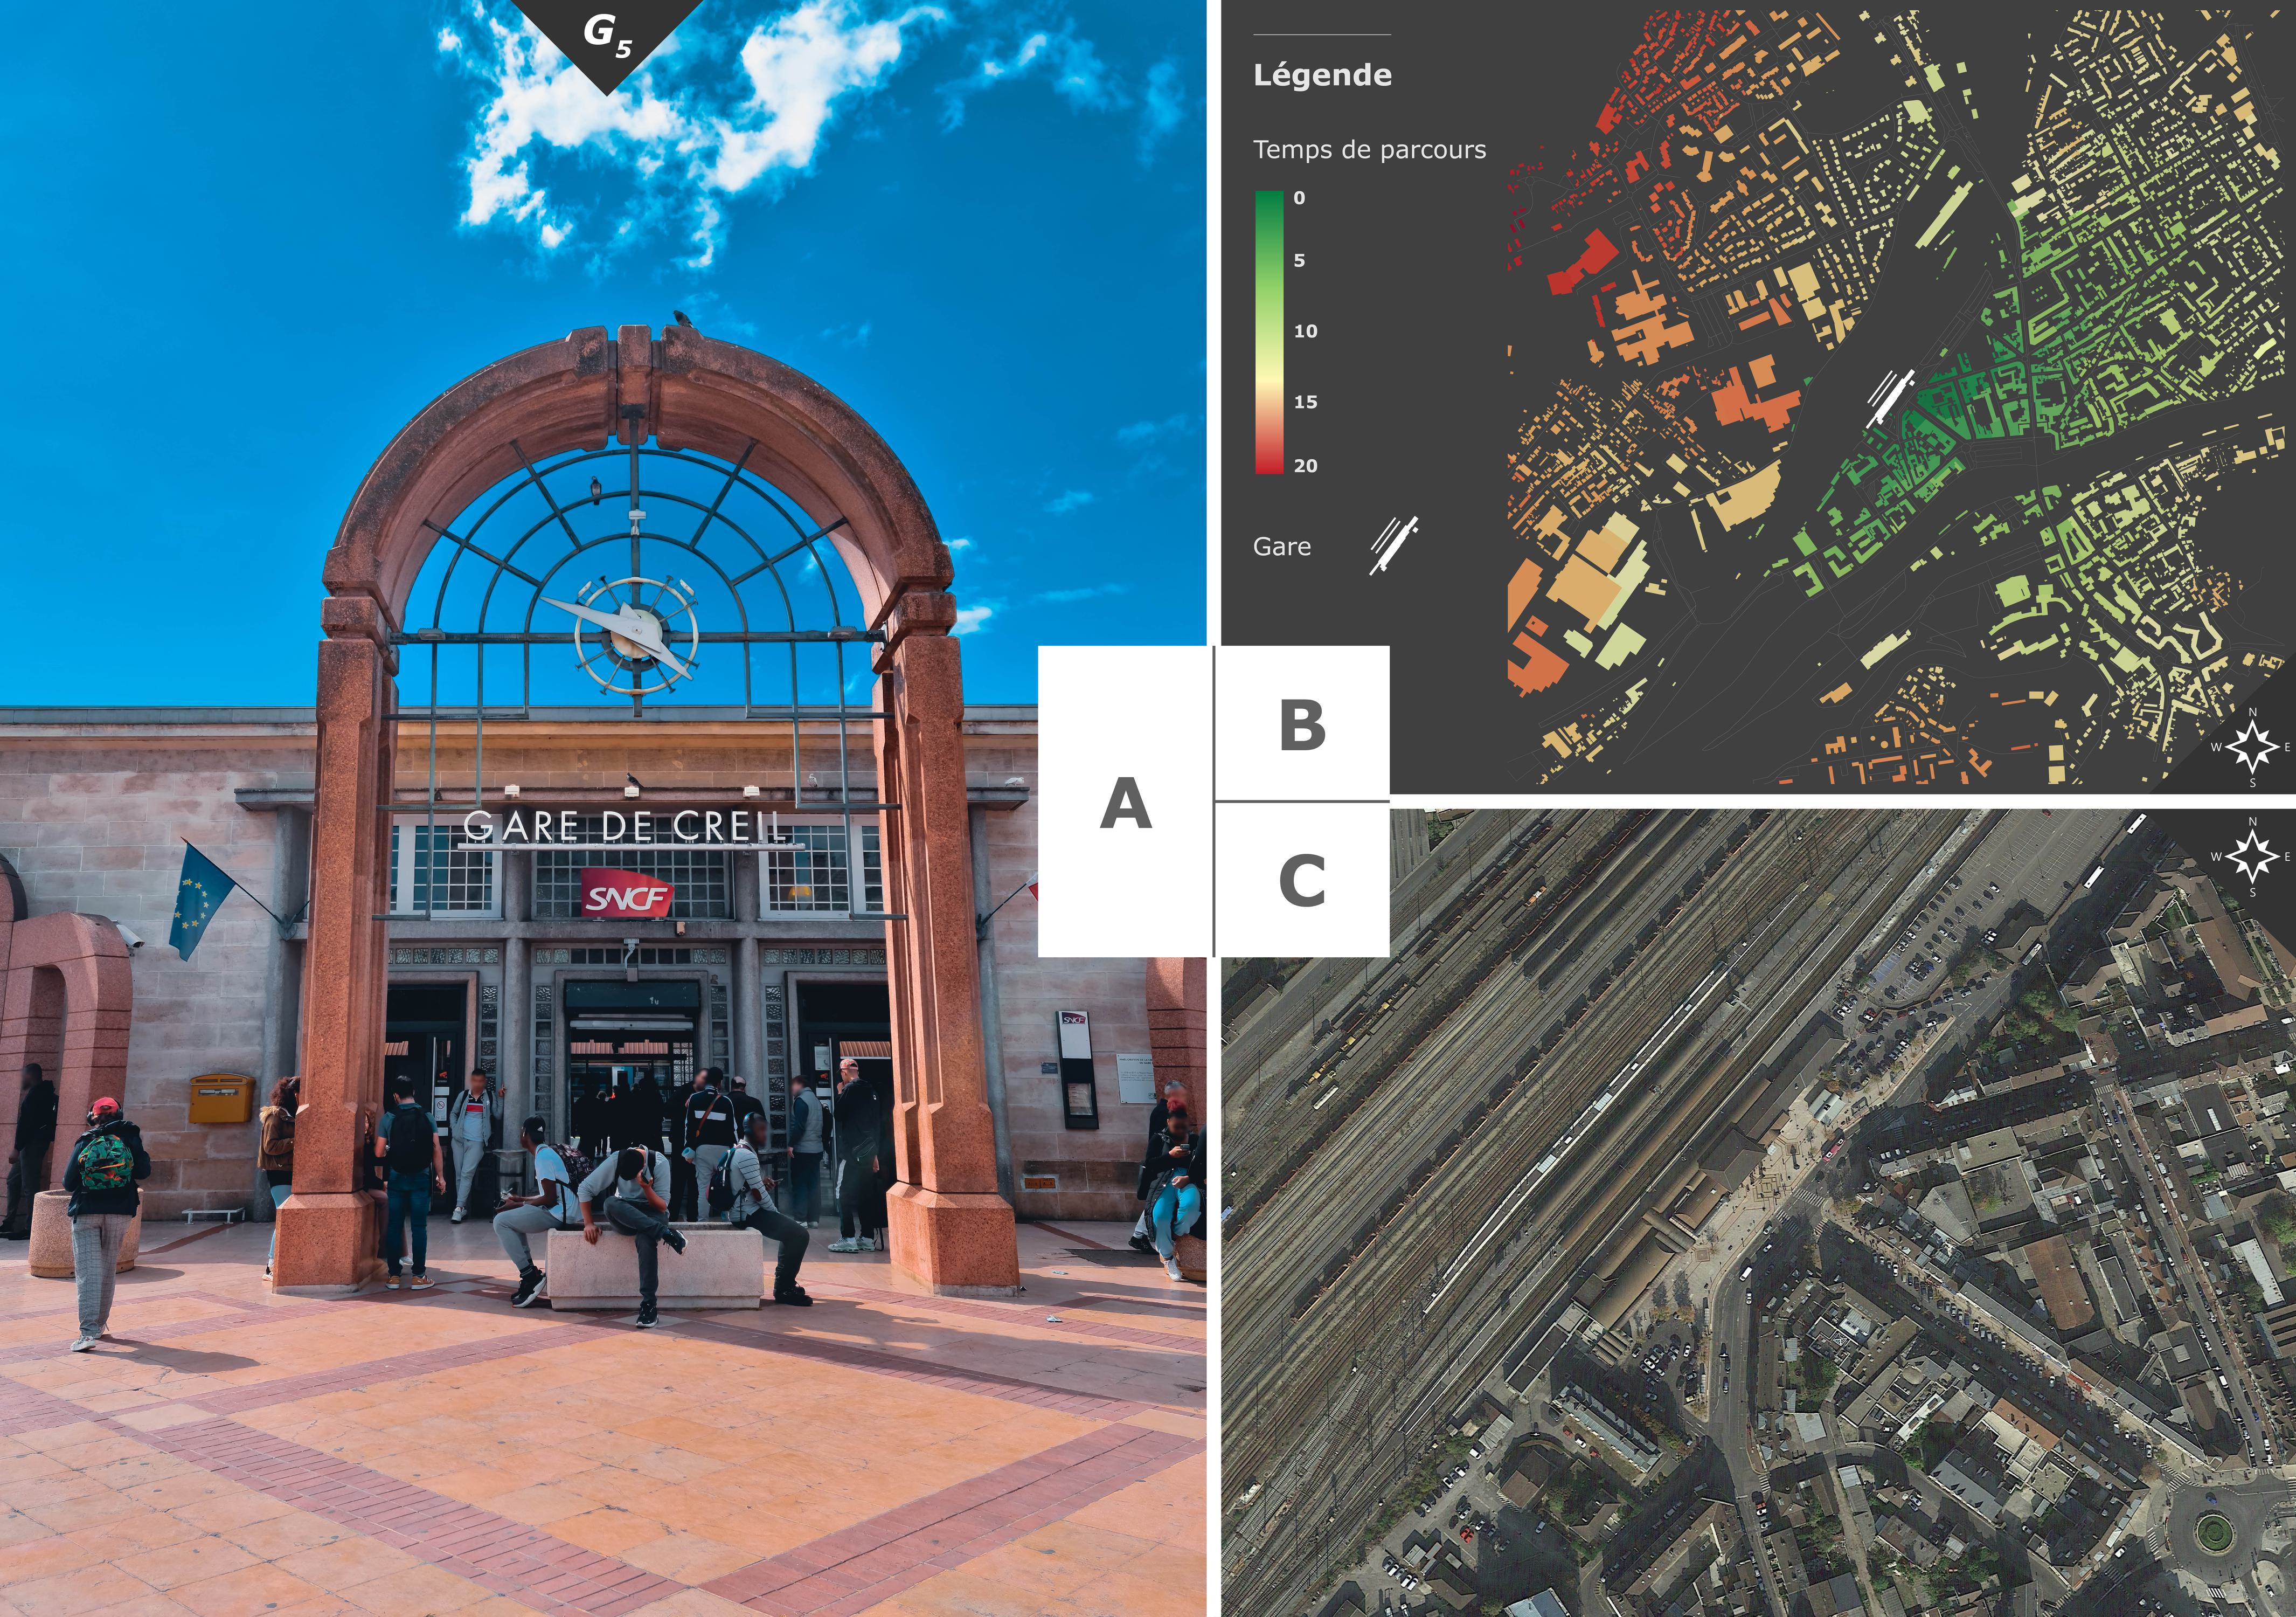
\includegraphics[height=.35\pageheight]{src/Figures/Chap-3/FR_Gare_Creil.jpg}}
        \vspace{5pt}
        \begin{flushright}\scriptsize{
        Photographie (A)~: \textcolor{blue}{Dylan Moinse (2022)}
        \\
        Auteur (B)~: \textcolor{blue}{Dylan Moinse (2024)} avec les données issues d'\textcolor{blue}{\textcite{openstreetmap_openstreetmap_2023}}
        \\
      Jeux de données (C)~: données satellitaires issues de \textcolor{blue}{\textcite{google_earth_google_2023}}
      }\end{flushright}
      \end{carte}

    % Gare Creil (G5)
Fréquentée par 5~392~059 voyageur·se·s en 2023 \textcolor{blue}{\textcite{sncf_frequentation_2024}}\index{SNCF@\textsl{SNCF}|pagebf}, la gare de Creil (\(G_5\)) s'impose comme une infrastructure clé pour l'agglomération francilienne (voir la \hyperref[fig-chap3:monographie-creil]{carte~\ref{fig-chap3:monographie-creil}}, page~\pageref{fig-chap3:monographie-creil}). En nous référant à la typologie des pôles d'échange multimodaux établie dans le \acrshort{SRADDET} de la \textcolor{blue}{\textcite[82]{region_hauts-de-france_sraddet_2024}}\index{Région Hauts-de-France@\textsl{Région Hauts-de-France}|pagebf}, il s'agit d'un \Guillemets{pôle d'échange multimodal de rabattement vers les métropoles}. Première gare de l’ancienne région Picardie en termes d'affluence, devant celle d’Amiens, cette porte d'entrée dans la métropole francilienne \textcolor{blue}{\autocite[166]{lo_feudo_scenario_2014}}\index{Lo Feudo, Fausto|pagebf}\index{Menerault, Philippe|pagebf}\index{L'Hostis, Alain|pagebf}\index{Festa, Demetrio Carmine|pagebf}, qualifiée de \Guillemets{sous-dimensionnée} \textcolor{blue} par l'ancien {\textcite[6]{conseil_regional_de_picardie_gare_2010}}\index{Conseil Régional de Picardie@\textsl{Conseil Régional de Picardie}|pagebf} est desservie par 267 trains quotidiens. Elle accueille les réseaux \acrshort{TER}, la ligne D du \acrshort{RER}, la ligne H du Transilien, et depuis le 19 décembre 2024, les trains Ouigo Train Classique reliant Paris à Bruxelles. Bien qu’elle soit située en dehors de la région administrative francilienne, la gare de Creil est fortement dépendante de l’agglomération parisienne en raison des flux massifs de navetteur·se·s \textcolor{blue}{\autocite[19]{block_novel_2024}}\index{Block, Greet de|pagebf}\index{Blondia, Matthias|pagebf}\index{Cruz, Carla|pagebf}\index{Buldeo Rai, Lisa|pagebf}\index{El Khawand, Maya|pagebf}\index{Vauterin, Leon|pagebf}\index{La Rota, Sandra|pagebf}. Ces flux sont particulièrement marqués sur les branches de l’étoile ferroviaire de Creil, reflet de l’influence de Paris sur l'accès à l'emploi \textcolor{blue}{\autocite[24]{cete_nord_picardie_pour_2011}}\index{CETE Nord Picardie@\textsl{CETE Nord Picardie}|pagebf}. La gare, en tant que point nodal de l’accessibilité régionale, est d'autant plus appelée à renforcer son influence avec le développement de la future liaison ferroviaire Roissy-Picardie\footnote{
    En 2026, une nouvelle voie de 6,5 kilomètres viendra raccorder la ligne ferroviaire Paris à Amiens via Creil, à la gare Aéroport Charles de Gaulle 2 TGV \textcolor{blue}{\autocite{mateos_nouvelle_2024}}\index{Mateos, Frédéric|pagebf}. La gare de Creil sera ainsi directement connectée à l'aéroport, favorisant alors l'intermodalité air-fer, mais également, par correspondance avec le \acrshort{TGV}, à d'autres métropoles françaises telles que Lyon, Marseille ou Strasbourg.
}. En dépit d'une offre ferroviaire remarquable, l’accessibilité à la gare demeure limitée à la centralité immédiate de la ville, en raison de l’étendue de son emprise ferroviaire, qui engendre des ruptures urbaines \textcolor{blue}{\autocite[19]{block_novel_2024}}\index{Block, Greet de|pagebf}\index{Blondia, Matthias|pagebf}\index{Cruz, Carla|pagebf}\index{Buldeo Rai, Lisa|pagebf}\index{El Khawand, Maya|pagebf}\index{Vauterin, Leon|pagebf}\index{La Rota, Sandra|pagebf}. Ce faisceau ferré fragmente en effet l’\acrshort{ACSO}, limitant la connectivité entre Creil et les communes voisines comme Nogent-sur-Oise. En conséquence, un projet de couture urbaine prévoit la construction d'une passerelle ferroviaire de 200 mètres qui sera opérationnelle d’ici à 2029, tout en ajoutant une entrée au nord de la gare qui deviendra dès lors bicéphale \textcolor{blue}{\autocite[6]{conseil_regional_de_picardie_gare_2010}}\index{Conseil Régional de Picardie@\textsl{Conseil Régional de Picardie}|pagebf}.%%Rédigé%%

    % 3.3.3.4.
    \needspace{1\baselineskip} % Réserve de l'espace
\subsubsection*{Halte Lille CHR~: espace nodal stratégique d'accès à l'emploi et de rabattement
    \label{chap3:application-observation-quantitative-lille-chr}
    }

    % Carte Lille CHR (G6)
        \begin{carte}[h!]\vspace*{4pt}
        \caption{Monographie de la halte Lille CHR.}
        \label{fig-chap3:monographie-lille-chr}
        \centerline{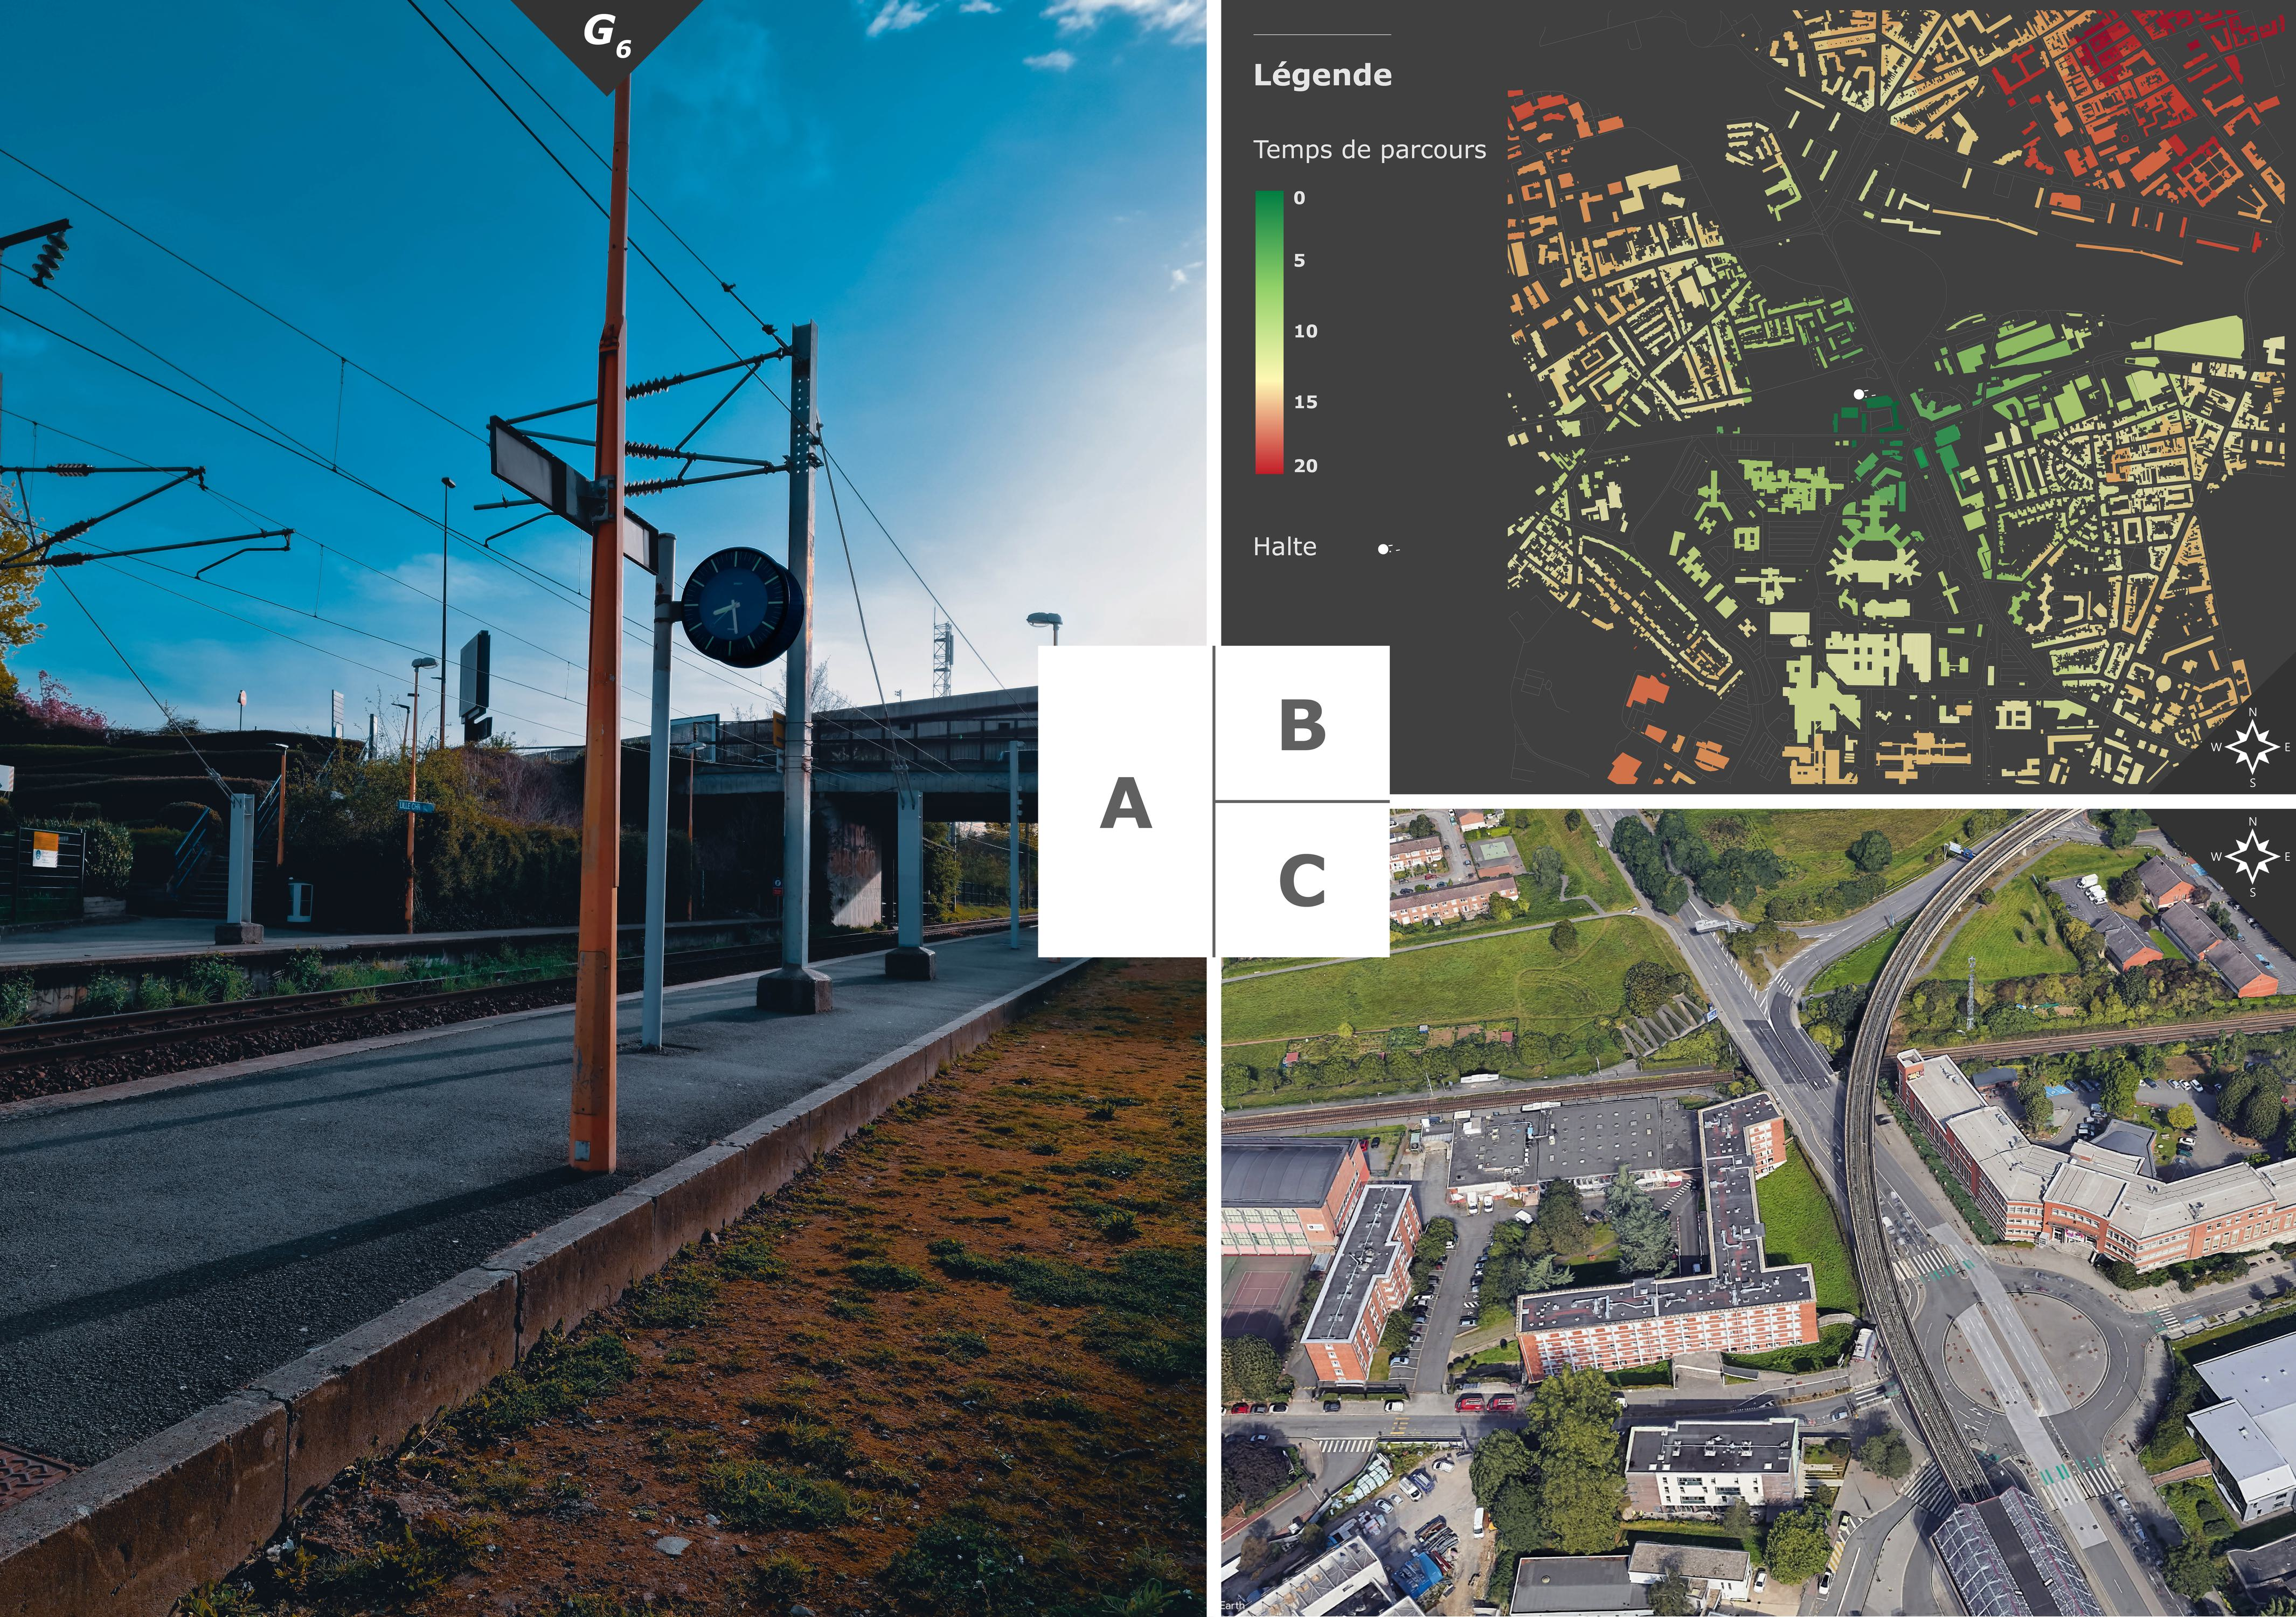
\includegraphics[height=.35\pageheight]{src/Figures/Chap-3/FR_Gare_Lille_CHR.jpg}}
        \vspace{5pt}
        \begin{flushright}\scriptsize{
        Photographie (A)~: \textcolor{blue}{Dylan Moinse (2022)}
        \\
        Auteur (B)~: \textcolor{blue}{Dylan Moinse (2024)} avec les données issues d'\textcolor{blue}{\textcite{openstreetmap_openstreetmap_2023}}
        \\
      Jeux de données (C)~: données satellitaires issues de \textcolor{blue}{\textcite{google_earth_google_2023}}
      }\end{flushright}
      \end{carte}

    % Halte Lille CHR (G6)
Avec une fréquentation de 349~246 voyageur·se·s en 2023 \textcolor{blue}{\autocite{sncf_frequentation_2024}}\index{SNCF@\textsl{SNCF}|pagebf}, la halte Lille CHR (\(G_6\)) constitue à juste titre une autre configuration de \Guillemets{porte d'entrée} stratégique au sein de l'agglomération lilloise \textcolor{blue}{\autocite[144]{menerault_recherche_2020}}\index{Menerault, Philippe|pagebf}\index{Richer, Cyprien|pagebf}. Bénéficiant d’une desserte quotidienne de 64 \acrshort{TER} en provenance de Béthune, de Lens et de Saint-Pol-sur-Ternoise, elle profite d'une connexion à proximité avec la station de métro CHU~–~Centre Oscar-Lambret (ligne~1) et offre ainsi un accès privilégié à certains secteurs centraux lillois~–~tels Wazemmes, Gambetta et République~–~Beaux-Arts~–~sans nécessiter de correspondance par la gare centrale (voir la \hyperref[fig-chap3:monographie-lille-chr]{carte~\ref{fig-chap3:monographie-lille-chr}}, page~\pageref{fig-chap3:monographie-lille-chr}). En nous référant à la typologie des pôles d'échange multimodaux établie dans le \acrshort{SRADDET} de la \textcolor{blue}{\textcite[83-84]{region_hauts-de-france_sraddet_2024}}\index{Région Hauts-de-France@\textsl{Région Hauts-de-France}|pagebf}, il s'agit d'un \Guillemets{pôle d'entrée urbain} et dans le même temps un \Guillemets{pôle d'interconnexion intra-urbain}. La position stratégique de ce pôle secondaire permet aux voyageur·se·s de contourner la surcharge récurrente des \acrshort{TER} et du métro à Lille Flandres, aux heures de pointe, tout en proposant un parcours plus rapide \textcolor{blue}{\autocite[130]{fleury_gestion_2002}}\index{Fleury, Dominique|pagebf}\index{Brenac, Thierry|pagebf}\index{Derrien, Xavier|pagebf}\index{Fleury, Dominique|pagebf}\index{Frère, Séverine|pagebf}\index{Guilbot, Michèle|pagebf}\index{Hernandez, Frédérique|pagebf}\index{Menerault, Philippe|pagebf}\index{Millot, Marine|pagebf}\index{Pysson, Sylvie|pagebf}\index{Reigner, Hélène|pagebf}\index{Yerpez, Joël|pagebf}. Une analyse multicritère des gares de la région permet alors de désigner la halte Lille CHR comme un exemple de \textsl{congruence nodale} \textcolor{blue}{\autocite[129]{fleury_gestion_2002}}\index{Fleury, Dominique|pagebf}\index{Brenac, Thierry|pagebf}\index{Derrien, Xavier|pagebf}\index{Fleury, Dominique|pagebf}\index{Frère, Séverine|pagebf}\index{Guilbot, Michèle|pagebf}\index{Hernandez, Frédérique|pagebf}\index{Menerault, Philippe|pagebf}\index{Millot, Marine|pagebf}\index{Pysson, Sylvie|pagebf}\index{Reigner, Hélène|pagebf}\index{Yerpez, Joël|pagebf}, avec des réseaux juxtaposés plus que complémentaires \textcolor{blue}{\autocite[107]{menerault_gares_2001}}\index{Menerault, Philippe|pagebf}\index{Barré, Alain|pagebf}. Créée en 1996, la halte est initialement conçue pour desservir le Centre Hospitalier Régional après le déplacement de l’ancienne gare de Lille Sud. Cependant, cette infrastructure n'a pas été pensée dans une optique d’interconnexion entre le réseau ferroviaire et le système de \acrfull{VAL}. En cela, elle illustre bien le passage d’une \Guillemets{\textsl{interconnexion qui s’ignore}} à une \Guillemets{\textsl{interconnexion qui se cherche}}, selon les termes de \textcolor{blue}{\textcite[109]{barre_interconnexion_2001}}\index{Barré, Alain|pagebf}\index{Menerault, Philippe|pagebf}. Les proximités spatiales entre les deux points d'arrêt, renforcées par la visibilité directe du viaduc du métro à la sortie de la halte, témoignent d’un potentiel encore sous-valorisé \textcolor{blue}{\autocite[130]{fleury_gestion_2002}}\index{Fleury, Dominique|pagebf}\index{Brenac, Thierry|pagebf}\index{Derrien, Xavier|pagebf}\index{Fleury, Dominique|pagebf}\index{Frère, Séverine|pagebf}\index{Guilbot, Michèle|pagebf}\index{Hernandez, Frédérique|pagebf}\index{Menerault, Philippe|pagebf}\index{Millot, Marine|pagebf}\index{Pysson, Sylvie|pagebf}\index{Reigner, Hélène|pagebf}\index{Yerpez, Joël|pagebf}~: cette halte bénéficie aujourd’hui d’une bonne intégration grâce à des cheminements piétonniers qui facilitent l’articulation entre le réseau ferré et le réseau de transport urbain, mais la signalétique et la communication ne garantissent pas une information-voyageur·se·s optimale. Sur le plan urbain, la gare Lille CHR est déterminante dans la desserte du parc Eurasanté, situé au cœur du campus hospitalo-universitaire du CHU de Lille, en cours de développement \textcolor{blue}{\autocite[130]{fleury_gestion_2002}}\index{Fleury, Dominique|pagebf}\index{Brenac, Thierry|pagebf}\index{Derrien, Xavier|pagebf}\index{Fleury, Dominique|pagebf}\index{Frère, Séverine|pagebf}\index{Guilbot, Michèle|pagebf}\index{Hernandez, Frédérique|pagebf}\index{Menerault, Philippe|pagebf}\index{Millot, Marine|pagebf}\index{Pysson, Sylvie|pagebf}\index{Reigner, Hélène|pagebf}\index{Yerpez, Joël|pagebf}.%%Rédigé%%

    % 3.3.3.5.
    \needspace{1\baselineskip} % Réserve de l'espace
\subsubsection*{Gare de Lesquin et halte du Poirier Université~: infrastructures de desserte secondaires avec un potentiel d'accès aux équipements
    \label{chap3:application-observation-quantitative-lesquin-poirier-universite}
    }

    % Carte Lesquin (G7)
        \begin{carte}[h!]\vspace*{4pt}
        \caption{Monographie de la gare de Lesquin.}
        \label{fig-chap3:monographie-lesquin}
        \centerline{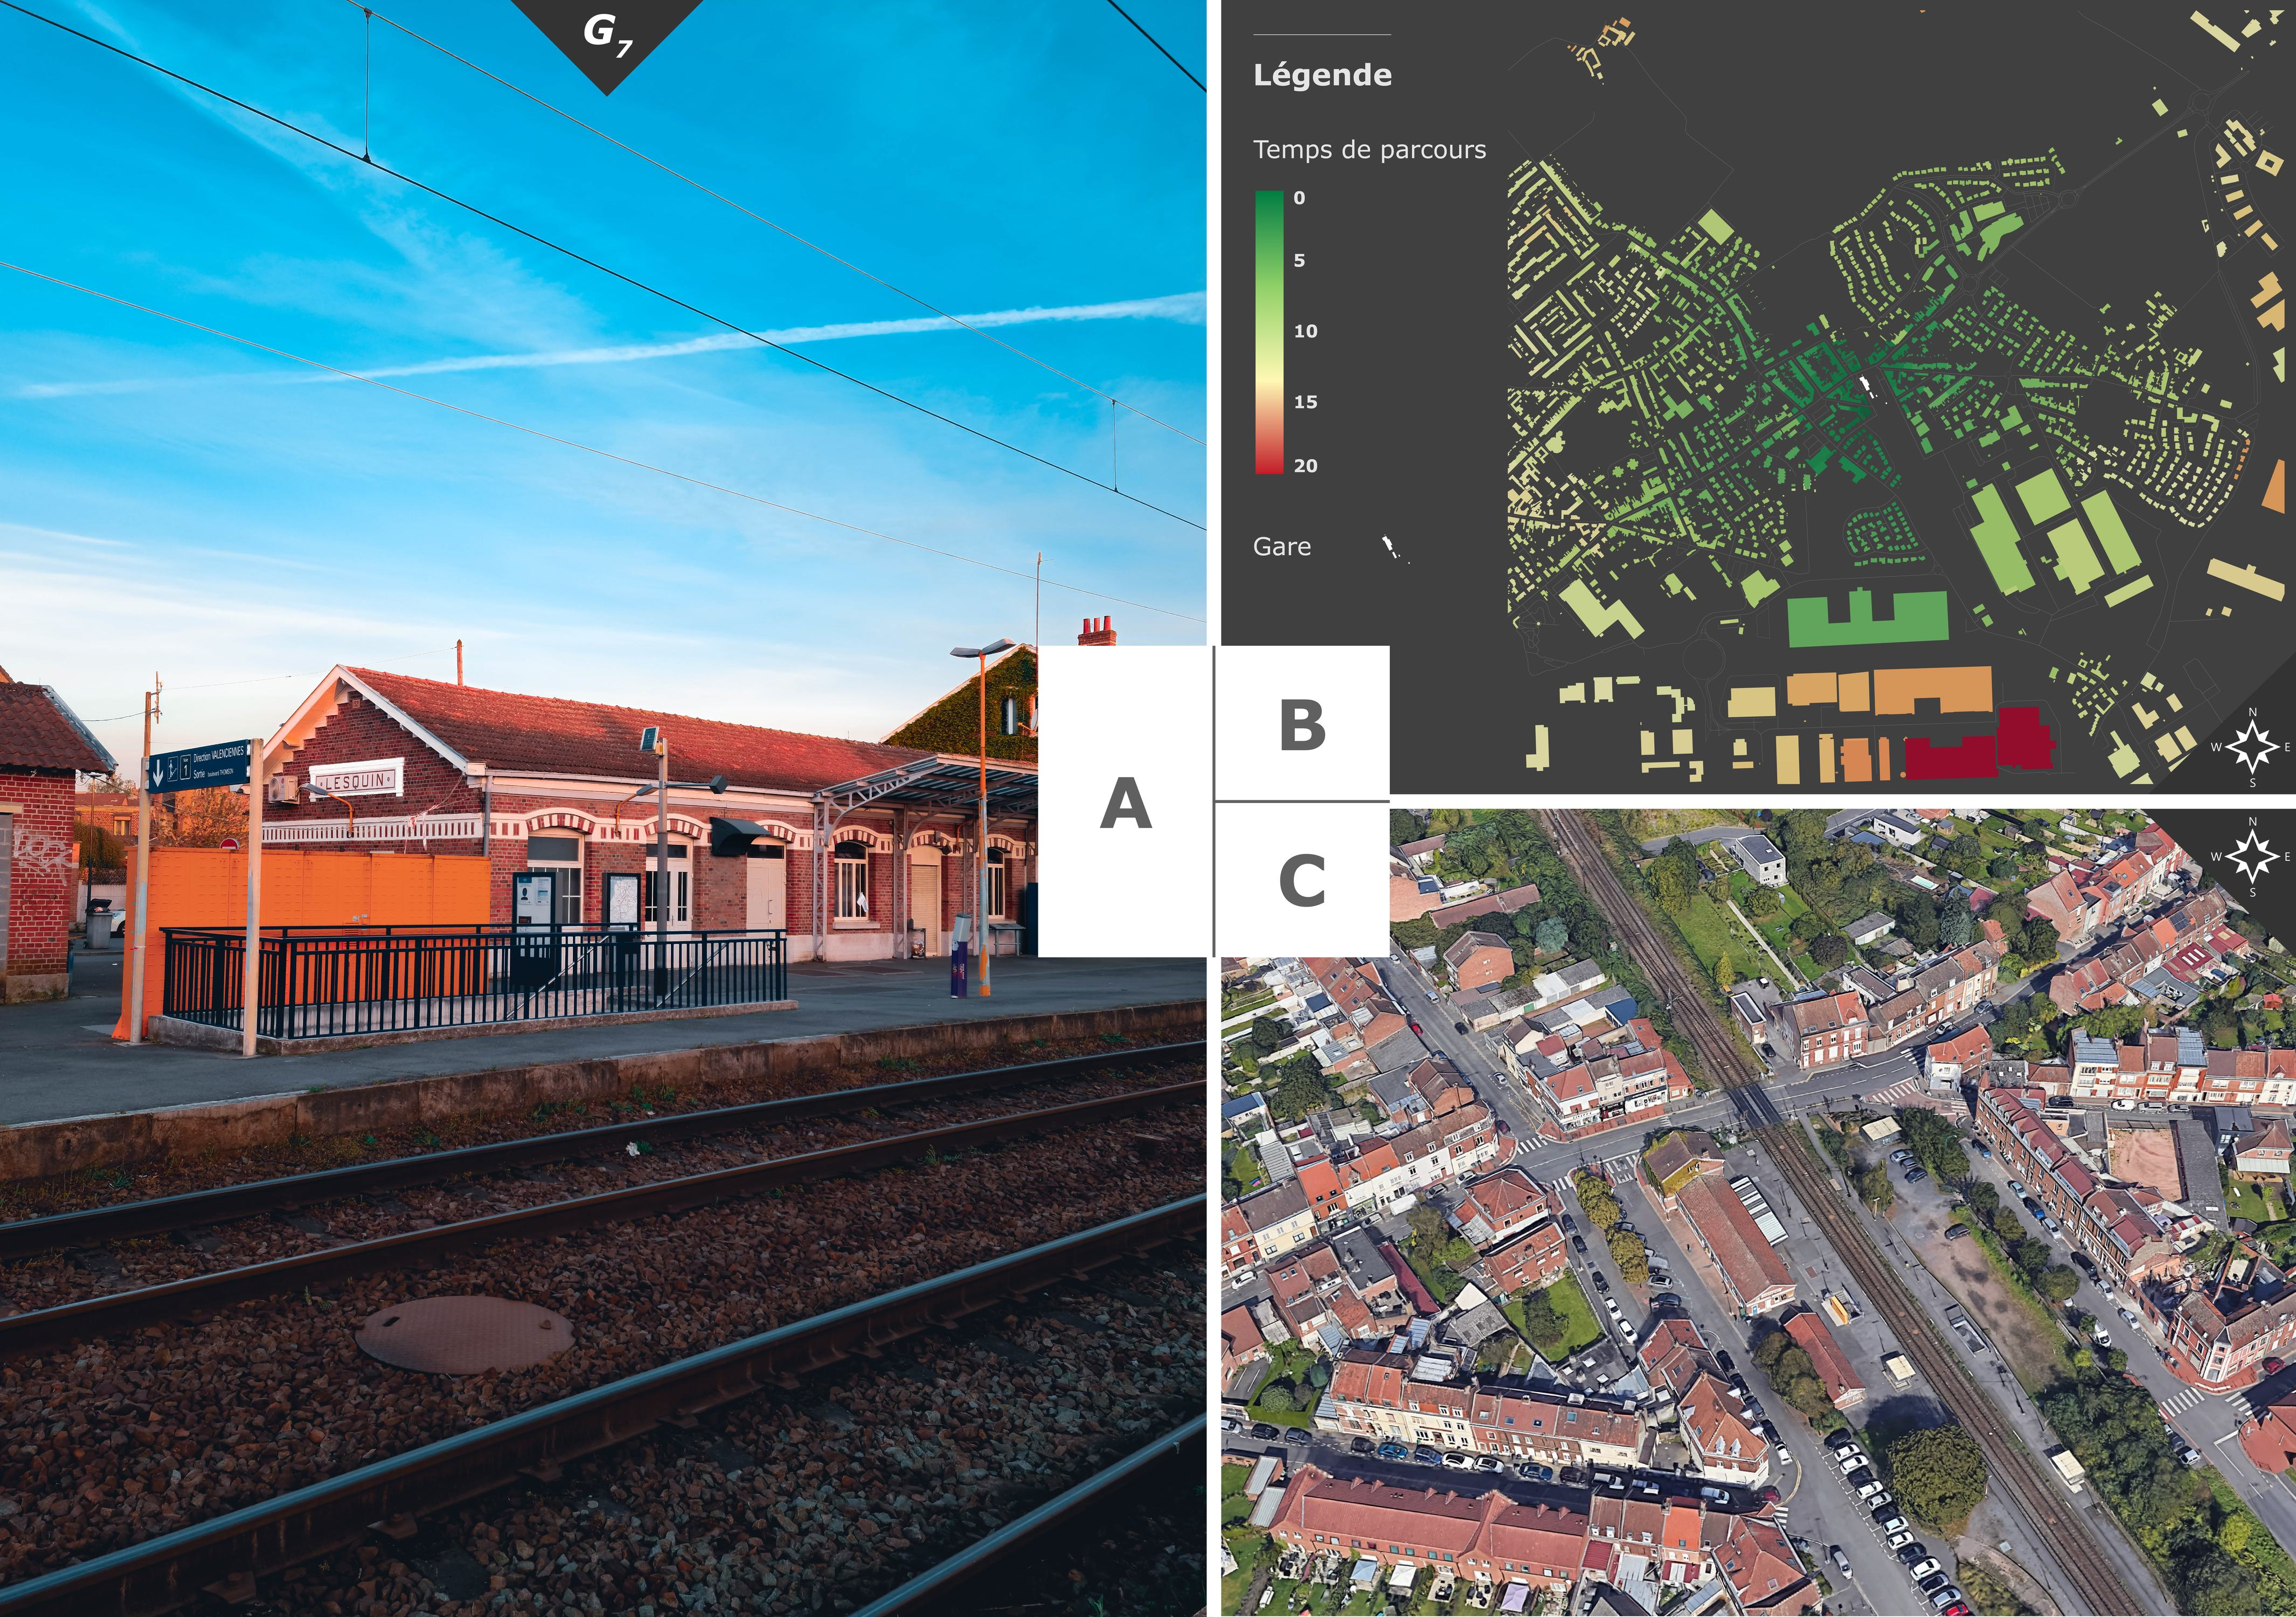
\includegraphics[height=.35\pageheight]{src/Figures/Chap-3/FR_Gare_Lesquin.jpg}}
        \vspace{5pt}
        \begin{flushright}\scriptsize{
        Photographie (A)~: \textcolor{blue}{Dylan Moinse (2022)}
        \\
        Auteur (B)~: \textcolor{blue}{Dylan Moinse (2024)} avec les données issues d'\textcolor{blue}{\textcite{openstreetmap_openstreetmap_2023}}
        \\
      Jeux de données (C)~: données satellitaires issues de \textcolor{blue}{\textcite{google_earth_google_2023}}
      }\end{flushright}
      \end{carte}

    % Gare de Lesquin (G7)
Avec moins de 160~619 voyageur·se·s en 2023 \textcolor{blue}{\autocite{sncf_frequentation_2024}}\index{SNCF@\textsl{SNCF}|pagebf}, la gare de Lesquin (\(G_7\)), située à seulement sept minutes de la gare Lille Flandres en \acrshort{TER}, se positionne comme une gare secondaire (voir la \hyperref[fig-chap3:monographie-lesquin]{carte~\ref{fig-chap3:monographie-lesquin}}, page~\pageref{fig-chap3:monographie-lesquin}). En nous référant à la typologie des pôles d'échange multimodaux établie dans le \acrshort{SRADDET} de la \textcolor{blue}{\textcite[83]{region_hauts-de-france_sraddet_2024}}\index{Région Hauts-de-France@\textsl{Région Hauts-de-France}|pagebf}, il s'agit d'un \Guillemets{pôle relai}. Contrairement à la halte Lille CHR, elle ne bénéficie toutefois ni d’une interconnexion forte avec les réseaux de transport urbain, ni d’une proximité immédiate avec des \acrshort{POIs} métropolitains ou régionaux. Elle constitue néanmoins un arrêt sur l’axe \Guillemets{semi-rapide} en provenance de Valenciennes \textcolor{blue}{\autocite[38]{menerault_analyse_2000}}\index{Menerault, Philippe|pagebf}\index{L'Hostis, Alain|pagebf}, aux côtés des gares de Saint-Amand-les-Eaux, d'Orchies et de Templeuve. L'intérêt de cette gare réside dans son potentiel de connexion avec des équipements majeurs tels que le campus Cité Scientifique de l’Université de Lille et le parc scientifique de la Haute-Borne, un pôle d’excellence métropolitain difficilement connecté au réseau de transport urbain. La gare de Lesquin dispose ainsi d’une accessibilité inexploitée, notamment grâce à des possibilités de connexion entre le réseau ferroviaire, le réseau de bus et le réseau cyclable. Ces opportunités restent pourtant occultées par la logique première du couple train et métro \acrshort{VAL} pour atteindre ces destinations \textcolor{blue}{\autocite[18]{lhostis_definir_2010}}\index{L'Hostis, Alain|pagebf}\index{Conesa, Alexis|pagebf}\index{Arnaud Banos, Thomas Thévenin|pagebf}. En réalité, la gare de Lesquin pourrait s'avérer plus performante en termes de temps de trajet pour relier ces zones depuis les agglomérations de Valenciennes ou de Maubeuge. Par exemple, un trajet en bus, incluant la marche combinée, permet d’atteindre l’École Centrale de Lille entre 10 et 13 minutes, tandis qu’un trajet à vélo depuis la gare prend environ 9 minutes. Ces alternatives offrent environ un quart d'heure d'économies de temps de déplacement par rapport à un \gls{itinéraire} en train et en métro, tout en évitant les saturations fréquentes à la gare Lille Flandres \textcolor{blue}{\autocites[58]{menerault_analyse_2000}[14]{lhostis_definir_2010}}\index{L'Hostis, Alain|pagebf}\index{Conesa, Alexis|pagebf}\index{Arnaud Banos, Thomas Thévenin|pagebf}\index{Menerault, Philippe|pagebf}. Bien que la gare de Lesquin reste peu exploitée, elle se différencie des autres pôles secondaires par les gains de temps tangibles qu'elle offre à certain·e·s usager·ère·s de la ligne. Cette caractéristique souligne son potentiel de valorisation intermodale \textcolor{blue}{\autocite[62]{menerault_analyse_2000}}\index{Menerault, Philippe|pagebf}\index{L'Hostis, Alain|pagebf}. Toutefois, malgré le développement d'infrastructures cyclables reliant la gare au campus et au parc scientifique, ces liaisons souffrent d’un manque de continuité et d'une cohabitation conflictuelle avec les piéton·ne·s le long d’une route métropolitaine à fort trafic motorisé.%%Rédigé%%

    % Carte Le Poirier Université (G8)
        \begin{carte}[h!]\vspace*{4pt}
        \caption{Monographie de la halte du Poirier Université.}
        \label{fig-chap3:monographie-le-poirier}
        \centerline{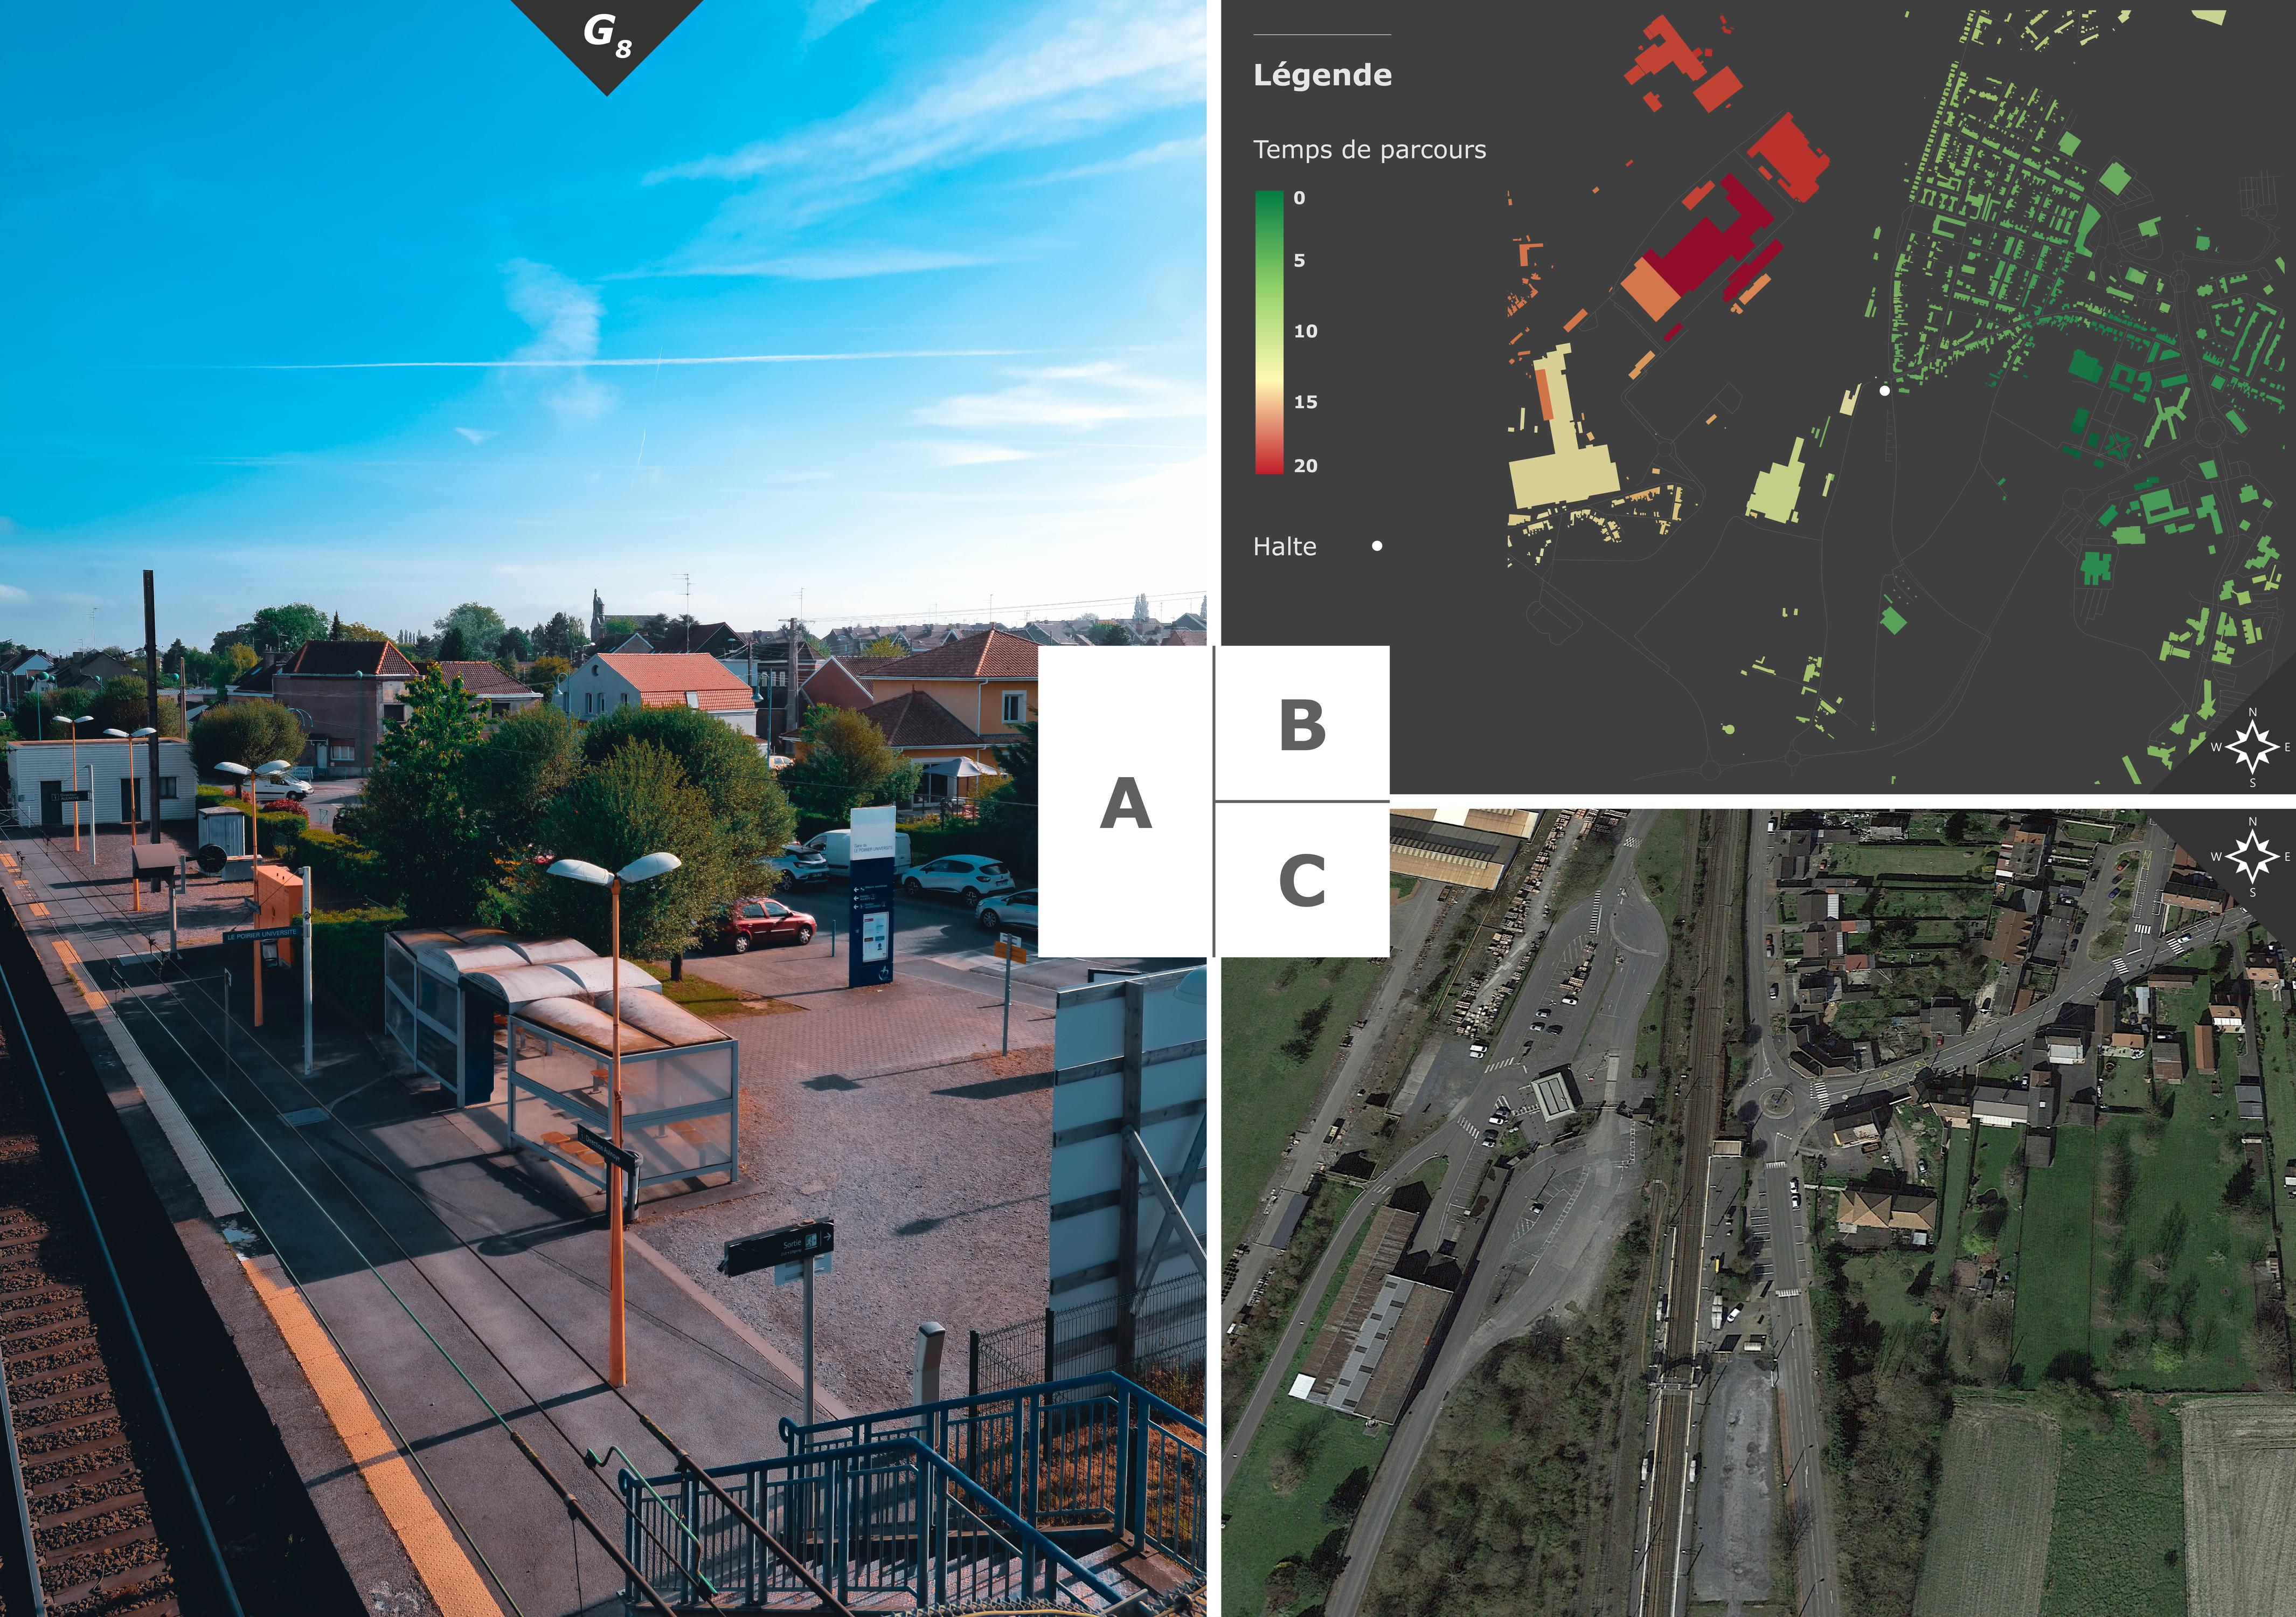
\includegraphics[height=.35\pageheight]{src/Figures/Chap-3/FR_Gare_Poirier.jpg}}
        \vspace{5pt}
        \begin{flushright}\scriptsize{
        Photographie (A)~: \textcolor{blue}{Dylan Moinse (2022)}
        \\
        Auteur (B)~: \textcolor{blue}{Dylan Moinse (2024)} avec les données issues d'\textcolor{blue}{\textcite{openstreetmap_openstreetmap_2023}}
        \\
      Jeux de données (C)~: données satellitaires issues de \textcolor{blue}{\textcite{google_earth_google_2023}}
      }\end{flushright}
      \end{carte}

    % Halte du Poirier Université (G8)
À l’instar de la gare de Lesquin, la halte du Poirier Université (\(G_8\)), traversée par 84~969 voyageur·se·s en 2023 \textcolor{blue}{\autocite{sncf_frequentation_2024}}\index{SNCF@\textsl{SNCF}|pagebf}, se positionne comme une gare secondaire, située à proximité immédiate du campus du Mont Houy, au sein de l’Université Polytechnique Hauts-de-France, à Valenciennes (voir la \hyperref[fig-chap3:monographie-le-poirier]{carte~\ref{fig-chap3:monographie-le-poirier}}, page~\pageref{fig-chap3:monographie-le-poirier}). En nous référant à la typologie des pôles d'échange multimodaux établie dans le \acrshort{SRADDET} de la \textcolor{blue}{\textcite[83]{region_hauts-de-france_sraddet_2024}}\index{Région Hauts-de-France@\textsl{Région Hauts-de-France}|pagebf}, il s'agit d'un \Guillemets{pôle relai}. Pour autant, le \acrshort{PDU} 2013-2023 du Valenciennois considère ce point d'arrêt, parmi les 12 gares qui structurent l'agglomération, de \Guillemets{pôle important} avec celui de la gare de Valenciennes et de Saint-Amand-les-Eaux \textcolor{blue}{\autocite[43-44]{siturv_plan_2014}}\index{SITURV@\textsl{SITURV}|pagebf}. Renommée en 2001 pour refléter cette proximité avec le campus, situé à un kilomètre, cette halte s’intègre dans l’axe ferroviaire reliant Lille à Hirson, via Valenciennes. En ajoutant un trajet de cinq minutes en \acrshort{TER} au départ de la gare de Valenciennes, les voyageur·se·s peuvent accéder à ce point d'arrêt, qui se classe comme la troisième de l’agglomération en termes de fréquentation. Elle constitue également un point d’accès au technopôle Transalley, renforçant son rôle stratégique dans la desserte locale des pôles d’enseignement et d’innovation. À ce titre, \textcolor{blue}{\textcite[52]{lhostis_cadencement_2001}}\index{L'Hostis, Alain|pagebf}\index{Decoupigny, Christophe|pagebf}\index{Menerault, Philippe|pagebf}\index{Morice, Nicolas|pagebf} ont montré que la liaison entre la halte et le campus peut être parcourue en 17 minutes à pied ou en 11 minutes en bus, en incluant la marche combinée, mais sans comptabiliser le temps d'attente. Par ailleurs, il a été évalué que l'aménagement d'un cheminement piéton direct entre ces lieux minimiserait les détours et ramènerait la durée du parcours à 11 minutes. À cet égard, la gare a bénéficié de plusieurs interventions récentes visant à améliorer son accessibilité. Parmi ces initiatives figurent la création d’une piste cyclable bidirectionnelle traversant une partie des champs jusqu’au campus, bien que ce projet reste inachevé, ainsi que la réhabilitation de l'aire de stationnement existante en 2021 et la construction d’un second parking en 2022. Ces travaux ont été accompagnés d’une valorisation de l’arrêt de bus adjacent \textcolor{blue}{\autocite{delattre_gros_2020}}\index{Delattre, Marie|pagebf}\index{Lo, Thomas|pagebf}. Paradoxalement, ces aménagements contrastent avec une diminution tendancielle de la fréquentation de la halte, largement imputable à la réduction de moitié des dessertes ferroviaires depuis 2019 \textcolor{blue}{\autocite{verdonckt_pourquoi_2023}}\index{Verdonckt, Margaux|pagebf}.%%Rédigé%%

    % 3.3.3.6.
    \needspace{1\baselineskip} % Réserve de l'espace
\subsubsection*{Halte de Vis-à-Marles~: lieu de connexion isolé
    \label{chap3:application-observation-quantitative-vis-a-marles}
    }

    % Carte Vis-à-Marles (G9)
        \begin{carte}[h!]\vspace*{4pt}
        \caption{Monographie de la halte de Vis-à-Marles.}
        \label{fig-chap3:monographie-vis-a-marles}
        \centerline{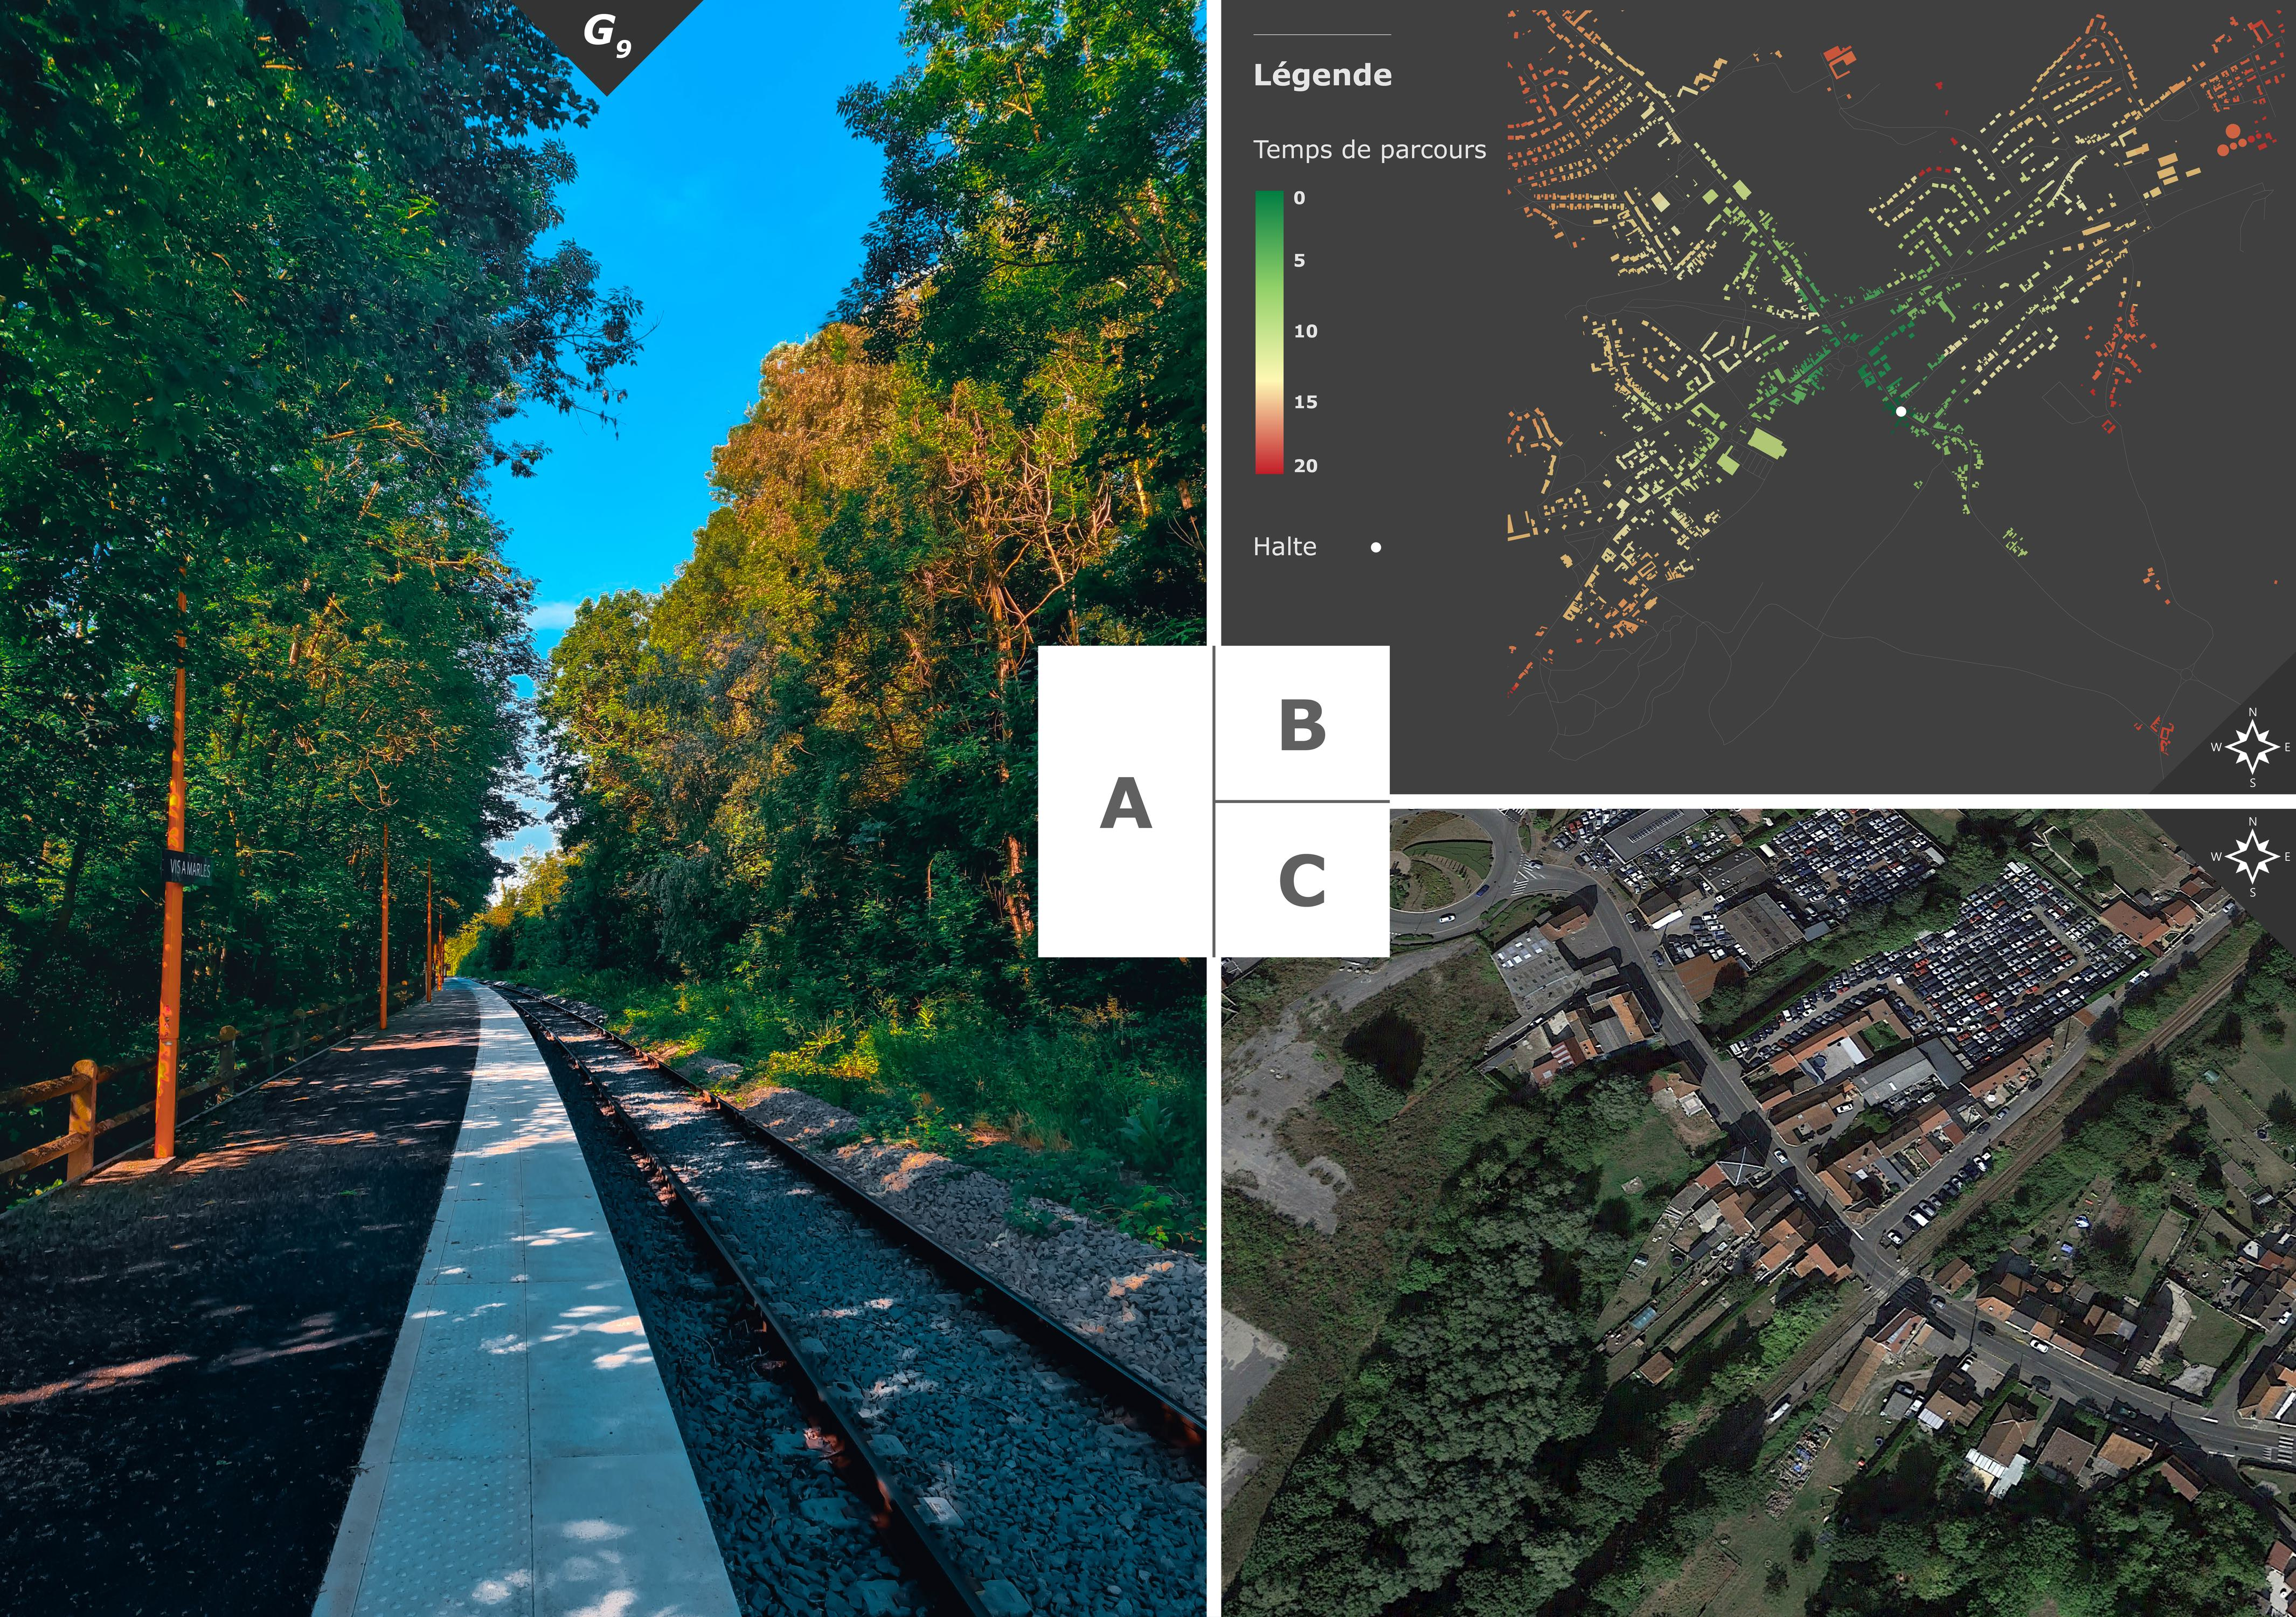
\includegraphics[height=.35\pageheight]{src/Figures/Chap-3/FR_Gare_VisaMarles.jpg}}
        \vspace{5pt}
        \begin{flushright}\scriptsize{
        Photographie (A)~: \textcolor{blue}{Dylan Moinse (2022)}
        \\
        Auteur (B)~: \textcolor{blue}{Dylan Moinse (2024)} avec les données issues d'\textcolor{blue}{\textcite{openstreetmap_openstreetmap_2023}}
        \\
      Jeux de données (C)~: données satellitaires issues de \textcolor{blue}{\textcite{google_earth_google_2023}}
      }\end{flushright}
      \end{carte}

    % Halte Vis-à-Marles (G9)
La halte de Vis-à-Marles (\(G_9\)) se différencie du corpus de gares étudiées par son rôle de desserte locale dans des territoires à faible et moyenne densité (voir la \hyperref[fig-chap3:monographie-vis-a-marles]{carte~\ref{fig-chap3:monographie-vis-a-marles}}, page~\pageref{fig-chap3:monographie-vis-a-marles}). En nous référant à la typologie des pôles d'échange multimodaux établie dans le \acrshort{SRADDET} de la \textcolor{blue}{\textcite[82]{region_hauts-de-france_sraddet_2024}}\index{Région Hauts-de-France@\textsl{Région Hauts-de-France}|pagebf}, il s'agit d'un \Guillemets{point d'arrêt}. Située à la périphérie de Marles-les-Mines, une commune résidentielle proche de Béthune, cette halte est reliée par une voie unique à la ligne \acrshort{TER} qui dessert Lille et Saint-Pol-sur-Ternoise via Béthune. Si celle-ci a accueilli 21~418 voyageur·se·s en 2023 \textcolor{blue}{\autocite{sncf_frequentation_2024}}\index{SNCF@\textsl{SNCF}|pagebf}, les usager·ère·s du transport public privilégient les trois lignes de bus qui s'arrêtent à proximité de la gare~: la ligne 30 desservant le centre-ville de Marles-les-Mines, la ligne 20 la connectant à Béthune et la ligne 68 atteignant la zone d'emploi de Bruay-la-Buissière. Cependant, l'absence de signalétique et de coordination claire entre les services de train et de bus rend le déplacement intermodal peu aisé. La proximité de la halte avec plusieurs communes ajoute une dimension intéressante pour les déplacements en train et en mobilité individuelle légère. Tandis que le centre urbain de Marles-les-Mines est situé à 1,5 kilomètre et celui de Lapugnoy à 2,5 kilomètres à pied, les communes plus peuplées comme Bruay-la-Buissière et Auchel, toutes deux situées à 4,1 kilomètres, sont potentiellement accessibles en cycle. Ces deux territoires dynamiques, dépourvus de système ferroviaire, pourraient bénéficier d'une connexion directe, à l'aide de cette synergie modale, à destination de Béthune et de Lille.%%Rédigé%%

    % Tableau Gares étudiées
% Gares étudiées
%%Rédigé%%
        \begin{table}[h!]
  \centering
  \renewcommand{\arraystretch}{1.5}
  \resizebox{\columnwidth}{!}{
  \begin{tabular}{p{0.2\columnwidth}p{0.48\columnwidth}p{0.15\columnwidth}p{0.17\columnwidth}}
    % \hline
    \rule{0pt}{15pt} \small{\textcolor{blue}{\textbf{Gare ou halte}}} & \small{\textcolor{blue}{\textbf{\acrshort{EPCI}}}} & \small{\textcolor{blue}{\textbf{Département}}} & \small{\textcolor{blue}{\textbf{Vélo* (2020)}}}\\
        \hline
    \multicolumn{4}{l}{\small{\textbf{Gare Lille Flandres} (\(G_1\))}}\\
\small{Lille} & \small{\acrfull{MEL}} & \small{Nord} & \small{6,6~\% (3,8~\%)}\\
        \hdashline
    \multicolumn{4}{l}{\small{\textbf{Gare de Dunkerque} (\(G_2\))}}\\
\small{Dunkerque} & \small{\acrfull{CUD}} & \small{Nord} & \small{3,5~\% (3,2~\%)}\\
        \hdashline
    \multicolumn{4}{l}{\small{\textbf{Gare de Béthune} (\(G_3\))}}\\
\multirow{1.5}{*}{\small{Béthune}} & \small{\acrfull{CABBALR}} & \multirow{1.5}{*}{\small{Pas-de-Calais}} & \multirow{1.5}{*}{\small{2,9~\% (1,4~\%)}}\\
        \hdashline
    \multicolumn{4}{l}{\small{\textbf{Gare d'Armentières} (\(G_4\))}}\\
\small{Armentières} & \small{\acrfull{MEL}} & \small{Nord} & \small{3,4~\% (3,8~\%)}\\
        \hdashline
    \multicolumn{4}{l}{\small{\textbf{Gare de Creil} (\(G_5\))}}\\
\small{Creil} & \small{\acrfull{ACSO}} & \small{Oise} & \small{1,1~\% (1,1~\%)}\\
        \hdashline
    \multicolumn{4}{l}{\small{\textbf{Halte Lille CHR} (\(G_6\))}}\\
\small{Lille} & \small{\acrfull{MEL}} & \small{Nord} & \small{6,6~\% (3,8~\%)}\\
        \hdashline
    \multicolumn{4}{l}{\small{\textbf{Gare de Lesquin} (\(G_7\))}}\\
\small{Lesquin} & \small{\acrfull{MEL}} & \small{Nord} & \small{2,2~\% (3,8~\%)}\\
        \hdashline
    \multicolumn{4}{l}{\small{\textbf{Halte Le Poirier Université} (\(G_8\))}}\\
\multirow{1.5}{*}{\small{Trith-Saint-Léger}} & \small{\acrfull{Porte du Hainaut}} & \multirow{1.5}{*}{\small{Nord}} & \multirow{1.5}{*}{\small{1,0~\% (1,8~\%)}}\\
        \hdashline
    \multicolumn{4}{l}{\small{\textbf{Halte Vis-à-Marles} (\(G_9\))}}\\
\multirow{1.5}{*}{\small{Marles-les-Mines}} & \small{\acrfull{CABBALR}} & \multirow{1.5}{*}{\small{Pas-de-Calais}} & \multirow{1.5}{*}{\small{0,9~\% (1,4~\%)}}\\
        \hline
        \end{tabular}}
    \caption{Répartition modale de l'usage monomodal du vélo dans les territoires d'implantation.}
    \label{table-chap3:part-modale-velo-gares-examinees}
        \vspace{5pt}
        \begin{flushleft}\scriptsize{
        \textcolor{blue}{Note~:} la dernière colonne du tableau se réfère à la part modale du vélo à l'échelle de la commune puis à celle de l'\acrshort{EPCI} entre parenthèses.
        \\
        \textcolor{blue}{Lecture~:} parmi les neuf gares examinées, les déplacements exclusifs à vélo sont bien plus développés à Lille, suivent la moyenne nationale à Dunkerque, à Armentières et à Béthune, et sont marginaux dans les communes de Lesquin, de Creil, de Trith-Saint-Léger et de Marles-les-Mines.
        }\end{flushleft}
        \begin{flushright}\scriptsize{
        Jeux de données liés à la part modale communale et intercommunale du vélo~: \textsl{Atlas vélo régional Hauts-de-France} de \textcolor{blue}{\textcite{velo__territoires_atlas_2023}}, elles-mêmes issues du fichier \textsl{Mobilités Professionnelles (MOBPro) du recensement de la population de 2020} de l'\textcolor{blue}{\textcite{insee_documentation_2023}}
        \\
        Jeux de données liés à l'offre de services vélo~: \textcolor{blue}{\textcite{sncf_voyageurs_stationnement_2023}}, \textcolor{blue}{\textcite{ilevia_abris_nodate}} et \textcolor{blue}{\textcite{openstreetmap_openstreetmap_2023}} 
        \\
        Auteur~: \textcolor{blue}{Dylan Moinse (2023)}
        }\end{flushright}
        \end{table}%%Rédigé%%

    % Transition
La description générale de la situation des neuf gares constituant la \Guillemets{scène} de notre enquête par observation directe, abordée sous les angles de la mobilité et des territoires, nous a permis d’obtenir une vue d’ensemble pour initier notre réflexion, en tant qu'entrée sur notre terrain de recherche. Cette première esquisse, élaborée à partir des gares étudiées, révèle l'importance que nous avons accordée à la diversité représentative des infrastructures ferroviaires présentes dans la région. La sélection des points nodaux inclut ainsi des pôles multimodaux structurants à différentes échelles géographiques, des gares stratégiques servant de portes d'entrée vers certaines agglomérations, des nœuds de rabattement à destination des zones d'emploi ainsi que des nœuds secondaires dotés d'un potentiel d'accès à certaines aménités territoriales. En parallèle de ces critères, nous avons également veillé à intégrer des territoires issus des anciennes régions et \acrshort{EPCI} composant les Hauts-de-France. Cette démarche permet de capturer une diversité de contextes territoriaux et de mettre en évidence les disparités en matière d’enjeux locaux, notamment en ce qui concerne le développement du vélo et des infrastructures cyclables (voir le \hyperref[table-chap3:part-modale-velo-gares-examinees]{tableau~\ref{table-chap3:part-modale-velo-gares-examinees}}, page~\pageref{table-chap3:part-modale-velo-gares-examinees}). Dans la section suivante du présent chapitre, nous allons exposer la méthodologie de notre questionnaire, conçu spécifiquement pour les voyageur·se·s intermodaux·les en mobilité individuelle légère. L’objectif de cet outil est de compléter les enseignements issus de l’observation quantitative, en offrant une perspective élargie et approfondie sur ces pratiques de mobilité.%%Rédigé%%

     % ___________________________________________
    % 3.4.
    \newpage
    \needspace{1\baselineskip} % Réserve de l'espace
    \sectionheader{Description du questionnaire}
\section{Enquête par questionnaire sur les pratiques intermodales
    \label{chap3:questionnaire}
    }

    % Intérêt du questionnaire croisé à l'observation
Le croisement d’une enquête par questionnaire avec des observations statiques s’inscrit dans un dispositif de recherche intégré, participant à améliorer la qualité de l'information recueillie. En combinant l’exploitation d’observations directes dans les lieux pratiqués avec le recueil de réponses individuelles au questionnaire, cette double approche permet de couvrir une diversité d’éléments, tels que les déplacements, les usages, les caractéristiques personnelles, les motivations, ainsi que les marquages sociaux induits \textcolor{blue}{\autocite[131]{dureau_lobservation_2014}}\index{Dureau, Françoise|pagebf}\index{Giroud, Matthieu|pagebf}\index{Lévy, Jean-Pierre|pagebf}. L’intérêt d’un tel système de collecte réside dans la capacité du questionnaire à saisir le \Guillemets{sens objectif des conduites}, dans un cadre préalablement défini, en confrontant ces renseignements mobilitaires avec des indicateurs relatifs aux déterminants sociaux et géographiques \textcolor{blue}{\autocite[68]{belfils_lepreuve_2002}}\index{Belfils, Aude|pagebf}. Ce niveau d’analyse jumelé~–~intégrant l'inventaire du \textsl{fait} et de \textsl{données déclaratives}~–~contribue à enrichir la compréhension des pratiques intermodale étudiées en adoptant une perspective à la fois analytique et compréhensive des dynamiques.%%Rédigé%%

    % Objectifs
L'objectif de notre questionnaire est double. Il s'agit d'approfondir la compréhension du phénomène \textsl{a priori} croissant de ces chaînages modaux et d'en examiner les déterminants socio-spatiaux. Grâce à un échantillonnage couvrant une variété de cas de figure et de territoires, tout en veillant à nous focaliser principalement sur les Hauts-de-France, le questionnaire vise à fournir une vision globale des pratiques de mobilité.%%Rédigé%%

    % Annonce du plan
Nous allons détailler le déploiement de notre enquête en ligne, en mettant en évidence ses apports stratégiques (voir la \hyperref[chap3:apports-questionnaire-usagers]{section sur les apports du questionnaire}, page~\pageref{chap3:apports-questionnaire-usagers}). Nous introduisons les avantages que représente la mise en place de cet outil en insistant sur sa plus-value par rapport aux limites des enquêtes de mobilité actuellement conduites en France, notamment en rapport avec notre objet d'étude. En lien avec notre positionnement scientifique, centré sur l'interaction entre les pratiques de mobilité et les agencements territoriaux, nous y présentons la manière dont le questionnaire est un cadre méthodologique justifié pour enrichir l'analyse ciblée sur les cyclo-voyageur·se·s. Nous décrivons ensuite son mode d'administration (voir la \hyperref[chap3:administration-questionnaire-usagers]{section sur le protocole du questionnaire}, page~\pageref{chap3:administration-questionnaire-usagers}) en abordant ses grands traits méthodologiques, ses modes de diffusion, sa structure générale au travers de l'organisation thématique et logique des questions, et le traitement des données statistiques et géographiques issues de l'échantillon construit.%%Rédigé%%

    % 3.4.1.
    \needspace{1\baselineskip} % Réserve de l'espace
\subsection{Apports du questionnaire
    \label{chap3:apports-questionnaire-usagers}
    }

    % Introduction
Les transformations rapides des pratiques de mobilité, caractérisées par l’essor de l’intermodalité et soutenues par l’émergence de nouvelles formes de mobilité individuelle légère, nous invitent à repenser les outils d’enquête. Les enquêtes publiques traditionnelles, conçues principalement pour couvrir de vastes territoires et répondre à des objectifs statistiques institutionnels, montrent des limites dans leur capacité à capter et à appréhender la diversité et la complexité des chaînes modales qui constituent l’objet de notre recherche. Le format et la fréquence des questionnaires tels que définis ne parviennent pas à offrir une vision à jour des pratiques de mobilité, se concentrant souvent sur des tendances globales de mobilité, au détriment des pratiques renouvelées. Le développement d’une approche complémentaire, mieux adaptée au paysage en mutation de la mobilité, s’est alors imposée dans notre cheminement méthodologique. Dans ce contexte, la création d’un formulaire spécifiquement conçu pour capturer ces pratiques de mobilité sous-représentées s’inscrit dans cette démarche. Dans cette sous-section, nous examinons comment un questionnaire sur-mesure est capable d'enrichir les connaissances à ce sujet et de répondre à ces défis qui s'alignent sur notre questionnement autour du \acrshort{TOD}.%%Rédigé%%

    % 3.4.1.1.
    \needspace{1\baselineskip} % Réserve de l'espace
\subsubsection*{Un formulaire dirigé vers des pratiques de mobilité sous-représentées dans les enquêtes publiques
    \label{chap3:apports-questionnaire-usagers-limites-enquetes-traditionnelles}
    }

    % Limites des enquêtes traditionnelles
Les enquêtes publiques nationales, telles que l'\acrfull{EMP}~–~prenant la suite de l'\acrfull{ENDT}~–~ainsi que les enquêtes régionales comme l'\acrfull{EMD} certifiée par le \acrshort{Cerema}, présentent certaines lacunes lorsqu’il s’agit de représenter des groupes sociaux spécifiques et émergents dans le paysage actuel de la mobilité. En particulier, ces enquêtes peinent à intégrer une perspective intermodale, indispensable pour appréhender les pratiques de mobilité combinant plusieurs modes de déplacement. Les questionnaires classiques conçus dans ces enquêtes à très large échelle sont souvent peu adaptés pour capturer la complexité et la diversité des chaînes de déplacement. Par ailleurs, un défi majeur réside dans le manque de contextualisation géographique des enquêtes métropolitaines. Celles-ci ont tendance à masquer l'étendue des bassins de mobilité, destinés à saisir l'ampleur des flux interurbains et les interactions territoriales. À titre d’exemple, l'\acrshort{EMD} de la \acrshort{MEL} n’inclut pas systématiquement les dynamiques de la deuxième couronne en direction du Bassin Minier. Comme le souligne \textcolor{blue}{Pascal} \textcolor{blue}{\textcite[29-30]{gabet_etude_2004}}\index{Gabet, Pascal|pagebf}, du fait de ces \Guillemets{découpages rigides}, cette omission limite la compréhension des interactions complexes entre les territoires et les flux interurbains qui les traversent. Ces lacunes méthodologiques appellent à une refonte des approches d’enquête, en intégrant des outils et des cadres d’analyse plus adaptés aux pratiques de mobilité émergentes et intermodales, tout en tenant compte des spécificités des territoires au-delà des découpages administratifs conventionnels.%%Rédigé%%

    % Un questionnaire sur-mesure pour combler les lacunes
Pour répondre à ces limites, nous avons cherché à développer un outil de collecte de données adapté aux réalités locales et aux comportements de mobilité émergents. La construction d'une \Guillemets{enquête sur-mesure}, de nature plus \Guillemets{artisanale} \textcolor{blue}{\autocite[42]{singly_questionnaire_2016}}\index{Singly, François de|pagebf}, s'impose comme une méthodologie complémentaire aux enquêtes institutionnelles standardisées. \textcolor{blue}{François de} \textcolor{blue}{\textcite[42]{singly_questionnaire_2016}}\index{Singly, François de|pagebf} qualifie cette approche de plus ciblée dès lors qu'elle permet de capturer des dynamiques sociales et individuelles souvent occultées par les \Guillemets{méthodes quantitatives lourdes}, bien documentées. Selon \textcolor{blue}{\textcite[8]{armoogum_rapport_2018}}\index{Armoogum, Jimmy|pagebf}\index{Tebar, Maria|pagebf}\index{Christian, Barbara|pagebf}\index{Garcia, Cédric|pagebf}\index{Nguyen, Minh-Hieu|pagebf}\index{Rendina, Fabio|pagebf}, les enquêtes sur papier ou par téléphone, où les participant·e·s doivent décrire leur comportement de mobilité sur une journée ou reconstituer des déplacements antérieurs, génèrent automatiquement des biais par rapport au comportement réel. De plus, leur coût élevé et leur faible fréquence réduisent leur capacité à capter les mutations rapides des pratiques sociales en mouvement. Ces enquêtes classiques offrent alors une vision plus statique et plus réductrice de la mobilité, fondée sur l'hypothèse que les déplacements réalisés lors d'un jour moyen de semaine sont reproductibles. Cette hypothèse a notamment été remise en cause puisqu'elle écarte les dynamiques contextuelles et les événements imprévisibles \textcolor{blue}{\autocite{madre_dynamiser_2004}}\index{Madre, Jean-Loup|pagebf}\index{Gascon, Marie-Odile|pagebf}.%%Rédigé%%

    % Une nouvelle approche centrée sur l'intermodalité
La conception d'un formulaire adapté aux pratiques de mobilité s'inscrivant dans une perspective intermodale repose sur plusieurs principes. Premièrement, une meilleure adaptation scalaire aux bassins de mobilité des cyclo-voyageur·se·s. Deuxièmement, une capture du chaînage modal en documentant les étapes successives et les connexions. Troisièmement, une adaptabilité par le biais de canaux de communication diversifiés, se matérialisant par des prises de contact \textsl{in situ} et en ligne, afin de réduire les biais d'échantillonnage. Quatrièmement et dans le prolongement avec les principes précédemment formulés, un recrutement s'appuyant principalement sur le mouvement en cours de réalisation, dans le but de limiter les biais de mémoire.%%Rédigé%%

    % 3.4.1.2.
    \needspace{1\baselineskip} % Réserve de l'espace
\subsubsection*{Plus-value du questionnaire
    \label{chap3:apports-questionnaire-usagers-plus-value}
    }

    % Nature du questionnaire
L’utilisation du questionnaire dans le cadre d’une recherche sur les pratiques intermodales présente de nombreux avantages, tant pour la caractérisation des comportements que pour leur compréhension et l’évaluation des politiques publiques. Cet outil méthodologique permet d’offrir une vision à la fois large et précise des pratiques de mobilité, tout en rendant possible une analyse fine des dynamiques comportementales, spatiales et politiques. Il s'agit d'un instrument pertinent pour identifier les freins et les leviers liés à l’usage intermodal de la mobilité individuelle légère. Il s’inscrit dans une démarche explicative \textcolor{blue}{\autocite[20]{singly_questionnaire_2016}}\index{Singly, François de|pagebf}, faisant appel à la \Guillemets{cognition automatique}\footnote{ 
    À l’interface entre sociologie explicative et sociologie compréhensive, \textcolor{blue}{Stephen} \textcolor{blue}{\textcite[1~683]{vaisey_motivation_2009}}\index{Vaisey, Stephen|pagebf} distingue deux types de cognition~: la \Guillemets{cognition réflexive} (\textsl{discursive cognition}), où les individus sont invités à justifier leurs actions, nécessitant des outils comme l’entretien approfondi, et la \Guillemets{cognition automatique} (\textsl{practical cognition}), qui se concentre sur des actions quasi spontanées ou routinières, pour lesquelles le questionnaire est particulièrement adapté. Le premier type de cognition correspond aux explications explicites que les individus donnent pour rationaliser ou justifier leurs actions ou croyances, celle-ci est consciente et réfléchie. Le seconde type de cognition concerne les schémas intériorisés qui orientent les individus vers certaines actions.
} \textcolor{blue}{\autocite[1~683]{vaisey_motivation_2009}}\index{Vaisey, Stephen|pagebf}.%%Rédigé%%

    % Liste avantages
Dans ce contexte, cinq principaux avantages justifient l’adoption de cette méthode en complément de l'observation quantitative~:
    \begin{customitemize}
\item \textsl{Révélation des déterminants comportementaux}~: le questionnaire permet de décrire les choix préférentiels des usager·ère·s tout en identifiant les raisons sous-jacentes à ces choix. En combinant des questions fermées avec des questions ouvertes ponctuelles, il devient possible d’enrichir la compréhension des mécanismes sous-jacents aux préférences modales et de mieux saisir la complexité des comportements observés \textcolor{blue}{\autocite[4, 9]{meissonnier_pour_2012}}\index{Meissonnier, Joël|pagebf}. La forme que prend le questionnaire permet ainsi de repérer les \Guillemets{schèmes de perception durablement incorporés} dans les comportements des cyclo-voyageur·se·s \textcolor{blue}{\autocite[1~680]{vaisey_motivation_2009}}\index{Vaisey, Stephen|pagebf}~;
\item \textsl{Exploration des relations entre espaces et pratiques}~: le questionnaire constitue un outil pertinent pour analyser le lien entre les caractéristiques des espaces traversés ou habités et les pratiques intermodales. Il prend en compte la diversité des stratégies de mobilité adoptées par les utilisateur·rice·s de la mobilité individuelle légère \textcolor{blue}{\autocite[2]{sebille_saisir_2024}}\index{Sebille, Pascal|pagebf}\index{Demoraes, Florent|pagebf}~;
\item \textsl{Profil des usager·ère·s}~: le questionnaire permet d'établir une segmentation fine des répondant·e·s, basée sur des critères socio-démographiques, géographiques ou comportementaux~;
\item \textsl{Standardisation et comparabilité des données}~: en recueillant des données statistiques standardisées, le questionnaire peut faciliter la comparabilité des résultats \textcolor{blue}{\autocite[5]{sebille_saisir_2024}}\index{Sebille, Pascal|pagebf}\index{Demoraes, Florent|pagebf}. À l'aide d'indicateurs homogénéisés,  il est possible de comparer différentes zones géographiques ou périodes~;
\item \textsl{Évaluation des politiques publiques}~: les données recueillies permettent d’évaluer l’impact perçu des aménagements et des mesures publiques sur les comportements de mobilité. Cette évaluation fournit des indices pour ajuster les politiques publiques en fonction des besoins et des attentes identifiés.
    \end{customitemize}%%Rédigé%%

    % 3.4.2.
    \needspace{1\baselineskip} % Réserve de l'espace
\subsection{Administration d'un questionnaire en ligne auprès des usager·ère·s en France
    \label{chap3:administration-questionnaire-usagers}
    }

    % Introduction
Conçu pour documenter les déplacements intermodaux combinant l’usage des transports en commun, du vélo et de la micro-mobilité, le questionnaire s’impose comme l’outil principal de collecte de données. En replaçant les données dans une perspective territoriale et comportementale, cette enquête contribue à enrichir les cadres d’analyse actuels des mobilités contemporaines. Il vise à étudier avec précision les chaînes de déplacement, en incorporant à la fois des dimensions quantitatives et qualitatives. Cette approche intégrée tient également compte des contextes géographiques dans lesquels s'inscrivent les pratiques de mobilité. Cette seconde sous-section détaille le processus d’exploitation de l'enquête numérique, depuis sa phase de conception jusqu'à la construction de l'échantillon et au traitement des données géostatistiques récoltées.%%Rédigé%%

    % 3.4.2.1.
    \needspace{1\baselineskip} % Réserve de l'espace
\subsubsection*{Exploitation du questionnaire
    \label{chap3:administration-questionnaire-usagers-exploitation}
    }

    % Protocole général
Le questionnaire d’enquête constitue l’instrument central de la collecte des données, conçu pour recueillir des informations quantitatives et qualitatives auprès d’un public cible. Il a été conçu pour explorer les pratiques intermodales impliquant la combinaison de modes de mobilité individuelle légère et de réseaux de transport en commun. La structure du questionnaire s’organise autour d’une description détaillée du dernier déplacement intermodal réalisé à l'aide d'un vélo ou d’une solution de micro-mobilité. Compte tenu de la faible représentation de la population cible à des échelles locales, sa diffusion a été étendue aux niveaux national et européen. Ce choix stratégique vise à garantir une couverture géographique large et à éviter les biais liés à une concentration excessive des répondant·e·s dans les agglomérations les plus denses.%%Rédigé%%

    % Support du questionnaire
Le questionnaire auto-administré, d’une durée estimée à quinze minutes, a été déployé sur la plate-forme \Marque{LimeSurvey}, un outil reconnu pour ses fonctionnalités avancées\footnote{
    \Marque{LimeSurvey} (\url{https://www.limesurvey.org/fr}) est un outil en libre accès en ligne, dédié à la création de questionnaires statistiques avancés \textcolor{blue}{\autocite{limesurvey_limesurvey_nodate}}\index{LimeSurvey@\textsl{LimeSurvey}|pagebf}.
}. Disponible en deux langues, français et anglais, le questionnaire en ligne a été accessible entre avril 2022 et janvier 2023. Le recours au format numérique répond à plusieurs objectifs stratégiques. Premièrement, il permet d’atteindre des populations cibles souvent difficiles à identifier sur le terrain, notamment dans les espaces de flux, au sein desquels les usager·ère·s ayant recours à un vélo à ou une option de micro-mobilité, ne sont pas toujours visibles, en particulier lorsque leurs véhicules sont stationnés. Deuxièmement, la version numérique offre des fonctionnalités puissantes pour concevoir un questionnaire détaillé et structuré, tout en garantissant une facilité d’exportation et d’analyse des données collectées. Enfin, le choix de \Marque{LimeSurvey} a été rendu possible par l’abonnement institutionnel souscrit par l’Université Gustave Eiffel, qui a permis un accès privilégié à l’ensemble des fonctionnalités offertes par cette plate-forme.%%Rédigé%%

    % Figure Affiche questionnaire (français)
    \begin{figure}[h!]\vspace*{4pt}
        \caption{Affiche du questionnaire auprès des usager·ère·s, en français.}
        \label{fig-chap3:affiche-questionnaire}
        \centerline{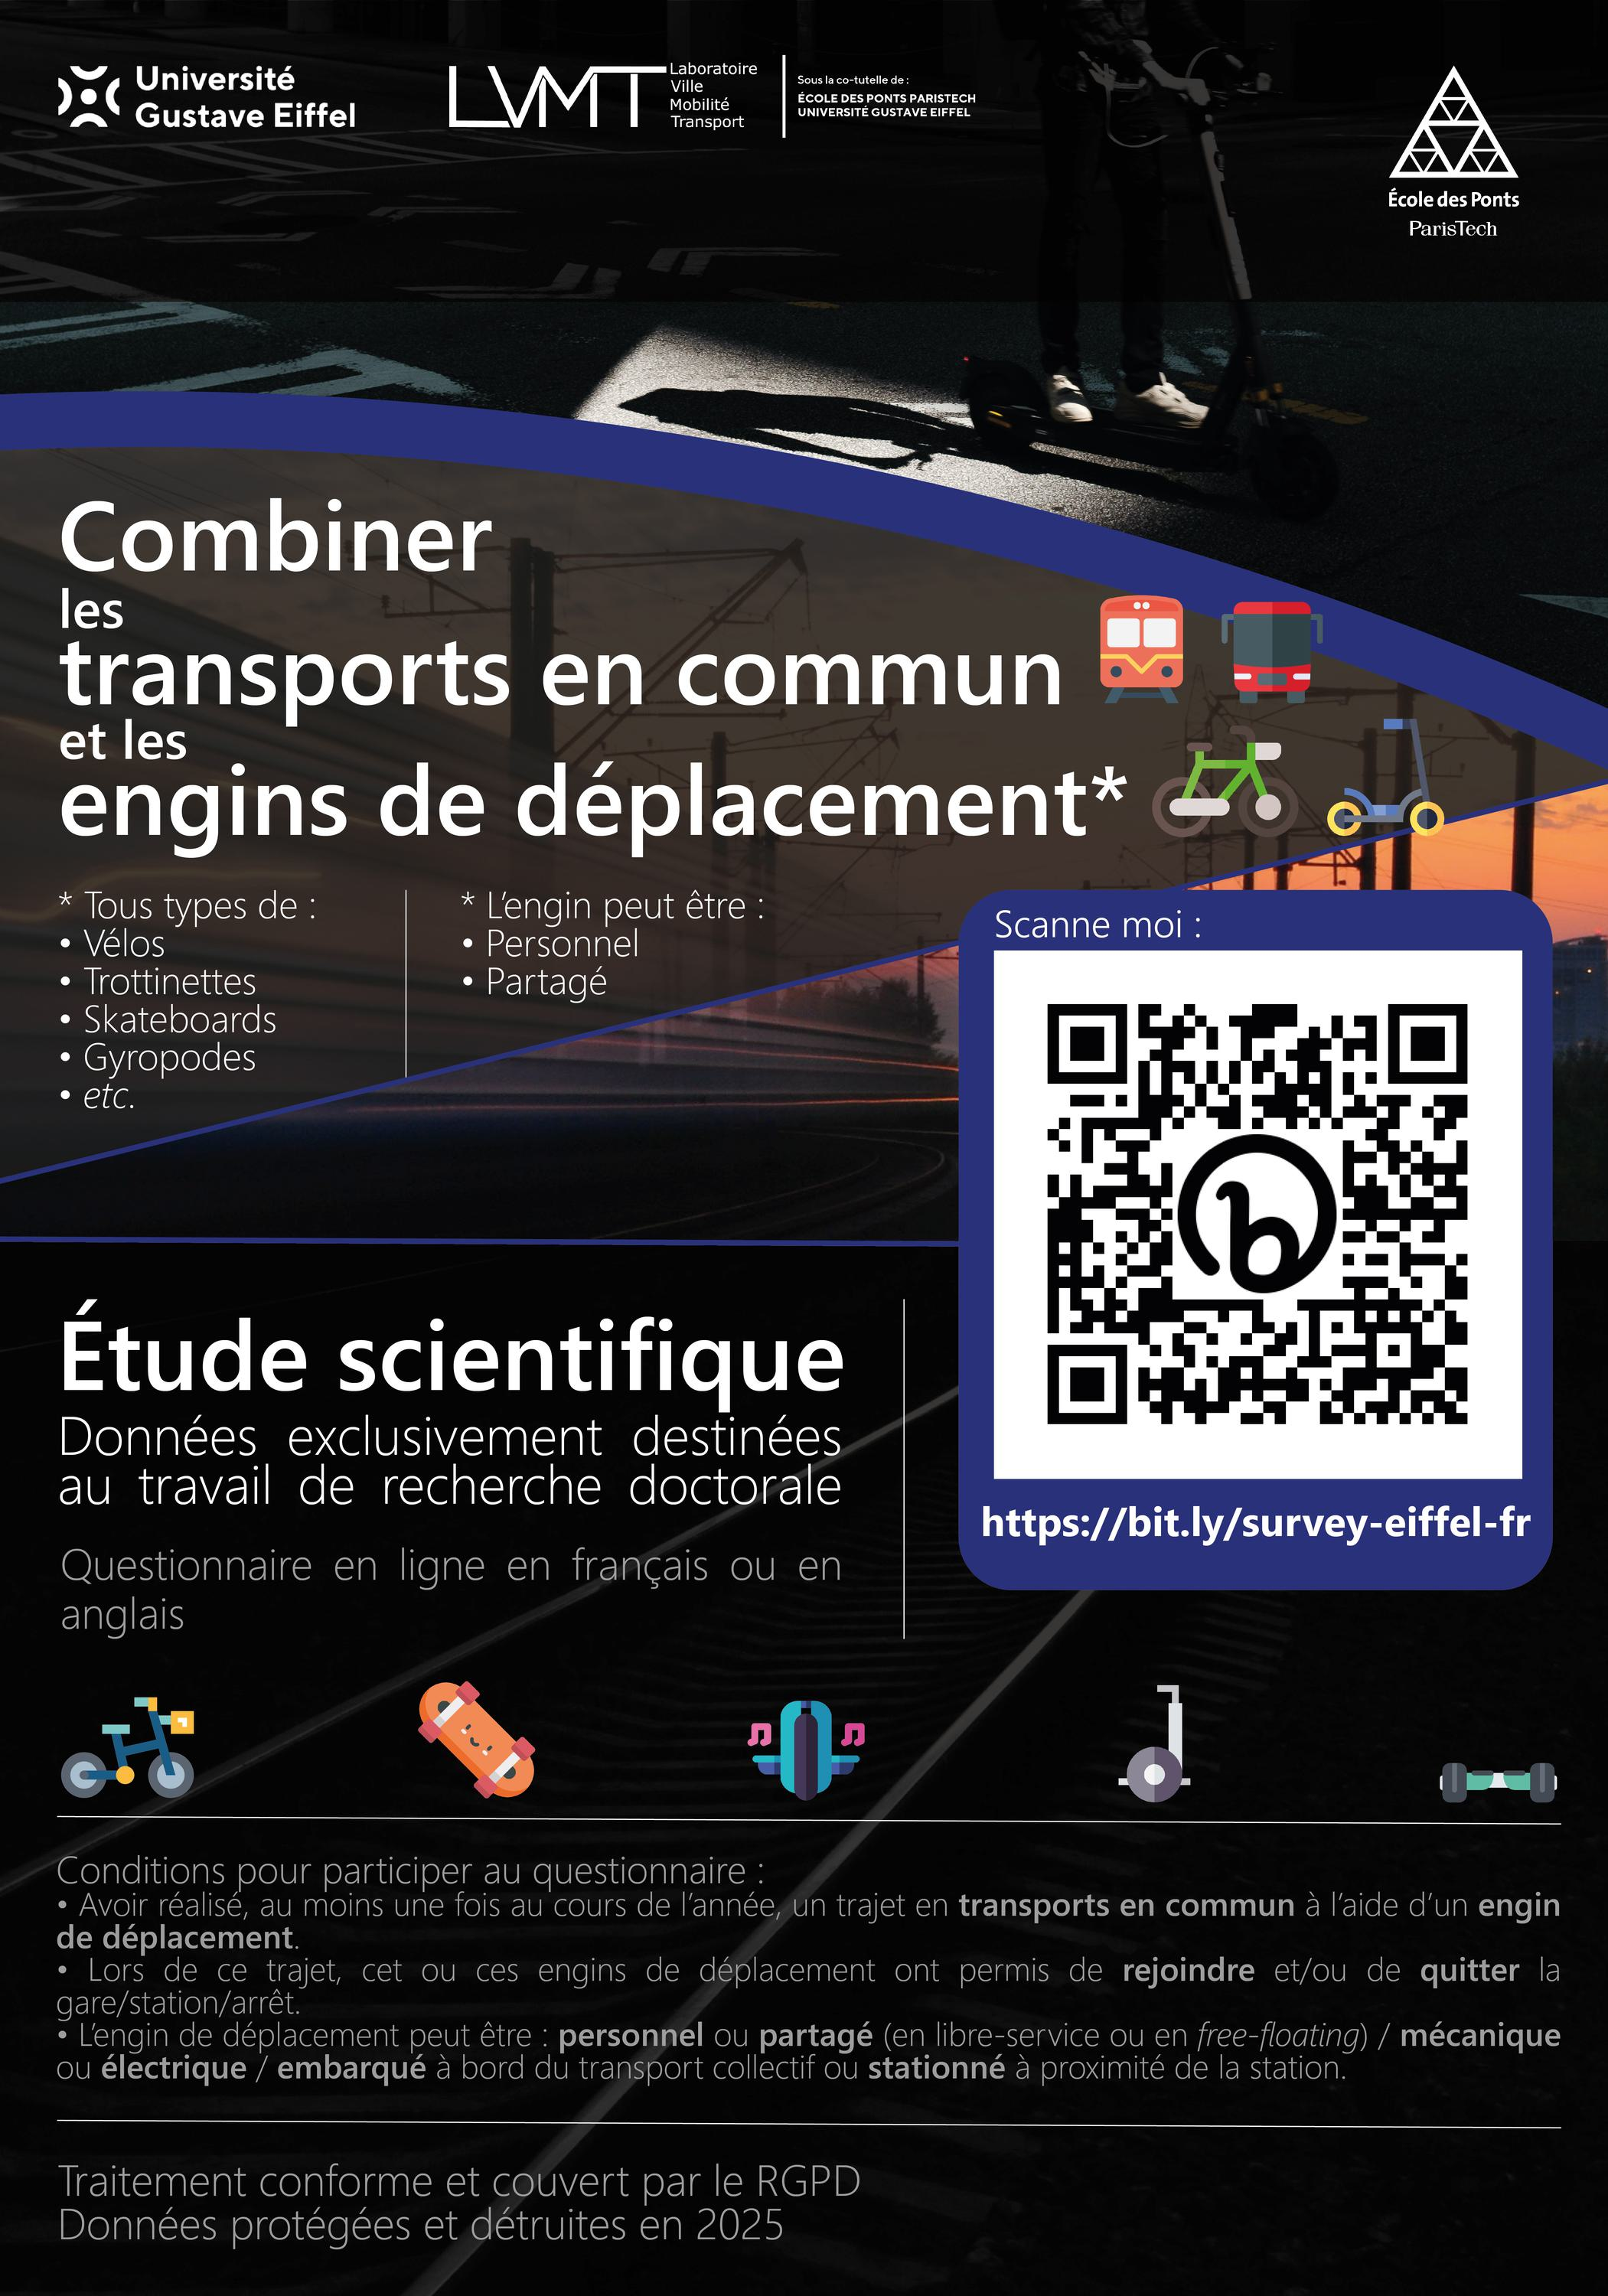
\includegraphics[width=1\columnwidth]{src/Figures/Chap-3/FR_Affiche_Questionnaire.jpg}}
        \vspace{5pt}
        \begin{flushright}\scriptsize{
        Auteur~: \textcolor{blue}{Dylan Moinse (2021)}
        }\end{flushright}
    \end{figure}

    % Campagnes de diffusion
Bien que la campagne de diffusion ait été menée à l’échelle nationale et internationale, une attention particulière a été portée sur la région Hauts-de-France, grâce à des stratégies de diffusion mises en œuvre~: 
\begin{customitemize}
    \item \textsl{Tractage en gare}. Des flyers ont été distribués sur les quais de neuf gares des Hauts-de-France\footnote{
        Au total, 864 flyers ont été distribués en main propre à des cyclo-voyageur·se·s~: 336 à la gare Lille Flandres, 177 pour Béthune, 109 à la halte Lille CHR, 84 pour Armentières, 70 pour Dunkerque, 49 pour Lesquin, 34 pour Creil, 5 à la halte du Poirier Université et 0 à la halte de Vis-à-Marles.
    }, après obtention de l’autorisation de \textsl{SNCF Gares \& Connexions}. Cette approche vise à toucher directement les usager·ère·s dans un environnement propice à l’identification des pratiques intermodales~;
    \item \textsl{Diffusion numérique, ciblée sur les réseaux sociaux et autres canaux régionaux}. Le questionnaire a été largement diffusé par voie électronique à travers des listes de diffusion académiques, associatives et professionnelles, ainsi que via les réseaux sociaux\footnote{
        Parmi les canaux mobilisés figurent les listes de diffusion scientifique en géographie, à la fois francophone (\textsl{Geotamtam}) et anglophone (\textsl{URB-GEOG-FORUM}), ainsi que les communications internes de l'Université Gustave Eiffel, telle la liste \textsl{info-événement-scientifique}. Nous avons également sollicité l'aide de l'association \acrfull{ADAV} au travers de son infolettre (environ 3~000 adhérent·e·s). Enfin, certains réseaux sociaux ont été utilisés, à l'instar de \textsl{X} (anciennement \textsl{Twitter}) ou \textsl{LinkedIn}. De plus, des groupes publics et privés au sein de \textsl{Facebook} ont servi de relai, incluant \textsl{Vélotaf} (52~300 membres), \textsl{Trottinette électrique~–~Rider's Français} (34~700 membres), \textsl{Vélo et train en France} (30~700 membres), \textsl{Les Usagers des TER Hauts-de-France} (11~200 membres) et \textsl{Cyclistes à Lille} (8~800 membres). D'autres \Guillemets{communautés} \textsl{Facebook} ont hébergé nos publications, mais leur contenu a été supprimé par la modération, souvent dans des espaces dédiés à la trottinette électrique.
    }. Des groupes spécifiques en lien avec le vélo, la micro-mobilité et les transports en commun ont été mobilisés pour maximiser l’engagement des publics concernés~;
    \item \textsl{Collage d'affiches}. Des affiches ont été apposées dans des lieux de passage tels que les campus de Villeneuve d’Ascq et de Champs-sur-Marne (voir l'\hyperref[annexes:affiche-en-questionnaire-usagers]{annexe~\ref{annexes:affiche-en-questionnaire-usagers}}, page~\pageref{annexes:affiche-en-questionnaire-usagers}).  
\end{customitemize}%%Rédigé%%

    % Critères de participation et RGPD
Pour participer à l'enquête, les participant·e·s devaient nécessairement avoir effectué, dans l'année précédant leur réponse, au moins un déplacement intermodal intégrant une forme de mobilité individuelle légère à un réseau de transport en commun. Ce critère d'éligibilité, permettant de cibler les voyageur·se·s intermodaux·les recherché·e·s dans cette étude, constitue la seule condition préalable pour répondre au questionnaire, peu importe la localisation géographique de l'itinéraire emprunté. Du point de vue des répondant·e·s, une garantie d’anonymisation et de protection des données personnelles a été assurée, conformément aux normes éthiques et légales en vigueur. L’enquête par questionnaire a été conçue et administrée, de façon responsable, dans le respect strict du \acrfull{RGPD}. À ce titre, les données collectées ont été systématiquement anonymisées afin de préserver la confidentialité des participant·e·s. Leur utilisation est strictement limitée au cadre de cette recherche, incluant une exploitation exclusive dans ce manuscrit ainsi que dans des publications et des communications scientifiques. Enfin, la durée de conservation des données a été plafonnée à cinq ans, conformément aux recommandations réglementaires.%%Rédigé%%

    % 3.4.2.2.
    \needspace{1\baselineskip} % Réserve de l'espace
\subsubsection*{Structure du questionnaire
    \label{chap3:administration-questionnaire-usagers-structure}
    }

    % Types de question
Le questionnaire se compose principalement de questions semi-fermées qui permettent de combiner des options de réponse prédéfinies avec des champs libres pour des réponses ouvertes. Cette conception inclut ainsi, de manière systématique, des choix de réponse tels que \Guillemets{\textsl{Je ne sais pas}}, \Guillemets{\textsl{Je ne veux pas y répondre}} et \Guillemets{\textsl{Autre}}, cette dernière option offrant aux répondant·e·s la possibilité de formuler une réponse textuelle. Ajoutons que nous avons veillé à intégrer, à chaque fin de section, une question générale et ouverte qui ne sert que si le sujet souhaite ajouter des remarques supplémentaires. L’ensemble des questions posées est obligatoire, à l’exception de ces dernières et de celles relatives au profilage des usager·ère·s, qui restent facultatives. Certaines questions sensibles, notamment celles concernant la localisation précise des étapes du déplacement, ont été rendues obligatoires malgré une réticence observée chez certain·e·s répondant·e·s. Ce choix, pleinement assumé, a pour but de garantir une qualité analytique et géographique optimale des données collectées. Par ailleurs, l’utilisation de l’outil \Marque{LimeSurvey} a permis d’intégrer un nombre intéressant de questions conditionnelles, personnalisant ainsi le parcours du questionnaire en fonction des réponses précédemment fournies. Cette flexibilité a rendu possible une meilleure prise en compte de la diversité des profils des cyclo-voyageur·se·s, tout en réduisant leur charge cognitive. Le questionnaire a effectivement été conçu pour être à la fois accessible et suffisamment détaillé afin de répondre aux objectifs de l’étude.%%Rédigé%%

    % Organisation thématique
Le questionnaire, que nous avons intitulé \Guillemets{Étude sur la combinaison du vélo et de la micro-mobilité avec les transports en commun}
(\textsl{Investigation into the Integration of Cycling and Micromobility with Public Transport}), s'articule autour de huit sections, précédées d'une brève introduction présentant le projet de recherche. Une description détaillée de cette organisation est fournie dans l'\hyperref[annexes:structure-questionnaire-usagers]{annexe~\ref{annexes:structure-questionnaire-usagers}} (page~\pageref{annexes:structure-questionnaire-usagers}).%%Rédigé%%

    % Liste sections
Les sections principales sont les suivantes~:
\begin{customitemize}
    \item \textsl{Introduction} (\(T_{0}\)). Présentation de l'étude, mise en conformité avec le \acrshort{RGPD} et coordonnées de l'enquêteur~; 
    \item \textsl{Consentement éclairé} (\(T_{1}\)). Recueil de l'accord formel des participant·e·s concernant le traitement de leurs données personnelles et sensibles~;
    \item \textsl{Organisation du déplacement intermodal} (\(T_{2}\)). Identification des étapes du chaînage modal, des noms des stations d'origine, de destination et de correspondance. Cette section inclut également des questions sur les types de mobilité individuelle légère utilisés, leur motorisation éventuelle, leur propriété, ainsi que sur la perception du confort des différents segments du déplacement~;
    \item \textsl{Localisation géographique des différents points d'arrêt} (\(T_{3}\)). Recueil des points de repère associés aux lieux d’origine et de destination, à l’aide d’adresses déclarées et de cartes interactives générées par \textsl{OpenStreetMap}, pour une précision géographique accrue. Des questions supplémentaires abordent la forme des itinéraires empruntés, à savoir notamment si le chemin emprunté est \Guillemets{le plus court}, afin de pallier l’absence de données de traçage \acrfull{GPS}~;
    \item \textsl{Modalités d'emport ou de stationnement} (\(T_{4}\)). Collecte des pratiques liées à l’embarquement ou au stationnement des véhicules personnels utilisés durant le déplacement~;
    \item \textsl{Caractéristiques du déplacement intermodal} (\(T_{5}\)). Recueil des informations sur la fréquence, les motifs, les motivations, l’expérience intermodale et les éventuels effets de substitution modale associés aux déplacements intermodaux~;
    \item \textsl{Habitudes de mobilité} (\(T_{6}\)). Analyse des pratiques de mobilité habituelles, incluant le rapport aux autres formes de mobilité, l’équipement des ménages (vélo, automobile, permis de conduire, abonnements, \textsl{etc.}) ainsi que les choix résidentiels~;
    \item \textsl{Profil socio-démographique} (\(T_{7}\)). Collecte facultative des informations générales sur les participant·e·s, telles que le genre, l’âge, le statut socio-professionnel, le niveau d’éducation, la composition du foyer, les revenus, \textsl{etc.}~;
    \item \textsl{Remerciements et recrutement} (\(T_{8}\)). Cette section facultative conclut le questionnaire par des remerciements aux participant·e·s et les invite à fournir des commentaires libres enrichissant l’enquête. Elle propose également de les rediriger vers une adresse courriel s’iels souhaitent recevoir les résultats de l’étude ou se porter volontaires pour un entretien sous forme de parcours commenté. Cette étape intermédiaire garantit le maintien de l’anonymat des réponses.
\end{customitemize}%%Rédigé%%

    % 3.4.2.3.
    \needspace{1\baselineskip} % Réserve de l'espace
\subsubsection*{Du \Guillemets{bon} échantillonnage~?
    \label{chap3:administration-questionnaire-usagers-echantillon}
    }

    % Représentativité
Dans son ouvrage méthodologique consacré à la conception des questionnaires en \acrfull{SHS}, \textcolor{blue}{François de} \textcolor{blue}{\textcite[38-42]{singly_questionnaire_2016}}\index{Singly, François de|pagebf} distingue quatre principales méthodes d’échantillonnage applicables une fois le public cible clairement défini~: l’échantillonnage statistique, la méthode des quotas, les échantillons stratifiés et l’étude des publics. Nous nous sommes orientés vers la dernière approche, à savoir l’échantillon probabiliste, qui consiste à sélectionner des individus de la population cible selon \Guillemets{les lois du hasard} \textcolor{blue}{\autocite[41]{singly_questionnaire_2016}}\index{Singly, François de|pagebf}. Cette méthode est spécifiquement adaptée à l'étude d'une population cible caractérisée par des groupes sociaux mobiles aux frontières diffuses. L’échantillon ainsi obtenu repose sur la spontanéité des répondant·e·s volontaires, ce qui en fait un échantillon non représentatif au sens strictement statistique. Cependant, comme le souligne \textcolor{blue}{Aude} \textcolor{blue}{\textcite[69]{belfils_lepreuve_2002}}\index{Belfils, Aude|pagebf}, l’objectif principal d’un tel échantillon est de fournir \Guillemets{une bonne représentation, une image stylisée par l’accentuation des traits pertinents}, dans l'optique de faire apparaître certaines dynamiques saillantes. La constitution d'un échantillon aléatoire, de nature non-probabiliste, repose ainsi sur une démarche scientifique qui ne prétend plus parler d'échantillon représentatif, mais dont l'objectif est de tendre vers un échantillon le plus représentatif possible.%%Rédigé%%

    % Processus de nettoyage
Au total, l'enquête a permis de recueillir 2~189 réponses, incluant à la fois des réponses partielles et complètes. Un processus de nettoyage des données a été mis en œuvre afin de ne conserver que les réponses suivant les critères attendus (voir le \hyperref[fig-chap3:echantillonnage-questionnaire]{schéma~\ref{fig-chap3:echantillonnage-questionnaire}}, page~\pageref{fig-chap3:echantillonnage-questionnaire}). Étant donné que les deux dernières sections, consacrées au profilage (\(T_{7}\)) et aux remerciements (\(T_{8}\)) sont optionnelles, une réponse est considérée comme complète lorsque les sept premières thématiques ont été intégralement renseignées.%%Rédigé%%

    % Figure Schéma nettoyage des données du questionnaire
    \begin{figure}[h!]\vspace*{4pt}
        \caption{Processus de nettoyage des réponses issues du questionnaire.}
        \label{fig-chap3:echantillonnage-questionnaire}
        \centerline{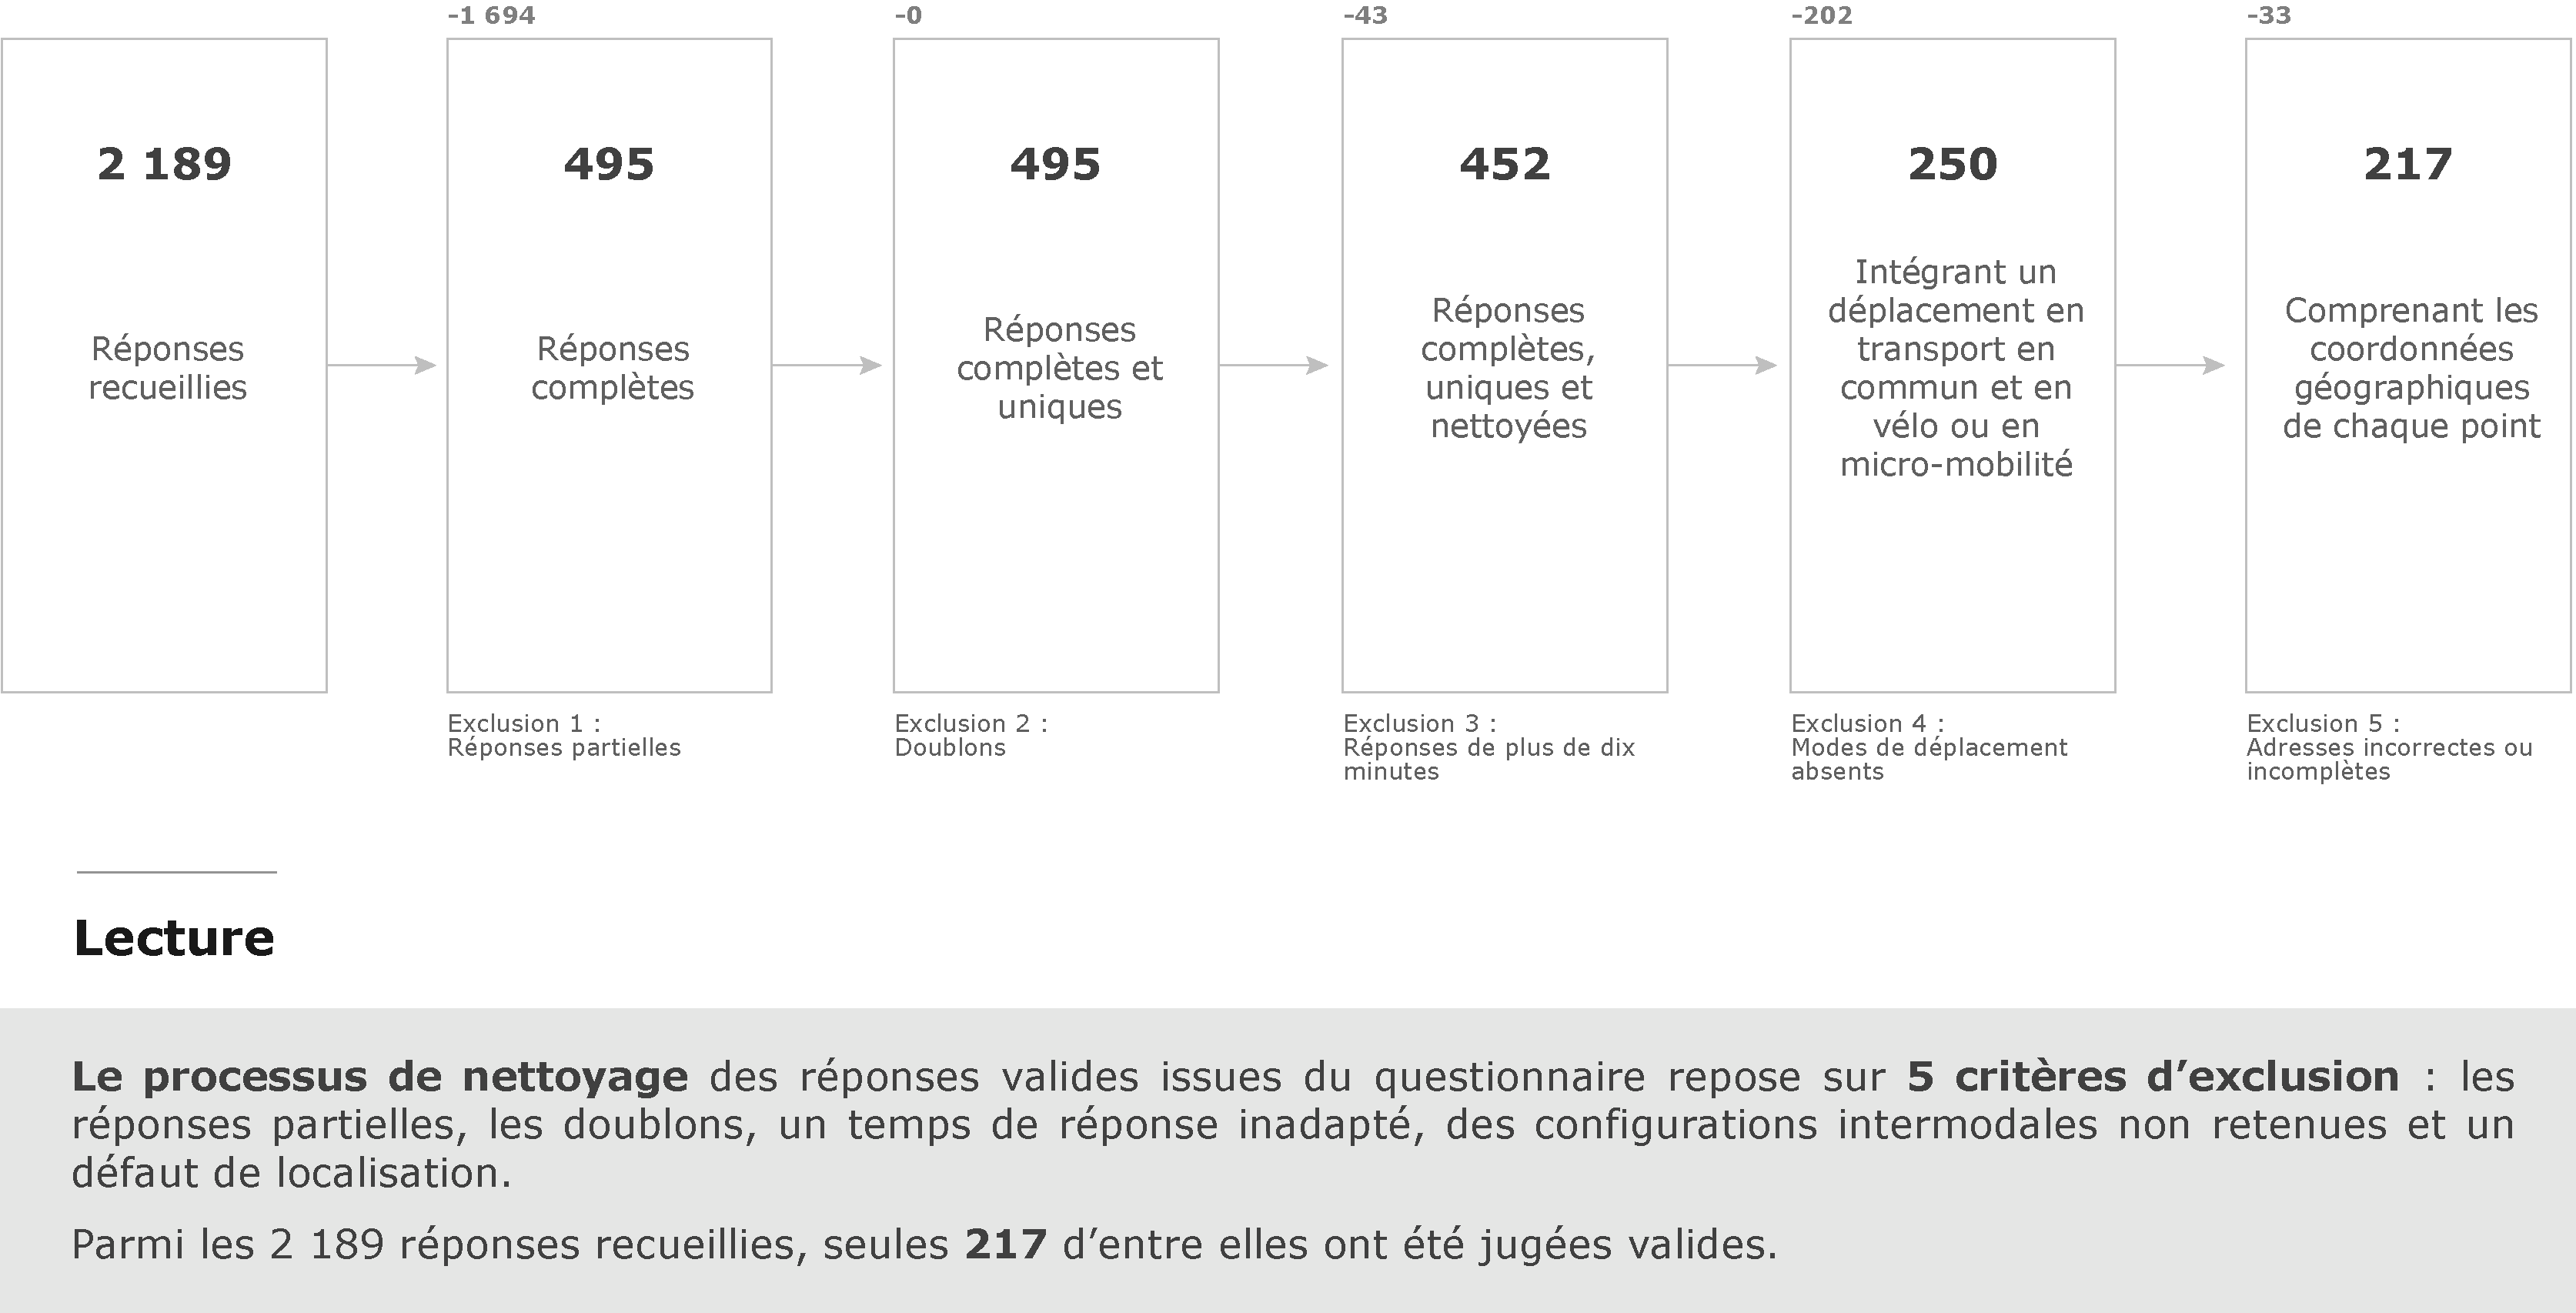
\includegraphics[width=1\columnwidth]{src/Figures/Chap-3/FR_Echantillon_questionnaire.pdf}}
        \vspace{5pt}
        \begin{flushright}\scriptsize{
        Auteur~: \textcolor{blue}{Dylan Moinse (2022)}
        }\end{flushright}
    \end{figure}

    % Nettoyage : exclusion 1 (partielles)
\textsl{Premier critère d'exclusion~: réponses partielles}. La première étape de ce processus a donc consisté à imputer les réponses partielles \textcolor{blue}{\autocite[12-13]{armoogum_rapport_2018}}\index{Armoogum, Jimmy|pagebf}\index{Tebar, Maria|pagebf}\index{Christian, Barbara|pagebf}\index{Garcia, Cédric|pagebf}\index{Nguyen, Minh-Hieu|pagebf}\index{Rendina, Fabio|pagebf}, ce qui a permis de retenir 495 réponses complètes. Comme anticipé, une proportion importante des réponses partielles s’interrompt au niveau de la section sensible dédiée à la spatialisation des déplacements intermodaux (\(T_{3}\)). Parmi les 1~694 réponses incomplètes (77,39~\%), 748 s’arrêtent précisément à cette étape, représentant 44,15~\% des réponses partielles. Une autre section critique peut être identifiée, puisque 244 réponses (14,40~\%) s’interrompent au niveau de la section relative aux habitudes de mobilité et aux aspirations résidentielles (\(T_{6}\)). Cette situation semble pouvoir s’expliquer, d’une part, par une charge cognitive jugée trop élevée en fin de questionnaire et, d’autre part, par une thématique perçue comme déconnectée des attentes des répondant·e·s, selon les retours recueillis dans les suggestions libres.%%Rédigé%%

    % Nettoyage : exclusion 2 (adresses IP)
\textsl{Deuxième critère d'exclusion~: doublons}. Bien que 495 réponses aient été initialement jugées complètes, des critères d'exclusion supplémentaires ont été appliqués pour garantir la qualité des données. Parmi ces critères figure l'exclusion des réponses dupliquées, identifiées lorsque deux ou plusieurs soumissions partagent une même adresse IP et présentent, dans le même temps, des réponses identiques. Cependant, après vérification, aucune saisie des données du questionnaire ne répond à ce critère d'exclusion.%%Rédigé%%

    % Nettoyage : exclusion 3 (temps de réponse)
\textsl{Troisième critère d'exclusion~: temps de réponse inadapté pour le questionnaire}. Un troisième critère d’exclusion a été appliqué, dans le but de maximiser la fiabilité des retours récoltés. Les soumissions ayant un temps de réponse inférieur à dix minutes ont été exclues, car ce délai a été jugé insuffisant pour compléter le questionnaire de manière réfléchie. Suite à cette étape, l’échantillon final a été réduit à 452 réponses, entraînant la mise à l'écart de 43 réponses complètes (8,69~\%). À titre informatif, le temps moyen relevé pour répondre au questionnaire s'élève à 17 minutes.%%Rédigé%%

    % Nettoyage : exclusion 4 (intermodalité)
\textsl{Quatrième critère d'exclusion~: configuration intermodale non retenue}. Ce critère, à fort impact, est lié au non-respect de la condition d’éligibilité au questionnaire, selon laquelle le déplacement décrit doit obligatoirement combiner un mode de mobilité individuelle légère avec un transport en commun. Malgré cette consigne, une proportion conséquente de réponses apportées portent sur des déplacements ne répondant pas à cette définition~: généralement, elles décrivent soit un déplacement exclusivement réalisé à vélo ou en micro-mobilité, soit un déplacement monomodal, consistant à alterner l'usage des transports en commun ou de la mobilité individuelle légère. Cette confusion, corroborée par les retours dans les commentaires libres, illustre la difficulté à aborder de manière explicite la notion d’intermodalité auprès des usager·ère·s, à travers un support dématérialisé\footnote{
    Dans sa thèse de doctorat sur la \Guillemets{structuration d'un méta-réseau intégré}, \textcolor{blue}{Pierre} \textcolor{blue}{\textcite[41]{ageron_intermodalite-voyageurs_2013}}\index{Ageron, Pierre|pagebf}\index{Varlet, Jean|pagebf} confirme la confusion entre plurimodalité et intermodalité.
}. En conséquence, 202 réponses ont été exclues sur cette base, représentant 44,69~\% de l’échantillon retenu après l’application des trois premiers critères d’exclusion. L’échantillon se compose alors de 250 réponses complètes.%%Rédigé%%

    % Nettoyage : exclusion 5 (adresses)
\textsl{Cinquième critère d'exclusion~: défaut de localisation d'un ou de plusieurs points de repère}. Le dernier critère d’exclusion appliqué concerne la géospatialisation des déplacements intermodaux. Pour chaque réponse, il était demandé que les points de repère des déplacements, qu’ils soient fournis sous forme d’adresses déclarées ou positionnés via la carte interactive, soient correctement référencés et cohérents. Lorsque des anomalies ou des incompatibilités ont été détectées, telles que des adresses mal déclarées ou des points de localisation géographique peu réalistes, les réponses correspondantes ont été exclues. Cette étape a conduit à l’élimination de 33 réponses (13,20~\%). À l’issue de l’application des cinq critères d’exclusion, l’échantillon final se compose de 217 réponses complètes et pleinement exploitables. Ces réponses décrivent des déplacements intermodaux valides et géoréférencés.%%Rédigé%%

    % Description de l'échantillon
L’échantillon final, composé de 217 réponses complètes et valides, présente une concentration géographique dans les régions Hauts-de-France (54,84~\%) et Île-de-France (18,43~\%). En revanche, seules 7 réponses proviennent de répondant·e·s situés en dehors de la France. Concernant les canaux de participation, 65 réponses valides (29,95~\%) ont été recueillies grâce à l'accès à un QR code disponible sur les flyers et les affiches, tandis que les 152 autres participant·e·s (70,05~\%) ont accédé au questionnaire en ligne par le biais des plate-formes numériques. Du point de vue des caractéristiques socio-démographiques des répondant·e·s, 41,47~\% des participant·e·s s’identifient comme femmes. Cette proportion est de loin supérieure à l'échantillon que nous avons pu collecter en gare (28,21~\%), grâce à l'observation quantitative. Mais cette part, tout comme les autres variables socio-démographiques de l'échantillon, se rapprochent des données issues d’enquêtes nationales sur les usager·ère·s des transports publics en France  \textcolor{blue}{\autocite[]{enov_enquete_2021}}\index{Enov@\textsl{Enov}|pagebf}.%%Rédigé%%

    % 3.4.2.4.
    \needspace{1\baselineskip} % Réserve de l'espace
\subsubsection*{Contrôle des données du questionnaire
    \label{chap3:administration-questionnaire-usagers-validation}
    }

    % Codage
L’analyse des données issues du questionnaire repose sur une structure préétablie visant à traduire le langage naturel des répondant·e·s en un langage numérique exploitable (\textcolor{blue}{Olivier} \textcolor{blue}{\textcite[49-62]{martin_analyse_2020}}\index{Martin, Olivier|pagebf}, cité par \textcolor{blue}{François de} \textcolor{blue}{\textcite[89]{singly_questionnaire_2016}}\index{Singly, François de|pagebf}). Cette étape de codage aboutit à la production du fichier informatique de l’enquête en attribuant un code pour chacune des réponses apportées, afin d’en faciliter le traitement et l’analyse ultérieurs. Le processus de codage peut intervenir au cours de différentes phases d'exploitation du questionnaire~: avant la saisie des données, pendant celle-ci ou bien après, comme l'explique l' \textcolor{blue}{\textcite{ined_saisie_nodate}}\index{Ined@\textsl{Ined}|pagebf}. Une partie des codes a ainsi été ajustée \textsl{a posteriori}, une fois l’intégralité des réponses aux questions ouvertes collectée. Ces réponses textuelles ont en effet nécessité un travail préalable de mise en inventaire, d’harmonisation et de regroupement thématique. Cette approche itérative a dès lors permis de générer un codage complémentaire adapté, spécifiquement destiné à l’analyse quantitative du questionnaire \textcolor{blue}{\autocite[89]{singly_questionnaire_2016}}\index{Singly, François de|pagebf}.%%Rédigé%%

    % Choix du plus court itinéraire
Dans une perspective géographique, nous avons cherché à projeter les itinéraires estimés des 217 déplacements intermodaux valides en nous appuyant sur leurs distances spatiales et temporelles. Cette démarche s’appuie sur le fait que 84~\% des répondant·e·s ont déclaré avoir \Guillemets{\textsl{utilisé le chemin le plus court pour se rendre ou sortir de la station de transport en commun}} (question \(Q_{03}^{T_{3}}*\)). En supposant alors que plus de quatre répondant·e·s sur cinq privilégient un accès direct et avec un minimum de détours aux différents nœuds du réseau et aux destinations visées, nous inscrivons notre analyse spatiale dans les travaux de \textcolor{blue}{\textcite[2, 7]{qiu_understanding_2022}}\index{Qiu, Xinze|pagebf}\index{Gao, Tianli|pagebf}\index{Yang, Yu|pagebf}\index{Luo, Ankang|pagebf}\index{Shang, Fan|pagebf}\index{Li, Ruiqi|pagebf} qui ont démontré l'adoption d'un tel comportement chez les cyclistes à Biejing, Shanghai et Xiamen, notamment en heures de pointe. Cette approche s’aligne également sur la réflexion de \textcolor{blue}{Frédéric} \textcolor{blue}{\textcite[115]{heran_distances_2009}}\index{Héran, Frédéric|pagebf}, qui établit que les piéton·ne·s et les cyclistes, mettant à contribution leur force physique, autrement dit un effort musculaire, sont particulièrement sensibles aux détours et tendent à adopter l’itinéraire le plus direct. Ce comportement relève plus largement du \Guillemets{principe du moindre effort} (\textsl{principle of least effort}) défini par le linguiste et philologue étasunien \textcolor{blue}{George Kingsley} \textcolor{blue}{\textcite[348]{zipf_human_1949}}\index{Zipf, George Kingsley|pagebf}, un concept centré sur la recherche de la minimisation des coûts imputables aux efforts physiques et cognitifs, auxquels peut participer le mouvement \textcolor{blue}{\autocite[348]{zhu_principle_2018}}\index{Zhu, Yueying|pagebf}\index{Zhang, Benwei|pagebf}\index{Wang, Qiuping~A.|pagebf}\index{Li, Wei|pagebf}\index{Cai, Xu|pagebf}.%%Rédigé%%

    % Projection des chemins les plus courts
En tenant compte de ces éléments, nous avons projeté les itinéraires en privilégiant la route la plus directe, dans la mesure où les voies empruntées sont accessibles au mode de déplacement déclaré pour chaque segment. Par exemple, les autoroutes ont été signalées comme étant accessibles pour les répondant·e·s se déplaçant en voiture lors des phases de rabattement ou de diffusion, mais exclues pour les modes à pied ou en mobilité individuelle légère. Dans le souci de surmonter la limitation due à l'absence de flux \acrshort{GPS}, souvent difficilement disponibles pour les modes personnels, nous avons basé notre analyse sur les coordonnées géographiques validées des lieux d’origine et de destination et des stations traversées. Les itinéraires ont été tracés à l’aide de la bibliothèque et l’outil de calcul d'itinéraires (\textsl{routing}) en ligne \Marque{GraphHopper}\footnote{
    \Marque{GraphHopper 0.13} (\url{https://www.graphhopper.com/}) est une plate-forme de planification d'itinéraires en source ouverte, lancée en 2019, et permettant le calcul des itinéraires routiers et en transport en commun, à partir des données d’\textsl{OpenStreetMap}, de la \textsl{Shuttle Radar Topography Mission} et des données \acrshort{GTFS} accessibles publiquement \textcolor{blue}{\autocite{graphhopper_graphhopper_2017}}. Grâce à sa performance élevée, le moteur est principalement utilisé par des applications de navigation et logistiques, mais également dans le cadre d'études sur l'accessibilité.
}, via l’interface cartographique \textsl{GraphHopper Maps} \textcolor{blue}{\autocite{graphhopper_graphhopper_2017}}\index{GraphHopper@\textsl{GraphHopper}|pagebf}. L'étape de géocodage nous a permis d’exporter les itinéraires sous format de sortie en \acrfull{GPX}\footnote{
    Un fichier \acrfull{GPX} contient principalement les points d'intersection (\textsl{waypoints}), les traces (\textsl{way}) et certaines données statistiques, comme la distance spatiale et temporelle, l'altitude ou encore les instructions de navigation. Ce type de format peut être exploité dans les logiciels \acrshort{SIG} ou dans les applications \acrshort{GPS}.
} et d’estimer plusieurs indicateurs clés, notamment les distances spatiales et temporelles ainsi que les niveaux de pente pour chaque tronçon. Par exemple, pour les 178 trajets effectués à vélo et en micro-mobilité et recensés parmi les 217 déplacements intermodaux, nous avons utilisé l’option \Guillemets{vélo utilitaire}, paramétrée avec une vitesse de déplacement moyenne de 16 kilomètres par heure \textcolor{blue}{\autocite[18]{sebban_complementarite_2003}}\index{Sebban, Annie-Claude|pagebf}.%%Rédigé%%

    % Transition
Après avoir présenté la méthodologie mise en œuvre pour concevoir le questionnaire destiné à collecter des données sur les déplacements intermodaux combinant mobilité individuelle légère et transport public, il apparaît pertinent de compléter cette démarche par des entretiens approfondis réalisés sur des échantillons de taille réduite. L'association méthodologique du questionnaire et de l'entretien constitue un apport riche à la compréhension fine de ces pratiques de mobilité, comme ont pu l'expérimenter \textcolor{blue}{\textcite[97]{dureau_lobservation_2014}}\index{Dureau, Françoise|pagebf}\index{Giroud, Matthieu|pagebf}\index{Lévy, Jean-Pierre|pagebf}. Dans cette perspective, la méthode des parcours commentés se révèle vivement intéressante puisqu'elle permet de saisir la complexité de ces pratiques. Elle constitue un outil complémentaire qui permet de recueillir des données qualitatives et \Guillemets{micro-géographiques} directement contextualisées \textcolor{blue}{\autocite[109]{bergeron_uncovering_2014}}\index{Bergeron, Julie|pagebf}\index{Paquette, Sylvain|pagebf}\index{Poullaouec-Gonidec, Philippe|pagebf}.%%Rédigé%%

     % ___________________________________________
    % 3.5.
    \newpage
    \needspace{1\baselineskip} % Réserve de l'espace
    \sectionheader{Description des parcours commentés}
\section{Enquête par entretien \textsl{in situ} sur les pratiques intermodales
    \label{chap3:parcours-commente}
    }

    % Introduction 1
Depuis le début des années 2000, les méthodes d’investigation scientifique mobilisées au sein des \acrfull{SHS} ont été profondément renouvelées par un changement de paradigme, identifié par \textcolor{blue}{\textcite[207]{sheller_new_2006}}\index{Sheller, Mimi|pagebf}\index{Urry, John|pagebf} et par \textcolor{blue}{\textcite{bonnet_territoires_2000}}\index{Bonnet, Michel|pagebf}\index{Desjeux, Dominique|pagebf} comme le \Guillemets{tournant de la mobilité} (\textit{Mobility Turn}). Ce tournant marque un retour en force des questions relatives aux mobilités dans le champ des sciences sociales, en distinguant l’étude du \textit{mouvement} de celle de la \textit{mobilité}. Face aux critiques formulées à l’encontre des approches de recherche qualifiées de \Guillemets{sédentaires}, ces nouvelles perspectives méthodologiques aspirent à devenir elles-mêmes aussi mobiles que les phénomènes qu’elles étudient \textcolor{blue}{\autocite[207]{buscher_mobile_2009}}\index{Büscher, Monika|pagebf}\index{Urry, John|pagebf}.%%Rédigé%%

    % Introduction 2
Cette dynamique engage une compréhension des déplacements quotidiens comme des pratiques construites et évolutives, ancrées dans les trajectoires de vie, façonnées par un champ des possibles, par ce qui est accessible et par les aspirations individuelles \textcolor{blue}{\autocite[40]{kaufmann_retour_2014}}\index{Kaufmann, Vincent|pagebf}. Dans ce cadre, des auteur·rice·s tel·le·s que \textcolor{blue}{Marie-Hélène} \textcolor{blue}{\textcite{massot_mobilites_2010}}\index{Massot, Marie-Hélène|pagebf} insistent sur l’urgence de concevoir des méthodes d’enquête véritablement \Guillemets{mobiles}, capables de dépasser les limites des approches \Guillemets{sédentaires}\footnote{
    Les méthodes dites \Guillemets{sédentaires}, caractéristiques des recherches traditionnelles sur les transports, qu’elles soient quantitatives ou qualitatives, sont souvent critiquées pour leur inadéquation face à la complexité inhérente aux mobilités contemporaines et à leurs multiples dimensions \textcolor{blue}{\autocites[110-111]{buscher_mobile_2009}[178]{merriman_rethinking_2014}}\index{Merriman, Peter|pagebf}\index{Büscher, Monika|pagebf}\index{Urry, John|pagebf}. Ces approches sédentaires peinent notamment à appréhender les expériences sensibles et émotionnelles liées aux mobilités, nécessitant de la part des participants un effort rétrospectif et une mise en mots souvent décontextualisée \textcolor{blue}{\autocite[107]{buscher_mobile_2009}}\index{Büscher, Monika|pagebf}\index{Urry, John|pagebf}.
}. En effet, tout déplacement engage le sujet dans une relation dynamique avec un environnement qui constitue une altérité \textcolor{blue}{\autocite[4]{despres_replacer_2019}}\index{Desprès, Michel|pagebf}\index{Lord, Sébastien|pagebf}\index{Negron-Poblete, Paula|pagebf}. Cette interaction, structurée par diverses médiations \textcolor{blue}{\autocite[]{freitag_dialectique_nodate}}\index{Freitag, Michel|pagebf}, peut se manifester sous la forme de stimuli sensoriels (\Guillemets{sensorimoteurs}), par le biais du langage (\Guillemets{symboliques}) ou encore par une interprétation des symboles (\Guillemets{formalisée}).%%Rédigé%%

    % Introduction 3
La compréhension de la complexité de la réalité sociale dépeinte doit passer par une transition des méthodes statiques vers des approches dynamiques \textcolor{blue}{\textcite[207]{sheller_new_2006}}\index{Sheller, Mimi|pagebf}\index{Urry, John|pagebf}. Dans cette perspective, il devient impératif de développer des techniques innovantes permettant d’appréhender les interactions entre les individus et les territoires, tout en valorisant la mobilité dite \Guillemets{banale}, associée aux habitudes de vie \textcolor{blue}{\autocite[1~267-1~271]{hein_mobile_2008}}\index{Hein, Jane Ricketts|pagebf}\index{Evans, James|pagebf}\index{Jones, Phil|pagebf}. Contrairement aux méthodes traditionnelles, qui s’appuient fréquemment sur des données décontextualisées, les approches dites \Guillemets{mobiles} se distinguent par leur capacité à contextualiser les situations réelles de l’environnement étudié. C’est dans ce cadre que se développe une forme d’hybridation méthodologique, alliant observation participante et entretien \textit{in situ}, matérialisée par le dispositif du parcours commenté \textcolor{blue}{\autocites[84]{thibaud_methode_2001}[3, 5]{despres_replacer_2019}{meissonnier_methodological_2020}}\index{Desprès, Michel|pagebf}\index{Lord, Sébastien|pagebf}\index{Negron-Poblete, Paula|pagebf}\index{Thibaud, Jean-Paul|pagebf}\index{Meissonnier, Joël|pagebf}. Ce dernier constitue une méthode particulièrement adaptée pour capter les subtilités des interactions sensibles entre les individus et leur environnement, tout en ancrant l’analyse dans le vécu et la matérialité des lieux.%%Rédigé%%

    % Annonce du plan
Nous commencerons par définir cette méthode originale en énonçant ses avantages comparatifs, notamment par rapport aux entretiens classiques, tout en présentant les déclinaisons existantes ainsi que les défis techniques qui se présentent face à l'intégration de la mobilité individuelle légère (voir la \hyperref[chap3:parcours-commente-definition]{section dédiée à la définition du parcours commenté}, page~\pageref{chap3:parcours-commente-definition}). Le second temps de cette section se consacre à la manière dont cette méthode a été appliquée dans nos travaux. Cela inclut une description complète du protocole suivi ainsi que la présentation des deux parcours commentés réalisés et validés (voir la \hyperref[chap3:parcours-commente-administration]{section relative au protocole méthodologique des entretiens mobiles}, page~\pageref{chap3:parcours-commente-administration}).%%Rédigé%%

    % 3.5.1.
    \needspace{1\baselineskip} % Réserve de l'espace
\subsection{Contextualisation d'une mobilité \textsl{en train de se réaliser}
    \label{chap3:parcours-commente-definition}
    }

    % Définition
L’une des méthodes \Guillemets{mobiles} dont la popularité s’accroît rapidement depuis une quinzaine d’années est celle du parcours commenté, également désignée par le terme anglophone \textit{go-along} \textcolor{blue}{\autocite[3]{despres_replacer_2019}}\index{Desprès, Michel|pagebf}\index{Lord, Sébastien|pagebf}\index{Negron-Poblete, Paula|pagebf}. Cette méthode repose sur une approche de suivi qui s’attache à mesurer l’évolution et les transformations de l’expérience en fonction des lieux traversés et du temps écoulé. Cet outil de recherche ethnographique, basé sur une co-immersion avec les participant·e·s \textcolor{blue}{\autocite[456]{kusenbach_street_2003}}\index{Kusenbach, Margarethe|pagebf}, offre une perspective riche pour explorer les valeurs accordées par les usager·ère·s à des territoires délimités. Il se concentre plus spécifiquement sur les \Guillemets{espaces vécus}, c’est-à-dire des espaces qui ne sont pas simplement parcourus, mais investis d’une signification particulière par les individus \textcolor{blue}{\autocite[]{fremont_region_1976}}\index{Frémont, Armand|pagebf}. Son objectif principal réside dans la collecte de \Guillemets{comptes rendus de perception en mouvement}, selon \textcolor{blue}{Jean-Paul} \textcolor{blue}{\textcite[83-85]{thibaud_methode_2001}}\index{Thibaud, Jean-Paul|pagebf}, qui les articule autour de trois hypothèses méthodologiques centrales~:
    \begin{customitemize}
\item \textsl{Contrer une position de surplomb}~: cette méthode exige que les chercheur·se·s abandonnent une posture d'\Guillemets{observation savante et distanciée à une description ordinaire et engagée} avec leur objet d'étude~;
\item \textsl{Intégrer le mouvement}~: le mouvement est placé au cœur même de la démarche d’investigation, non seulement à travers une perception \textit{située}, mais aussi une perception \textit{en mouvement}, qui reflète la dynamique des interactions avec l’environnement.~;
\item \textsl{Articuler le \textit{dire} et le \textit{percevoir}}~: cette approche s’appuie sur les récits verbalisés pour appréhender la perception, établissant ainsi un lien direct entre l’expérience vécue et sa traduction narrative.
    \end{customitemize}%%Rédigé%%

    % 3.5.1.1.
    \needspace{1\baselineskip} % Réserve de l'espace
\subsubsection*{Valeurs du paysage urbain et approche participative en urbanisme
    \label{chap3:parcours-commente-definition-generale}
    }

    % Avantage 1
La méthode des parcours commentés, ou \textit{go-along}, présente de nombreux avantages par rapport aux entretiens traditionnels dans les études de mobilité, comme le soulignent \textcolor{blue}{\textcite[3]{despres_replacer_2019}}\index{Desprès, Michel|pagebf}\index{Lord, Sébastien|pagebf}\index{Negron-Poblete, Paula|pagebf}. Tout d’abord, elle permet une contextualisation plus fine des trajets investigués, en offrant la possibilité d’observer simultanément les mouvements et les discours, une tâche qui s’avère souvent complexe dans des conditions classiques \textcolor{blue}{\autocite[119]{bergeron_uncovering_2014}}\index{Bergeron, Julie|pagebf}\index{Paquette, Sylvain|pagebf}\index{Poullaouec-Gonidec, Philippe|pagebf}.%%Rédigé%%

    % Avantage 2
De même, cette approche tend à réduire la hiérarchie entre l’enquêteur·rice et l’enquêté·e, en redonnant aux participant·e·s une certaine maîtrise sur le déroulement de l’entretien. Cela favorise une expression plus libre et naturelle, les participant·e·s étant placé·e·s dans une posture active où iels se sentent davantage à l’aise pour partager leurs impressions personnelles \textcolor{blue}{\autocite[120]{bergeron_uncovering_2014}}\index{Bergeron, Julie|pagebf}\index{Paquette, Sylvain|pagebf}\index{Poullaouec-Gonidec, Philippe|pagebf}. En guidant l'entretien, ces dernier·ère·s adoptent une posture d’acteur·rice·s autonomes, ce qui diminue leur éventuelle réticence à s’exprimer \textcolor{blue}{\autocites[264]{carpiano_come_2009}[850]{evans_walking_2011}}\index{Carpiano, Richard~M.|pagebf}\index{Evans, James|pagebf}\index{Jones, Phil|pagebf}.%%Rédigé%%

    % Avantage 3
Par ailleurs, en laissant les personnes sondées s’approprier le fil conducteur de l’entretien, cette méthode permet d’aborder des thématiques qui, du point de vue du·de la chercheur·se, pourraient paraître secondaires ou inattendues. Ces problématiques, souvent révélées spontanément, enrichissent la compréhension des dynamiques de mobilité \textcolor{blue}{\autocite[463]{kusenbach_street_2003}}\index{Kusenbach, Margarethe|pagebf}. Enfin, les parcours commentés offrent une grande flexibilité, permettant d’intégrer des expériences passées ou des situations imprévues qui, dans un cadre d’entretien formel et structuré, n’auraient probablement pas émergé \textcolor{blue}{\autocite[464]{kusenbach_street_2003}}\index{Kusenbach, Margarethe|pagebf}. Cette capacité à saisir l’inattendu renforce l’intérêt de cette méthode pour capter les subtilités des pratiques et des représentations sociales et mobilitaires.%%Rédigé%%

    % Micro-géographie
D’un point de vue géographique, le parcours commenté offre la possibilité de générer des itinéraires tout en représentant leurs progressions et dynamiques \textcolor{blue}{\autocite[94]{jones_spatial_2012}}\index{Jones, Phil|pagebf}\index{Evans, James|pagebf}. Dans cette perspective, les paysages sont appréhendés comme des scènes dynamiques, incarnant des fragments biographiques des expériences vécues en relation avec un territoire \textcolor{blue}{\autocite[112]{bergeron_uncovering_2014}}\index{Bergeron, Julie|pagebf}\index{Paquette, Sylvain|pagebf}\index{Poullaouec-Gonidec, Philippe|pagebf}. La richesse des informations collectées peut alors être représentée sous des formes à la fois textuelles et spatiales, offrant des narrations contextualisées qui rendent compte d’expériences \Guillemets{géopoétiques} et d’éléments \Guillemets{micro-géographiques} \textcolor{blue}{\autocite[109]{bergeron_uncovering_2014}}\index{Bergeron, Julie|pagebf}\index{Paquette, Sylvain|pagebf}\index{Poullaouec-Gonidec, Philippe|pagebf}. Lorsque ces perceptions sont verbalisées sous forme de comptes rendus, elles donnent naissance à ce que \textcolor{blue}{\textcite[116]{bergeron_uncovering_2014}}\index{Bergeron, Julie|pagebf}\index{Paquette, Sylvain|pagebf}\index{Poullaouec-Gonidec, Philippe|pagebf}, dans leur article intitulé \textsl{Uncovering landscape values and micro-geographies of meanings with the go-along method}, qualifient de \Guillemets{micro-géographies de sens} (\textit{micro-geographies of meanings}).%%Rédigé%%

    % SIG et participative
Ces perceptions en mouvement peuvent également être intégrées dans des représentations à l’aide de systèmes d’information géographique (\acrshort{SIG}), bien que cette application reste encore peu exploitée selon les auteur·rice·s. Elle constitue à cet égard un élément clé dans une démarche participative en urbanisme \textcolor{blue}{\autocite[344]{manzo_finding_2006}}\index{Manzo, Lynne~C.|pagebf}\index{Perkins, Douglas~D.|pagebf}. Dans le contexte actuel, où l’intégration des expériences des populations occupe une place croissante dans la fabrique urbaine, cette approche s’inscrit dans une volonté d’interpréter, de comprendre et d’accompagner les discours et pratiques émergents. Cette méthode s’approprie ainsi la notion de \Guillemets{maîtrise d’usage}\footnote{
    La \Guillemets{maîtrise d'usage} est un moyen de donner une place active et décisive aux usager·ère·s en postulant que la pratique génère un savoir et une forme d'expertise. Dans le champ de l'aménagement urbain, la \acrfull{MUS} apparaît d'abord de façon structurelle, en se situant comme le troisième terme d'un ensemble formé également par la \acrfull{MOU} et la \acrfull{MOE}. Elle peut alors être décrite comme un processus d'action fondée sur le principe de participation légitime de l'usager, l'aménagement d'une place formelle et la reconnaissance d'un acteur collectif, ici \Guillemets{le maître d'usage} \textcolor{blue}{\autocite[73]{vulbeau_maitrise_2014}}\index{Vulbeau, Alain|pagebf}.
} en invitant le·la répondant·e à présenter ses parcours habituels, le·la positionnant comme un·e véritable expert·e de son milieu de vie \textcolor{blue}{\autocites[268]{carpiano_come_2009}[1~172]{miaux_making_2010}}\index{Carpiano, Richard~M.|pagebf}\index{Miaux, Sylvie|pagebf}\index{Drouin, Louis|pagebf}\index{Morency, Patrick|pagebf}\index{Paquin, Sophie|pagebf}\index{Gauvin, Lise|pagebf}\index{Jacquemin, Christophe|pagebf}. Elle vise également à anticiper et représenter les futurs désirés. Cependant, malgré son potentiel prometteur, cette méthodologie demeure encore marginalement mobilisée dans le champ de l’urbanisme \textcolor{blue}{\autocite[120]{bergeron_uncovering_2014}}\index{Bergeron, Julie|pagebf}\index{Paquette, Sylvain|pagebf}\index{Poullaouec-Gonidec, Philippe|pagebf}.%%Rédigé%%

    % 3.5.1.2.
    \needspace{1\baselineskip} % Réserve de l'espace
\subsubsection*{Modalités et variantes du parcours commenté
    \label{chap3:parcours-commente-definition-variantes}
    }

    % Modalités
Les modalités du parcours commenté, en tant que dispositif méthodologique, s’organisent autour de trois composantes majeures \textcolor{blue}{\autocites{blanchet_entretien_2015}[7]{despres_replacer_2019}}\index{Desprès, Michel|pagebf}\index{Lord, Sébastien|pagebf}\index{Negron-Poblete, Paula|pagebf}\index{Blanchet, Alain|pagebf}\index{Gotman, Anne|pagebf}~:
\begin{customitemize}
    \item \textsl{La scène}. Cette première composante correspond à ce que nous pouvons désigner comme l’\Guillemets{environnement du parcours}. Elle constitue le cadre spatio-temporel dans lequel se déroule l’entretien, comprenant à la fois le lieu et la temporalité au sein desquels s’inscrit l’exercice, ainsi que la disposition des acteur·rice·s dans ces espaces~;
    \item \textsl{La grille}. La deuxième dimension se rapporte au \Guillemets{cadre contractuel de la communication}. Elle englobe les modalités de négociation concernant les rôles assignés aux différent·e·s acteur·rice·s, le degré de directivité de l’entretien, les aspects logistiques liés au mode d’accompagnement, ainsi que les dispositifs techniques mobilisés. Ces éléments définissent les conditions opérationnelles et relationnelles du parcours~;
    \item \textsl{Les acteur·rice·s}. Le dernier aspect concerne les stratégies d’intervention, notamment les techniques d’écoute et de relance employées par l’enquêteur·rice. Celles-ci visent à interagir avec le discours du·de la répondant·e, en favorisant l’émergence d’éléments narratifs tout en adaptant l’entretien aux spécificités du terrain.
\end{customitemize}%%Rédigé%%

    % Variantes
Le parcours commenté présente l’avantage d’être modulable, se déclinant en diverses variantes afin de s’adapter à des thématiques spécifiques. Comme l’expliquent \textcolor{blue}{\textcite[850]{evans_walking_2011}}\index{Evans, James|pagebf}\index{Jones, Phil|pagebf} et \textcolor{blue}{\textcite[7]{wegerif_ride-along_2019}}\index{Wegerif, Marc~C.A.|pagebf}, il est possible de distinguer des typologies selon que la route est déterminée par l’enquêteur·rice (tours guidés ou marches exploratoires) ou par l’enquêté·e (parcours commentés). Cette méthode d’entretien \textsl{in situ} peut être menée à pied, à vélo, en voiture ou encore en transport en commun, et concerne aussi bien des individus que des groupes d'usager·ère. Deux grandes familles de parcours commentés se dégagent ainsi \textcolor{blue}{\autocite[456]{kusenbach_street_2003}}\index{Kusenbach, Margarethe|pagebf}~: les parcours réalisés à pied (\textsl{walk-alongs}) et ceux effectués par l'intermédiaire d’un véhicule (\textsl{ride-alongs}).

    % Avantages walk VS ride-alongs
Ces variantes diffèrent non seulement par leur modalité de déplacement, mais également par leurs dynamiques spécifiques. Selon \textcolor{blue}{\textcite[120]{bergeron_uncovering_2014}}\index{Bergeron, Julie|pagebf}\index{Paquette, Sylvain|pagebf}\index{Poullaouec-Gonidec, Philippe|pagebf}, les déplacements à pied sont plus directement exposés aux stimulations sensorielles, offrant une expérience immersive propice à une exploration riche de l’environnement. À l’inverse, les déplacements en voiture, en raison de leur cadre confiné, tendent à faciliter des échanges verbaux plus intimes. Cependant, les parcours en véhicule présentent des caractéristiques particulières. D’une part, ils peuvent générer un sentiment d’\Guillemets{urgence}, lié à la vitesse et au rythme du déplacement, contrastant avec la temporalité plus lente des parcours à pied \textcolor{blue}{\autocite[12]{despres_replacer_2019}}\index{Desprès, Michel|pagebf}\index{Lord, Sébastien|pagebf}\index{Negron-Poblete, Paula|pagebf}. Cette différence trouve un écho dans la notion d’\Guillemets{adhérence} des modes de déplacement au milieu urbain, telle que définie par \textcolor{blue}{Georges} \textcolor{blue}{\textcite[222]{amar_homo_2016}}\index{Amar, Georges|pagebf}, qui souligne l’exposition à l’environnement. D’autre part, dans les parcours impliquant un usager·ère conducteur·rice, une partie de l’attention de ce·tte dernier·ère est mobilisée par l’action de conduire, entraînant des interruptions ponctuelles dans le déroulement de l’entretien.%%Rédigé%%

    % 3.5.2.
    \needspace{1\baselineskip} % Réserve de l'espace
\subsection{Protocole d'exploration sensible du terrain d’étude au travers de parcours commentés
    \label{chap3:parcours-commente-administration}
    }

    % Gap
Comme le soulignent \textcolor{blue}{\textcite[11]{despres_replacer_2019}}\index{Desprès, Michel|pagebf}\index{Lord, Sébastien|pagebf}\index{Negron-Poblete, Paula|pagebf}, aucune enquête de type \textsl{ride-along} n’a, à ce jour, été menée en mobilisant d’autres moyens de transport que l’automobile ou le vélo. Plus généralement, les parcours commentés réalisés à vélo demeurent rares, tandis que ceux intégrant la micro-mobilité sont totalement absents. De même, les parcours commentés intermodaux, impliquant des formes de mobilité individuelle légère, restent inexplorés. Cette lacune méthodologique offre une opportunité de renouveler les pratiques d’enquête en fonction des objectifs de cette recherche. En privilégiant l’emploi de cette approche, ce travail vise à explorer les représentations et les discours des cyclo-voyageur·se·s engagés dans des pratiques intermodales, afin de mieux comprendre les dynamiques et les enjeux spécifiques à ces formes émergentes de mobilité.%%Rédigé%%

    % Objectifs
Ce travail de recherche ambitionne, plus spécifiquement, de recueillir des informations qualitatives sur les pratiques d'utilisateur·rice·s combinant l’usage des réseaux de transport en commun avec des formes de mobilité individuelle légère. Cette initiative se veut originale en s'inscrivant dans le prolongement des recommandations formulées par \textcolor{blue}{\textcite[11]{pages_nouveaux_2021}}\index{Pages, Thibaud|pagebf}\index{Lammoglia, Adrien|pagebf}\index{Josselin, Didier|pagebf}. Ces dernier·ère·s, dans une enquête prospective sur les pratiques de mobilité envisagées à l'horizon 2030 et 2050 dans la région Provence-Alpes-Côte d’Azur, ont fait état de l'absence de parcours géoréférencés et commentés consacrés aux \acrfull{NVEI}. À cet égard, \textcolor{blue}{\textcite[13]{gibson_blurred_2021}}\index{Gibson, Hebe|pagebf}\index{Curl, Angela|pagebf}\index{Thompson, Lee|pagebf} préconisent que les recherches futures adoptent des méthodes mobiles, telles que les parcours commentés intégrant l’usage de la vidéographie, afin d’explorer la pratique de la \acrshort{TEP} au prisme de l’expérience sensorielle. Trois paramètres principaux influencent la mise en œuvre de cette méthode de recherche, et, par extension, la relation entre l’enquêteur·rice et le·la participant·e~:
\begin{customitemize}
    \item \textsl{L’environnement}. Le périmètre géographique de l’étude est circonscrit par les limites administratives de la région Hauts-de-France, tandis que la séquence temporelle se limite à l'année 2022, faisant suite à la mise en place du questionnaire distribué auprès des voyageur·se·s intermodaux·les~;
    \item \textsl{Le cadre contractuel de la communication}. Le·la participant·e, considéré·e comme un·e expert de son territoire, joue un rôle actif en proposant et en guidant la présentation de son itinéraire vécu. Cette posture valorise son expérience et sa maîtrise des pratiques locales~;
    \item \textsl{Les modalités d’intervention}. L’entretien mobile adopté est semi-directif, permettant à l’enquêteur·rice d’orienter les échanges tout en laissant la place à des discours spontanés et non contraints de la part du·de la participant·e.
\end{customitemize}%%Rédigé%%

    % 3.5.2.1.
    \needspace{1\baselineskip} % Réserve de l'espace
\subsubsection*{Intégration et exploitation des parcours commentés au sujet de recherche
    \label{chap3:parcours-commente-administration-methode}
    }

    % Recrutement
Les participant·e·s au parcours commenté ont été identifié·e·s à la suite d’un questionnaire distribué auprès des usager·ère·s. Une question finale invitait les répondant·e·s à partager leurs coordonnées pour permettre un éventuel suivi. Parmi les réponses valides recueillies, 28 personnes ont manifesté leur intérêt pour participer à cette enquête mobile, constituées quasi exclusivement de voyageur·se·s combinant l’usage du vélo classique et du \acrshort{TER}. La sélection des participant·e·s s’est appuyée sur une analyse individuelle des réponses fournies par les volontaires. Les critères de sélection retenus reposent sur~: (i) l'âge~; (ii) les habitudes de déplacement~; et (iii) le consentement éclairé. Ainsi, pour qu'un·e cyclo-voyageur·se puisse être recruté·e à cette méthode, iel doit (i) être majeur·e~; (ii) effectuer un déplacement régulier dont le point d'origine et, ou bien, de destination est situé dans le territoire de la région des Hauts-de-France~; et (iii) accepter d'être suivi·e et filmé·e dans le cadre de l'étude, avec l'assurance que les résultats seront publiés dans le respect de l'anonymat (voir l'\hyperref[annexes:consentement-parcours-commentes]{annexe~\ref{annexes:consentement-parcours-commentes}}, page~\pageref{annexes:consentement-parcours-commentes}).%%Rédigé%%

    % Technique
Des instructions spécifiques ont été communiquées aux participant·e·s avant la réalisation de l’entretien mobile. Iels ont été invité·e·s à effectuer leur déplacement habituel jusqu’à leur destination, tout en étant suivi·e·s. Au cours de l'itinéraire, il leur était demandé de partager leurs ressentis, leurs expériences ou les problématiques rencontrées, qu’ils soient d’ordre positif ou négatif. Les usager·ère·s avaient également la possibilité de marquer des arrêts à certains points afin de détailler plus longuement leurs impressions. La durée totale de chaque parcours commenté est fixée entre une et deux heures, durée optimale au-delà de laquelle les participant·e·s montrent généralement des signes de fatigue, comme l’a observé \textcolor{blue}{Margarethe} \textcolor{blue}{\textcite[456, 464]{kusenbach_street_2003}}\index{Kusenbach, Margarethe|pagebf}. Dans ce cadre, nous pouvions intervenir ponctuellement en posant des questions aux personnes enquêtées pour approfondir les perceptions ou clarifier certaines idées évoquées, conformément à la démarche adoptée par \textcolor{blue}{\textcite[112]{bergeron_uncovering_2014}}\index{Bergeron, Julie|pagebf}\index{Paquette, Sylvain|pagebf}\index{Poullaouec-Gonidec, Philippe|pagebf}. Le point de départ du voyage était défini par le·la participant·e, en accord avec la démarche adoptée par \textcolor{blue}{\textcite[3]{cox_qualitative_2020}}\index{Cox, Becky|pagebf}\index{Bartle, Caroline|pagebf}, dans leurs travaux portant sur les cyclistes présentant un handicap physique.%%Rédigé%%

    % Matériel
Le matériel utilisé s’inspire des travaux de \textcolor{blue}{\textcite[14]{despres_replacer_2019}}\index{Desprès, Michel|pagebf}\index{Lord, Sébastien|pagebf}\index{Negron-Poblete, Paula|pagebf} qui ont mené des entretiens mobiles et filmés à Montréal, à l’aide d’une caméra sportive, et qui ont capturé les échanges à partir d'une transcription \textsl{verbatim}. La démocratisation des \acrfull{NTIC}~–~les plus emblématiques dans le cadre de ces méthodes \Guillemets{mobiles} sont certainement les dispositifs d’enregistrement audio et vidéo en mouvement, les traceurs \acrshort{GPS} et les plateformes de cartographie~–~désormais disponibles à des coûts relativement accessibles, permet aux chercheur·se·s de générer, d'organiser et d'analyser les données de terrain avec une approche méthodologique renouvelée \textcolor{blue}{\autocites[1~271]{hein_mobile_2008}[120]{bergeron_uncovering_2014}}\index{Bergeron, Julie|pagebf}\index{Paquette, Sylvain|pagebf}\index{Poullaouec-Gonidec, Philippe|pagebf}\index{Hein, Jane Ricketts|pagebf}\index{Evans, James|pagebf}\index{Jones, Phil|pagebf}. Ainsi, un smartphone équipé d’un traceur \acrshort{GPS} a été utilisé pour géolocaliser l’itinéraire suivi, en complément de la vidéographie, de manière à capturer simultanément les images et les narrations des participant·e·s. Ce choix s’est porté sur un outil vidéographique portable et adapté aux déplacements~: la caméra sportive \Marque{GoPro} fixée au vélo ou à la \acrshort{TEP} de l'enquêteur·se, le même modèle que celui que testent \textcolor{blue}{\textcite[166]{chin_keep_2020}}\index{Chin, Jessica~W.|pagebf}\index{Masucci, Matthew|pagebf}\index{Johnson, Jay|pagebf} pour capturer le \Guillemets{rapport émotionnel} entre le corps et le vélo à San José, dans le cadre de parcours commentés. Ce dispositif, également mobilisé pour l’observation quantitative (voir la \hyperref[chap3:application-observation-quantitative]{section sur la mise en application de l’observation quantitative}, page~\pageref{chap3:application-observation-quantitative}), offre une fiabilité dans la capture des traces visuelles et sonores, facilitant ainsi les analyses \textsl{a posteriori}. À l’issue de chaque parcours commenté, les vidéos ont été exportées pour analyse, tandis que l’itinéraire géolocalisé a été intégré et visualisé dans un outil \acrshort{SIG}. Enfin, les entretiens ont été retranscrits manuellement afin de garantir la précision des données verbales recueillies (voir les \hyperref[annexes:retranscription-pcte1]{annexes~\ref{annexes:retranscription-pcte1}} et~\ref{annexes:retranscription-pcte2}, pages~\pageref{annexes:retranscription-pcte1} et~\pageref{annexes:retranscription-pcte2}).%%Rédigé%%

    % Format
La réadaptation de la méthode des parcours commentés au cadre spécifique de notre objet d’étude~–~l’intégration de la mobilité individuelle légère au système de transport public, avec une approche géographique et urbanistique~–~nous conduit à proposer une déclinaison originale de cette méthode. Ainsi, nos parcours commentés se structurent en trois temps distincts~: l’étape de pré-acheminement, suivie de l’étape en transport en commun, puis du post-acheminement. Cette innovation méthodologique requiert cependant une certaine souplesse technique, le matériel étant en perpétuel mouvement et passant d’un support à un autre~: par moments stabilisé à un véhicule, à d'autres porté et manipulé directement par le·la chercheur·se. Toutefois, ce format présente également un intérêt certain, car il offre aux participant·e·s des variations de rythmes et d’ambiances tout au long du parcours. La phase de conduite, par exemple, permet de mettre en relief le paysage urbain en interaction avec les expériences et perceptions exprimées par l'acteur·rice. En revanche, la séquence à bord des transports en commun favorise des échanges prolongés et approfondis, permettant de revenir sur certains points soulevés précédemment. Précisons que nous avons veillé à adapter nos propres équipements de mobilité à ceux de la personne enquêtée afin de partager pleinement les perceptions et expériences qu’elle exprime. Dit autrement, nous avons pris soin d’utiliser un vélo lorsque le·la participant·e employait ce mode de déplacement, ou encore une trottinette ou un vélo pliant, selon le cas.%%Rédigé%%

    % 3.5.2.2.
    \needspace{1\baselineskip} % Réserve de l'espace
\subsubsection*{Comptes rendus des participant·e·s et de leurs itinéraires tout au long du parcours commenté
    \label{chap3:parcours-commente-administration-participants}
    }

    % Echantillon
Dans le cadre de cette recherche doctorale, l’application de cette méthode a été limitée à une phase exploratoire, comprenant la réalisation de deux parcours commentés. Cette restriction s’explique par une approche méthodologique avant tout complémentaire aux autres démarches entreprises, ainsi que par la nature chronophage de cette méthode. Les deux parcours commentés ont été conduits respectivement les 25 mars et 11 avril 2022. Le premier entretien, désigné \(PCTE_{1}\), implique une participante utilisant la \acrshort{TEP} et le \acrshort{TER} pour relier deux villes situées dans le département du Nord. Le second parcours, noté \(PCTE_{2}\), concerne un voyageur recourant également à la \acrshort{TEP}, mais cette fois-ci en combinaison avec le métro dans l’agglomération lilloise.%%Rédigé%%

    % Tableau description parcours commentés
% Tableau description parcours commentés
%%Rédigé%%
\begin{table}[h!]
  \centering
  \renewcommand{\arraystretch}{1.5}
  \resizebox{\columnwidth}{!}{
  \begin{tabular}{p{0.27\columnwidth}p{0.3\columnwidth}p{0.35\columnwidth}}
        %\hline
    \rule{0pt}{15pt} \small{\textbf{\textcolor{blue}{Informations}}} & \small{\textbf{\textcolor{blue}{Participante \(PCTE_{1}\)}}} & \small{\textbf{\textcolor{blue}{Participant \(PCTE_{2}\)}}} \\
        \hline
    \multicolumn{3}{l}{\textbf{Combinaison modale}}\\
\small{Trajet principal (\(TC\))} & \small{\acrshort{TER} (94,40 km. / 72 min.)} & \small{Métro (7,9 km. / 15 min.)}\\
\small{Pré-acheminement (\(A\))} & \small{\acrshort{TEP} (1,40 km. / 6 min.)} & \small{\acrshort{TEP} (1,30 km. / 4 min.)}\\
\small{Post-acheminement (\(E\))} & \small{\acrshort{TEP} (1,50 km. / 6 min.)} & \small{\acrshort{TEP} (2,3 km. / 11 min.)}\\
\small{Modèle de \acrshort{TEP}} & \small{Trottinette \Marque{XVY} (200~\euro)} & \small{Trottinette \Marque{Micro} (700~\euro)}\\
        \hdashline
    \multicolumn{3}{l}{\textbf{Cadre spatio-temporel}}\\
\small{Date (heure)} & \small{11 avril 2022 (7h00)} & \small{25 mars 2022 (8h30)}\\
\small{Réseau ferré} & \small{Lille à Maubeuge (K60)} & \small{Lille à Villeneuve d'Ascq (M1)}\\
\small{\multirow{1.75}{*}{\small{Gares et stations}}} & \small{\multirow{1.75}{*}{\small{Lille Flandres et Maubeuge}}} & \small{République~–~Beaux-Arts et Cité Scientifique Pr. Gabillard}\\
\small{Distances} & \small{97,30 km. (84 min.)} & \small{11,40 km. (30 min.)}\\
        \hdashline
    \multicolumn{3}{l}{\textbf{Caractéristiques du déplacement}}\\
\small{Motif} & \small{Professionnel} & \small{Scolaire}\\
\small{Fréquence} & \small{1 jour par semaine} & \small{2 jours par semaine}\\
\small{Expérience} & \small{7 mois} & \small{12 mois}\\
\small{Abonnement réseau} & \small{Carte de réduction SNCF} & \small{Abonnement mensuel Ilévia}\\
        \hdashline
    \multicolumn{3}{l}{\textbf{Profil des participant·e·s}}\\
\small{Genre} & \small{Femme} & \small{Homme}\\
\small{Âge} & \small{20 à 25 ans} & \small{25 à 30 ans}\\
\small{Permis de conduire} & \small{Permis de catégorie B} & \small{Permis de catégorie B}\\
\small{Véhiculé·e} & \small{Voiture personnelle} & \small{Voiture personnelle}\\
        \hline
        \end{tabular}}
    \caption{Tableau descriptif des deux parcours commentés.}
    \label{table-chap3:details-parcours-commentes}
        \vspace{5pt}
        \begin{flushleft}\scriptsize{
        \textcolor{blue}{Lecture~:} les deux parcours commentés ont été effectués en trottinette motorisée à usage personnel et en transport en commun, entre Lille et Maubeuge pour le premier, et entre Lille et Villeneuve d'Ascq pour le second.
        }\end{flushleft}
        \begin{flushright}\scriptsize{
        Auteur~: \textcolor{blue}{Dylan Moinse (2022)}
        }\end{flushright}
        \end{table}%%Rédigé%%

    % Description générale
Nous avons choisi de faire appel à ces deux premier·ère·s participant·e·s afin de nous concentrer sur des modes de déplacement relevant non seulement de la mobilité individuelle légère, mais encore peu explorés dans la littérature, à savoir la \acrshort{TEP}. Cette sélection visait également à couvrir deux combinaisons intermodales distinctes~: l’une associant la \acrshort{TEP} au \acrshort{TER}, et l’autre au métro (voir le \hyperref[table-chap3:details-parcours-commentes]{tableau~\ref{table-chap3:details-parcours-commentes}}, page~\pageref{table-chap3:details-parcours-commentes}). La première participante (\(PCTE_{1}\)) est une navetteuse intermodale relativement récente, effectuant de longs déplacements quotidiens, principalement en voiture personnelle. Cependant, une fois par semaine, elle adopte une pratique intermodale. Pour sa part, le second participant (\(PCTE_{2}\)) est un étudiant parcourant régulièrement la métropole lilloise. Son véhicule électrique lui permet alors de relier deux destinations distinctes plusieurs fois par semaine. Le choix de ces deux profils s’explique également par leur caractéristique commune d’être véhiculé·e·s. Cette particularité nous a semblé pertinente pour enrichir notre analyse, en offrant une perspective comparative sur les choix modaux et le report partiel de l’usage de l’automobile vers des pratiques intermodales.%%Rédigé%%

    % Description PCTE1
Le premier parcours commenté (\(PCTE_{1}\)) correspond à une navette professionnelle hebdomadaire. Celui-ci s’est déroulé entre Lille et Maubeuge, en combinant le \acrshort{TER} et la \acrshort{TEP}, sur une distance totale de 97 kilomètres effectuée en 1 heure et 24 minutes. La participante sélectionnée, âgée de 20 à 25 ans et résidant à Lille, détient le permis de conduire, est motorisée et dispose également d’un vélo personnel. Cependant, elle utilise une trottinette électrique de marque \Marque{XVY}, qui lui a été offerte par des membres de sa famille dans le but spécifique de faciliter l'emport de ce véhicule à bord du train. Depuis cette acquisition, la participante a adopté cette combinaison modale depuis sept mois au moment de l’entretien.%%Rédigé%%

    % Description PCTE1 - rabattement
\textsl{Segment en pré-acheminement} (\(PCTE^{A}_{1}\)). La première étape du trajet a duré 6 minutes et couvrait une distance de 1,4 kilomètre, reliant le domicile de la participante à la gare de Lille Flandres. Bien qu’il s’agisse d’un trajet court pouvant être effectué à pied ou en métro, la participante a choisi d’utiliser sa \acrshort{TEP}. En effet, elle réside à proximité immédiate d’une station de métro qui permettrait de rejoindre directement la gare en seulement deux arrêts. Cependant, son choix modal est orienté par plusieurs facteurs. Principalement utilisée dans la phase de diffusion, la trottinette est contrainte à un usage en rabattement. Cependant, son utilisation est également motivée par des considérations économiques, face au coût élevé des abonnements en transport en commun, et par des raisons pratiques, comme un trajet à pied trop long ou les inconvénients liés aux ruptures de charge et au temps d’attente en métro à Lille et en bus à Maubeuge. Un dernier élément déterminant est la perception d’un \gls{détour} géométrique, causé par l’obligation de se déplacer temporairement à l’opposé de la gare en utilisant le métro, ce qui pèse lourdement sur sa décision. Cet aspect fera l’objet d’une analyse détaillée dans la \hyperref[chap5:detours-pauses-optimisation]{section consacrée aux stratégies d'optimisation des chaînes intermodales par le biais des détours géographiques et géométriques} (page~\pageref{chap5:detours-pauses-optimisation}) du \hyperref[chap5:titre]{chapitre~5} (page~\pageref{chap5:titre}). La participante exprime une préférence pour certains types d’infrastructures cyclables, comme les couloirs bus accessibles en cycle, qu’elle juge sécurisants. Toutefois, elle souligne la dangerosité des voies mixtes avec les véhicules motorisés, en particulier sur des tronçons à dénivelé qui accentuent les écarts de vitesse.%%Rédigé%%

    % Description PCTE1 - TC
\textsl{Segment en \acrshort{TER}} (\(PCTE^{TC}_{1}\)). La deuxième étape du trajet, effectuée en \acrshort{TER}, a duré 1 heure et 12 minutes pour une distance de 94 kilomètres. L’expérience globale de ce segment reflète une ambivalence chez la participante. D’un côté, elle apprécie la praticité offerte par le mode lourd, qui lui permet de se reposer sans avoir à conduire sur de longues distances. Le train lui offre également la possibilité de réaliser des activités parallèles, et répond dans le même temps à une sensibilité écologique en matière de mobilité. Cependant, une contrainte majeure limite l'usage régulier de cette solution de mobilité~: le faible cadencement de cette liaison ferroviaire la rend moins adaptée aux horaires de la participante. En conséquence, la participante utilise le \acrshort{TER} relativement peu fréquemment et opte pour l’achat occasionnel de billets, son coût étant partiellement réduit grâce à un titre de réduction annuel. La participante considère que le \acrshort{TER}, seul, n’est pas une solution adaptée à ses besoins~: d'après elle, la marche combinée est peu efficace, tandis que le réseau de transport en commun local est peu fiable et peu sécurisant. De surcroît, malgré sa préférence pour le vélo, l'usagère reconnaît que la trottinette est plus pratique pour être transportée dans le train, grâce à son poids réduit, sa maniabilité dans les escaliers et son assistance électrique pour les terrains en pente. En l’absence de la trottinette, la participante déclare qu’elle se tournerait uniquement vers l'usage exclusif de l’automobile.%%Rédigé%%

    % Description PCTE1 - diffusion
\textsl{Segment en post-acheminement} (\(PCTE^{E}_{1}\)). La dernière étape du déplacement intermodal s’effectue à nouveau en \acrshort{TEP} en rejoignant le lieu de travail de la participante depuis la gare de Maubeuge. Cet itinéraire, d’une longueur de 1,5 kilomètre parcouru en 6 minutes, est marqué par un récit plus critique. À cette occasion, la cyclo-voyageuse exprime un manque de confiance dans sa pratique, perceptible notamment à travers sa gestuelle et les stratégies qu’elle a progressivement mises en place. Même si l’itinéraire repose majoritairement sur des aménagements cyclables, certains points noirs ont été mis au jour. La moitié de son parcours a ainsi lieu sur un couloir bus, un type d’aménagement qu’elle apprécie pourtant à Lille. Toutefois, à Maubeuge, cet aménagement récent exclut les cyclistes, aucun marquage spécifique n’étant visible et les feux de signalisation ne les détectant pas. Cela l’amène à contourner ces contraintes, notamment en franchissant les feux rouges pour traverser certaines intersections. À l’approche d’un rond-point, elle choisit de traverser sur le passage piéton pour éviter d’entrer en interaction avec les véhicules motorisés. Un autre cas reflétant le sentiment personnel d’insécurité survient lorsqu’elle emprunte une bande cyclable qu’elle juge inappropriée, en raison de sa faible largeur et de la courbure en descente de la voie qui la rend moins visible. La conception des aménagements contraint la participante à adopter des stratégies pour minimiser les risques et les inconforts.%%Rédigé%%

    % Description PCTE2
Le second parcours commenté (\(PCTE_{2}\)) correspond à un déplacement scolaire. Celui-ci a été effectué entre Lille et Villeneuve d’Ascq en combinant le métro et la \acrshort{TEP}, sur une distance totale de 11 kilomètres parcourue en 30 minutes. Le participant, âgé de 25 à 30 ans et résidant à Lille, possède le permis de conduire et dispose d’un véhicule motorisé. Toutefois, il privilégie l’usage de sa trottinette de marque \Marque{Micro}, qu’il a achetée pour un usage quotidien. Cette combinaison modale est utilisée deux fois par semaine dans des circonstances qui seront détaillées ultérieurement. Depuis un an, le participant a recours à ce déplacement intermodal. Son cas présente un intérêt particulier, car il est difficilement analysable au travers d'un questionnaire. Cet usager réalise effectivement une chaîne de déplacements qu’il ne peut pas effectuer à pied et qu’il accomplissait auparavant en voiture (voir l'\hyperref[annexes:retranscription-pcte2]{annexe~\ref{annexes:retranscription-pcte2}}, page~\pageref{annexes:retranscription-pcte2}).%%Rédigé%%

    % Description PCTE2 - rabattement
\textsl{Segment en pré-acheminement} (\(PCTE^{A}_{2}\)). L’usager est pleinement conscient que son trajet en rabattement, d’une distance de 1,3 kilomètre parcourue en 4 minutes, pourrait être réalisé à pied. D’autant plus qu’un arrêt de métro légèrement plus proche, celui de Wazemmes, est accessible depuis son domicile. Néanmoins, il choisit de se rabattre vers l’arrêt République~–~Beaux-Arts, car cette option lui permet de passer outre deux arrêts de métro et ainsi de réduire son temps de trajet en métro, bien qu’elle implique de parcourir quelques centaines de mètres supplémentaires en trottinette. À l’instar de la première participante, il justifie l’usage de sa \acrshort{TEP} au stade du rabattement principalement en raison de son utilité accrue au cours de la phase de diffusion. Ce tronçon, situé dans les quartiers centraux de Lille, est toutefois perçu de manière négative par l’usager en raison de plusieurs obstacles rencontrés. Tout d’abord, les rues résidentielles étroites, où le stationnement, jusqu’alors gratuit à cette période, réduit significativement la largeur des voies, sont considérées comme dangereuses. Cette configuration renforce sa crainte de l’\Guillemets{emportiérage} (\textsl{car dooring}), à savoir le risque de se faire percuter par une portière de voiture ouverte de manière imprévisible par un·e automobiliste stationné·e. Ensuite, sa méfiance à l’égard des doubles sens cyclables est exacerbée par la présence abondante de \acrshort{SUV} en sens inverse, ce qui l’empêche de circuler comme le prévoient théoriquement ces aménagements. Enfin, si l’itinéraire emprunté par l’usager n'est pas le plus court, ce choix est délibéré afin d’éviter les rues pavées, qu’il considère incompatibles avec l’utilisation de la trottinette.%%Rédigé%%

    % Description PCTE2 - TC
\textsl{Segment en métro} (\(PCTE^{TC}_{2}\)). À son arrivée à la station de départ, le participant souligne les avantages qu’offre son véhicule pliant pour le trajet à bord du métro. Grâce à la maniabilité de sa \acrshort{TEP}, il parvient facilement à pénétrer dans la station souterraine en utilisant les escalateurs et en se positionnant au centre de la rame du métro \acrshort{VAL}, où l’espace de circulation est moins contraint. Toutefois, un tel trajet en transport en commun, long de 8 kilomètres, soit 15 minutes de métro, nécessite préalablement une adaptation de son organisation temporelle. L’utilisateur choisit en effet d'ajuster son rythme de travail et d'études en s'y rendant plus tôt afin d’éviter les périodes d’affluence. Il explique également que cet équipement de mobilité renforce sa résilience en cas de perturbation du réseau de métro. Dans l’hypothèse d’une panne, il dispose d’une solution alternative, puisqu’il est capable de réaliser l’intégralité de son déplacement intermodal en trottinette. Cependant, une difficulté majeure se pose au niveau des portiques d’accès au métro, récemment mis en place, que le participant considère comme inadaptés aux voyageur·se·s se déplaçant avec un engin de déplacement ou avec une valise. Les portiques classiques ne détectent pas correctement son passage, ce qui l’oblige à adopter une position stratégique pour franchir ces barrières sans que les portes ne se referment sur lui.%%Rédigé%%

    % Description PCTE2 - diffusion
\textsl{Segment en post-acheminement} (\(PCTE^{E}_{2}\)). La dernière partie de son trajet intermodal, depuis sa sortie de la station aérienne de métro Cité Scientifique~–~Pr. Gabillard, se subdivise en deux séquences. Pour commencer, l’usager rejoint un bâtiment du campus pour accéder à son bureau et récupérer du matériel professionnel. Pour cela, il traverse le campus en son sein afin d’éviter les interactions avec les automobilistes, même si cet espace est peu adapté aux cyclistes selon lui. Il privilégie ainsi des sentiers récemment remis en état, bien que la présence de piéton·ne·s le ralentissent. Ce premier itinéraire, d’une longueur de 500 mètres, est parcouru en 2 minutes. C'est l'étape suivante qui justifie l’usage de la trottinette à raison de deux fois par semaine puisque l’usager doit se rendre dans un bâtiment situé à l’opposé du campus pour procéder à des expériences de laboratoire. Ce trajet, d’une distance supplémentaire de 1,7 kilomètre, est effectué en 9 minutes grâce à sa trottinette. Il considère qu’un tel déplacement serait trop long à pied et inefficace en métro, car cela nécessiterait un arrêt supplémentaire suivi d'un temps de marche des deux côtés, pour un temps total équivalent à celui d’un trajet entièrement réalisé à pied. L’utilisation de la trottinette lui permet ainsi d’optimiser son temps, notamment pour effectuer l’aller-retour et revenir à son bureau après ses cours afin de déposer ses affaires ou poursuivre son travail. Cependant, ce parcours au sein du campus n’est pas qualifié d’agréable par le participant. Il met en avant plusieurs obstacles qui rendent l’expérience cyclable peu fluide~: les voies de circulation sont dépourvues d'infrastructures cyclables appropriées, notamment avec des rues à sens unique non cyclables et des intersections dangereuses, mais aussi la présence systématique de portails qui l'obligent à contourner ces obstacles en se déportant sur les trottoirs.%%Rédigé%%

    % ___________________________________________
    % 3.*.
    \newpage
    \needspace{1\baselineskip} % Réserve de l'espace
    \addcontentsline{toc}{section}{Conclusion du chapitre~3}
    \sectionheader{Conclusion du chapitre}
\section*{Conclusion du chapitre~3
    \label{chap3:conclusion}
    }
    %\markright{Conclusion du chapitre~3}{}

    % Conclusion générale
La méthodologie développée dans nos recherches doctorales s’inscrit dans une logique de complémentarité entre approches quantitatives et qualitatives, visant à répondre aux exigences d’un sujet aussi multidimensionnel que le modèle urbain du \acrshort{TOD}, revisité sous l’angle de la mobilité individuelle légère émergente. La structure méthodologique repose sur une articulation entre des outils d’observation directe, des enquêtes par questionnaire et entretien \textsl{in situ}, ainsi que des analyses géostatistiques, permettant d’aborder la complexité de la mobilité quotidienne et des interrelations entre réseaux et territoires. À cet égard, la démarche adoptée dans notre recherche n’est pas sans évoquer, par exemple, celle développée dans la thèse d'\textcolor{blue}{Adrien} \textcolor{blue}{\textcite{poisson_amenagements_2019}}\index{Poisson, Adrien|pagebf}\index{Chapelon, Laurent|pagebf}\index{Lammoglia, Adrien|pagebf}~–~intitulée \textsl{Les aménagements cyclables comme levier du report modal en faveur de la pratique du vélo~: le cas de la métropole montpelliéraine} et réalisée au \acrfull{LAGAM}~–~reposant sur un questionnaire en ligne conduit en 2021, ayant permis une cartographie des itinéraires empruntés par les cyclistes, suivi de la réalisation de parcours commentés. Cela peut refléter une tendance des recherches en mobilité à s’appuyer sur des méthodologies mixtes adaptées aux spécificités de chaque contexte. L’analyse territoriale régionale, centrée sur les gares comme pôles d’interconnexion, a servi de base à la mise en œuvre de notre cheminement méthodologique. En privilégiant une enquête \Guillemets{sur-mesure}, nous avons cherché à dépasser les approches \Guillemets{classiques} souvent cloisonnées, afin d’appréhender les interactions complexes entre dimensions territoriales et sociales. En ce sens, nous nous sommes appliqués à dépasser les dichotomies traditionnelles entre approches normatives et descriptives. Cette hybridation méthodologique entend ainsi participer au renouvellement des cadres analytiques tout en ouvrant des perspectives pour une meilleure intégration des recherches mixtes dans les études sur le \acrshort{TOD}.%%Rédigé%%

    % Terrain géographique et contours méthodologiques
En complément de cette approche multidimensionnelle, le choix d’un périmètre géographique régional, centré sur les Hauts-de-France, et la cartographie des quartiers de gare, témoignent d’une volonté d’adopter une perspective multiscalaire appropriée à la complexité du concept d'aménagement. Nous l'avons vu, notre orientation méthodologique est fondée sur une articulation entre les échelles régionale et locale. À l’échelle régionale, il s’agit de considérer les Hauts-de-France comme un laboratoire d’étude privilégié, en raison de son potentiel de développement régional orienté vers les transports en commun. À l’échelle locale, les quartiers de gare, conçus comme des espaces théoriquement accessibles à pied ou en mobilité individuelle légère, constituent des terrains propices à l’observation des interactions entre infrastructures, systèmes urbains et comportements de mobilité. L’approche multiscalaire ainsi développée permet de dépasser une vision strictement locale ou macro-régionale, en capturant la complexité des systèmes de mobilité et des dynamiques urbaines. Elle fournit également des cadres interprétatifs pour une meilleure compréhension des relations entre mobilité, urbanisme et comportements individuels. Enfin, cette réflexion méthodologique s’est nourrie d’une posture réflexive sur le rôle du·de la chercheur·se et son rapport au terrain. Cela nous a notamment permis d’objectiver notre démarche tout en respectant les principes éthiques tout au long de notre investigation. Cette introspection a aussi contribué à mieux cerner les limites de notre méthode, notamment en termes de généralisation des résultats obtenus.%%Rédigé%%

    % Apports de l'observation quantitative
Nous le verrons dans les prochains chapitres de ce document, les résultats statistiques issus de l’observation quantitative nous permettront de caractériser le caractère \Guillemets{émergent} de la mobilité individuelle légère (\hyperref[chap4:proportion-croissante-voyageurs-intermodaux]{section sur la proportion croissante de cyclo-voyageur·se·s}, page~\pageref{chap4:proportion-croissante-voyageurs-intermodaux} du \hyperref[chap4:titre]{chapitre~4}, page~\pageref{chap4:titre}). Ces données nous fourniront les moyens de dresser le profil socio-démographique de ces utilisateur·rice·s, en prenant en compte des variables telles que le genre et l’âge (\hyperref[chap4:demographie]{section sur le portrait des voyageur·se·s intermodaux·les}, page~\pageref{chap4:demographie} du \hyperref[chap4:titre]{chapitre~4}, page~\pageref{chap4:titre}). L'observation en gare permettra enfin de modéliser les différences de genre dans les pratiques intermodales, tout en établissant des associations avec les caractéristiques de l’environnement urbain, qu’il s’agisse de ses aspects mesurés ou perçus (\hyperref[section-chap4:cyclabilite-genre]{section sur le rôle modérateur de la cyclabilité sur les inégalités de genre}, page~\pageref{section-chap4:cyclabilite-genre} du \hyperref[chap4:titre]{chapitre~4}, page~\pageref{chap4:titre}).%%Rédigé%%

    % Apports du questionnaire
S’agissant du questionnaire, celui-ci nous permettra d’approfondir la caractérisation des individus en tenant compte de leur statut social et de leurs habitudes de déplacement (\hyperref[chap4:capital-economique-culturel]{section sur les capitaux économique et culturel des cyclo-voyageur·se·s}, page~\pageref{chap4:capital-economique-culturel} du \hyperref[chap4:titre]{chapitre~4}, page~\pageref{chap4:titre}). Les itinéraires cartographiés à partir des réponses recueillies nous offriront une double perspective. D’une part, ils permettront d’identifier les distances considérées comme socialement acceptables pour les déplacements à vélo et en micro-mobilité (\hyperref[chap5:aire-secondaire-quartier-gare]{section sur l’extension des quartiers de gare}, page~\pageref{chap5:aire-secondaire-quartier-gare} du \hyperref[chap5:titre]{chapitre~5}, page~\pageref{chap5:titre}). D’autre part, ils nous permettront de quantifier les améliorations du potentiel d’accessibilité vers les aménités urbaines (\hyperref[chap5:accessibilite-intermodale-extension-aire-influence]{section sur les gains d’accessibilité intermodale}, page~\pageref{chap5:accessibilite-intermodale-extension-aire-influence} du \hyperref[chap5:titre]{chapitre~5}, page~\pageref{chap5:titre}). Par ailleurs, ces analyses permettront d’identifier des stratégies de mobilité basées sur les pratiques du détour et de la \gls{pause} (\hyperref[chap5:detours-pauses-optimisation]{section sur l’optimisation spatio-temporelle des déplacements intermodaux}, page~\pageref{chap5:detours-pauses-optimisation} du \hyperref[chap5:titre]{chapitre~5}, page~\pageref{chap5:titre}). Enfin, la spatialisation des différents types de quartiers de gare, issue de l’analyse des données collectées sur l’usage intermodal de la mobilité individuelle légère, permettra de développer un modèle régional. Ce modèle prendra en compte les degrés de développement et d’articulation entre les nœuds de transport et l’aménagement des quartiers de gare élargis (\hyperref[chap6:titre]{chapitre~6}, page~\pageref{chap6:titre}).%%Rédigé%%

    % Apports du parcours commenté
Quant au parcours commenté, bien que nous soyons conscients des limites liées à la taille restreinte de l’échantillon et à sa nature exploratoire, cet outil méthodologique nous permettra d’enrichir les analyses quantitatives par des illustrations. Ces dernières viendront non seulement approfondir les enseignements tirés de notre matériau empirique, mais également apporter des informations supplémentaires destinées à comprendre les comportements identifiés. À ce titre, le parcours commenté sera mobilisé notamment pour examiner le rôle des facteurs influençant l’usage genré du vélo et de la micro-mobilité (\hyperref[section-chap4:cyclabilite-genre]{section sur le rôle modérateur de la cyclabilité sur les inégalités de genre}, page~\pageref{section-chap4:cyclabilite-genre} du \hyperref[chap4:titre]{chapitre~4}, page~\pageref{chap4:titre}). De surcroît, cette méthode \Guillemets{sensible} servira à préciser certaines stratégies de mobilité prenant la forme de détours et de pauses (\hyperref[chap5:detours-pauses-optimisation]{section sur l’optimisation spatio-temporelle des déplacements intermodaux}, page~\pageref{chap5:detours-pauses-optimisation} du \hyperref[chap5:titre]{chapitre~5}, page~\pageref{chap5:titre}).%%Rédigé%%

% ___________________________________________
     \newpage
     
% Valorisation scientifique
    \begin{tcolorbox}[colback=white!5!white,
                      colframe=blue!75!blue,
                      title=Valorisation scientifique
                      \\
                      Chapitre~3]
\Large{\textcolor{blue}{\textbf{Manifestations scientifiques~:}}}
    \\\\
\small{\textcolor{blue}{\textcite{moinse_mise_2023}}. La mise en pratique de parcours commentés en micro-mobilités : Interroger les pratiques intermodales inscrites dans des quartiers de gare de la région Hauts-de-France. \textsl{20 ans du LVMT}. \Guillemets{Interroger et représenter les territoires à partir des expériences individuelles~: L’apport des méthodes sensibles}, Paris.
\\
\footnotesize{\url{https://shs.hal.science/halshs-04034957}} (\textbf{C-COM})}
    \\\\
\small{\textcolor{blue}{\textcite{moinse_analyse_2022}}. L'analyse qualitative des pratiques intermodales et des configurations urbaines des quartiers de gare : La mise en œuvre de parcours commentés en trottinette électrique dans la région Hauts-de-France. \textsl{Journée Doctorale SESAM}, La mobilité, un enjeu interdisciplinaire, Villeneuve d'Ascq.
\\
\footnotesize{\url{https://shs.hal.science/halshs-03654175}} (\textbf{C-COM})}
    \\\\
\Large{\textcolor{blue}{\textbf{Vulgarisation scientifique~:}}}
    \\\\
\small{\textcolor{blue}{\textcite{lehmann_methodes_2023}}. Les méthodes sensibles au service de l’aménagement urbain \textsl{Ingenius}. 
\\
\footnotesize{\url{https://ingenius.ecoledesponts.fr/articles/les-methodes-sensibles-au-service-de-lamenagement-urbain/}}}
    \end{tcolorbox}

    % ___________________________________________
    % Sous-bibliographie
    \newpage
    \sectionheader{Sous-bibliographie du chapitre~3}
    \begingroup
    \renewcommand{\bibfont}{\scriptsize}
\printbibliography[segment=\therefsegment, heading=subbibintoc, title={Sous-bibliographie du chapitre~3}, label=chap3:bibliographie]
    \endgroup
    \end{refsegment}